% !TeX root = ../apuntes.tex
\chapter{Ejercicios de Examen Resueltos}

En este capítulo se recopilan, resuelven y analizan en detalle problemas reales propuestos en exámenes oficiales de la asignatura, incorporando esquemas mecánicos, diagramas de cuerpo libre (DCL), diagramas de compatibilidad cinemática de deformaciones y dimensionamiento estricto de elementos según los coeficientes de seguridad de la normativa.

%=============================================================================
\section{Guía Metodológica: Tipologías de Examen, Estrategia y Errores Frecuentes}

El análisis de las últimas convocatorias muestra que un examen típico de la asignatura evalúa de forma balanceada dos grandes bloques complementarios:
\begin{enumerate}[label=\textbf{\Roman*.}]
    \item \textbf{Bloque 1 (Flexión y Resistencia de Vigas):} Determinación de leyes de esfuerzos ($Q, M_f$), cálculo de flechas/giros mediante la elástica, obtención de la sección más desfavorable y comprobación resistente ($\sigma_{\text{Navier}} \le \sigma_{\text{adm}}$ o cálculo de la máxima carga $q_{\text{máx}}$).
    \item \textbf{Bloque 2 (Hiperestaticidad por Esfuerzo Axil / Tirantes y Barras):} Sistemas articulados donde barras rígidas transmiten carga a cables o barras elásticas que trabajan a tracción/compresión, o barras coaxiales/escalonadas con coacción cinemática.
\end{enumerate}

\subsection{Mapa de Tipologías Habituales en Examen}

\begin{table}[H]
    \centering
    \caption{Clasificación de los problemas de examen y herramientas clave de resolución.}
    \adjustbox{max width=0.98\textwidth}{%
        \renewcommand{\arraystretch}{1.35}
        \begin{tabular}{p{4.2cm} p{5.5cm} p{6.2cm}}
            \toprule
            \textbf{Tipología de Problema} & \textbf{Esquema Mecánico Típico} & \textbf{Estrategia y Herramientas Obligatorias} \\
            \midrule
            \textbf{A. Viga con Flexión y Comprobación Resistente} &
            Viga isostática (con voladizo) o hiperestática apoyada-empotrada con carga uniforme, triangular o momentos puntuales. &
            \begin{itemize}[leftmargin=*, nosep]
                \item E.D.E. ($y'' = M_f / EI$) con condiciones de contorno.
                \item Steiner para $I_z$ y posición del centro de gravedad $y_G$.
                \item Fórmula de Navier $\sigma = |M_f| y_{\text{máx}} / I_z \le \sigma_{\text{adm}}$.
            \end{itemize} \\
            \midrule
            \textbf{B. Viga Rígida sustentada por Tirantes Elásticos} &
            Viga rígida apoyada en rótula fija y colgada de 1, 2 o 3 tirantes elásticos paralelos o inclinados. &
            \begin{itemize}[leftmargin=*, nosep]
                \item Equilibrio estático global ($\sum M_{\text{rótula}} = 0$).
                \item Semejanza de triángulos de la barra rígida ($\frac{\Delta L_i}{d_i} = \frac{\Delta L_j}{d_j} = \theta$).
                \item Ley de Hooke axil ($\Delta L = \frac{N L}{E \Omega}$).
            \end{itemize} \\
            \midrule
            \textbf{C. Barra Escalonada Coaxial Biempotrada} &
            Barra cilíndrica de secciones escalonadas con cargas axiles intermedias o peso propio. &
            \begin{itemize}[leftmargin=*, nosep]
                \item Ecuación de compatibilidad global: $\Delta L_{\text{total}} = \sum \frac{N_i L_i}{E_i \Omega_i} = 0$.
                \item Diagrama de esfuerzo axil $N(x)$.
                \item Tensión normal $\sigma_i = N_i / \Omega_i \le \sigma_{\text{adm}}$.
            \end{itemize} \\
            \midrule
            \textbf{D. Sistemas Compuestos (Varilla con Camisa / Coaxiales)} &
            Núcleo macizo de un material rodeado de una camisa adherida de otro material distinto. &
            \begin{itemize}[leftmargin=*, nosep]
                \item Compatibilidad de deformación: $\varepsilon_1 = \varepsilon_2 \iff \Delta L_1 = \Delta L_2$.
                \item Reparto de carga según rigidez axil ($E_1 \Omega_1$ vs $E_2 \Omega_2$).
                \item Equilibrio de fuerzas axiles: $N_1 + N_2 = P_{\text{total}}$.
            \end{itemize} \\
            \bottomrule
        \end{tabular}%
    }
    \label{tab:mapa_tipologias_examen}
\end{table}

\subsection{Protocolo Sistemático de Resolución Paso a Paso}

\begin{enumerate}[label=\bfseries Paso \arabic*:]
    \item \textbf{Decodificación del Enunciado y Coeficientes de Seguridad:}
          \begin{itemize}
              \item Verificar si las cargas son características ($q_k, P_k$) o de cálculo directo ($q_d, P_d$). Si se suministran coeficientes de seguridad ($\gamma_f = 1{,}5$ y $\gamma_s = 1{,}05$), mayorar las acciones $q_d = \gamma_f \cdot q_k$ y calcular $\sigma_{\text{adm}} = f_{yk}/\gamma_s$.
              \item \textbf{Cuidado:} Las flechas en servicio (ELS) \textbf{no} se mayoran ($\gamma_f = 1{,}0$).
          \end{itemize}

    \item \textbf{Diagrama de Cuerpo Libre (DCL):}
          \begin{itemize}
              \item Aislar la estructura sustituyendo todas las ligaduras (apoyo fijo, móvil, empotramiento, tirantes) por sus vectores reactivos con criterio de signos explícito.
              \item Hallar resultantes de cargas distribuidas ($R = q L$ en rectangulares, $R = \frac{1}{2} q L$ a $2/3$ del vértice en triangulares).
          \end{itemize}

    \item \textbf{Ecuaciones de Compatibilidad de Deformaciones (si es Hiperestático):}
          \begin{itemize}
              \item \textbf{En tirantes con viga rígida:} Trazar la cinemática de la viga tras girar un ángulo infinitesimal $\theta$. Aplicar semejanza directa entre las flechas de los puntos de anclaje: $\delta_i / x_i = \text{cte}$.
              \item \textbf{En vigas continuas / apoyadas-empotradas:} Plantear la E.D.E. $EI y'' = M_f(x)$ e imponer las condiciones de contorno geométricas ($y(0)=0$, $y(L)=0$, $y'(L)=0$).
          \end{itemize}

    \item \textbf{Geometría de Masas de la Sección Transversal:}
          \begin{itemize}
              \item Centro de gravedad baricéntrico: $y_G = \frac{\sum A_i y_i}{\sum A_i}$.
              \item Inercia a flexión con el Teorema de Steiner: $I_z = \sum \left( \frac{b_i h_i^3}{12} + A_i \, d_i^2 \right)$, donde $d_i = |y_i - y_G|$.
          \end{itemize}

    \item \textbf{Identificación de la Sección Crítica y Comprobación Resistente:}
          \begin{itemize}
              \item Determinar la sección con mayor momento en valor absoluto: $|M_{f,\text{máx}}| = \max(|M_{\text{vano}}|, |M_{\text{apoyo}}|)$.
              \item Evaluar la fibra más alejada del eje neutro: $y_{\text{máx}} = \max(y_G, H - y_G)$.
              \item Comprobación tensional elástica: $\sigma_{\text{máx}} = \frac{|M_{f,\text{máx}}| \cdot y_{\text{máx}}}{I_z} \le \sigma_{\text{adm}}$.
          \end{itemize}
\end{enumerate}

\subsection{Advertencias Críticas: Errores Frecuentes que Restan Puntos en Examen}

\begin{tcolorbox}[colback=red!5!white,colframe=red!80!black,title=\textbf{\Large Trampas y Errores Habituales en Exámenes Oficiales}]
    \begin{enumerate}
        \item \textbf{Confusión entre $y_G$ y la fibra más alejada ($y_{\text{máx}}$):}
              En secciones asimétricas (en T, en C o en L), el centro de gravedad no divide la altura a partes iguales. Si $y_G = 110\text{ mm}$ y el canto total es $H = 300\text{ mm}$, la fibra superior dista $190\text{ mm}$. Usar $110\text{ mm}$ en la fórmula de Navier infravalora la tensión máxima en más de un 70\%, provocando el colapso de la viga.
              
        \item \textbf{Ignorar el signo y la tracción/compresión según el flector:}
              Un momento flector positivo ($M_f > 0$) genera \textbf{tracción inferior} y \textbf{compresión superior}. Un momento flector negativo ($M_f < 0$, típico de empotramientos o voladizos sobre apoyos) genera \textbf{tracción superior} y \textbf{compresión inferior}. En materiales con distinta resistencia a tracción y compresión (como el hormigón o la fundición), comprobar la fibra equivocada invalida el ejercicio.

        \item \textbf{Comparar sólo el vano e ignorar el voladizo / apoyo intermedio:}
              En vigas con voladizo, el momento negativo en el apoyo intermedio ($|M_B| = \frac{1}{2} q L_{\text{vol}}^2$) suele ser numéricamente superior al momento positivo del vano central. Si se despeja la carga admisible igualando sólo en el vano, la estructura colapsará en el apoyo. \textbf{Siempre se deben evaluar ambas hipótesis y elegir la menor de las cargas.}

        \item \textbf{Sentido de las fuerzas axiles en los cables tirantes:}
              Los cables o tirantes esbeltos \textbf{sólo pueden trabajar a tracción} ($N > 0$). Si al resolver el sistema hiperestático un tirante resulta con axil negativo (compresión), dicho cable pandeará instantáneamente y entrará en destensado, quedando fuera de servicio.

        \item \textbf{Mezcla de Unidades (kN, m, N, mm):}
              Es el fallo numérico más recurrente. En la fórmula de Navier y en la elástica:
              \begin{itemize}
                  \item $M_f$ suele calcularse en $\text{kN}\cdot\text{m}$. Multiplicar por $10^6$ para pasar a $\text{N}\cdot\text{mm}$.
                  \item $E$ se da habitualmente en $\text{GPa} = \text{kN/mm}^2$ o $\text{MPa} = \text{N/mm}^2$.
                  \item Las inercias calculadas en $\text{cm}^4$ deben multiplicarse por $10^4$ para $\text{mm}^4$, o por $10^{-8}$ para $\text{m}^4$.
              \end{itemize}

        \item \textbf{Mayoración indebida de flechas en Estado Límite de Servicio (ELS):}
              Si se ha resuelto el problema con carga mayorada $q_d = \gamma_f \cdot q_k$ para la comprobación resistente (ELU), al calcular la flecha elástica $y(x)$ se debe \textbf{desmayorar dividiendo entre $\gamma_f = 1{,}5$}, puesto que el confort, la vibración y la estética de la viga se comprueban bajo cargas de servicio reales sin mayorar.

        \item \textbf{Tensión tangencial de Colignon en puntos genéricos:}
              En la fórmula $\tau = \frac{V \cdot S_z^*}{I_z \cdot b}$, el momento estático $S_z^*$ es el del área que queda \textbf{por fuera} (por encima o por debajo) de la línea de corte que pasa por el punto evaluado, y la distancia $\bar{y}^*$ se mide \textbf{estrictamente respecto al centro de gravedad global $G$}, nunca respecto a la base del perfil.
    \end{enumerate}
\end{tcolorbox}

%=============================================================================
\section{Problema de Examen: Sistema Hiperestático de Viga Rígida con Tirantes Elásticos}

\begin{tcolorbox}[colback=white, colframe=myb!80!black, arc=4pt, boxrule=0.9pt, left=8pt, right=8pt, top=7pt, bottom=7pt]
    \textbf{Tipo de Problema:} Estructura hiperestática formada por viga rígida articulada sustentada por tirantes/cables elásticos y sometida a flexotracción/flexocompresión.\\
    \textbf{Objetivos a Determinar:}
    \begin{enumerate}
        \item Esfuerzos axiles en los cables tirantes ($N_{BF}$ y $N_{DG}$) y reacción en el apoyo intermedio ($C$).
        \item Dimensionamiento a tracción de los tirantes: áreas mínimas de sección transversal ($\Omega_{DG}$, $\Omega_{BF}$) y sus respectivos diámetros ($\phi_{DG}$, $\phi_{BF}$).
        \item Desplazamiento vertical experimentado por el extremo libre de la viga ($\delta_E$).
    \end{enumerate}
\end{tcolorbox}

\subsection{Enunciado y Datos de Partida}

Se considera la estructura plana mostrada en la figura, compuesta por una viga horizontal indeformable (rígida a flexión) $AE$ articulada en el punto $C$ mediante un apoyo móvil/articulación, y sustentada por dos cables tirantes elásticos verticales:
\begin{itemize}
    \item Cable tirante $BF$, anclado en su extremo inferior $F$ a un apoyo fijo articulado, con longitud $L_{BF} = 3\text{ m}$.
    \item Cable tirante $DG$, anclado en su extremo superior $G$ a un apoyo fijo articulado, con longitud $L_{DG} = 4\text{ m}$.
\end{itemize}

Sobre el tramo final $DE$ actúa una carga distribuida triangular descendente que crece linealmente desde cero en el punto $D$ ($x = 7\text{ m}$) hasta una intensidad máxima de $q = 45\text{ kN/m}$ en el extremo libre $E$ ($x = 10\text{ m}$).

\begin{figure}[H]
    \centering
    \adjustbox{max width=0.95\textwidth}{%
        \begin{tikzpicture}[scale=1.1, >=Latex]
            % Eje de la viga
            \draw[line width=3.5pt, blue!85!black] (0,0) -- (10,0);

            % Nodos principales
            \coordinate (A) at (0,0);
            \coordinate (B) at (2,0);
            \coordinate (C) at (4,0);
            \coordinate (D) at (7,0);
            \coordinate (E) at (10,0);
            \coordinate (F) at (2,-3);
            \coordinate (G) at (7,4);

            % Nodos con etiquetas
            \filldraw[black] (A) circle (2.2pt) node[above left=2pt] {$A$};
            \filldraw[black] (B) circle (2.2pt) node[above=3pt] {$B$};
            \filldraw[black] (C) circle (2.2pt) node[above=4pt] {$C$};
            \filldraw[black] (D) circle (2.2pt) node[below=4pt] {$D$};
            \filldraw[black] (E) circle (2.2pt) node[above right=2pt] {$E$};

            % Tirante BF (hacia abajo)
            \draw[line width=2pt, brown!75!black] (B) -- (F);
            \node[right=3pt, font=\small\bfseries, brown!75!black] at (2,-1.5) {Tirante $BF$ ($L_1 = 3\text{ m}$)};
            % Apoyo en F
            \draw[thick] (F) -- ++(-0.35,-0.45) -- ++(0.7,0) -- cycle;
            \draw[line width=1pt] ($(F)+(-0.55,-0.45)$) -- ($(F)+(0.55,-0.45)$);
            \foreach \x in {-0.4,-0.15,0.1,0.35} \draw ($(F)+(\x,-0.45)$) -- ($(F)+(\x-0.15,-0.65)$);
            \node[below left=2pt] at (F) {$F$};

            % Apoyo en C (Articulación sobre la viga)
            \draw[thick] (C) -- ++(-0.35,-0.55) -- ++(0.7,0) -- cycle;
            \draw[line width=1.1pt] ($(C)+(-0.55,-0.55)$) -- ($(C)+(0.55,-0.55)$);
            \foreach \x in {-0.4,-0.15,0.1,0.35} \draw ($(C)+(\x,-0.55)$) -- ($(C)+(\x-0.15,-0.75)$);

            % Tirante DG (hacia arriba)
            \draw[line width=2pt, brown!75!black] (D) -- (G);
            \node[right=3pt, font=\small\bfseries, brown!75!black] at (7,2) {Tirante $DG$ ($L_2 = 4\text{ m}$)};
            % Apoyo superior en G (techo)
            \draw[thick] (G) -- ++(-0.35,0.45) -- ++(0.7,0) -- cycle;
            \draw[line width=1pt] ($(G)+(-0.55,0.45)$) -- ($(G)+(0.55,0.45)$);
            \foreach \x in {-0.4,-0.15,0.1,0.35} \draw ($(G)+(\x,0.45)$) -- ($(G)+(\x+0.15,0.65)$);
            \node[above left=2pt] at (G) {$G$};

            % Carga triangular sobre DE
            \draw[line width=1pt, red!85!black] (7,0) -- (10,2.2);
            \draw[line width=1.4pt, red!85!black] (10,2.2) -- (10,0);
            \foreach \x in {7.5, 8.0, 8.5, 9.0, 9.5, 10.0} {
                    \pgfmathsetmacro{\y}{(\x-7.0)/3.0 * 2.2}
                    \draw[->, line width=0.9pt, red!85!black] (\x,\y) -- (\x,0);
                }
            \node[above=2pt, red!85!black, font=\bfseries] at (10,2.2) {$q = 45\text{ kN/m}$};

            % Cotas horizontales
            \draw[|<->|, >=Latex] (0,-1.0) -- (2,-1.0) node[midway, fill=white, font=\footnotesize] {$2\text{ m}$};
            \draw[|<->|, >=Latex] (2,-1.0) -- (4,-1.0) node[midway, fill=white, font=\footnotesize] {$2\text{ m}$};
            \draw[|<->|, >=Latex] (4,-1.0) -- (7,-1.0) node[midway, fill=white, font=\footnotesize] {$3\text{ m}$};
            \draw[|<->|, >=Latex] (7,-1.0) -- (10,-1.0) node[midway, fill=white, font=\footnotesize] {$3\text{ m}$};

            % Cotas verticales
            \draw[|<->|, >=Latex] (-0.8,0) -- (-0.8,-3) node[midway, fill=white, font=\footnotesize] {$3\text{ m}$};
            \draw[|<->|, >=Latex] (6.2,0) -- (6.2,4) node[midway, fill=white, font=\footnotesize] {$4\text{ m}$};
        \end{tikzpicture}%
    }
    \caption{Geometría original, sustentación por tirantes elásticos y acciones del problema de examen.}
    \label{fig:examen_tirantes_geometria}
\end{figure}

\subsubsection*{Propiedades de los materiales y coeficientes reglamentarios:}
\begin{itemize}
    \item Módulo de elasticidad longitudinal del acero de los tirantes: $E = 2{,}1 \cdot 10^5\text{ N/mm}^2 = 210\text{ GPa} = 2{,}1 \cdot 10^8\text{ kN/m}^2$.
    \item Límite elástico característico del acero: $f_{yk} = 400\text{ N/mm}^2 = 400\text{ MPa}$.
    \item Coeficiente parcial de mayoración de acciones (seguridad en cargas): $\gamma_F = 1{,}50$.
    \item Coeficiente parcial de minoración de resistencia del material: $\gamma_S = 1{,}05$.
    \item Relación geométrica de proyecto entre las secciones de ambos tirantes:
          \begin{equation}
              \Omega_{BF} = 1{,}50 \cdot \Omega_{DG}
              \label{eq:relacion_areas}
          \end{equation}
\end{itemize}

%=============================================================================
\paso{1}{Clasificación Estática del Sistema}

Analizamos el sólido rígido horizontal $AE$:
\begin{itemize}
    \item Posee $3$ grados de libertad en el plano ($u, v, \theta_z$).
    \item Reacciones e incógnitas hiperestáticas:
          \begin{itemize}
              \item Reacción en el apoyo $C$: fuerza vertical $V_C$ y fuerza horizontal $H_C$ ($2$ incógnitas).
              \item Esfuerzo axil en el tirante $BF$: tracción $N_B$ ($1$ incógnita).
              \item Esfuerzo axil en el tirante $DG$: tracción $N_D$ ($1$ incógnita).
          \end{itemize}
    \item Total de incógnitas estáticas: $r = 4$ ($H_C, V_C, N_B, N_D$).
    \item Ecuaciones de la estática en el plano: $E = 3$ ($\sum F_x = 0$, $\sum F_y = 0$, $\sum M = 0$).
\end{itemize}
\begin{equation}
    GH = r - E = 4 - 3 = 1 \implies \textbf{Sistema Hiperestático de grado 1 (1 orden).}
\end{equation}
Para resolver la indeterminación estática, es \textbf{obligatorio plantear una ecuación adicional de compatibilidad geométrica de deformaciones} entre los alargamientos de los tirantes y el movimiento de la viga rígida.

%=============================================================================
\paso{2}{Diagrama de Cuerpo Libre (DCL) y Ecuaciones de Equilibrio}

Aislamos la viga indeformable sustituyendo las ligaduras y los cables por sus respectivas fuerzas internas. Asumimos como hipótesis física inicial que ambos tirantes trabajan a \textbf{tracción} pura (esfuerzo positivo saliente del sólido):
\begin{itemize}
    \item El tirante inferior $BF$ ejerce sobre el nudo $B$ una fuerza hacia abajo: $N_B \downarrow$.
    \item El tirante superior $DG$ ejerce sobre el nudo $D$ una fuerza hacia arriba: $N_D \uparrow$.
    \item En el apoyo $C$: reacción vertical supuesta hacia arriba $V_C \uparrow$ y horizontal $H_C \rightarrow$.
\end{itemize}

\begin{figure}[H]
    \centering
    \adjustbox{max width=0.95\textwidth}{%
        \begin{tikzpicture}[scale=1.1, >=Latex]
            % Viga en DCL
            \draw[line width=3.5pt, blue!85!black] (0,0) -- (10,0);

            % Puntos
            \filldraw[black] (0,0) circle (2pt) node[above left] {$A$};
            \filldraw[black] (2,0) circle (2pt) node[above] {$B$};
            \filldraw[black] (4,0) circle (2pt) node[above] {$C$};
            \filldraw[black] (7,0) circle (2pt) node[below] {$D$};
            \filldraw[black] (10,0) circle (2pt) node[above right] {$E$};

            % Fuerzas en apoyos y cables
            \draw[->, line width=1.5pt, brown!80!black] (2,0) -- (2,-1.5) node[pos=1, below, font=\bfseries] {$N_B$ (Tirante $BF$)};
            \draw[->, line width=1.5pt, green!60!black] (4,-1.3) -- (4,0) node[pos=0, below, font=\bfseries] {$V_C$};
            \draw[->, line width=1.5pt, green!60!black] (3.2,0) -- (4,0) node[pos=0, left, font=\bfseries] {$H_C$};
            \draw[->, line width=1.5pt, brown!80!black] (7,0) -- (7,1.5) node[pos=1, above, font=\bfseries] {$N_D$ (Tirante $DG$)};

            % Resultante de la carga triangular
            \draw[->, line width=1.8pt, red!85!black] (9,2.0) -- (9,0) node[pos=0, above, font=\bfseries] {$R = 67{,}5\text{ kN}$};
            \draw[dashed, red!60!black] (7,0) -- (10,1.5) -- (10,0);

            % Cotas
            \draw[|<->|, >=Latex] (0,-2.0) -- (2,-2.0) node[midway, fill=white, font=\footnotesize] {$2\text{ m}$};
            \draw[|<->|, >=Latex] (2,-2.0) -- (4,-2.0) node[midway, fill=white, font=\footnotesize] {$2\text{ m}$};
            \draw[|<->|, >=Latex] (4,-2.0) -- (7,-2.0) node[midway, fill=white, font=\footnotesize] {$3\text{ m}$};
            \draw[|<->|, >=Latex] (7,-2.0) -- (9,-2.0) node[midway, fill=white, font=\footnotesize] {$2\text{ m}$};
            \draw[|<->|, >=Latex] (9,-2.0) -- (10,-2.0) node[midway, fill=white, font=\footnotesize] {$1\text{ m}$};
        \end{tikzpicture}%
    }
    \caption{Diagrama de Cuerpo Libre (DCL) de la viga rígida aislada.}
    \label{fig:examen_tirantes_dcl}
\end{figure}

\subsubsection*{Resultante equivalente de la carga triangular en el tramo $DE$:}
La base mide $L_{DE} = 3\text{ m}$ y la altura máxima es $q = 45\text{ kN/m}$:
\begin{equation}
    R = \frac{1}{2} \cdot q \cdot L_{DE} = \frac{45\text{ kN/m} \cdot 3\text{ m}}{2} = 67{,}50\text{ kN}
\end{equation}
Su centro de gravedad se localiza a $\frac{2}{3}$ de la base desde el vértice en $D$:
\begin{equation}
    x_G = 7\text{ m} + \frac{2}{3}(3\text{ m}) = 7 + 2 = 9\text{ m} \quad (\text{a } 5\text{ m del apoyo } C)
\end{equation}

\subsubsection*{Ecuaciones de equilibrio estático del sólido:}
\begin{align}
    (\rightarrow +) \quad \sum F_x = 0      & \implies \boxed{H_C = 0} \label{eq:eq_fx}                                                  \\[6pt]
    (\uparrow +) \quad \sum F_y = 0         & \implies V_C - N_B + N_D - 67{,}50 = 0 \label{eq:eq_fy}                                    \\[6pt]
    (\circlearrowleft +) \quad \sum M_C = 0 & \implies N_B \cdot 2 + N_D \cdot 3 - R \cdot d_R = 0 \nonumber                             \\
                                            & \implies 2\,N_B + 3\,N_D - 67{,}50 \cdot \left(3 + \frac{2}{3}\cdot 3\right) = 0 \nonumber \\
                                            & \implies 2\,N_B + 3\,N_D - 67{,}50 \cdot 5 = 0 \nonumber                                   \\
                                            & \implies \boxed{2\,N_B + 3\,N_D = 337{,}50\text{ kN}\cdot\text{m}} \label{eq:eq_mc}
\end{align}

\nt{
    \textbf{Detalle sobre el momento de las fuerzas en $C$:}
    \begin{itemize}
        \item La fuerza $N_B$ tira hacia abajo a la izquierda de $C$ ($d = 2\text{ m}$), produciendo un momento en sentido \textbf{antihorario} ($+N_B \cdot 2$).
        \item La fuerza $N_D$ tira hacia arriba a la derecha de $C$ ($d = 3\text{ m}$), produciendo también un momento en sentido \textbf{antihorario} ($+N_D \cdot 3$).
        \item La carga exterior $R = 67{,}5\text{ kN}$ empuja hacia abajo a la derecha de $C$ ($d = 5\text{ m}$), generando un momento en sentido \textbf{horario} ($-67{,}5 \cdot 5 = -337{,}5$).
    \end{itemize}
    Ambos cables colaboran equilibrando conjuntamente el vuelco que induce la carga triangular.
}

%=============================================================================
\paso{3}{Compatibilidad de Deformaciones (Cinemática del Sólido Rígido)}

Al tratarse de una \textbf{viga indeformable (rígida)}, su movimiento en el plano tras la deformación elástica de los tirantes se reduce a un \textbf{giro puro de sólido rígido alrededor del apoyo articulado $C$}.

Bajo la acción de la carga exterior descendente en $DE$:
\begin{itemize}
    \item El tramo derecho $CE$ desciende, provocando que el punto $D$ baje una distancia $\Delta l_D$, lo que \textbf{estira} el tirante superior $DG$.
    \item Por continuidad de giro rígido, el tramo izquierdo $AC$ asciende, provocando que el punto $B$ suba una distancia $\Delta l_B$, lo que \textbf{estira} el tirante inferior $BF$.
\end{itemize}
Por tanto, \textbf{ambos tirantes trabajan efectivamente a tracción}, confirmando la hipótesis de partida.

\begin{figure}[H]
    \centering
    \adjustbox{max width=0.92\textwidth}{%
        \begin{tikzpicture}[scale=1.1, >=Latex]
            % Viga original horizontal
            \draw[thick, gray!70, dashed] (0,0) -- (10,0);
            \node[gray!80, left] at (0,0) {\footnotesize Posición inicial};

            % Apoyo C (centro de giro)
            \coordinate (C) at (4,0);
            \draw[thick] (C) -- ++(-0.35,-0.45) -- ++(0.7,0) -- cycle;
            \draw[line width=1pt] ($(C)+(-0.55,-0.45)$) -- ($(C)+(0.55,-0.45)$);
            \filldraw[black] (C) circle (2pt) node[below=4pt] {$C$};

            % Posición girada (ángulo exagerado para visualización)
            % Pendiente theta = tan(alpha)
            \draw[line width=2.5pt, blue!80!black] (0,1.2) -- (10,-1.8);
            \filldraw[blue!80!black] (0,1.2) circle (2pt) node[above left] {$A'$};
            \filldraw[blue!80!black] (2,0.6) circle (2pt) node[above right] {$B'$};
            \filldraw[blue!80!black] (7,-0.9) circle (2pt) node[below left] {$D'$};
            \filldraw[blue!80!black] (10,-1.8) circle (2pt) node[below right] {$E'$};

            % Desplazamientos verticales
            \draw[<->, line width=1.3pt, purple] (2,0) -- (2,0.6) node[midway, left=2pt, font=\small\bfseries] {$\Delta l_B$};
            \draw[<->, line width=1.3pt, purple] (7,0) -- (7,-0.9) node[midway, right=2pt, font=\small\bfseries] {$\Delta l_D$};
            \draw[<->, line width=1.3pt, purple] (10,0) -- (10,-1.8) node[midway, right=2pt, font=\small\bfseries] {$\delta_E$};

            % Ángulo de giro en C
            \draw[->, thick, green!50!black] (5.2,0) arc (0:-17:1.2);
            \node[green!50!black, font=\footnotesize] at (5.5,-0.2) {$\theta_C$};

            % Cotas
            \draw[|<->|, >=Latex] (2,-2.5) -- (4,-2.5) node[midway, fill=white, font=\footnotesize] {$2\text{ m}$};
            \draw[|<->|, >=Latex] (4,-2.5) -- (7,-2.5) node[midway, fill=white, font=\footnotesize] {$3\text{ m}$};
            \draw[|<->|, >=Latex] (7,-2.5) -- (10,-2.5) node[midway, fill=white, font=\footnotesize] {$3\text{ m}$};
        \end{tikzpicture}%
    }
    \caption{Diagrama cinemático de compatibilidad de deformaciones (giro rígido en $C$).}
    \label{fig:examen_tirantes_cinematica}
\end{figure}

Por semejanza de triángulos en el diagrama de giro rígido:
\begin{equation}
    \tan\theta_C \approx \frac{\Delta l_B}{2} = \frac{\Delta l_D}{3} = \frac{\delta_E}{6}
    \label{eq:semejanza_triangulos}
\end{equation}

Aplicando la ley de Hooke uniaxial para la deformación de barras elásticas axiles ($\Delta l = \frac{N \cdot L}{E \cdot \Omega}$):
\begin{align}
    \text{Alargamiento del tirante } BF: & \quad \Delta l_B = \frac{N_B \cdot L_{BF}}{E \cdot \Omega_{BF}} = \frac{N_B \cdot 3}{E \cdot (1{,}50 \cdot \Omega_{DG})} = \frac{2 \cdot N_B}{E \cdot \Omega_{DG}} \\[6pt]
    \text{Alargamiento del tirante } DG: & \quad \Delta l_D = \frac{N_D \cdot L_{DG}}{E \cdot \Omega_{DG}} = \frac{N_D \cdot 4}{E \cdot \Omega_{DG}}
\end{align}

Sustituyendo ambas expresiones en la relación de compatibilidad $\dfrac{\Delta l_B}{2} = \dfrac{\Delta l_D}{3}$:
\begin{equation}
    \frac{1}{2} \left( \frac{N_B \cdot 3}{E \cdot 1{,}50\,\Omega_{DG}} \right) = \frac{1}{3} \left( \frac{N_D \cdot 4}{E \cdot \Omega_{DG}} \right)
\end{equation}
Simplificando los términos idénticos ($E \cdot \Omega_{DG}$ en ambos denominadores):
\begin{equation}
    \frac{3\,N_B}{3} = \frac{4\,N_D}{3} \implies \boxed{N_B = \frac{4}{3}N_D}
    \label{eq:relacion_esfuerzos}
\end{equation}

%=============================================================================
\paso{4}{Resolución del Sistema Hiperestático y Esfuerzos Axiles}

Sustituimos la relación de compatibilidad \eqref{eq:relacion_esfuerzos} en la ecuación de momentos \eqref{eq:eq_mc}:
\begin{equation}
    2 \left(\frac{4}{3}N_D\right) + 3\,N_D = 337{,}50 \implies \left(\frac{8}{3} + \frac{9}{3}\right) N_D = 337{,}50 \implies \frac{17}{3} N_D = 337{,}50
\end{equation}
Despejando el esfuerzo axil en el tirante $DG$:
\begin{equation}
    N_D = \frac{337{,}50 \cdot 3}{17} = \frac{1012{,}50}{17} = \frac{2025}{34} \approx \boxed{59{,}5588\text{ kN}}
\end{equation}
A partir de la relación \eqref{eq:relacion_esfuerzos}, hallamos el esfuerzo axil en el tirante $BF$:
\begin{equation}
    N_B = \frac{4}{3} \left( \frac{1012{,}50}{17} \right) = \frac{1350}{17} \approx \boxed{79{,}4118\text{ kN}}
\end{equation}

\subsubsection*{Cálculo de la reacción vertical en el apoyo $C$:}
A partir de la ecuación de equilibrio vertical \eqref{eq:eq_fy}:
\begin{align}
    V_C & = N_B - N_D + 67{,}50 = \frac{1350}{17} - \frac{1012{,}50}{17} + \frac{1147{,}50}{17} \nonumber \\
        & = \frac{1485}{17} \approx \boxed{87{,}3529\text{ kN}}
\end{align}

\comp{
    \textbf{Comprobación del equilibrio de momentos respecto a otro punto (ejemplo en el apoyo fijo $F$ o en $D$):}
    Tomando momentos respecto a $D$ ($\sum M_D = 0$):
    \begin{align*}
        \sum M_D & = V_C \cdot 3 - N_B \cdot 5 - R \cdot 2 = 87{,}3529(3) - 79{,}4118(5) - 67{,}50(2)                                    \\
                 & = 262{,}0587 - 397{,}0590 - 135{,}00 = -269{,}9998\dots \text{ (cerrando idénticamente a 0 con } N_D \cdot 0\text{)}.
    \end{align*}
    El equilibrio estático global es plenamente exacto.
}

%=============================================================================
\paso{5}{Dimensionamiento Resistente de los Tirantes y Diámetros Comerciales}

Aplicamos el criterio de seguridad de cálculo en Estado Límite Último (ELU) conforme al Tema 3:
\begin{equation}
    \sigma_d \leq \sigma_{\text{adm}} \iff \frac{N_d}{\Omega} \leq \frac{f_{yk}}{\gamma_S} \iff \frac{N_k \cdot \gamma_F}{\Omega} \leq \frac{f_{yk}}{\gamma_S}
\end{equation}
donde:
\begin{equation}
    \sigma_{\text{adm}} = \frac{f_{yk}}{\gamma_S} = \frac{400\text{ MPa}}{1{,}05} \approx 380{,}9524\text{ N/mm}^2
\end{equation}

\subsubsection*{Identificación del tirante más solicitado (tirante crítico):}
Analicemos la tensión de trabajo de cada tirante:
\begin{itemize}
    \item Para el tirante $DG$: $\sigma_{DG} = \dfrac{N_D}{\Omega_{DG}}$.
    \item Para el tirante $BF$: al ser $\Omega_{BF} = 1{,}50\,\Omega_{DG}$ y $N_B = \frac{4}{3}N_D \approx 1{,}333\,N_D$:
          \begin{equation}
              \sigma_{BF} = \frac{N_B}{\Omega_{BF}} = \frac{\frac{4}{3}N_D}{1{,}50\,\Omega_{DG}} = \frac{4}{4{,}50} \left(\frac{N_D}{\Omega_{DG}}\right) = \frac{8}{9} \sigma_{DG} \approx 0{,}8889\,\sigma_{DG} < \sigma_{DG}
          \end{equation}
\end{itemize}
\imp{
    \textbf{Conclusión de diseño:} La tensión en el tirante $DG$ es un $12{,}5\text{ por ciento}$ mayor que en $BF$ ($\sigma_{DG} > \sigma_{BF}$). Por consiguiente, \textbf{el tirante $DG$ gobierna estrictamente el dimensionamiento}. Dimensionar al límite el tirante $DG$ asegura de forma automática que el tirante $BF$ trabaje con holgura admisible.
}

\subsubsection*{Cálculo del área requerida para el tirante $DG$:}
\begin{equation}
    \Omega_{DG} \geq \frac{N_D \cdot \gamma_F}{\sigma_{\text{adm}}} = \frac{59{,}5588\text{ kN} \cdot 1000\text{ N/kN} \cdot 1{,}50}{380{,}9524\text{ N/mm}^2} = \frac{89338{,}24\text{ N}}{380{,}9524\text{ N/mm}^2} \approx \boxed{234{,}51\text{ mm}^2}
\end{equation}
El área del tirante $BF$ queda definida por la relación de proyecto \eqref{eq:relacion_areas}:
\begin{equation}
    \Omega_{BF} = 1{,}50 \cdot \Omega_{DG} = 1{,}50 \cdot 234{,}51\text{ mm}^2 \approx \boxed{351{,}77\text{ mm}^2}
\end{equation}

\subsubsection*{Comprobación de tensiones de cálculo:}
\begin{align}
    \sigma_{d,DG} & = \frac{1{,}50 \cdot 59558{,}8\text{ N}}{234{,}51\text{ mm}^2} = 380{,}95\text{ N/mm}^2 = \sigma_{\text{adm}} \quad \text{\textbf{(Aprovechamiento al 100 por ciento)}}          \\
    \sigma_{d,BF} & = \frac{1{,}50 \cdot 79411{,}8\text{ N}}{351{,}77\text{ mm}^2} = 338{,}63\text{ N/mm}^2 \leq 380{,}95\text{ N/mm}^2 \quad \text{\textbf{(Aprovechamiento al 88{,}9 por ciento)}}
\end{align}

\subsubsection*{Cálculo de los diámetros de los tirantes ($\phi = \sqrt{\frac{4\,\Omega}{\pi}}$):}
\begin{align}
    \text{Diámetro tirante } DG: & \quad \phi_{DG} = \sqrt{\frac{4 \cdot 234{,}51}{\pi}} = \sqrt{298{,}59} \approx \boxed{17{,}28\text{ mm}} \implies \text{Diámetro comercial: } \mathbf{\phi = 18\text{ mm}} \\[6pt]
    \text{Diámetro tirante } BF: & \quad \phi_{BF} = \sqrt{\frac{4 \cdot 351{,}77}{\pi}} = \sqrt{447{,}89} \approx \boxed{21{,}16\text{ mm}} \implies \text{Diámetro comercial: } \mathbf{\phi = 22\text{ mm}}
\end{align}

\nt{
    \textbf{Nota sobre formulaciones sin mayorar cargas (Estado Límite de Servicio o tensiones admisibles puras):}
    Si en el enunciado el criterio se evaluase únicamente como $\sigma = \frac{N}{\Omega} \leq \frac{f_{yk}}{\gamma_S}$ (sin mayorar $N$ por $\gamma_F$):
    \begin{align*}
        \Omega_{DG}^{(\text{sin }\gamma_F)} & = \frac{59558{,}8\text{ N}}{380{,}95\text{ N/mm}^2} = 156{,}34\text{ mm}^2 \implies \phi_{DG} \approx 14{,}11\text{ mm} \\
        \Omega_{BF}^{(\text{sin }\gamma_F)} & = 1{,}50 \cdot 156{,}34 = 234{,}51\text{ mm}^2 \implies \phi_{BF} \approx 17{,}28\text{ mm}
    \end{align*}
    En el examen es idóneo presentar ambos desarrollos explícitamente para máxima claridad ante el corrector.
}

%=============================================================================
\paso{6}{Cálculo del Desplazamiento Vertical en el Extremo Libre $E$ ($\delta_E$)}

Con las secciones dimensionadas en Estado Límite Último ($\Omega_{DG} = 234{,}51\text{ mm}^2$), evaluamos el alargamiento elástico en servicio experimentado por el tirante $DG$:
\begin{align}
    \Delta l_D & = \frac{N_D \cdot L_{DG}}{E \cdot \Omega_{DG}} = \frac{59558{,}82\text{ N} \cdot 4000\text{ mm}}{2{,}1 \cdot 10^5\text{ N/mm}^2 \cdot 234{,}5126\text{ mm}^2} \nonumber \\
               & = \frac{238{,}235 \cdot 10^6}{49{,}2476 \cdot 10^6} \approx \boxed{4{,}8375\text{ mm}} \quad (\text{hacia abajo})
\end{align}

Por la relación de compatibilidad geométrica \eqref{eq:semejanza_triangulos}, dado que el nudo $E$ se encuentra a una distancia total de $L_{CE} = 3\text{ m} + 3\text{ m} = 6\text{ m}$ del centro de giro $C$ (el doble de distancia que el punto $D$, situado a $3\text{ m}$):
\begin{equation}
    \frac{\delta_E}{6\text{ m}} = \frac{\Delta l_D}{3\text{ m}} \implies \delta_E = 2 \cdot \Delta l_D
\end{equation}
Por tanto, el descenso vertical del extremo libre de la viga es:
\begin{equation}
    \boxed{\delta_E = 2 \cdot 4{,}8375\text{ mm} = 9{,}675\text{ mm} \approx 9{,}68\text{ mm}}
\end{equation}

\nt{
    Si se emplease la sección nominal sin el factor $\gamma_F$ ($\Omega_{DG} = 156{,}34\text{ mm}^2$), el alargamiento de $D$ resultaría $\Delta l_D = 7{,}256\text{ mm}$, arrojando un descenso del extremo $E$ de $\delta_E = 14{,}51\text{ mm}$.
}

%=============================================================================
\paso{7}{Diagramas de Esfuerzos Seccionales en la Viga Rígida $AE$ ($N, Q, M_f$)}

Aunque la viga se considere indeformable a efectos de deformaciones frente a los cables, internamente soporta solicitaciones seccionales inducidas por los tirantes y la carga exterior. Para completar el análisis del problema:

\begin{figure}[H]
    \centering
    \adjustbox{max width=0.98\textwidth}{%
        \begin{tikzpicture}[scale=1.05, >=Latex]
            % Viga y DCL
            \draw[line width=2.5pt, blue!80!black] (0,0) -- (10,0);
            \node[left, font=\bfseries] at (0,0) {DCL};
            \draw[->, line width=1.3pt, red!80!black] (2,0) -- (2,-1.1) node[pos=1, below, font=\footnotesize] {$N_B = 79{,}41$};
            \draw[->, line width=1.3pt, green!60!black] (4,-1.1) -- (4,0) node[pos=0, below, font=\footnotesize] {$V_C = 87{,}35$};
            \draw[->, line width=1.3pt, green!60!black] (7,0) -- (7,1.1) node[pos=1, above, font=\footnotesize] {$N_D = 59{,}56$};
            \draw[line width=0.8pt, red!85!black] (7,0) -- (10,1.2) -- (10,0);
            \node[above, red!85!black, font=\scriptsize] at (10,1.2) {$45$};

            % Ejes verticales discontinuos
            \foreach \x in {0, 2, 4, 7, 10} {
                    \draw[dotted, line width=0.7pt, gray!60] (\x, 1.2) -- (\x, -6.5);
                }

            % DIAGRAMA Q(x)
            \draw[thick, gray!70] (0,-2.5) -- (10,-2.5);
            \node[left, font=\bfseries\small] at (0,-2.5) {$Q(x)\text{ [kN]}$};

            % Tramo AB (0 a 2): Q = 0
            \draw[line width=1.6pt, blue!70!black] (0,-2.5) -- (2,-2.5);

            % Tramo BC (2 a 4): Q = -79.41
            \fill[blue!15] (2,-2.5) -- (2,-3.6) -- (4,-3.6) -- (4,-2.5) -- cycle;
            \draw[line width=1.6pt, blue!70!black] (2,-2.5) -- (2,-3.6) -- (4,-3.6) -- (4,-2.5);
            \node[below, font=\scriptsize, blue!80!black] at (3,-3.6) {$-79{,}41$};

            % Tramo CD (4 a 7): Q = -79.41 + 87.35 = +7.94
            \fill[blue!15] (4,-2.5) -- (4,-2.2) -- (7,-2.2) -- (7,-2.5) -- cycle;
            \draw[line width=1.6pt, blue!70!black] (4,-2.5) -- (4,-2.2) -- (7,-2.2) -- (7,-2.5);
            \node[above, font=\scriptsize, blue!80!black] at (5.5,-2.2) {$+7{,}94$};

            % Tramo DE (7 a 10): Salto con N_D => Q(7+) = 7.94 + 59.56 = +67.50, luego parabólica hasta 0
            \fill[blue!15] (7,-2.5) -- (7,-1.2) to[out=-25,in=180] (10,-2.5) -- cycle;
            \draw[line width=1.6pt, blue!70!black] (7,-2.5) -- (7,-1.2) to[out=-25,in=180] (10,-2.5);
            \node[above left, font=\scriptsize, blue!80!black] at (7,-1.2) {$+67{,}50$};
            \node[below, font=\scriptsize] at (10,-2.5) {$0$};

            % DIAGRAMA M_f(x)
            \draw[thick, gray!70] (0,-5.2) -- (10,-5.2);
            \node[left, font=\bfseries\small] at (0,-5.2) {$M_f(x)\text{ [kN}\cdot\text{m]}$};

            % Tramo AB (0 a 2): M = 0
            \draw[line width=1.6pt, green!60!black] (0,-5.2) -- (2,-5.2);

            % Tramo BC (2 a 4): Recta de 0 a -158.82 en C (negativo dibujado hacia arriba)
            \fill[green!15] (2,-5.2) -- (4,-4.0) -- (4,-5.2) -- cycle;
            \draw[line width=1.6pt, green!60!black] (2,-5.2) -- (4,-4.0);
            \node[above, font=\scriptsize, green!60!black] at (4,-4.0) {$-158{,}82$};

            % Tramo CD (4 a 7): Recta de -158.82 a (-158.82 + 7.94*3) = -135.00 en D
            \fill[green!15] (4,-5.2) -- (4,-4.0) -- (7,-4.25) -- (7,-5.2) -- cycle;
            \draw[line width=1.6pt, green!60!black] (4,-4.0) -- (7,-4.25);
            \node[above, font=\scriptsize, green!60!black] at (7,-4.25) {$-135{,}00$};

            % Tramo DE (7 a 10): Cúbica de -135.00 cerrando en 0 en el extremo libre E
            \fill[green!15] (7,-5.2) -- (7,-4.25) to[out=-10,in=150] (10,-5.2) -- cycle;
            \draw[line width=1.6pt, green!60!black] (7,-4.25) to[out=-10,in=150] (10,-5.2);
            \node[below, font=\scriptsize] at (10,-5.2) {$0$};

            % Cotas inferiores
            \draw[|<->|, >=Latex] (0,-6.3) -- (2,-6.3) node[midway, fill=white, font=\tiny] {$2\text{ m}$};
            \draw[|<->|, >=Latex] (2,-6.3) -- (4,-6.3) node[midway, fill=white, font=\tiny] {$2\text{ m}$};
            \draw[|<->|, >=Latex] (4,-6.3) -- (7,-6.3) node[midway, fill=white, font=\tiny] {$3\text{ m}$};
            \draw[|<->|, >=Latex] (7,-6.3) -- (10,-6.3) node[midway, fill=white, font=\tiny] {$3\text{ m}$};
        \end{tikzpicture}%
    }
    \caption{Leyes analíticas de esfuerzo cortante $Q(x)$ y momento flector $M_f(x)$ a lo largo de la viga.}
    \label{fig:examen_tirantes_diagramas}
\end{figure}

%=============================================================================
\subsection*{Resumen Final de Resultados}

\begin{table}[H]
    \centering
    \caption{Resultados globales del problema de examen.}
    \adjustbox{max width=0.95\textwidth}{%
        \begin{tabular}{lccc}
            \toprule
            \textbf{Magnitud}                   & \textbf{Símbolo} & \textbf{Valor Analítico Exacto}                    & \textbf{Valor Numérico Decimal}                                    \\
            \midrule
            Esfuerzo en tirante $DG$            & $N_{DG}$         & $\dfrac{2025}{34}\text{ kN}$                       & $\mathbf{59{,}56\text{ kN}}$                                       \\
            Esfuerzo en tirante $BF$            & $N_{BF}$         & $\dfrac{1350}{17}\text{ kN}$                       & $\mathbf{79{,}41\text{ kN}}$                                       \\
            Reacción vertical en apoyo $C$      & $V_C$            & $\dfrac{1485}{17}\text{ kN}$                       & $\mathbf{87{,}35\text{ kN}}$                                       \\
            Reacción horizontal en apoyo $C$    & $H_C$            & $0$                                                & $\mathbf{0{,}00\text{ kN}}$                                        \\
            \midrule
            Sección necesaria tirante $DG$      & $\Omega_{DG}$    & $\dfrac{1{,}50 \cdot N_{DG}}{\sigma_{\text{adm}}}$ & $\mathbf{234{,}51\text{ mm}^2}$                                    \\
            Sección necesaria tirante $BF$      & $\Omega_{BF}$    & $1{,}50 \cdot \Omega_{DG}$                         & $\mathbf{351{,}77\text{ mm}^2}$                                    \\
            Diámetro mínimo tirante $DG$        & $\phi_{DG}$      & $\sqrt{\dfrac{4\Omega_{DG}}{\pi}}$                 & $\mathbf{17{,}28\text{ mm}} \implies \mathbf{\phi = 18\text{ mm}}$ \\
            Diámetro mínimo tirante $BF$        & $\phi_{BF}$      & $\sqrt{\dfrac{4\Omega_{BF}}{\pi}}$                 & $\mathbf{21{,}16\text{ mm}} \implies \mathbf{\phi = 22\text{ mm}}$ \\
            \midrule
            Descenso elástico en punto $D$      & $\Delta l_D$     & $\dfrac{N_{DG} \cdot L_{DG}}{E \cdot \Omega_{DG}}$ & $\mathbf{4{,}84\text{ mm}}$                                        \\
            Descenso vertical extremo libre $E$ & $\delta_E$       & $2 \cdot \Delta l_D$                               & $\mathbf{9{,}68\text{ mm}}$                                        \\
            \bottomrule
        \end{tabular}%
    }
    \label{tab:resumen_examen_tirantes}
\end{table}

%=============================================================================
\section{Problema de Examen: Barra Escalonada Biempotrada con Carga Axil y Dimensionamiento}

\begin{tcolorbox}[colback=white, colframe=myb!80!black, arc=4pt, boxrule=0.9pt, left=8pt, right=8pt, top=7pt, bottom=7pt]
    \textbf{Tipo de Problema:} Pieza recta con sección escalonada biempotrada en ambos extremos (indeterminación estática interna/externa en tracción/compresión axial), solicitada por una carga puntual axial.\\
    \textbf{Objetivos a Determinar:}
    \begin{enumerate}
        \item Reacciones hiperestáticas en los apoyos de empotramiento ($A$ y $D$).
        \item Ley analítica y trazado del diagrama de esfuerzos axiles $N(x)$ a lo largo de toda la pieza.
        \item Dimensionamiento del parámetro característico de la sección transversal (diámetro $d$) cumpliendo simultáneamente las tensiones admisibles a tracción ($\sigma_{\text{adm}}^+$) y compresión ($\sigma_{\text{adm}}^-$).
    \end{enumerate}
\end{tcolorbox}

\subsection{Enunciado y Datos de Partida}

Se considera la barra horizontal de directriz recta mostrada en la figura, empotrada en sus dos extremos $A$ y $D$ a muros rígidos indeformables. La pieza presenta sección circular constante a tramos, distinguiéndose dos zonas geométricas:
\begin{itemize}
    \item \textbf{Tramo $AC$ ($x \in [0, 6]\text{ m}$):} Longitud total de $6\text{ m}$ ($4\text{ m} + 2\text{ m}$) con sección circular de diámetro $d$:
          \begin{equation}
              \Omega_{AC} = \frac{\pi}{4} d^2
          \end{equation}
    \item \textbf{Tramo $CD$ ($x \in [6, 8]\text{ m}$):} Longitud de $2\text{ m}$ con sección circular de diámetro ensanchado $2d$:
          \begin{equation}
              \Omega_{CD} = \frac{\pi}{4} (2d)^2 = \pi\,d^2 = 4\,\Omega_{AC}
          \end{equation}
\end{itemize}

En la sección intermedia $B$, situada a $4\text{ m}$ del empotramiento $A$, se aplica una fuerza axial concentrada de $P = 520\text{ kN}$ orientada hacia la derecha (hacia el extremo $D$).

\begin{figure}[H]
    \centering
    \adjustbox{max width=0.92\textwidth}{%
        \begin{tikzpicture}[scale=1.1, >=Latex]
            % Muro izquierdo A (x = 0)
            \fill[pattern=north east lines, pattern color=gray!70] (-0.5,-1.6) rectangle (0,1.6);
            \draw[line width=1.5pt] (0,-1.6) -- (0,1.6);

            % Muro derecho D (x = 8)
            \fill[pattern=north west lines, pattern color=gray!70] (8,-1.6) rectangle (8.5,1.6);
            \draw[line width=1.5pt] (8,-1.6) -- (8,1.6);

            % Barra tramo AC (d) de x=0 a x=6, semi-alto 0.55
            \draw[line width=1.4pt, fill=blue!10] (0,-0.55) rectangle (6,0.55);

            % Barra tramo CD (2d) de x=6 a x=8, semi-alto 1.10
            \draw[line width=1.4pt, fill=blue!20] (6,-1.10) rectangle (8,1.10);

            % Resalte / escalón en x=6
            \draw[line width=1.4pt] (6,-1.10) -- (6,-0.55);
            \draw[line width=1.4pt] (6,0.55) -- (6,1.10);

            % Eje neutro discontinuo
            \draw[dashed, gray!80, line width=0.8pt] (0,0) -- (8,0);

            % Carga puntual en B (x=4)
            \draw[->, line width=2.4pt, red!85!black] (4,0) -- (5.3,0) node[pos=1, above=2pt, font=\bfseries] {$P = 520\text{ kN}$};
            \filldraw[red!85!black] (4,0) circle (2.5pt);

            % Puntos nodales
            \node[above left=3pt, font=\bfseries] at (0,0.6) {$A$};
            \node[above=8pt, font=\bfseries] at (4,0) {$B$};
            \node[above=4pt, font=\bfseries] at (6,1.15) {$C$};
            \node[above right=3pt, font=\bfseries] at (8,1.15) {$D$};

            % Secciones indicativas
            \node[blue!85!black, font=\small\bfseries] at (2,0) {$\Omega_1 = \dfrac{\pi}{4}d^2$};
            \node[blue!85!black, font=\small\bfseries] at (7,0) {$\Omega_2 = \pi d^2$};

            % Cotas horizontales inferiores
            \draw[|<->|, >=Latex] (0,-1.5) -- (4,-1.5) node[midway, fill=white, font=\footnotesize] {$4\text{ m}$};
            \draw[|<->|, >=Latex] (4,-1.5) -- (6,-1.5) node[midway, fill=white, font=\footnotesize] {$2\text{ m}$};
            \draw[|<->|, >=Latex] (6,-1.5) -- (8,-1.5) node[midway, fill=white, font=\footnotesize] {$2\text{ m}$};
        \end{tikzpicture}%
    }
    \caption{Geometría de la pieza escalonada biempotrada, secciones transversales y carga aplicada.}
    \label{fig:examen_escalonada_geometria}
\end{figure}

\subsubsection*{Tensiones admisibles del material:}
\begin{itemize}
    \item Tensión admisible a tracción: $\sigma_{\text{adm}}^+ = 20\text{ kp/cm}^2 \approx 2\text{ N/mm}^2 = 2\text{ MPa} = 2000\text{ kN/m}^2$.
    \item Tensión admisible a compresión: $\sigma_{\text{adm}}^- = 40\text{ kp/cm}^2 \approx 4\text{ N/mm}^2 = 4\text{ MPa} = 4000\text{ kN/m}^2$.
    \item Módulo de elasticidad longitudinal: $E = \text{cte.}$ a lo largo de toda la barra.
\end{itemize}

\nt{
    \textbf{Nota sobre la conversión de unidades:}
    El enunciado original expresa las tensiones en unidades técnicas:
    \[
        1\text{ kp/cm}^2 = \frac{9{,}8\text{ N}}{100\text{ mm}^2} \approx 0{,}098\text{ N/mm}^2 \approx 0{,}10\text{ N/mm}^2
    \]
    Por consiguiente, $20\text{ kp/cm}^2 = 2\text{ N/mm}^2 = 2\text{ MPa}$ y $40\text{ kp/cm}^2 = 4\text{ N/mm}^2 = 4\text{ MPa}$.
}

%=============================================================================
\paso{1}{Clasificación Estática y Grado de Indeterminación}

Dado que no existen cargas transversales ni momentos flectores actuantes, las reacciones verticales y los momentos de flexión son nulos ($V_A = V_D = 0$, $M_{fA} = M_{fD} = 0$).

Para las acciones axiales a lo largo de la directriz $x$:
\begin{itemize}
    \item Incógnitas de reacción axial en los apoyos: $H_A$ en $x=0$ y $H_D$ en $x=8$ ($2$ incógnitas).
    \item Ecuación de equilibrio estático disponible en el eje $x$: $\sum F_x = 0$ ($1$ ecuación).
\end{itemize}
\begin{equation}
    GH = r - E = 2 - 1 = 1 \implies \textbf{Sistema Hiperestático de grado 1 (1 orden).}
\end{equation}
Para determinar el reparto de fuerzas entre ambos empotramientos es indispensable formular la \textbf{ecuación de compatibilidad cinemática de deformaciones}, que establece que el alargamiento axial total de la pieza entre ambos muros rígidos debe ser nulo.

%=============================================================================
\paso{2}{Diagrama de Cuerpo Libre y Ecuación de Equilibrio}

Adoptamos como sentido positivo para las reacciones de los apoyos el sentido del eje $+x$ (hacia la derecha). Aislamos la barra:

\begin{figure}[H]
    \centering
    \adjustbox{max width=0.88\textwidth}{%
        \begin{tikzpicture}[scale=1.1, >=Latex]
            % Barra esquemática
            \draw[line width=3.5pt, blue!80!black] (0,0) -- (8,0);

            % Puntos
            \filldraw[black] (0,0) circle (2pt) node[below=4pt] {$A$};
            \filldraw[black] (4,0) circle (2pt) node[below=4pt] {$B$};
            \filldraw[black] (6,0) circle (2pt) node[below=4pt] {$C$};
            \filldraw[black] (8,0) circle (2pt) node[below=4pt] {$D$};

            % Reacciones en apoyos (supuestas hacia la derecha)
            \draw[->, line width=1.8pt, green!60!black] (-1.2,0) -- (0,0) node[pos=0, left, font=\bfseries] {$H_A$};
            \draw[->, line width=1.8pt, green!60!black] (8,0) -- (9.2,0) node[pos=1, right, font=\bfseries] {$H_D$};

            % Carga aplicada
            \draw[->, line width=2.2pt, red!85!black] (4,0) -- (5.4,0) node[pos=1, above=2pt, font=\bfseries] {$P = 520\text{ kN}$};

            % Cotas
            \draw[|<->|, >=Latex] (0,-0.9) -- (4,-0.9) node[midway, fill=white, font=\footnotesize] {$4\text{ m}$};
            \draw[|<->|, >=Latex] (4,-0.9) -- (6,-0.9) node[midway, fill=white, font=\footnotesize] {$2\text{ m}$};
            \draw[|<->|, >=Latex] (6,-0.9) -- (8,-0.9) node[midway, fill=white, font=\footnotesize] {$2\text{ m}$};
        \end{tikzpicture}%
    }
    \caption{Diagrama de cuerpo libre global con las reacciones axiles supuestas.}
    \label{fig:examen_escalonada_dcl}
\end{figure}

Planteando el equilibrio en dirección horizontal:
\begin{equation}
    \sum F_x = 0 \implies H_A + H_D + 520 = 0 \implies \boxed{H_A + H_D = -520\text{ kN}}
    \label{eq:eq_equilibrio_axil}
\end{equation}

%=============================================================================
\paso{3}{Leyes de Esfuerzo Axil $N(x)$ por Tramos}

Para relacionar las deformaciones elásticas con las fuerzas, seccionamos la barra progresivamente de izquierda a derecha ($x \in [0, 8]\text{ m}$), aplicando el convenio de signos de Resistencia de Materiales (esfuerzo axil $N$ positivo a tracción, saliente de la sección):

\tramobadge{Tramo 1: $AB$}{$x \in [0, 4]\text{ m}$}
Cortando a una distancia $x \in (0, 4)$ y aislando la parte izquierda:
\begin{equation}
    \sum F_{x,\text{izq}} = 0 \implies H_A + N_{AB}(x) = 0 \implies \boxed{N_{AB} = -H_A}
    \label{eq:axil_AB}
\end{equation}

\tramobadge{Tramo 2: $BC$}{$x \in [4, 6]\text{ m}$}
Cortando entre el punto de aplicación de la carga $B$ y el cambio de sección $C$:
\begin{equation}
    \sum F_{x,\text{izq}} = 0 \implies H_A + 520 + N_{BC}(x) = 0 \implies \boxed{N_{BC} = -H_A - 520}
    \label{eq:axil_BC}
\end{equation}

\tramobadge{Tramo 3: $CD$}{$x \in [6, 8]\text{ m}$}
Cortando en la zona de mayor sección hasta el empotramiento derecho:
\begin{equation}
    \sum F_{x,\text{izq}} = 0 \implies H_A + 520 + N_{CD}(x) = 0 \implies \boxed{N_{CD} = -H_A - 520}
    \label{eq:axil_CD}
\end{equation}

\nt{
    Nótese que en los tramos $BC$ y $CD$ el esfuerzo axil interno es idéntico ($N_{BC} = N_{CD} = -H_A - 520$), pues entre $B$ y $D$ no actúa ninguna fuerza puntual ni distribuida intermedia. La distinción entre $BC$ y $CD$ radica exclusivamente en el \textbf{cambio brusco del área de la sección transversal} ($\Omega_{CD} = 4\,\Omega_{BC}$).
}

%=============================================================================
\paso{4}{Ecuación de Compatibilidad de Deformaciones y Resolución Hiperestática}

Dado que los apoyos $A$ y $D$ son rígidos e indeformables, la variación de longitud total de la barra debe ser exactamente cero:
\begin{equation}
    \Delta l_{AD} = 0 \iff \Delta l_{AB} + \Delta l_{BC} + \Delta l_{CD} = 0
\end{equation}
Expresando el alargamiento elástico de cada tramo mediante la ley de Hooke ($\Delta l_i = \int \frac{N_i}{E \cdot \Omega_i}\,dx$):
\begin{equation}
    \int_{0}^{4} \frac{N_{AB}}{E \cdot \Omega_{AC}}\,dx + \int_{4}^{6} \frac{N_{BC}}{E \cdot \Omega_{AC}}\,dx + \int_{6}^{8} \frac{N_{CD}}{E \cdot \Omega_{CD}}\,dx = 0
\end{equation}
Como los esfuerzos axiles son constantes en cada tramo y el módulo elástico $E$ es constante:
\begin{equation}
    \frac{N_{AB} \cdot L_{AB}}{E \cdot \Omega_{AC}} + \frac{N_{BC} \cdot L_{BC}}{E \cdot \Omega_{AC}} + \frac{N_{CD} \cdot L_{CD}}{E \cdot \Omega_{CD}} = 0
\end{equation}
Multiplicando toda la ecuación por el producto $E \cdot \Omega_{AC} = E \cdot \left(\frac{\pi}{4}d^2\right)$:
\begin{equation}
    N_{AB} \cdot L_{AB} + N_{BC} \cdot L_{BC} + N_{CD} \cdot L_{CD} \cdot \left(\frac{\Omega_{AC}}{\Omega_{CD}}\right) = 0
\end{equation}
Sustituyendo la relación geométrica entre áreas ($\frac{\Omega_{AC}}{\Omega_{CD}} = \frac{\frac{\pi}{4}d^2}{\pi d^2} = \frac{1}{4}$):
\begin{equation}
    N_{AB} \cdot 4 + N_{BC} \cdot 2 + N_{CD} \cdot 2 \cdot \left(\frac{1}{4}\right) = 0
\end{equation}
\begin{equation}
    4\,N_{AB} + 2\,N_{BC} + 0{,}5\,N_{CD} = 0
    \label{eq:compatibilidad_reducida}
\end{equation}
Sustituyendo los esfuerzos axiles en función de la reacción $H_A$ \eqref{eq:axil_AB}, \eqref{eq:axil_BC} y \eqref{eq:axil_CD}:
\begin{align}
    4(-H_A) + 2(-H_A - 520) + 0{,}5(-H_A - 520) & = 0 \nonumber \\
    -4\,H_A - 2\,H_A - 1040 - 0{,}5\,H_A - 260    & = 0 \nonumber \\
    -6{,}5\,H_A - 1300                           & = 0 \nonumber \\
    6{,}5\,H_A                                   & = -1300
\end{align}
Despejando la reacción horizontal en el empotramiento $A$:
\begin{equation}
    \boxed{H_A = \frac{-1300}{6{,}5} = -200\text{ kN}}
\end{equation}
El signo negativo indica que la reacción real en $A$ empuja hacia la \textbf{izquierda} ($\leftarrow 200\text{ kN}$).

A partir de la ecuación de equilibrio global \eqref{eq:eq_equilibrio_axil}:
\begin{equation}
    H_D = -520 - H_A = -520 - (-200) \implies \boxed{H_D = -320\text{ kN}}
\end{equation}
El empotramiento $D$ ejerce una fuerza de reacción real orientada también hacia la \textbf{izquierda} ($\leftarrow 320\text{ kN}$).

\comp{
    \textbf{Comprobación de equilibrio global con reacciones reales:}
    \[
        \sum F_x = -200\text{ kN} (\text{apoyo } A) + 520\text{ kN} (\text{fuerza } P) - 320\text{ kN} (\text{apoyo } D) = 0 \quad \checkmark
    \]
}

%=============================================================================
\paso{5}{Valores de Esfuerzo Axil y Diagrama $N(x)$}

Sustituyendo el valor numérico obtenido para $H_A = -200\text{ kN}$ en las expresiones seccionales:
\begin{align}
    \text{Tramo } AB \ (x \in [0, 4]\text{ m}): & \quad N_{AB} = -(-200) = \mathbf{+200\text{ kN}} \quad \text{\textbf{(Tracción pura)}} \\[6pt]
    \text{Tramo } BC \ (x \in [4, 6]\text{ m}): & \quad N_{BC} = -(-200) - 520 = \mathbf{-320\text{ kN}} \quad \text{\textbf{(Compresión pura)}} \\[6pt]
    \text{Tramo } CD \ (x \in [6, 8]\text{ m}): & \quad N_{CD} = -(-200) - 520 = \mathbf{-320\text{ kN}} \quad \text{\textbf{(Compresión pura)}}
\end{align}

\begin{figure}[H]
    \centering
    \adjustbox{max width=0.92\textwidth}{%
        \begin{tikzpicture}[scale=1.1, >=Latex]
            % Barra base
            \draw[line width=2.5pt, gray!70] (0,0) -- (8,0);

            % Líneas de referencia discontinuas
            \foreach \x in {0, 4, 6, 8} {
                \draw[dotted, gray!60, line width=0.8pt] (\x, 1.8) -- (\x, -3.2);
            }

            % Línea de tierra del diagrama N(x)
            \draw[thick, gray!80] (0, -0.8) -- (8, -0.8);
            \node[left, font=\bfseries\small] at (0, -0.8) {$N(x)\text{ [kN]}$};

            % Tramo AB: +200 kN (hacia arriba)
            \fill[blue!15] (0, -0.8) rectangle (4, 0.7);
            \draw[line width=1.6pt, blue!80!black] (0, -0.8) -- (0, 0.7) -- (4, 0.7) -- (4, -0.8);
            \node[above, font=\small\bfseries, blue!85!black] at (2, 0.7) {$+200\text{ kN}$};
            \node[font=\footnotesize\bfseries, blue!80!black] at (2, -0.05) {$(+) \text{ Tracción}$};

            % Tramo BD: -320 kN (hacia abajo)
            \fill[red!15] (4, -0.8) rectangle (8, -2.4);
            \draw[line width=1.6pt, red!80!black] (4, -0.8) -- (4, -2.4) -- (8, -2.4) -- (8, -0.8);
            \node[below, font=\small\bfseries, red!85!black] at (6, -2.4) {$-320\text{ kN}$};
            \node[font=\footnotesize\bfseries, red!80!black] at (6, -1.6) {$(-) \text{ Compresión}$};

            % Salto de carga en B
            \draw[->, line width=1.4pt, red!85!black] (4, 0.6) -- (4, -2.3) node[midway, right=2pt, font=\scriptsize\bfseries] {Salto $\Delta N = -520\text{ kN}$};

            % Cotas
            \draw[|<->|, >=Latex] (0,-3.0) -- (4,-3.0) node[midway, fill=white, font=\footnotesize] {$4\text{ m}$};
            \draw[|<->|, >=Latex] (4,-3.0) -- (6,-3.0) node[midway, fill=white, font=\footnotesize] {$2\text{ m}$};
            \draw[|<->|, >=Latex] (6,-3.0) -- (8,-3.0) node[midway, fill=white, font=\footnotesize] {$2\text{ m}$};

            % Nombres de nodos
            \node[above=2pt, font=\bfseries] at (0, 0) {$A$};
            \node[above=2pt, font=\bfseries] at (4, 0) {$B$};
            \node[above=2pt, font=\bfseries] at (6, 0) {$C$};
            \node[above=2pt, font=\bfseries] at (8, 0) {$D$};
        \end{tikzpicture}%
    }
    \caption{Diagrama de esfuerzos axiles $N(x)$ a lo largo de la directriz de la pieza.}
    \label{fig:examen_escalonada_diagrama_axil}
\end{figure}

%=============================================================================
\paso{6}{Dimensionamiento de la Sección: Cálculo del Diámetro Crítico $d$}

La condición de resistencia exige que la tensión normal $\sigma = \frac{|N|}{\Omega}$ no supere la tensión admisible correspondiente en ningún punto:
\begin{equation}
    \text{En zonas traccionadas: } \sigma \leq \sigma_{\text{adm}}^+ = 2\text{ N/mm}^2
\end{equation}
\begin{equation}
    \text{En zonas comprimidas: } \sigma \leq \sigma_{\text{adm}}^- = 4\text{ N/mm}^2
\end{equation}

Analizamos separadamente cada tramo de la barra en función de su esfuerzo y su sección:

\subsubsection*{1. Tramo $AB$ (Tracción pura, sección $\Omega_{AC}$):}
En este tramo actúa un esfuerzo axil de tracción $N_{AB} = +200\text{ kN} = 200 \cdot 10^3\text{ N}$ sobre el área de diámetro $d$:
\begin{equation}
    \sigma_{AB} = \frac{N_{AB}}{\Omega_{AB}} = \frac{200 \cdot 10^3\text{ N}}{\dfrac{\pi}{4}d^2} \leq \sigma_{\text{adm}}^+ = 2\text{ N/mm}^2
\end{equation}
Despejando el diámetro necesario $d$:
\begin{equation}
    d^2 \geq \frac{4 \cdot (200 \cdot 10^3\text{ N})}{2\text{ N/mm}^2 \cdot \pi} = \frac{400 \cdot 10^3}{\pi} \approx 127323{,}95\text{ mm}^2
\end{equation}
\begin{equation}
    d \geq \sqrt{127323{,}95} \approx \mathbf{356{,}82\text{ mm}} \approx \mathbf{35{,}68\text{ cm}}
    \label{eq:d_traccion}
\end{equation}

\subsubsection*{2. Tramo $BC$ (Compresión, sección $\Omega_{AC}$):}
En este tramo actúa un esfuerzo axil de compresión $N_{BC} = -320\text{ kN}$ sobre la sección más estrecha de diámetro $d$:
\begin{equation}
    \sigma_{BC} = \frac{|N_{BC}|}{\Omega_{BC}} = \frac{320 \cdot 10^3\text{ N}}{\dfrac{\pi}{4}d^2} \leq \sigma_{\text{adm}}^- = 4\text{ N/mm}^2
\end{equation}
Despejando el diámetro requerido:
\begin{equation}
    d^2 \geq \frac{4 \cdot (320 \cdot 10^3\text{ N})}{4\text{ N/mm}^2 \cdot \pi} = \frac{320 \cdot 10^3}{\pi} \approx 101859{,}16\text{ mm}^2
\end{equation}
\begin{equation}
    d \geq \sqrt{101859{,}16} \approx \mathbf{319{,}15\text{ mm}} \approx \mathbf{31{,}92\text{ cm}}
    \label{eq:d_compresion_BC}
\end{equation}

\subsubsection*{3. Tramo $CD$ (Compresión, sección ensanchada $\Omega_{CD} = \pi d^2$):}
En este tramo actúa el mismo axil de compresión $|N_{CD}| = 320\text{ kN}$, pero sobre la sección ampliada de diámetro $2d$:
\begin{equation}
    \sigma_{CD} = \frac{|N_{CD}|}{\Omega_{CD}} = \frac{320 \cdot 10^3\text{ N}}{\pi\,d^2} \leq \sigma_{\text{adm}}^- = 4\text{ N/mm}^2
\end{equation}
Despejando el diámetro $d$:
\begin{equation}
    d^2 \geq \frac{320 \cdot 10^3\text{ N}}{4\text{ N/mm}^2 \cdot \pi} = \frac{80 \cdot 10^3}{\pi} \approx 25464{,}79\text{ mm}^2
\end{equation}
\begin{equation}
    d \geq \sqrt{25464{,}79} \approx \mathbf{159{,}58\text{ mm}} \approx \mathbf{159{,}6\text{ mm}} \approx \mathbf{16{,}0\text{ cm}}
    \label{eq:d_compresion_CD}
\end{equation}

\imp{
    \textbf{Criterio de Selección del Diámetro Gobernador:}
    Para garantizar que la barra no sobrepase la tensión admisible en ninguna sección bajo las solicitaciones actuantes, el diámetro $d$ debe cumplir simultáneamente las tres desigualdades:
    \begin{equation}
        d \geq \text{máx}\left( 356{,}82\text{ mm}, \; 319{,}15\text{ mm}, \; 159{,}58\text{ mm} \right)
    \end{equation}
    Por consiguiente, \textbf{la condición crítica que gobierna el diseño es la tracción en el tramo $AB$}:
    \begin{equation}
        \boxed{d_{\text{mín}} = 356{,}82\text{ mm} \approx 35{,}7\text{ cm}}
    \end{equation}
    El diámetro del tramo ensanchado $CD$ será consecuentemente:
    \begin{equation}
        \boxed{2d_{\text{mín}} = 2 \cdot 356{,}82\text{ mm} = 713{,}64\text{ mm} \approx 71{,}4\text{ cm}}
    \end{equation}
}

%=============================================================================
\subsection*{Resumen Final de Resultados}

\begin{table}[H]
    \centering
    \caption{Resumen analítico y numérico del problema de barra escalonada biempotrada.}
    \adjustbox{max width=0.95\textwidth}{%
        \begin{tabular}{lccc}
            \toprule
            \textbf{Magnitud}                 & \textbf{Símbolo / Expresión}                                     & \textbf{Valor Exacto}          & \textbf{Estado / Sentido}                   \\
            \midrule
            Reacción en empotramiento $A$     & $H_A$                                                            & $\mathbf{-200\text{ kN}}$      & Hacia la izquierda ($\leftarrow$)           \\
            Reacción en empotramiento $D$     & $H_D$                                                            & $\mathbf{-320\text{ kN}}$      & Hacia la izquierda ($\leftarrow$)           \\
            \midrule
            Esfuerzo axil en tramo $AB$       & $N_{AB} = -H_A$                                                  & $\mathbf{+200\text{ kN}}$      & Tracción pura                               \\
            Esfuerzo axil en tramo $BC$       & $N_{BC} = -H_A - 520$                                            & $\mathbf{-320\text{ kN}}$      & Compresión pura                             \\
            Esfuerzo axil en tramo $CD$       & $N_{CD} = -H_A - 520$                                            & $\mathbf{-320\text{ kN}}$      & Compresión pura                             \\
            \midrule
            Diámetro mínimo por tracción $AB$ & $d_{(1)} = \sqrt{\dfrac{4 \cdot 200\cdot 10^3}{2 \cdot \pi}}$    & $\mathbf{356{,}82\text{ mm}}$  & \textbf{Crítico / Gobernador ($35{,}7\text{ cm}$)} \\
            Diámetro mínimo por compresión $BC$& $d_{(2)} = \sqrt{\dfrac{4 \cdot 320\cdot 10^3}{4 \cdot \pi}}$    & $\mathbf{319{,}15\text{ mm}}$  & Cumple con holgura ($31{,}9\text{ cm}$)     \\
            Diámetro mínimo por compresión $CD$& $d_{(3)} = \sqrt{\dfrac{320\cdot 10^3}{4 \cdot \pi}}$            & $\mathbf{159{,}58\text{ mm}}$  & Cumple con holgura ($16{,}0\text{ cm}$)     \\
            \midrule
            \textbf{Diámetro adoptado $d$}    & $\text{máx}(d_{(1)}, d_{(2)}, d_{(3)})$                         & $\mathbf{356{,}82\text{ mm}}$  & \textbf{Dimensión de diseño: $35{,}7\text{ cm}$} \\
            \textbf{Diámetro tramo $CD$ ($2d$)}& $2 \cdot d$                                                     & $\mathbf{713{,}64\text{ mm}}$  & \textbf{Dimensión de diseño: $71{,}4\text{ cm}$} \\
            \bottomrule
        \end{tabular}%
    }
    \label{tab:resumen_examen_escalonada}
\end{table}

%=============================================================================
\section{Problema de Examen: Viga Rígida con Apoyo Articulado, Tirantes de Acero y Carga Distribuida}

\begin{tcolorbox}[colback=white, colframe=myb!80!black, arc=4pt, boxrule=0.9pt, left=8pt, right=8pt, top=7pt, bottom=7pt]
    \textbf{Tipo de Problema:} Estructura hiperestática compuesta por una viga continua rígida (indeformable) articulada en un apoyo intermedio y sustentada por dos tirantes elásticos de acero en sentidos opuestos, solicitada por una carga uniforme.\\
    \textbf{Objetivos a Determinar:}
    \begin{enumerate}
        \item Carga uniforme máxima admisible $q_{\text{máx}}\text{ [kN/m]}$ que puede soportar la estructura para no superar el desplazamiento vertical máximo de $3\text{ mm}$ en los puntos de anclaje de los tirantes ($B$ y $D$), comprobando además la resistencia del acero ($f_{yk}$).
        \item Desplazamiento vertical experimentado por el extremo libre $E$ ($\delta_E = \Delta l_{EE'}$) bajo dicha carga límite.
    \end{enumerate}
\end{tcolorbox}

\subsection{Enunciado y Datos de Partida}

La figura representa una estructura formada por una barra horizontal $ABCDE$ indeformable (rígida a flexión) apoyada en el punto intermedio $C$ mediante una articulación fija, y sustentada por dos tirantes elásticos de acero $BF$ y $DG$:
\begin{itemize}
    \item \textbf{Tirante inferior $BF$:} Anclado en su base $F$ a un apoyo fijo. Posee una longitud $L_{BF} = 3\text{ m}$ y diámetro $\phi = 16\text{ mm}$.
    \item \textbf{Tirante superior $DG$:} Anclado en su parte superior $G$ al techo. Posee una longitud $L_{DG} = 3\text{ m}$ y diámetro idéntico $\phi = 16\text{ mm}$.
\end{itemize}

Sobre el tramo derecho $CE$ (de longitud $L_{CE} = 3\text{ m} + 3\text{ m} = 6\text{ m}$) actúa una carga uniforme descendente de intensidad constante $q\text{ [kN/m]}$.

\begin{figure}[H]
    \centering
    \adjustbox{max width=0.95\textwidth}{%
        \begin{tikzpicture}[scale=1.1, >=Latex]
            % Viga horizontal rígida
            \draw[line width=3.5pt, blue!85!black] (0,0) -- (9.5,0);

            % Nodos sobre la viga
            \coordinate (A) at (0,0);
            \coordinate (B) at (1.5,0);
            \coordinate (C) at (3.5,0);
            \coordinate (D) at (6.5,0);
            \coordinate (E) at (9.5,0);
            \coordinate (F) at (1.5,-3);
            \coordinate (G) at (6.5,3);

            % Nodos dibujados
            \filldraw[black] (A) circle (2.2pt) node[above left=2pt] {$A$};
            \filldraw[black] (B) circle (2.2pt) node[above=3pt] {$B$};
            \filldraw[black] (C) circle (2.2pt) node[above=4pt] {$C$};
            \filldraw[black] (D) circle (2.2pt) node[below=4pt] {$D$};
            \filldraw[black] (E) circle (2.2pt) node[above right=2pt] {$E$};

            % Tirante BF hacia abajo
            \draw[line width=2pt, brown!75!black] (B) -- (F);
            \node[right=3pt, font=\small\bfseries, brown!75!black] at (1.5,-1.5) {Tirante $BF$ ($L=3\text{ m},\ \phi=16\text{ mm}$)};
            % Apoyo fijo en F
            \draw[thick] (F) -- ++(-0.35,-0.45) -- ++(0.7,0) -- cycle;
            \draw[line width=1.1pt] ($(F)+(-0.55,-0.45)$) -- ($(F)+(0.55,-0.45)$);
            \foreach \x in {-0.4,-0.15,0.1,0.35} \draw ($(F)+(\x,-0.45)$) -- ($(F)+(\x-0.15,-0.65)$);
            \node[below left=2pt] at (F) {$F$};

            % Apoyo articulado en C
            \draw[thick] (C) -- ++(-0.35,-0.55) -- ++(0.7,0) -- cycle;
            \draw[line width=1.1pt] ($(C)+(-0.55,-0.55)$) -- ($(C)+(0.55,-0.55)$);
            \foreach \x in {-0.4,-0.15,0.1,0.35} \draw ($(C)+(\x,-0.55)$) -- ($(C)+(\x-0.15,-0.75)$);

            % Tirante DG hacia arriba
            \draw[line width=2pt, brown!75!black] (D) -- (G);
            \node[right=3pt, font=\small\bfseries, brown!75!black] at (6.5,1.5) {Tirante $DG$ ($L=3\text{ m},\ \phi=16\text{ mm}$)};
            % Apoyo fijo en G (techo)
            \draw[thick] (G) -- ++(-0.35,0.45) -- ++(0.7,0) -- cycle;
            \draw[line width=1.1pt] ($(G)+(-0.55,0.45)$) -- ($(G)+(0.55,0.45)$);
            \foreach \x in {-0.4,-0.15,0.1,0.35} \draw ($(G)+(\x,0.45)$) -- ($(G)+(\x+0.15,0.65)$);
            \node[above left=2pt] at (G) {$G$};

            % Carga uniforme repartida sobre CE (de x=3.5 a x=9.5)
            \draw[line width=1.2pt, red!85!black] (3.5,1.2) -- (9.5,1.2);
            \draw[line width=1pt, red!85!black] (3.5,0) -- (3.5,1.2);
            \draw[line width=1pt, red!85!black] (9.5,0) -- (9.5,1.2);
            \foreach \x in {3.5, 4.1, 4.7, 5.3, 5.9, 6.5, 7.1, 7.7, 8.3, 8.9, 9.5} {
                \draw[->, line width=0.8pt, red!85!black] (\x,1.2) -- (\x,0);
            }
            \node[above=2pt, red!85!black, font=\bfseries] at (6.5,1.2) {$q\text{ [kN/m]}$};

            % Cotas horizontales
            \draw[|<->|, >=Latex] (0,-1.0) -- (1.5,-1.0) node[midway, fill=white, font=\footnotesize] {$1{,}5\text{ m}$};
            \draw[|<->|, >=Latex] (1.5,-1.0) -- (3.5,-1.0) node[midway, fill=white, font=\footnotesize] {$2\text{ m}$};
            \draw[|<->|, >=Latex] (3.5,-1.0) -- (6.5,-1.0) node[midway, fill=white, font=\footnotesize] {$3\text{ m}$};
            \draw[|<->|, >=Latex] (6.5,-1.0) -- (9.5,-1.0) node[midway, fill=white, font=\footnotesize] {$3\text{ m}$};

            % Cotas verticales
            \draw[|<->|, >=Latex] (-0.8,0) -- (-0.8,-3) node[midway, fill=white, font=\footnotesize] {$3\text{ m}$};
            \draw[|<->|, >=Latex] (5.7,0) -- (5.7,3) node[midway, fill=white, font=\footnotesize] {$3\text{ m}$};
        \end{tikzpicture}%
    }
    \caption{Geometría estructural, apoyos y carga uniforme sobre el voladizo $CE$.}
    \label{fig:examen_tirantes_q_geometria}
\end{figure}

\subsubsection*{Propiedades geométricas y mecánicas del sistema:}
\begin{itemize}
    \item Módulo de elasticidad longitudinal del acero: $E = 2{,}1 \cdot 10^5\text{ N/mm}^2 = 210\text{ GPa} = 2{,}1 \cdot 10^8\text{ kN/m}^2$.
    \item Límite elástico característico del acero: $f_{yk} = 400\text{ N/mm}^2 = 400\text{ MPa}$.
    \item Sección transversal de ambos tirantes ($\phi = 16\text{ mm}$):
          \begin{equation}
              \Omega = \frac{\pi}{4}\phi^2 = \frac{\pi}{4}(16\text{ mm})^2 = 64\pi\text{ mm}^2 \approx 201{,}06\text{ mm}^2 = 2{,}0106 \cdot 10^{-4}\text{ m}^2
          \end{equation}
    \item Rigidez axil de cada tirante:
          \begin{equation}
              \frac{E \cdot \Omega}{L} = \frac{2{,}1 \cdot 10^5\text{ N/mm}^2 \cdot 201{,}06\text{ mm}^2}{3000\text{ mm}} = 14074{,}33\text{ N/mm} = 14074{,}33\text{ kN/m}
          \end{equation}
    \item Condición de servicio (desplazamiento vertical máximo en $B$ y $D$):
          \begin{equation}
              \text{máx}(\delta_B, \delta_D) \leq \delta_{\text{máx}} = 3\text{ mm}
          \end{equation}
\end{itemize}

%=============================================================================
\paso{1}{Clasificación Estática del Sistema}

Analizamos el sólido rígido horizontal $AE$:
\begin{itemize}
    \item Reacciones e incógnitas estáticas:
          \begin{itemize}
              \item Apoyo articulado $C$: componente horizontal $H_C$ y vertical $V_C$ ($2$ incógnitas).
              \item Esfuerzo axil en el tirante $BF$: tracción $N_{BF}$ ($1$ incógnita).
              \item Esfuerzo axil en el tirante $DG$: tracción $N_{DG}$ ($1$ incógnita).
          \end{itemize}
    \item Total de incógnitas: $r = 4$.
    \item Ecuaciones de equilibrio en el plano: $E = 3$ ($\sum F_x = 0$, $\sum F_y = 0$, $\sum M_C = 0$).
\end{itemize}
\begin{equation}
    GH = r - E = 4 - 3 = 1 \implies \textbf{Sistema Hiperestático de grado 1.}
\end{equation}

%=============================================================================
\paso{2}{Diagrama de Cuerpo Libre (DCL) y Ecuaciones de Equilibrio}

Aislamos la viga indeformable. Debido a la carga uniforme repartida $q$ sobre el tramo $CE$, la viga tiende a girar en sentido horario alrededor de $C$:
\begin{itemize}
    \item El punto $D$ desciende, por lo que el tirante superior $DG$ tira hacia arriba: $N_{DG} \uparrow$ (tracción).
    \item El punto $B$ asciende, por lo que el tirante inferior $BF$ tira hacia abajo: $N_{BF} \downarrow$ (tracción).
    \item En la articulación $C$: reacción vertical $V_C \uparrow$ y horizontal $H_C \rightarrow$.
\end{itemize}

\begin{figure}[H]
    \centering
    \adjustbox{max width=0.92\textwidth}{%
        \begin{tikzpicture}[scale=1.1, >=Latex]
            % Viga en DCL
            \draw[line width=3.5pt, blue!85!black] (0,0) -- (9.5,0);

            % Nodos
            \filldraw[black] (0,0) circle (2pt) node[above left] {$A$};
            \filldraw[black] (1.5,0) circle (2pt) node[above] {$B$};
            \filldraw[black] (3.5,0) circle (2pt) node[above] {$C$};
            \filldraw[black] (6.5,0) circle (2pt) node[below=4pt] {$D$};
            \filldraw[black] (9.5,0) circle (2pt) node[above right] {$E$};

            % Fuerzas de los tirantes y reacciones
            \draw[->, line width=1.6pt, brown!80!black] (1.5,0) -- (1.5,-1.6) node[pos=1, below, font=\bfseries] {$N_{BF}$};
            \draw[->, line width=1.6pt, green!60!black] (3.5,-1.3) -- (3.5,0) node[pos=0, below, font=\bfseries] {$V_C$};
            \draw[->, line width=1.6pt, green!60!black] (2.7,0) -- (3.5,0) node[pos=0, left, font=\bfseries] {$H_C$};
            \draw[->, line width=1.6pt, brown!80!black] (6.5,0) -- (6.5,1.6) node[pos=1, above, font=\bfseries] {$N_{DG}$};

            % Resultante de la carga uniforme
            \draw[->, line width=2pt, red!85!black] (6.5,-0.1) -- (6.5,-1.8) node[pos=1, below, font=\bfseries] {$R = q \cdot 6$};
            \draw[dashed, red!60!black] (3.5,0.8) -- (9.5,0.8);
            \node[above, red!85!black, font=\scriptsize] at (8,0.8) {$q$};

            % Cotas
            \draw[|<->|, >=Latex] (0,-2.3) -- (1.5,-2.3) node[midway, fill=white, font=\footnotesize] {$1{,}5\text{ m}$};
            \draw[|<->|, >=Latex] (1.5,-2.3) -- (3.5,-2.3) node[midway, fill=white, font=\footnotesize] {$2\text{ m}$};
            \draw[|<->|, >=Latex] (3.5,-2.3) -- (6.5,-2.3) node[midway, fill=white, font=\footnotesize] {$3\text{ m}$};
            \draw[|<->|, >=Latex] (6.5,-2.3) -- (9.5,-2.3) node[midway, fill=white, font=\footnotesize] {$3\text{ m}$};
        \end{tikzpicture}%
    }
    \caption{Diagrama de Cuerpo Libre (DCL) de la barra rígida.}
    \label{fig:examen_tirantes_q_dcl}
\end{figure}

\subsubsection*{Ecuaciones de equilibrio estático del sólido:}
\begin{align}
    (\rightarrow +) \quad \sum F_x = 0      & \implies \boxed{H_C = 0} \label{eq:tir_q_fx} \\[6pt]
    (\uparrow +) \quad \sum F_y = 0         & \implies -N_{BF} + V_C + N_{DG} - q \cdot 6 = 0 \label{eq:tir_q_fy} \\[6pt]
    (\circlearrowleft +) \quad \sum M_C = 0 & \implies N_{BF} \cdot 2 + N_{DG} \cdot 3 - (q \cdot 6) \cdot 3 = 0 \nonumber \\
                                            & \implies \boxed{2\,N_{BF} + 3\,N_{DG} - 18\,q = 0} \label{eq:tir_q_mc}
\end{align}

\nt{
    \textbf{Observación sobre la elección del centro de momentos:}
    Tomar momentos en la articulación $C$ ($\sum M_C = 0$) es la estrategia óptima porque anula simultáneamente las dos componentes de reacción $H_C$ y $V_C$, dejando una ecuación directa entre las fuerzas de los tirantes ($N_{BF}, N_{DG}$) y la carga exterior $q$.
}

%=============================================================================
\paso{3}{Compatibilidad Cinemática de Deformaciones (Giro Rígido)}

Al ser la viga $ABCDE$ perfectamente rígida, su deformación se reduce a una rotación pura de sólido rígido de ángulo $\theta_C$ alrededor del apoyo articulado $C$:
\begin{figure}[H]
    \centering
    \adjustbox{max width=0.92\textwidth}{%
        \begin{tikzpicture}[scale=1.1, >=Latex]
            % Viga inicial
            \draw[thick, gray!70, dashed] (0,0) -- (9.5,0);
            \node[gray!80, left] at (0,0) {\footnotesize Posición indeformada};

            % Apoyo C
            \coordinate (C) at (3.5,0);
            \draw[thick] (C) -- ++(-0.35,-0.45) -- ++(0.7,0) -- cycle;
            \draw[line width=1pt] ($(C)+(-0.55,-0.45)$) -- ($(C)+(0.55,-0.45)$);
            \filldraw[black] (C) circle (2pt) node[below=4pt] {$C$};

            % Viga girada
            \draw[line width=2.5pt, blue!80!black] (0,1.4) -- (9.5,-2.4);
            \filldraw[blue!80!black] (0,1.4) circle (2pt) node[above left] {$A'$};
            \filldraw[blue!80!black] (1.5,0.8) circle (2pt) node[above right] {$B'$};
            \filldraw[blue!80!black] (6.5,-1.2) circle (2pt) node[below left] {$D'$};
            \filldraw[blue!80!black] (9.5,-2.4) circle (2pt) node[below right] {$E'$};

            % Desplazamientos verticales
            \draw[<->, line width=1.3pt, purple] (1.5,0) -- (1.5,0.8) node[midway, left=2pt, font=\small\bfseries] {$\Delta l_{BF}$};
            \draw[<->, line width=1.3pt, purple] (6.5,0) -- (6.5,-1.2) node[midway, right=2pt, font=\small\bfseries] {$\Delta l_{DG}$};
            \draw[<->, line width=1.3pt, purple] (9.5,0) -- (9.5,-2.4) node[midway, right=2pt, font=\small\bfseries] {$\delta_E = \Delta l_{EE'}$};

            % Ángulo
            \draw[->, thick, green!50!black] (4.7,0) arc (0:-21.8:1.2);
            \node[green!50!black, font=\footnotesize] at (5.0,-0.25) {$\theta_C$};

            % Cotas
            \draw[|<->|, >=Latex] (1.5,-2.8) -- (3.5,-2.8) node[midway, fill=white, font=\footnotesize] {$2\text{ m}$};
            \draw[|<->|, >=Latex] (3.5,-2.8) -- (6.5,-2.8) node[midway, fill=white, font=\footnotesize] {$3\text{ m}$};
            \draw[|<->|, >=Latex] (6.5,-2.8) -- (9.5,-2.8) node[midway, fill=white, font=\footnotesize] {$3\text{ m}$};
        \end{tikzpicture}%
    }
    \caption{Cinemática de compatibilidad de deformaciones: rotación rígida en torno al apoyo $C$.}
    \label{fig:examen_tirantes_q_cinematica}
\end{figure}

Por semejanza geométrica directa de triángulos (para pequeños desplazamientos):
\begin{equation}
    \theta_C \approx \frac{\Delta l_{BF}}{2\text{ m}} = \frac{\Delta l_{DG}}{3\text{ m}} = \frac{\Delta l_{EE'}}{6\text{ m}}
    \label{eq:semejanza_tir_q}
\end{equation}
De la relación entre los dos tirantes se desprende:
\begin{equation}
    \Delta l_{BF} = \frac{2}{3} \Delta l_{DG}
    \label{eq:relacion_alargamientos}
\end{equation}

Expresando los alargamientos elásticos mediante la ley de Hooke uniaxial ($\Delta l = \frac{N \cdot L}{E \cdot \Omega}$):
\begin{equation}
    \frac{N_{BF} \cdot L_{BF}}{E \cdot \Omega_{BF}} = \frac{2}{3} \left( \frac{N_{DG} \cdot L_{DG}}{E \cdot \Omega_{DG}} \right)
\end{equation}
Dado que ambos tirantes tienen idéntica longitud ($L_{BF} = L_{DG} = 3\text{ m}$), mismo material ($E$) y misma sección transversal ($\Omega_{BF} = \Omega_{DG} = \Omega$):
\begin{equation}
    \boxed{N_{BF} = \frac{2}{3} N_{DG}}
    \label{eq:relacion_fuerzas_tir_q}
\end{equation}

%=============================================================================
\paso{4}{Determinación de la Condición Crítica de Desplazamiento ($\delta \leq 3\text{ mm}$)}

El enunciado establece que el desplazamiento vertical máximo de los puntos $B$ y $D$ es de $3\text{ mm}$.
\imp{
    \textbf{Advertencia Física Importante:}
    Los puntos $B$ y $D$ \textbf{no pueden desplazarse simultáneamente $3\text{ mm}$}, ya que sus movimientos están vinculados rígidamente por la rotación del apoyo $C$ según la ecuación \eqref{eq:relacion_alargamientos} ($\Delta l_{BF} = \frac{2}{3}\Delta l_{DG}$). Por tanto:
    \begin{itemize}
        \item Si hipotéticamente fijásemos $\Delta l_{BF} = 3\text{ mm}$, entonces $\Delta l_{DG} = \frac{3}{2}(3\text{ mm}) = 4{,}5\text{ mm} > 3\text{ mm}$ \textbf{(incumpliría el límite en $D$)}.
        \item En consecuencia, el punto más alejado del centro de giro ($D$, a $3\text{ m}$ de $C$) experimenta siempre mayor desplazamiento que el punto $B$ (a $2\text{ m}$ de $C$).
    \end{itemize}
    Por tanto, \textbf{el punto $D$ es el que alcanza en primer lugar el límite admisible}:
    \begin{equation}
        \boxed{\Delta l_{DG} = 3\text{ mm} = 3 \cdot 10^{-3}\text{ m}}
    \end{equation}
    y el alargamiento en $B$ resulta estrictamente:
    \begin{equation}
        \Delta l_{BF} = \frac{2}{3}(3\text{ mm}) = \mathbf{2\text{ mm}} \leq 3\text{ mm} \quad \checkmark
    \end{equation}
}

%=============================================================================
\paso{5}{Cálculo de los Esfuerzos Axiles en los Tirantes}

A partir del alargamiento límite admisible alcanzado en el tirante $DG$ ($\Delta l_{DG} = 3\text{ mm}$):
\begin{align}
    N_{DG} & = \frac{\Delta l_{DG} \cdot E \cdot \Omega}{L_{DG}} = \frac{3\text{ mm} \cdot 2{,}1 \cdot 10^5\text{ N/mm}^2 \cdot \left(\dfrac{\pi}{4} \cdot 16^2\text{ mm}^2\right)}{3000\text{ mm}} \nonumber \\
           & = \frac{3 \cdot 2{,}1 \cdot 10^5 \cdot (64\pi)}{3000} = 210 \cdot 64\pi \approx \mathbf{42222{,}65\text{ N}} \approx \boxed{42{,}22\text{ kN}}
\end{align}

Empleando la relación de compatibilidad \eqref{eq:relacion_fuerzas_tir_q}, obtenemos el esfuerzo axil en el tirante $BF$:
\begin{equation}
    N_{BF} = \frac{2}{3} N_{DG} = \frac{2}{3}(42{,}2226\text{ kN}) \approx \mathbf{28{,}1484\text{ kN}} \approx \boxed{28{,}15\text{ kN}}
\end{equation}

%=============================================================================
\paso{6}{Comprobación de la Resistencia del Acero ($f_{yk}$)}

El enunciado proporciona la resistencia característica del acero $f_{yk} = 400\text{ N/mm}^2$. Como ambos tirantes tienen la misma sección $\Omega = 201{,}06\text{ mm}^2$ y el tirante $DG$ soporta la mayor fuerza ($N_{DG} > N_{BF}$), la tensión normal máxima se produce en $DG$:
\begin{equation}
    \sigma_{\text{máx}} = \frac{N_{DG}}{\Omega} = \frac{42222{,}65\text{ N}}{201{,}06\text{ mm}^2} \approx \mathbf{210\text{ N/mm}^2}
\end{equation}
Comprobamos frente al límite elástico del material:
\begin{equation}
    \sigma_{\text{máx}} = 210\text{ N/mm}^2 \leq f_{yk} = 400\text{ N/mm}^2 \quad \checkmark
\end{equation}
\imp{
    \textbf{Conclusión Resistente:} El acero trabaja con un margen de seguridad elástico muy holgado ($\sigma / f_{yk} = 210/400 = 52{,}5\text{ por ciento}$). Por tanto, el sistema se encuentra plenamente en régimen elástico lineal y la capacidad de carga viene \textbf{rigurosamente gobernada por el límite de deformación en servicio} ($\delta_D = 3\text{ mm}$).
}

%=============================================================================
\paso{7}{Cálculo de la Carga Máxima Admisible $q_{\text{máx}}$ (Apartado a)}

Sustituimos los esfuerzos de los tirantes en la ecuación de equilibrio de momentos en $C$ \eqref{eq:tir_q_mc}:
\begin{equation}
    2\,N_{BF} + 3\,N_{DG} - 18\,q = 0 \implies 18\,q = 2\,N_{BF} + 3\,N_{DG}
\end{equation}
Como $N_{BF} = \frac{2}{3}N_{DG}$:
\begin{equation}
    18\,q = 2\left(\frac{2}{3}N_{DG}\right) + 3\,N_{DG} = \left(\frac{4}{3} + \frac{9}{3}\right) N_{DG} = \frac{13}{3} N_{DG}
\end{equation}
Despejando la intensidad de la carga repartida $q$:
\begin{equation}
    q = \frac{13}{54} N_{DG} = \frac{13}{54} (42{,}2226\text{ kN}) \approx \boxed{10{,}1684\text{ kN/m} \approx 10{,}17\text{ kN/m}}
\end{equation}

%=============================================================================
\paso{8}{Cálculo del Desplazamiento Vertical en el Extremo Libre $E$ (Apartado b)}

El extremo libre $E$ se sitúa a una distancia $L_{CE} = 6\text{ m}$ del centro de giro $C$, exactamente el doble de distancia que el punto de anclaje $D$ ($L_{CD} = 3\text{ m}$).

Aplicando la relación de semejanza de la cinemática rígida \eqref{eq:semejanza_tir_q}:
\begin{equation}
    \frac{\delta_E}{6\text{ m}} = \frac{\Delta l_{DG}}{3\text{ m}} \implies \delta_E = \left(\frac{6}{3}\right) \cdot \Delta l_{DG} = 2 \cdot \Delta l_{DG}
\end{equation}
Sustituyendo el descenso de $D$ ($\Delta l_{DG} = 3\text{ mm}$):
\begin{equation}
    \boxed{\delta_E = \Delta l_{EE'} = 2 \cdot 3\text{ mm} = \mathbf{6\text{ mm}} \quad (\text{hacia abajo})}
\end{equation}

\subsubsection*{Cálculo de la reacción vertical en la articulación $C$:}
A partir de la ecuación de equilibrio vertical \eqref{eq:tir_q_fy}:
\begin{align}
    V_C & = N_{BF} - N_{DG} + 6\,q = 28{,}1484\text{ kN} - 42{,}2226\text{ kN} + 6(10{,}1684\text{ kN/m}) \nonumber \\
        & = -14{,}0742 + 61{,}0104 = \mathbf{46{,}9362\text{ kN}} \approx \boxed{46{,}94\text{ kN} \uparrow}
\end{align}

%=============================================================================
\subsection*{Resumen Final de Resultados}

\begin{table}[H]
    \centering
    \caption{Resumen del problema de examen de viga rígida con tirantes y carga uniforme.}
    \adjustbox{max width=0.95\textwidth}{%
        \begin{tabular}{lccc}
            \toprule
            \textbf{Magnitud}                       & \textbf{Símbolo / Expresión}                                     & \textbf{Valor Numérico}                     & \textbf{Unidades / Estado}                 \\
            \midrule
            Alargamiento tirante $DG$ (crítico)     & $\Delta l_{DG} = \delta_{\text{máx}}$                            & $\mathbf{3{,}00}$                           & $\text{mm}$ (descenso en $D$)              \\
            Alargamiento tirante $BF$               & $\Delta l_{BF} = \frac{2}{3}\Delta l_{DG}$                       & $\mathbf{2{,}00}$                           & $\text{mm}$ (ascenso en $B$)               \\
            \midrule
            Esfuerzo axil en tirante $DG$           & $N_{DG} = \dfrac{\Delta l_{DG} \cdot E \Omega}{L}$               & $\mathbf{42{,}22}$                          & $\text{kN}$ (tracción)                     \\
            Esfuerzo axil en tirante $BF$           & $N_{BF} = \frac{2}{3}N_{DG}$                                     & $\mathbf{28{,}15}$                          & $\text{kN}$ (tracción)                     \\
            Tensión máxima en el acero              & $\sigma_{\text{máx}} = \dfrac{N_{DG}}{\Omega}$                   & $\mathbf{210{,}00}$                         & $\text{N/mm}^2 \leq 400\text{ (cumple)}$   \\
            \midrule
            \textbf{Carga uniforme máxima admisible}& $\mathbf{q_{\text{máx}} = \dfrac{13}{54} N_{DG}}$                & $\mathbf{10{,}17}$                          & $\mathbf{kN/m}$                            \\
            \textbf{Desplazamiento vertical en $E$} & $\mathbf{\delta_E = 2 \cdot \Delta l_{DG}}$                     & $\mathbf{6{,}00}$                           & $\mathbf{mm}$ (hacia abajo)                \\
            Reacción vertical en apoyo $C$          & $V_C$                                                            & $\mathbf{46{,}94}$                          & $\text{kN}$ ($\uparrow$)                   \\
            \bottomrule
        \end{tabular}%
    }
    \label{tab:resumen_examen_tirantes_q}
\end{table}

%=============================================================================
\section{Problema de Examen: Viga Continua Hiperestática Apoyada-Empotrada con Sección en T}

\begin{tcolorbox}[colback=white, colframe=myb!80!black, arc=4pt, boxrule=0.9pt, left=8pt, right=8pt, top=7pt, bottom=7pt]
    \textbf{Tipo de Problema:} Viga hiperestática de grado 1 (empotramiento en un extremo y apoyo simple en el otro) con sección transversal asimétrica en perfil T, sometida a carga uniforme $q_d$.\\
    \textbf{Objetivos a Determinar:}
    \begin{enumerate}
        \item Reacciones hiperestáticas mediante integración de la Ecuación Diferencial de la Elástica ($y''(x) = \dfrac{M_f(x)}{EI}$).
        \item Máxima carga de cálculo uniforme $q_d\text{ [kN/m]}$ que puede resistir la viga sabiendo que la tensión admisible del material es $\sigma_{\text{adm}} = 262\text{ N/mm}^2 = 262\text{ MPa}$.
        \item Leyes analíticas y diagramas acotados de esfuerzo cortante $Q(x)$ y momento flector $M_f(x)$.
        \item Distribución tensional normal $\sigma(y)$ en la sección en T en los puntos de momento flector máximo negativo (empotramiento) y máximo positivo (vano).
    \end{enumerate}
\end{tcolorbox}

\subsection{Enunciado y Geometría de Partida}

Se considera la viga horizontal recta de longitud $L = 7\text{ m}$ mostrada en la figura, empotrada rígidamente en su extremo izquierdo $A$ ($x = 0$) y sustentada mediante un apoyo simple móvil en su extremo derecho $B$ ($x = 7\text{ m}$). 

Sobre toda la longitud de la viga actúa una carga distribuida verticalmente uniforme y descendente de intensidad de cálculo $q_d\text{ [kN/m]}$.

\begin{figure}[H]
    \centering
    \adjustbox{max width=0.96\textwidth}{%
        \begin{tikzpicture}[scale=1.1, >=Latex]
            % Viga (x de 0 a 7)
            \draw[line width=3pt, blue!80!black] (0,0) -- (7,0);

            % Empotramiento en A (x = 0)
            \fill[pattern=north east lines, pattern color=gray!70] (-0.5,-1.3) rectangle (0,1.3);
            \draw[line width=1.5pt] (0,-1.3) -- (0,1.3);

            % Apoyo móvil en B (x = 7)
            \coordinate (B) at (7,0);
            \draw[thick] (B) -- ++(-0.35,-0.5) -- ++(0.7,0) -- cycle;
            \draw[thick] ($(B)+(-0.2,-0.62)$) circle (0.12);
            \draw[thick] ($(B)+(0.2,-0.62)$) circle (0.12);
            \draw[line width=1pt] ($(B)+(-0.55,-0.75)$) -- ($(B)+(0.55,-0.75)$);
            \foreach \x in {-0.4,-0.15,0.1,0.35} \draw ($(B)+(\x,-0.75)$) -- ($(B)+(\x-0.15,-0.95)$);

            % Carga repartida q_d
            \draw[line width=1.2pt, red!85!black] (0,1.2) -- (7,1.2);
            \draw[line width=1pt, red!85!black] (0,0) -- (0,1.2);
            \draw[line width=1pt, red!85!black] (7,0) -- (7,1.2);
            \foreach \x in {0.5, 1.2, 1.9, 2.6, 3.3, 4.0, 4.7, 5.4, 6.1, 6.8} {
                \draw[->, line width=0.85pt, red!85!black] (\x,1.2) -- (\x,0);
            }
            \node[above=2pt, red!85!black, font=\bfseries] at (3.5,1.2) {$q_d\text{ [kN/m]}$};

            % Nodos y cotas de la viga
            \node[below left=2pt, font=\bfseries] at (0,0) {$A$};
            \node[above right=2pt, font=\bfseries] at (7,0) {$B$};
            \draw[|<->|, >=Latex] (0,-1.2) -- (7,-1.2) node[midway, fill=white, font=\footnotesize] {$L = 7\text{ m}$};

            % Sección transversal en T (a la derecha)
            \begin{scope}[shift={(10.5, -0.2)}]
                % Ala superior: 20 cm x 4 cm
                \fill[blue!15] (-2.5, 1.0) rectangle (2.5, 1.8);
                \draw[line width=1.2pt, blue!85!black] (-2.5, 1.0) rectangle (2.5, 1.8);

                % Alma vertical: 4 cm x 20 cm
                \fill[blue!20] (-0.5, -3.0) rectangle (0.5, 1.0);
                \draw[line width=1.2pt, blue!85!black] (-0.5, -3.0) -- (0.5, -3.0) -- (0.5, 1.0) -- (-0.5, 1.0) -- cycle;
                % Quitar la línea intermedia para ver perfil continuo
                \draw[line width=1.2pt, fill=blue!17, draw=none] (-0.48, 0.98) rectangle (0.48, 1.02);

                % Cotas de la sección transversal
                % Ancho del ala
                \draw[|<->|, >=Latex] (-2.5, 2.1) -- (2.5, 2.1) node[midway, fill=white, font=\scriptsize] {$b_1 = 20\text{ cm}$};
                % Espesor del ala
                \draw[|<->|, >=Latex] (2.8, 1.0) -- (2.8, 1.8) node[midway, right=1pt, font=\scriptsize] {$e_1 = 4\text{ cm}$};
                % Altura del alma
                \draw[|<->|, >=Latex] (0.8, -3.0) -- (0.8, 1.0) node[midway, right=1pt, font=\scriptsize] {$h_2 = 20\text{ cm}$};
                % Espesor del alma
                \draw[|<->|, >=Latex] (-0.5, -3.3) -- (0.5, -3.3) node[midway, fill=white, font=\scriptsize] {$b_2 = 4\text{ cm}$};

                % Eje baricéntrico G
                \coordinate (G) at (0, 0.1333);
                \draw[dashed, red!80!black, line width=0.9pt] (-3.0, 0.1333) -- (3.0, 0.1333) node[right, font=\scriptsize] {Eje Neutro ($z$)};
                \filldraw[red!85!black] (G) circle (1.8pt) node[below left=1pt, font=\scriptsize\bfseries] {$G$};

                \node[above, font=\bfseries\small] at (0, 2.4) {Sección en T};
            \end{scope}
        \end{tikzpicture}%
    }
    \caption{Geometría estructural, sustentación hiperestática y sección transversal en T.}
    \label{fig:examen_viga_T_geometria}
\end{figure}

\subsubsection*{Datos del material y tensiones admisibles:}
\begin{itemize}
    \item Tensión admisible del acero a tracción y compresión: $\sigma_{\text{adm}} = 262\text{ N/mm}^2 = 262\text{ MPa} = 262000\text{ kN/m}^2$.
    \item Módulo de elasticidad longitudinal: $E = \text{cte.}$
\end{itemize}

%=============================================================================
\paso{1}{Propiedades Geométricas de la Sección Transversal en T}

Descomponemos el perfil en dos rectángulos elementales, tomando como referencia el origen de coordenadas cartesianas en la \textbf{base inferior del alma}:
\begin{enumerate}
    \item \textbf{Alma (rectángulo 2):} Base $b_2 = 4\text{ cm} = 0{,}04\text{ m}$, altura $h_2 = 20\text{ cm} = 0{,}20\text{ m}$.
          \begin{align}
              \Omega_2 & = 4 \cdot 20 = 80\text{ cm}^2 = 80 \cdot 10^{-4}\text{ m}^2 \\[4pt]
              y_{G2}   & = \frac{20}{2} = 10\text{ cm} = 0{,}10\text{ m}
          \end{align}
    \item \textbf{Ala (rectángulo 1):} Base $b_1 = 20\text{ cm} = 0{,}20\text{ m}$, espesor $e_1 = 4\text{ cm} = 0{,}04\text{ m}$.
          \begin{align}
              \Omega_1 & = 20 \cdot 4 = 80\text{ cm}^2 = 80 \cdot 10^{-4}\text{ m}^2 \\[4pt]
              y_{G1}   & = 20 + \frac{4}{2} = 22\text{ cm} = 0{,}22\text{ m}
          \end{align}
\end{enumerate}

\subsubsection*{1. Área total ($\Omega$):}
\begin{equation}
    \Omega = \Omega_1 + \Omega_2 = 80 + 80 = 160\text{ cm}^2 = 160 \cdot 10^{-4}\text{ m}^2 = 0{,}016\text{ m}^2
\end{equation}

\subsubsection*{2. Posición del Centro de Gravedad / Eje Neutro ($y_G$):}
Tomando momentos estáticos respecto a la base inferior del perfil:
\begin{equation}
    y_G = \frac{\Omega_1 \cdot y_{G1} + \Omega_2 \cdot y_{G2}}{\Omega} = \frac{80 \cdot 22 + 80 \cdot 10}{160} = \frac{80(22 + 10)}{160} = \frac{32}{2} = \mathbf{16\text{ cm}} = \mathbf{0{,}16\text{ m}}
\end{equation}
Por tanto, las distancias desde el eje neutro baricéntrico a las fibras extremas son:
\begin{align}
    \text{Fibra extrema superior (cabeza del ala):} & \quad y_{\text{sup}} = +(24 - 16) = \mathbf{+8\text{ cm}} = \mathbf{+0{,}08\text{ m}} \\[4pt]
    \text{Fibra extrema inferior (pie del alma):}   & \quad y_{\text{inf}} = -(16 - 0) = \mathbf{-16\text{ cm}} = \mathbf{-0{,}16\text{ m}}
\end{align}
\nt{
    Dado que $y_{\text{inf}} = -16\text{ cm}$ duplica en magnitud a $y_{\text{sup}} = +8\text{ cm}$, la sección es geométricamente asimétrica respecto a la flexión. En flexión simple, el pie del alma alcanzará siempre el doble de tensión normal que la cabeza del ala para un mismo signo de momento flector.
}

\subsubsection*{3. Momento de Inercia Baricéntrico ($I_z$) por Steiner:}
Aplicamos el teorema de Steiner a ambas subsecciones:
\begin{equation}
    I_z = \sum \left( I_{z,i} + \Omega_i \cdot d_i^2 \right)
\end{equation}
\begin{itemize}
    \item Para el alma (2):
          \begin{equation}
              I_{z2} = \frac{b_2 \cdot h_2^3}{12} + \Omega_2 (y_{G2} - y_G)^2 = \frac{4 \cdot 20^3}{12} + 80(10 - 16)^2 = \frac{32000}{12} + 80(36) = 2666{,}67 + 2880 = 5546{,}67\text{ cm}^4
          \end{equation}
    \item Para el ala (1):
          \begin{equation}
              I_{z1} = \frac{b_1 \cdot e_1^3}{12} + \Omega_1 (y_{G1} - y_G)^2 = \frac{20 \cdot 4^3}{12} + 80(22 - 16)^2 = \frac{1280}{12} + 80(36) = 106{,}67 + 2880 = 2986{,}67\text{ cm}^4
          \end{equation}
\end{itemize}
Sumando ambas contribuciones:
\begin{equation}
    \boxed{I_z = 5546{,}67 + 2986{,}67 = \frac{25600}{3}\text{ cm}^4 \approx \mathbf{8533{,}33\text{ cm}^4} = 8{,}5333 \cdot 10^{-5}\text{ m}^4}
\end{equation}

%=============================================================================
\paso{2}{Clasificación Estática y Ecuaciones de Equilibrio Global}

El apoyo en $A$ es un empotramiento rígido ($H_A, V_A, M_A$) y en $B$ existe un apoyo simple vertical ($V_B$).
\begin{itemize}
    \item Número de incógnitas de reacción: $r = 4$ ($H_A, V_A, M_A, V_B$).
    \item Ecuaciones de la estática en el plano: $E = 3$.
    \item Grado de hiperestatismo: $GH = r - E = 4 - 3 = 1$ (\textbf{Hiperestático de grado 1}).
\end{itemize}

\begin{figure}[H]
    \centering
    \adjustbox{max width=0.88\textwidth}{%
        \begin{tikzpicture}[scale=1.1, >=Latex]
            % Barra
            \draw[line width=3.2pt, blue!80!black] (0,0) -- (7,0);

            % Reacciones en A
            \draw[->, line width=1.6pt, green!60!black] (-1.2,0) -- (0,0) node[pos=0, left, font=\bfseries] {$H_A$};
            \draw[->, line width=1.6pt, green!60!black] (0,-1.3) -- (0,0) node[pos=0, below, font=\bfseries] {$V_A$};
            \draw[->, line width=1.6pt, green!60!black] ($(0,0)+(-140:0.8)$) arc (-140:140:0.8) node[pos=0.5, left=2pt, font=\bfseries] {$M_A$};

            % Reacción en B
            \draw[->, line width=1.6pt, green!60!black] (7,-1.3) -- (7,0) node[pos=0, below, font=\bfseries] {$V_B$};

            % Carga uniforme
            \draw[line width=1.2pt, red!85!black] (0,1.1) -- (7,1.1);
            \foreach \x in {0.5, 1.5, 2.5, 3.5, 4.5, 5.5, 6.5} {
                \draw[->, line width=0.8pt, red!85!black] (\x,1.1) -- (\x,0);
            }
            \node[above=2pt, red!85!black, font=\bfseries] at (3.5,1.1) {$q_d$};

            % Cotas
            \draw[|<->|, >=Latex] (0,-1.7) -- (7,-1.7) node[midway, fill=white, font=\footnotesize] {$L = 7\text{ m}$};
            \node[above=2pt, font=\bfseries] at (0,0) {$A$};
            \node[above=2pt, font=\bfseries] at (7,0) {$B$};
        \end{tikzpicture}%
    }
    \caption{Diagrama de cuerpo libre global con las reacciones hiperestáticas.}
    \label{fig:examen_viga_T_dcl}
\end{figure}

Formulando el equilibrio estático global:
\begin{align}
    (\rightarrow +) \quad \sum F_x = 0      & \implies \boxed{H_A = 0} \label{eq:eq_T_fx} \\[6pt]
    (\uparrow +) \quad \sum F_y = 0         & \implies V_A + V_B - 7\,q_d = 0 \implies \boxed{V_A = 7\,q_d - V_B} \label{eq:eq_T_fy} \\[6pt]
    (\circlearrowleft +) \quad \sum M_A = 0 & \implies M_A + V_B \cdot 7 - (q_d \cdot 7)\left(\frac{7}{2}\right) = 0 \nonumber \\
                                            & \implies M_A + 7\,V_B - 24{,}5\,q_d = 0 \implies \boxed{M_A = 24{,}5\,q_d - 7\,V_B} \label{eq:eq_T_ma}
\end{align}

%=============================================================================
\paso{3}{Resolución Hiperestática por la Ecuación Diferencial de la Elástica}

Planteamos la ley analítica del momento flector $M_f(x)$ a una distancia genérica $x \in [0, 7]\text{ m}$ seccionando de izquierda a derecha:
\begin{equation}
    M_f(x) = V_A \cdot x - M_A - \frac{q_d \cdot x^2}{2}
\end{equation}
La ecuación diferencial de flexión de la viga en régimen elástico lineal es:
\begin{equation}
    y''(x) = \frac{M_f(x)}{E\,I} = \frac{1}{E\,I}\left(V_A \cdot x - M_A - \frac{q_d}{2}x^2\right)
\end{equation}
Integrando sucesivamente respecto a $x$:
\begin{align}
    y'(x) & = \frac{1}{E\,I}\left(V_A \frac{x^2}{2} - M_A \cdot x - \frac{q_d}{6}x^3 + C_1\right) \\[6pt]
    y(x)  & = \frac{1}{E\,I}\left(V_A \frac{x^3}{6} - M_A \frac{x^2}{2} - \frac{q_d}{24}x^4 + C_1 \cdot x + C_2\right)
\end{align}

\subsubsection*{Condiciones de contorno cinemáticas:}
\begin{enumerate}
    \item \textbf{En el empotramiento $A$ ($x = 0$):} No hay descenso vertical ni giro:
          \begin{align}
              y(0) = 0   & \implies C_2 = 0 \\[4pt]
              y'(0) = 0  & \implies C_1 = 0
          \end{align}
    \item \textbf{En el apoyo simple $B$ ($x = 7\text{ m}$):} El desplazamiento vertical está coartado por el apoyo:
          \begin{equation}
              y(7) = 0 \implies \frac{1}{E\,I}\left(V_A \frac{7^3}{6} - M_A \frac{7^2}{2} - \frac{q_d \cdot 7^4}{24}\right) = 0
          \end{equation}
\end{enumerate}

Multiplicando toda la ecuación por $24$:
\begin{equation}
    4 \cdot 343\,V_A - 12 \cdot 49\,M_A - 2401\,q_d = 0 \implies 1372\,V_A - 588\,M_A - 2401\,q_d = 0
\end{equation}
Dividiendo entre $343$:
\begin{equation}
    4\,V_A - \frac{12}{7}M_A - 7\,q_d = 0
    \label{eq:elastica_reducida}
\end{equation}
Sustituyendo $V_A = 7\,q_d - V_B$ y $M_A = 24{,}5\,q_d - 7\,V_B$ en la ecuación \eqref{eq:elastica_reducida}:
\begin{align}
    4(7\,q_d - V_B) - \frac{12}{7}(24{,}5\,q_d - 7\,V_B) - 7\,q_d & = 0 \nonumber \\
    28\,q_d - 4\,V_B - 42\,q_d + 12\,V_B - 7\,q_d                 & = 0 \nonumber \\
    8\,V_B - 21\,q_d                                              & = 0
\end{align}
Despejando la reacción vertical en el apoyo $B$:
\begin{equation}
    \boxed{V_B = \frac{21}{8}q_d = 2{,}625\,q_d \approx \mathbf{2{,}63\,q_d}}
\end{equation}

A partir de las ecuaciones de equilibrio \eqref{eq:eq_T_fy} y \eqref{eq:eq_T_ma}:
\begin{align}
    V_A & = 7\,q_d - \frac{21}{8}q_d = \frac{35}{8}q_d = \mathbf{4{,}375\,q_d} \approx \boxed{4{,}38\,q_d} \\[6pt]
    M_A & = \frac{49}{2}q_d - 7\left(\frac{21}{8}q_d\right) = \frac{196 - 147}{8}q_d = \frac{49}{8}q_d = \mathbf{6{,}125\,q_d} \approx \boxed{6{,}13\,q_d}
\end{align}

\comp{
    \textbf{Comprobación con las fórmulas teóricas de vigas continuas empotradas-apoyadas:}
    Para una viga de vano $L$ empotrada-apoyada con carga uniforme:
    \[
        V_B = \frac{3}{8}q_d L = \frac{3}{8} \cdot 7\,q_d = \frac{21}{8}q_d \quad \checkmark, \qquad
        V_A = \frac{5}{8}q_d L = \frac{35}{8}q_d \quad \checkmark, \qquad
        M_A = \frac{1}{8}q_d L^2 = \frac{49}{8}q_d \quad \checkmark
    \]
    El desarrollo analítico reproduce rigurosamente la solución elástica exacta.
}

%=============================================================================
\paso{4}{Leyes y Diagramas de Esfuerzos Seccionales ($Q$ y $M_f$)}

Con las reacciones en función de $q_d$:
\subsubsection*{1. Esfuerzo Cortante $Q(x)$:}
\begin{equation}
    Q(x) = V_A - q_d \cdot x = \frac{35}{8}q_d - q_d \cdot x
\end{equation}
\begin{itemize}
    \item En el empotramiento $A$ ($x = 0$): $Q(0) = +\frac{35}{8}q_d = \mathbf{+4{,}375\,q_d}$.
    \item En el apoyo $B$ ($x = 7\text{ m}$): $Q(7) = \frac{35}{8}q_d - 7\,q_d = -\frac{21}{8}q_d = \mathbf{-2{,}625\,q_d}$.
    \item Punto de cortante nulo ($Q(x_0) = 0$):
          \begin{equation}
              \frac{35}{8}q_d - q_d \cdot x_0 = 0 \implies \boxed{x_0 = \frac{35}{8}\text{ m} = 4{,}375\text{ m}}
          \end{equation}
\end{itemize}

\subsubsection*{2. Momento Flector $M_f(x)$ y Valores Máximos:}
\begin{equation}
    M_f(x) = -M_A + V_A \cdot x - \frac{q_d}{2}x^2 = -\frac{49}{8}q_d + \frac{35}{8}q_d \cdot x - \frac{q_d}{2}x^2
\end{equation}
Identificamos los dos puntos críticos de momento flector:
\begin{enumerate}
    \item \textbf{Momento máximo negativo (en el empotramiento $x = 0$):}
          \begin{equation}
              M_{f,\text{mín}} = M_f(0) = -\frac{49}{8}q_d = \mathbf{-6{,}125\,q_d}
          \end{equation}
    \item \textbf{Momento máximo positivo (en el vano, en $x_0 = 4{,}375\text{ m}$):}
          \begin{align}
              M_{f,\text{máx}} & = -\frac{49}{8}q_d + \frac{35}{8}q_d\left(\frac{35}{8}\right) - \frac{q_d}{2}\left(\frac{35}{8}\right)^2 \nonumber \\
                               & = q_d \left( -\frac{49}{8} + \frac{1225}{128} \right) = q_d \left( \frac{-784 + 1225}{128} \right) \nonumber \\
                               & = \frac{441}{128}q_d \approx \mathbf{+3{,}4453\,q_d}
          \end{align}
\end{enumerate}

\begin{figure}[H]
    \centering
    \adjustbox{max width=0.96\textwidth}{%
        \begin{tikzpicture}[scale=1.1, >=Latex]
            % Viga base
            \draw[line width=2.5pt, gray!70] (0,0) -- (7,0);
            \node[above=2pt, font=\bfseries] at (0,0) {$A$};
            \node[above=2pt, font=\bfseries] at (7,0) {$B$};

            % Ejes verticales discontinuos
            \foreach \x in {0, 4.375, 7} {
                \draw[dotted, line width=0.8pt, gray!60] (\x, 1.0) -- (\x, -6.5);
            }

            % DIAGRAMA Q(x)
            \draw[thick, gray!80] (0,-1.8) -- (7,-1.8);
            \node[left, font=\bfseries\small] at (0,-1.8) {$Q(x)$};

            \fill[blue!15] (0,-1.8) -- (0,-0.6) -- (4.375,-1.8) -- cycle;
            \fill[red!15] (4.375,-1.8) -- (7,-2.5) -- (7,-1.8) -- cycle;
            \draw[line width=1.6pt, blue!80!black] (0,-0.6) -- (7,-2.5);
            \node[above left, font=\scriptsize\bfseries, blue!85!black] at (0,-0.6) {$+4{,}38\,q_d$};
            \node[below, font=\scriptsize\bfseries, red!85!black] at (7,-2.5) {$-2{,}63\,q_d$};
            \node[above=1pt, font=\tiny] at (4.375,-1.8) {$x_0 = 4{,}375\text{ m}$};

            % DIAGRAMA M_f(x) (Negativo dibujado hacia arriba)
            \draw[thick, gray!80] (0,-5.0) -- (7,-5.0);
            \node[left, font=\bfseries\small] at (0,-5.0) {$M_f(x)$};

            % Parábola de M_f
            \fill[green!15] (0,-5.0) -- (0,-3.3) parabola bend (4.375,-5.95) (7,-5.0) -- cycle;
            \draw[line width=1.6pt, green!60!black] (0,-3.3) parabola bend (4.375,-5.95) (7,-5.0);

            \node[above, font=\scriptsize\bfseries, green!60!black] at (0,-3.3) {$M_A = -6{,}125\,q_d$};
            \node[below, font=\scriptsize\bfseries, green!60!black] at (4.375,-5.95) {$M_{\text{vano}} = +3{,}445\,q_d$};

            % Cotas
            \draw[|<->|, >=Latex] (0,-6.5) -- (4.375,-6.5) node[midway, fill=white, font=\tiny] {$4{,}375\text{ m}$};
            \draw[|<->|, >=Latex] (4.375,-6.5) -- (7,-6.5) node[midway, fill=white, font=\tiny] {$2{,}625\text{ m}$};
        \end{tikzpicture}%
    }
    \caption{Leyes analíticas de esfuerzo cortante $Q(x)$ y momento flector $M_f(x)$.}
    \label{fig:examen_viga_T_diagramas}
\end{figure}

%=============================================================================
\paso{5}{Determinación de la Carga Máxima Admisible $q_d$ (Apartado a)}

La distribución de tensiones normales debidas a flexión simple en una sección viene dada por la \textbf{fórmula de Navier}:
\begin{equation}
    \sigma(y) = -\frac{M_f \cdot y}{I_z}
\end{equation}
donde $y$ es la distancia dirigida desde el centro de gravedad ($y > 0$ hacia arriba, $y < 0$ hacia abajo).
La condición de resistencia exige que en ningún punto de la viga se supere la tensión admisible del acero:
\begin{equation}
    |\sigma| \leq \sigma_{\text{adm}} = 262\text{ MPa} = 262\text{ N/mm}^2 = 262000\text{ kN/m}^2
\end{equation}

Debido a la asimetría geométrica del perfil en T, evaluamos simultáneamente las dos secciones más solicitadas:

\subsubsection*{1. Sección de Empotramiento en $A$ ($M_f = -6{,}125\,q_d\text{ kN}\cdot\text{m}$):}
Al ser el momento flector negativo, las fibras superiores están comprimidas y las inferiores traccionadas:
\begin{itemize}
    \item \textbf{Fibra extrema superior (cabeza del ala, $y = +0{,}08\text{ m}$):}
          \begin{equation}
              \sigma_{\text{sup}} = -\frac{(-6{,}125\,q_d)(+0{,}08)}{8{,}5333 \cdot 10^{-5}} = +5742{,}19\,q_d \quad (\text{Tracción})
          \end{equation}
    \item \textbf{Fibra extrema inferior (pie del alma, $y = -0{,}16\text{ m}$):}
          \begin{equation}
              \sigma_{\text{inf}} = -\frac{(-6{,}125\,q_d)(-0{,}16)}{8{,}5333 \cdot 10^{-5}} = -11484{,}38\,q_d \quad (\text{Compresión})
          \end{equation}
\end{itemize}
La tensión normal máxima en valor absoluto en el empotramiento se produce en el pie del alma:
\begin{equation}
    |\sigma_A|_{\text{máx}} = 11484{,}38\,q_d \leq 262000\text{ kN/m}^2 \implies \mathbf{q_{d,(A)} \leq 22{,}81\text{ kN/m}}
\end{equation}

\subsubsection*{2. Sección de Máximo Positivo en el Vano ($M_f = +3{,}4453\,q_d\text{ kN}\cdot\text{m}$):}
Al ser el momento flector positivo, tracciona las fibras inferiores y comprime las superiores:
\begin{itemize}
    \item \textbf{Fibra extrema superior ($y = +0{,}08\text{ m}$):}
          \begin{equation}
              \sigma_{\text{sup}} = -\frac{(+3{,}4453\,q_d)(+0{,}08)}{8{,}5333 \cdot 10^{-5}} = -3230{,}03\,q_d \quad (\text{Compresión})
          \end{equation}
    \item \textbf{Fibra extrema inferior ($y = -0{,}16\text{ m}$):}
          \begin{equation}
              \sigma_{\text{inf}} = -\frac{(+3{,}4453\,q_d)(-0{,}16)}{8{,}5333 \cdot 10^{-5}} = +6460{,}05\,q_d \quad (\text{Tracción})
          \end{equation}
\end{itemize}
La tensión normal máxima en el vano es:
\begin{equation}
    |\sigma_{\text{vano}}|_{\text{máx}} = 6460{,}05\,q_d \leq 262000\text{ kN/m}^2 \implies \mathbf{q_{d,(\text{vano})} \leq 40{,}56\text{ kN/m}}
\end{equation}

\imp{
    \textbf{Determinación de la Carga Máxima Admisible:}
    Comparando ambos límites:
    \begin{equation}
        q_d \leq \text{mín}(22{,}81\text{ kN/m}, \; 40{,}56\text{ kN/m}) \implies \boxed{q_{d,\text{máx}} = 22{,}81\text{ kN/m}}
    \end{equation}
    La sección que gobierna de forma estricta el dimensionamiento es el \textbf{empotramiento en $A$}, alcanzando la tensión admisible en la \textbf{base inferior del alma a compresión} ($\sigma = -262\text{ MPa}$).
}

%=============================================================================
\paso{6}{Distribución de Tensiones Normales a lo Largo de la Sección en T (Apartado c)}

Bajo la carga admisible de cálculo $q_d = 22{,}81\text{ kN/m}$, evaluamos numéricamente los momentos flectores críticos y trazamos los diagramas tensionales $\sigma(y)$:

\subsubsection*{1. En el empotramiento $A$ ($M_{fA} = -6{,}125(22{,}81) = -141{,}71\text{ kN}\cdot\text{m} = -141{,}71 \cdot 10^6\text{ N}\cdot\text{mm}$):}
\begin{align}
    \text{Cabeza superior del ala } (y = +80\text{ mm}): & \quad \sigma = -\frac{(-141{,}71 \cdot 10^6)(+80)}{85{,}333 \cdot 10^6} = \mathbf{+132{,}85\text{ N/mm}^2} \quad (\text{Tracción}) \\[6pt]
    \text{Unión ala-alma } (y = +40\text{ mm}):          & \quad \sigma = -\frac{(-141{,}71 \cdot 10^6)(+40)}{85{,}333 \cdot 10^6} = \mathbf{+66{,}43\text{ N/mm}^2} \quad (\text{Tracción}) \\[6pt]
    \text{Eje neutro baricéntrico } (y = 0):             & \quad \sigma = \mathbf{0\text{ N/mm}^2} \\[6pt]
    \text{Pie inferior del alma } (y = -160\text{ mm}):  & \quad \sigma = -\frac{(-141{,}71 \cdot 10^6)(-160)}{85{,}333 \cdot 10^6} = \mathbf{-262{,}00\text{ N/mm}^2} \quad \text{\textbf{(Compresión admisible)}}
\end{align}

\subsubsection*{2. En el punto de máximo momento positivo en el vano ($M_{f,\text{vano}} = +3{,}4453(22{,}81) = +78{,}59\text{ kN}\cdot\text{m}$):}
\begin{align}
    \text{Cabeza superior del ala } (y = +80\text{ mm}): & \quad \sigma = -\frac{(+78{,}59 \cdot 10^6)(+80)}{85{,}333 \cdot 10^6} = \mathbf{-73{,}68\text{ N/mm}^2} \quad (\text{Compresión}) \\[6pt]
    \text{Eje neutro baricéntrico } (y = 0):             & \quad \sigma = \mathbf{0\text{ N/mm}^2} \\[6pt]
    \text{Pie inferior del alma } (y = -160\text{ mm}):  & \quad \sigma = -\frac{(+78{,}59 \cdot 10^6)(-160)}{85{,}333 \cdot 10^6} = \mathbf{+147{,}36\text{ N/mm}^2} \quad (\text{Tracción})
\end{align}

\begin{figure}[H]
    \centering
    \adjustbox{max width=0.96\textwidth}{%
        \begin{tikzpicture}[scale=1.1, >=Latex]
            % Sección transversal centrada
            \draw[line width=1.4pt, fill=gray!15] (-2.0, 0.8) rectangle (2.0, 1.6);
            \draw[line width=1.4pt, fill=gray!20] (-0.4, -3.2) rectangle (0.4, 0.8);
            \draw[line width=1.4pt, fill=gray!18, draw=none] (-0.38, 0.78) rectangle (0.38, 0.82);

            % Eje neutro
            \draw[dashed, red!80!black, line width=0.9pt] (-3.0, 0) -- (10.5, 0) node[right, font=\scriptsize] {Eje Neutro ($y = 0$)};
            \filldraw[red!85!black] (0,0) circle (1.8pt) node[below left=1pt, font=\scriptsize] {$G$};

            % Diagrama en Empotramiento (Momento negativo: tracción arriba, compresión abajo)
            \begin{scope}[shift={(4.3, 0)}]
                \draw[thick, gray!80] (0, -3.4) -- (0, 2.2);
                \node[above=6pt, font=\bfseries\small] at (0, 2.0) {Sección $A$ ($M_f < 0$)};

                % Triángulos tensionales
                \fill[blue!15] (0,0) -- (1.33, 1.6) -- (0, 1.6) -- cycle;
                \draw[line width=1.4pt, blue!85!black] (0,0) -- (1.33, 1.6) -- (0, 1.6);
                \fill[red!15] (0,0) -- (-2.62, -3.2) -- (0, -3.2) -- cycle;
                \draw[line width=1.4pt, red!85!black] (0,0) -- (-2.62, -3.2) -- (0, -3.2);

                % Valores de tensión (desfasados verticalmente para evitar solapes)
                \node[above right, font=\scriptsize\bfseries, blue!85!black] at (1.1, 1.65) {$+132{,}85\text{ MPa}$};
                \node[below left, font=\scriptsize\bfseries, red!85!black] at (-2.0, -3.25) {$-262{,}00\text{ MPa}$};
                \node[right, font=\tiny] at (0.2, 0.8) {$(+)$ Tracción};
                \node[left, font=\tiny] at (-0.2, -1.6) {$(-)$ Compresión};
            \end{scope}

            % Diagrama en Vano (Momento positivo: compresión arriba, tracción abajo)
            \begin{scope}[shift={(9.2, 0)}]
                \draw[thick, gray!80] (0, -3.4) -- (0, 2.2);
                \node[above=6pt, font=\bfseries\small] at (0, 2.0) {Vano ($M_f > 0$)};

                % Triángulos tensionales
                \fill[red!15] (0,0) -- (-0.74, 1.6) -- (0, 1.6) -- cycle;
                \draw[line width=1.4pt, red!85!black] (0,0) -- (-0.74, 1.6) -- (0, 1.6);
                \fill[blue!15] (0,0) -- (1.47, -3.2) -- (0, -3.2) -- cycle;
                \draw[line width=1.4pt, blue!85!black] (0,0) -- (1.47, -3.2) -- (0, -3.2);

                % Valores de tensión (desfasados a diferente altura)
                \node[above left, font=\scriptsize\bfseries, red!85!black] at (-0.74, 1.65) {$-73{,}68\text{ MPa}$};
                \node[below right, font=\scriptsize\bfseries, blue!85!black] at (1.0, -3.25) {$+147{,}36\text{ MPa}$};
                \node[left, font=\tiny] at (-0.1, 0.8) {$(-)$ Comp.};
                \node[right, font=\tiny] at (0.1, -1.6) {$(+)$ Trac.};
            \end{scope}
        \end{tikzpicture}%
    }
    \caption{Distribución de tensiones normales $\sigma(y)$ en la sección en T para el momento máximo negativo y positivo.}
    \label{fig:examen_viga_T_tensiones}
\end{figure}

%=============================================================================
\subsection*{Resumen Final de Resultados}

\begin{table}[H]
    \centering
    \caption{Resultados globales del problema de examen de viga empotrada-apoyada con sección en T.}
    \adjustbox{max width=0.95\textwidth}{%
        \renewcommand{\arraystretch}{1.35}
        \begin{tabular}{lccc}
            \toprule
            \textbf{Magnitud}                 & \textbf{Símbolo / Expresión}                                       & \textbf{Valor Analítico}                & \textbf{Valor Numérico Decimal}                     \\
            \midrule
            Área de la sección en T           & $\Omega = \Omega_1 + \Omega_2$                                     & $160\text{ cm}^2$                       & $\mathbf{1{,}60 \cdot 10^{-2}\text{ m}^2}$          \\
            Posición del centro de gravedad   & $y_G$ (desde la base)                                              & $16\text{ cm}$                          & $\mathbf{0{,}16\text{ m}}$                          \\
            Momento de inercia baricéntrico   & $I_z$                                                              & $\frac{25600}{3}\text{ cm}^4$           & $\mathbf{8{,}5333 \cdot 10^{-5}\text{ m}^4}$        \\
            \midrule
            Reacción vertical en apoyo $B$    & $V_B$                                                              & $\dfrac{21}{8}q_d$                      & $\mathbf{2{,}625\,q_d}$                             \\[5pt]
            Reacción vertical en empotramiento $A$& $V_A$                                                          & $\dfrac{35}{8}q_d$                      & $\mathbf{4{,}375\,q_d}$                             \\[5pt]
            Momento flector en empotramiento  & $M_A$                                                              & $\dfrac{49}{8}q_d$                      & $\mathbf{6{,}125\,q_d}$                             \\[5pt]
            Punto de cortante nulo en vano    & $x_0$                                                              & $\dfrac{35}{8}\text{ m}$                & $\mathbf{4{,}375\text{ m}}$                         \\[5pt]
            Momento máximo positivo en vano   & $M_{f,\text{vano}}$                                                & $\dfrac{441}{128}q_d$                   & $\mathbf{+3{,}4453\,q_d}$                           \\
            \midrule
            \textbf{Carga uniforme máxima $q_d$}& $\mathbf{q_{d,\text{máx}}}$                                      & $\dfrac{\sigma_{\text{adm}} I_z}{M_A y_{\text{inf}}}$ & $\mathbf{22{,}81\text{ kN/m}}$      \\[6pt]
            Tensión máxima en pie del alma ($A$)& $\sigma_{\text{inf}, A}$                                         & $-\sigma_{\text{adm}}$                  & $\mathbf{-262{,}00\text{ MPa}}$ (Compresión)        \\[4pt]
            Tensión máxima en cabeza de ala ($A$)& $\sigma_{\text{sup}, A}$                                        & $+\dfrac{1}{2}\sigma_{\text{adm}}$      & $\mathbf{+132{,}85\text{ MPa}}$ (Tracción)          \\[4pt]
            Tensión máxima en vano ($x_0$)    & $\sigma_{\text{inf}, \text{vano}}$                                 & $+147{,}36\text{ MPa}$                  & $\mathbf{+147{,}36\text{ MPa}}$ (Tracción)          \\
            \bottomrule
        \end{tabular}%
    }
    \label{tab:resumen_examen_viga_T}
\end{table}

%=============================================================================
\section{Problema de Examen: Viga Rígida Suspendida de Tres Tirantes con Descenso Horizontal Puro}

\begin{tcolorbox}[colback=white, colframe=myb!80!black, arc=4pt, boxrule=0.9pt, left=8pt, right=8pt, top=7pt, bottom=7pt]
    \textbf{Tipo de Problema:} Estructura hiperestática formada por una barra rígida horizontal suspendida de tres tirantes elásticos paralelos con longitudes desiguales, solicitada por una carga puntual vertical.\\
    \textbf{Objetivos a Determinar:}
    \begin{enumerate}
        \item Posición $x$ (distancia desde el extremo izquierdo $A$) en la que debe anclarse el tirante intermedio $B$ para que la viga rígida se desplace permaneciendo estrictamente horizontal (descenso o traslación vertical pura, giro nulo $\theta = 0$).
        \item Distribución de esfuerzos axiles en los tres tirantes ($N_A, N_B, N_C$).
    \end{enumerate}
\end{tcolorbox}

\subsection{Enunciado y Geometría de Partida}

Una viga horizontal rígida e indeformable de longitud total $L = 4\text{ m}$ se encuentra suspendida de un soporte superior indeformable mediante tres tirantes elásticos verticales del mismo material ($E = \text{cte.}$) e idéntica sección transversal ($\Omega = \text{cte.}$):
\begin{itemize}
    \item \textbf{Tirante $A$ (extremo izquierdo):} Longitud doble $L_A = 2l$.
    \item \textbf{Tirante $B$ (intermedio):} Situado a una distancia incógnita $x$ del extremo izquierdo $A$, con longitud $L_B = l$.
    \item \textbf{Tirante $C$ (extremo derecho):} Situado a $4\text{ m}$ de $A$, con longitud $L_C = l$.
\end{itemize}

En el punto medio de la viga (a $2\text{ m}$ de ambos extremos) actúa una fuerza puntual vertical descendente de valor $P = 20\text{ kN}$.

Se desea determinar la cota $x$ de emplazamiento del tirante intermedio $B$ para que la viga \textbf{se desplace manteniéndose perfectamente horizontal} tras la aplicación de la carga.

\begin{figure}[H]
    \centering
    \adjustbox{max width=0.92\textwidth}{%
        \begin{tikzpicture}[scale=1.1, >=Latex]
            % Soporte superior (techo rígido)
            \fill[pattern=north east lines, pattern color=gray!70] (-0.5, 3.0) rectangle (4.5, 3.4);
            \draw[line width=1.4pt] (-0.5, 3.0) -- (4.5, 3.0);

            % Tirante A (longitud 2l, dibujamos de y=3 a y=0)
            \draw[line width=2pt, brown!80!black] (0, 3.0) -- (0, 0);
            \node[left=3pt, font=\small\bfseries, brown!85!black] at (0, 1.5) {$L_A = 2l$};
            \filldraw[black] (0, 3.0) circle (2pt) node[above=4pt] {$A$};

            % Tirante B (longitud l, dibujamos de y=1.5 a y=0)
            % Notar que el anclaje de B está a una cota intermedia para reflejar L_B = l
            \fill[pattern=north east lines, pattern color=gray!70] (0.8, 1.5) rectangle (1.8, 1.8);
            \draw[line width=1.2pt] (0.8, 1.5) -- (1.8, 1.5);
            \draw[line width=2pt, brown!80!black] (1.3, 1.5) -- (1.3, 0);
            \node[right=3pt, font=\small\bfseries, brown!85!black] at (1.3, 0.75) {$L_B = l$};
            \filldraw[black] (1.3, 1.5) circle (2pt) node[above=3pt] {$B$};

            % Tirante C (longitud l, de y=1.5 a y=0)
            \fill[pattern=north east lines, pattern color=gray!70] (3.5, 1.5) rectangle (4.5, 1.8);
            \draw[line width=1.2pt] (3.5, 1.5) -- (4.5, 1.5);
            \draw[line width=2pt, brown!80!black] (4.0, 1.5) -- (4.0, 0);
            \node[right=3pt, font=\small\bfseries, brown!85!black] at (4.0, 0.75) {$L_C = l$};
            \filldraw[black] (4.0, 1.5) circle (2pt) node[above=3pt] {$C$};

            % Viga horizontal rígida
            \draw[line width=3.5pt, blue!85!black] (0, 0) -- (4, 0);
            \node[below left=2pt, font=\bfseries] at (0, 0) {$0$};
            \node[below right=2pt, font=\bfseries] at (4, 0) {$4\text{ m}$};

            % Carga puntual P = 20 kN en el centro (x = 2 m)
            \draw[->, line width=2.4pt, red!85!black] (2.0, 0) -- (2.0, -1.5) node[pos=1, below, font=\bfseries] {$P = 20\text{ kN}$};
            \filldraw[red!85!black] (2.0, 0) circle (2.5pt);

            % Cotas
            \draw[|<->|, >=Latex] (0, -0.6) -- (1.3, -0.6) node[midway, fill=white, font=\footnotesize] {$x$};
            \draw[|<->|, >=Latex] (0, -2.1) -- (2.0, -2.1) node[midway, fill=white, font=\footnotesize] {$2\text{ m}$};
            \draw[|<->|, >=Latex] (2.0, -2.1) -- (4.0, -2.1) node[midway, fill=white, font=\footnotesize] {$2\text{ m}$};
        \end{tikzpicture}%
    }
    \caption{Esquema del sistema de viga rígida colgada de tres tirantes elásticos paralelos.}
    \label{fig:examen_tres_tirantes_geometria}
\end{figure}

%=============================================================================
\paso{1}{Interpretación Física de la Condición Cinemática}

\dfn{Condición de Deformación Horizontal Pura}{
    Decir que la viga rígida \textit{se deforma horizontalmente} significa que, tras la deformación elástica de los tirantes, \textbf{la barra rígida desciende manteniéndose paralela a su posición inicial}. Es decir, experimenta una \textbf{traslación vertical pura} sin ningún tipo de rotación:
    \begin{equation}
        \theta = 0 \iff \delta(x) = \text{cte.}
    \end{equation}
}

Por tanto, los descensos verticales experimentados por todos los puntos de la barra son idénticos. En particular, los alargamientos de los tres tirantes de anclaje deben coincidir:
\begin{equation}
    \boxed{\Delta l_A = \Delta l_B = \Delta l_C = \delta_0}
    \label{eq:condicion_alargamientos_iguales}
\end{equation}

\begin{figure}[H]
    \centering
    \adjustbox{max width=0.88\textwidth}{%
        \begin{tikzpicture}[scale=1.1, >=Latex]
            % Viga inicial
            \draw[line width=2pt, dashed, gray!70] (0, 0) -- (4, 0);
            \node[gray!80, left] at (0, 0) {\footnotesize Posición inicial};

            % Viga desplazada horizontalmente
            \draw[line width=3.2pt, blue!85!black] (0, -1.2) -- (4, -1.2);
            \node[blue!85!black, left] at (0, -1.2) {\footnotesize Posición deformada};

            % Flechas de desplazamiento vertical idéntico
            \draw[<->, line width=1.3pt, purple] (0, 0) -- (0, -1.2) node[midway, left=2pt, font=\small\bfseries] {$\Delta l_A$};
            \draw[<->, line width=1.3pt, purple] (1.3, 0) -- (1.3, -1.2) node[midway, left=2pt, font=\small\bfseries] {$\Delta l_B$};
            \draw[<->, line width=1.3pt, purple] (4, 0) -- (4, -1.2) node[midway, right=2pt, font=\small\bfseries] {$\Delta l_C$};

            \node[font=\small\bfseries, purple] at (2, -0.6) {$\Delta l_A = \Delta l_B = \Delta l_C = \delta_0 \quad (\theta = 0)$};
        \end{tikzpicture}%
    }
    \caption{Cinemática de traslación vertical pura: alargamientos iguales en todos los tirantes.}
    \label{fig:examen_tres_tirantes_cinematica}
\end{figure}

%=============================================================================
\paso{2}{Relación entre Esfuerzos Axiles mediante la Ley de Hooke}

Expresando el alargamiento elástico de cada tirante uniaxial ($\Delta l = \frac{N \cdot L}{E \cdot \Omega}$):
\begin{align}
    \Delta l_A & = \frac{N_A \cdot L_A}{E \cdot \Omega} = \frac{N_A \cdot 2l}{E \cdot \Omega} \\[6pt]
    \Delta l_B & = \frac{N_B \cdot L_B}{E \cdot \Omega} = \frac{N_B \cdot l}{E \cdot \Omega}  \\[6pt]
    \Delta l_C & = \frac{N_C \cdot L_C}{E \cdot \Omega} = \frac{N_C \cdot l}{E \cdot \Omega}
\end{align}

Igualando los alargamientos conforme a la condición cinemática \eqref{eq:condicion_alargamientos_iguales}:
\begin{enumerate}
    \item Igualdad entre el tirante $B$ y el tirante $C$:
          \begin{equation}
              \frac{N_B \cdot l}{E \cdot \Omega} = \frac{N_C \cdot l}{E \cdot \Omega} \implies \boxed{N_B = N_C}
              \label{eq:rel_nb_nc}
          \end{equation}
    \item Igualdad entre el tirante $A$ y el tirante $B$:
          \begin{equation}
              \frac{N_A \cdot 2l}{E \cdot \Omega} = \frac{N_B \cdot l}{E \cdot \Omega} \implies 2\,N_A = N_B \implies \boxed{N_A = \frac{N_B}{2}}
              \label{eq:rel_na_nb}
          \end{equation}
\end{enumerate}

\imp{
    \textbf{Conclusión de Rigidez:}
    Como el tirante $A$ es el doble de largo que los tirantes $B$ y $C$ ($L_A = 2l$), su rigidez axial es la mitad ($k_A = \frac{E\Omega}{2l} = \frac{1}{2}k$). Por consiguiente, para experimentar exactamente el mismo alargamiento $\delta_0$, el tirante $A$ sólo necesita desarrollar la mitad de esfuerzo axil que los tirantes $B$ y $C$ ($N_A = \frac{1}{2}N_B$).
}

%=============================================================================
\paso{3}{Ecuaciones de Equilibrio Estático y Obtención de los Esfuerzos}

Aislamos la viga indeformable. Los tres tirantes trabajan a tracción, ejerciendo fuerzas verticales hacia arriba sobre los puntos de la barra:

\begin{figure}[H]
    \centering
    \adjustbox{max width=0.88\textwidth}{%
        \begin{tikzpicture}[scale=1.1, >=Latex]
            % Viga
            \draw[line width=3.2pt, blue!80!black] (0, 0) -- (4, 0);

            % Fuerzas en tirantes
            \draw[->, line width=1.6pt, brown!80!black] (0, 0) -- (0, 1.4) node[pos=1, above, font=\bfseries] {$N_A$};
            \draw[->, line width=1.6pt, brown!80!black] (1.3, 0) -- (1.3, 1.4) node[pos=1, above, font=\bfseries] {$N_B$};
            \draw[->, line width=1.6pt, brown!80!black] (4, 0) -- (4, 1.4) node[pos=1, above, font=\bfseries] {$N_C$};

            % Carga exterior
            \draw[->, line width=2pt, red!85!black] (2, 0) -- (2, -1.4) node[pos=1, below, font=\bfseries] {$P = 20\text{ kN}$};

            % Nodos y cotas
            \filldraw[black] (0, 0) circle (2pt) node[below left] {$A$};
            \filldraw[black] (1.3, 0) circle (2pt) node[below] {$B$};
            \filldraw[black] (4, 0) circle (2pt) node[below right] {$C$};

            \draw[|<->|, >=Latex] (0, -0.6) -- (1.3, -0.6) node[midway, fill=white, font=\footnotesize] {$x$};
            \draw[|<->|, >=Latex] (0, -1.8) -- (2.0, -1.8) node[midway, fill=white, font=\footnotesize] {$2\text{ m}$};
            \draw[|<->|, >=Latex] (2.0, -1.8) -- (4.0, -1.8) node[midway, fill=white, font=\footnotesize] {$2\text{ m}$};
        \end{tikzpicture}%
    }
    \caption{Diagrama de Cuerpo Libre (DCL) de la viga rígida aislada.}
    \label{fig:examen_tres_tirantes_dcl}
\end{figure}

\subsubsection*{1. Equilibrio de Fuerzas Verticales ($\sum F_y = 0$):}
\begin{equation}
    \sum F_y = 0 \implies N_A + N_B + N_C - 20 = 0
    \label{eq:eq_vert_tres_tirantes}
\end{equation}
Sustituyendo las relaciones de compatibilidad \eqref{eq:rel_nb_nc} y \eqref{eq:rel_na_nb}:
\begin{equation}
    \frac{N_B}{2} + N_B + N_B = 20 \implies \frac{5}{2} N_B = 20
\end{equation}
Despejando los esfuerzos axiles:
\begin{align}
    \boxed{N_B = \frac{20 \cdot 2}{5} = \mathbf{8\text{ kN}}} \\[6pt]
    \boxed{N_C = N_B = \mathbf{8\text{ kN}}}                  \\[6pt]
    \boxed{N_A = \frac{N_B}{2} = \mathbf{4\text{ kN}}}
\end{align}

\comp{
    \textbf{Comprobación de la resultante vertical:}
    \[
        \sum F_y = 4\text{ kN} + 8\text{ kN} + 8\text{ kN} - 20\text{ kN} = 0 \quad \checkmark
    \]
}

%=============================================================================
\paso{4}{Determinación de la Posición $x$ del Tirante Intermedio}

Para que la barra no rote, debe cumplirse el equilibrio de momentos respecto a cualquier punto. Tomando momentos respecto al origen $A$ ($\sum M_A = 0$):
\begin{equation}
    (\circlearrowleft +) \quad \sum M_A = 0 \implies N_B \cdot x - P \cdot 2\text{ m} + N_C \cdot 4\text{ m} = 0
    \label{eq:eq_momentos_A}
\end{equation}
Sustituyendo los valores calculados ($N_B = 8\text{ kN}$, $N_C = 8\text{ kN}$, $P = 20\text{ kN}$):
\begin{align}
    8 \cdot x - 20 \cdot 2 + 8 \cdot 4 & = 0 \nonumber \\
    8\,x - 40 + 32                     & = 0 \nonumber \\
    8\,x - 8                           & = 0 \nonumber \\
    8\,x                               & = 8
\end{align}
Por tanto, la posición exacta en la que debe anclarse el tirante intermedio $B$ es:
\begin{equation}
    \boxed{x = 1\text{ m}}
\end{equation}

\comp{
    \textbf{Comprobación alternativa de momentos respecto a otro punto (ej. en el centro de la viga, $x = 2\text{ m}$):}
    \begin{align*}
        \sum M_{\text{centro}} & = -N_A \cdot 2 + N_B \cdot (2 - x) + N_C \cdot 2 = -4(2) + 8(2 - 1) + 8(2) - 8(2) \\
                               & = -8 + 8 = 0 \quad \checkmark
    \end{align*}
    El equilibrio rotacional es pleno y se garantiza rigurosamente que la viga desciende paralela a sí misma sin rotación alguna.
}

%=============================================================================
\subsection*{Resumen Final de Resultados}

\begin{table}[H]
    \centering
    \caption{Resumen del problema de examen de viga con tres tirantes paralelos.}
    \adjustbox{max width=0.95\textwidth}{%
        \begin{tabular}{lccc}
            \toprule
            \textbf{Magnitud}                 & \textbf{Símbolo / Relación}                                      & \textbf{Valor Exacto}   & \textbf{Unidades / Significado}            \\
            \midrule
            Condición cinemática              & $\theta = 0$                                                     & $\Delta l_A = \Delta l_B = \Delta l_C$ & Descenso horizontal puro (traslación) \\
            \midrule
            Esfuerzo axil en tirante $A$      & $N_A = \frac{1}{2}N_B$                                           & $\mathbf{4{,}00}$       & $\text{kN}$ (Tracción)                     \\
            Esfuerzo axil en tirante $B$      & $N_B = \frac{2}{5}P$                                             & $\mathbf{8{,}00}$       & $\text{kN}$ (Tracción)                     \\
            Esfuerzo axil en tirante $C$      & $N_C = N_B$                                                      & $\mathbf{8{,}00}$       & $\text{kN}$ (Tracción)                     \\
            \midrule
            \textbf{Posición de anclaje de $B$}& $\mathbf{x = \dfrac{P \cdot 2 - N_C \cdot 4}{N_B}}$             & $\mathbf{1{,}00}$       & $\mathbf{m}$ (a $1\text{ m}$ del punto $A$) \\
            \bottomrule
        \end{tabular}%
    }
    \label{tab:resumen_examen_tres_tirantes}
\end{table}

%=============================================================================
\section{Problema de Examen: Viga Rígida con Pilar Comprimido y Refuerzo por Tirante Traccionado}

\begin{tcolorbox}[colback=white, colframe=myb!80!black, arc=4pt, boxrule=0.9pt, left=8pt, right=8pt, top=7pt, bottom=7pt]
    \textbf{Tipo de Problema:} Estructura plana formada por una barra rígida articulada en un extremo, sustentada inicialmente por un pilar inferior comprimido (isostática), y reforzada posteriormente mediante un tirante elástico superior traccionado (hiperestática) para reducir la flecha máxima en el extremo libre.\\
    \textbf{Objetivos a Determinar:}
    \begin{enumerate}
        \item \textbf{Fase 1 (Estructura Isostática):} Sección transversal necesaria del pilar inferior $BE$ ($\Omega_{BE}$) para que el descenso vertical del extremo libre $C$ no supere $\Delta l_C = 8\text{ mm}$ bajo una carga puntual de $300\text{ kN}$.
        \item \textbf{Fase 2 (Estructura Hiperestática):} Dimensionamiento del área ($\Omega_{CD}$) y diámetro ($\phi_{CD}$) del tirante de refuerzo superior $CD$ ($L = 3\text{ m}$) para restringir el descenso vertical de $C$ a un máximo de $\Delta l_C = 4\text{ mm}$.
        \item \textbf{Comprobación Resistente:} Verificación del tirante $CD$ frente a la tensión admisible del acero ($\sigma_{\text{adm}} = 300\text{ N/mm}^2 = 300\text{ MPa}$).
    \end{enumerate}
\end{tcolorbox}

\subsection{Enunciado y Geometría de Partida}

Se considera la estructura mostrada en la figura, compuesta por una viga horizontal indeformable (rígida a flexión) $AC$ de longitud total $L_{AC} = 3\text{ m} + 2\text{ m} + 1\text{ m} = 6\text{ m}$, articulada en su extremo izquierdo $A$ mediante un apoyo fijo.

La sustentación elástica de la barra se organiza de la siguiente manera:
\begin{itemize}
    \item \textbf{Pilar inferior $BE$:} Barra elástica vertical anclada en su base inferior fija $E$, de longitud $L_B = 3\text{ m}$, situada a $3\text{ m}$ del apoyo $A$. Trabaja a \textbf{compresión pura}.
    \item \textbf{Tirante superior $CD$:} Cable o tirante elástico vertical anclado a un soporte superior rígido $D$, de longitud $L_C = 3\text{ m}$, situado en el extremo libre $C$ ($x = 6\text{ m}$). Trabaja a \textbf{tracción pura}.
\end{itemize}

A una distancia de $5\text{ m}$ del apoyo articulado $A$ (a $2\text{ m}$ a la derecha de $B$) se aplica una fuerza concentrada vertical descendente de valor $P = 300\text{ kN}$.

El material de ambos elementos elásticos es acero con módulo de elasticidad longitudinal:
\begin{equation}
    E = 2{,}1 \cdot 10^5\text{ N/mm}^2 = 210\text{ GPa} = 2{,}1 \cdot 10^8\text{ kN/m}^2
\end{equation}

\begin{figure}[H]
    \centering
    \adjustbox{max width=0.96\textwidth}{%
        \begin{tikzpicture}[scale=1.1, >=Latex]
            % Viga horizontal rígida AC
            \draw[line width=3.5pt, blue!85!black] (0, 0) -- (6, 0);

            % Nodos sobre la viga
            \coordinate (A) at (0, 0);
            \coordinate (B) at (3, 0);
            \coordinate (Ppos) at (5, 0);
            \coordinate (C) at (6, 0);
            \coordinate (E) at (3, -3);
            \coordinate (D) at (6, 3);

            % Puntos nodales
            \filldraw[black] (A) circle (2.2pt) node[above left=2pt] {$A$};
            \filldraw[black] (B) circle (2.2pt) node[above=3pt] {$B$};
            \filldraw[black] (Ppos) circle (2.2pt);
            \filldraw[black] (C) circle (2.2pt) node[below right=2pt] {$C$};

            % Apoyo articulado fijo en A
            \draw[thick] (A) -- ++(-0.35,-0.55) -- ++(0.7,0) -- cycle;
            \draw[line width=1.1pt] ($(A)+(-0.55,-0.55)$) -- ($(A)+(0.55,-0.55)$);
            \foreach \x in {-0.4,-0.15,0.1,0.35} \draw ($(A)+(\x,-0.55)$) -- ($(A)+(\x-0.15,-0.75)$);

            % Pilar BE hacia abajo (compresión)
            \draw[line width=2.4pt, orange!85!black] (B) -- (E);
            \node[left=3pt, font=\small\bfseries, orange!85!black] at (3, -1.5) {Pilar $BE$ ($L = 3\text{ m}$)};
            % Apoyo inferior fijo en E
            \fill[pattern=north east lines, pattern color=gray!70] (2.4, -3.0) rectangle (3.6, -3.3);
            \draw[line width=1.2pt] (2.4, -3.0) -- (3.6, -3.0);
            \draw[thick] (E) -- ++(-0.25, 0) -- ++(0.25, 0.3) -- ++(0.25, -0.3) -- cycle;
            \node[below right=2pt] at (E) {$E$};

            % Tirante superior CD hacia arriba (tracción)
            \draw[line width=2pt, brown!80!black, dashed] (C) -- (D);
            \node[right=3pt, font=\small\bfseries, brown!85!black] at (6, 1.5) {Tirante $CD$ ($L = 3\text{ m}$) [Refuerzo]};
            % Apoyo superior en D
            \fill[pattern=north east lines, pattern color=gray!70] (5.4, 3.0) rectangle (6.6, 3.3);
            \draw[line width=1.2pt] (5.4, 3.0) -- (6.6, 3.0);
            \draw[thick] (D) -- ++(-0.25, 0) -- ++(0.25, -0.3) -- ++(0.25, 0.3) -- cycle;
            \node[above right=2pt] at (D) {$D$};

            % Carga puntual P = 300 kN en x = 5 m
            \draw[->, line width=2.2pt, red!85!black] (5, 0) -- (5, -1.5) node[pos=1, below, font=\bfseries] {$P = 300\text{ kN}$};

            % Cotas horizontales
            \draw[|<->|, >=Latex] (0, 0.7) -- (3, 0.7) node[midway, fill=white, font=\footnotesize] {$3\text{ m}$};
            \draw[|<->|, >=Latex] (3, 0.7) -- (5, 0.7) node[midway, fill=white, font=\footnotesize] {$2\text{ m}$};
            \draw[|<->|, >=Latex] (5, 0.7) -- (6, 0.7) node[midway, fill=white, font=\footnotesize] {$1\text{ m}$};

            % Cotas verticales
            \draw[|<->|, >=Latex] (2.2, 0) -- (2.2, -3) node[midway, fill=white, font=\footnotesize] {$3\text{ m}$};
            \draw[|<->|, >=Latex] (6.8, 0) -- (6.8, 3) node[midway, fill=white, font=\footnotesize] {$3\text{ m}$};
        \end{tikzpicture}%
    }
    \caption{Geometría de la estructura, apoyos y elementos elásticos de sustentación.}
    \label{fig:examen_nov_tirantes_geometria}
\end{figure}

%=============================================================================
\paso{1}{Fase 1: Dimensionamiento del Pilar $BE$ sin Tirante $CD$ ($\Delta l_C \leq 8\text{ mm}$)}

En esta primera fase la estructura es \textbf{estáticamente determinada (isostática)}, pues únicamente cuenta con el apoyo articulado en $A$ ($H_A, V_A$) y la sustentación elástica del pilar en $B$ ($N_B$).

\subsubsection*{1. Equilibrio Estático de la Viga Rígida:}
Aislamos la barra rígida. El pilar $BE$ soporta la carga empujando hacia arriba sobre el nudo $B$ ($N_B \uparrow$, compresión interna en el pilar):
\begin{align}
    (\rightarrow +) \quad \sum F_x = 0      & \implies \boxed{H_A = 0} \\[6pt]
    (\circlearrowleft +) \quad \sum M_A = 0 & \implies N_B \cdot 3\text{ m} - 300\text{ kN} \cdot 5\text{ m} = 0 \nonumber \\
                                            & \implies 3\,N_B = 1500 \implies \boxed{N_B = 500\text{ kN} \quad (\text{Compresión})} \\[6pt]
    (\uparrow +) \quad \sum F_y = 0         & \implies V_A + N_B - 300 = 0 \implies V_A + 500 - 300 = 0 \nonumber \\
                                            & \implies \boxed{V_A = -200\text{ kN}} \quad (\text{Reacción hacia abajo en } A)
\end{align}

\begin{figure}[H]
    \centering
    \adjustbox{max width=0.88\textwidth}{%
        \begin{tikzpicture}[scale=1.1, >=Latex]
            % Viga deformada por giro rígido
            \draw[line width=2pt, dashed, gray!70] (0, 0) -- (6, 0);
            \node[gray!80, left] at (0, 0) {\footnotesize Posición inicial};

            % Viga girada (alrededor de A)
            \draw[line width=2.8pt, blue!85!black] (0, 0) -- (6, -1.6);
            \filldraw[black] (0, 0) circle (2pt) node[above left] {$A$};
            \filldraw[blue!85!black] (3, -0.8) circle (2pt) node[below left] {$B'$};
            \filldraw[blue!85!black] (6, -1.6) circle (2pt) node[below right] {$C'$};

            % Desplazamientos verticales
            \draw[<->, line width=1.3pt, purple] (3, 0) -- (3, -0.8) node[midway, right=2pt, font=\small\bfseries] {$\Delta l_B$};
            \draw[<->, line width=1.3pt, purple] (6, 0) -- (6, -1.6) node[midway, right=2pt, font=\small\bfseries] {$\Delta l_C = 8\text{ mm}$};

            % Cotas
            \draw[|<->|, >=Latex] (0, -2.1) -- (3, -2.1) node[midway, fill=white, font=\footnotesize] {$3\text{ m}$};
            \draw[|<->|, >=Latex] (3, -2.1) -- (6, -2.1) node[midway, fill=white, font=\footnotesize] {$3\text{ m}$};
        \end{tikzpicture}%
    }
    \caption{Cinemática de giro rígido de la viga en torno a la articulación $A$ (Fase 1).}
    \label{fig:examen_nov_cinematica_fase1}
\end{figure}

\subsubsection*{2. Cinemática de Deformaciones y Acortamiento en $B$:}
Al rotar la viga como sólido rígido alrededor de la articulación $A$, por semejanza directa de triángulos:
\begin{equation}
    \frac{\Delta l_C}{6\text{ m}} = \frac{\Delta l_B}{3\text{ m}} \implies \Delta l_B = \frac{3}{6}\Delta l_C = \frac{1}{2}\Delta l_C
\end{equation}
Sustituyendo el descenso límite exigido en el extremo libre ($\Delta l_C = 8\text{ mm} = 0{,}008\text{ m}$):
\begin{equation}
    \boxed{\Delta l_B = \frac{8\text{ mm}}{2} = 4\text{ mm} = 0{,}004\text{ m} = 4 \cdot 10^{-3}\text{ m}}
\end{equation}

\subsubsection*{3. Cálculo de la Sección Transversal del Pilar $\Omega_{BE}$:}
Aplicando la ley de Hooke uniaxial para la deformación del pilar elástico ($\Delta l_B = \frac{N_B \cdot L_B}{E \cdot \Omega_{BE}}$):
\begin{equation}
    \Omega_{BE} = \frac{N_B \cdot L_B}{E \cdot \Delta l_B}
\end{equation}
Sustituyendo los valores en unidades homogéneas ($N_B = 500\text{ kN}$, $L_B = 3\text{ m}$, $E = 2{,}1 \cdot 10^8\text{ kN/m}^2$, $\Delta l_B = 0{,}004\text{ m}$):
\begin{equation}
    \Omega_{BE} = \frac{500\text{ kN} \cdot 3\text{ m}}{2{,}1 \cdot 10^8\text{ kN/m}^2 \cdot 0{,}004\text{ m}} = \frac{1500}{840000} = \frac{1}{560}\text{ m}^2 \approx \boxed{1{,}7857 \cdot 10^{-3}\text{ m}^2 = 1785{,}71\text{ mm}^2}
\end{equation}
\begin{equation}
    \boxed{\Omega_{BE} \approx 1{,}79 \cdot 10^{-3}\text{ m}^2 = 17{,}86\text{ cm}^2}
\end{equation}

%=============================================================================
\paso{2}{Fase 2: Incorporación del Tirante $CD$ y Estructura Hiperestática ($\Delta l_C \leq 4\text{ mm}$)}

Para reducir la flecha del extremo $C$ a la mitad ($\Delta l_C = 4\text{ mm}$), se incorpora el tirante superior $CD$. El sistema se convierte en una \textbf{estructura hiperestática de grado 1}.

\begin{figure}[H]
    \centering
    \adjustbox{max width=0.88\textwidth}{%
        \begin{tikzpicture}[scale=1.1, >=Latex]
            % Viga
            \draw[line width=3.2pt, blue!80!black] (0, 0) -- (6, 0);

            % Reacciones en A
            \draw[->, line width=1.6pt, green!60!black] (-1.2, 0) -- (0, 0) node[pos=0, left, font=\bfseries] {$H_A$};
            \draw[->, line width=1.6pt, green!60!black] (0, 0) -- (0, 1.2) node[pos=1, above, font=\bfseries] {$V_A$};

            % Fuerza del pilar B (hacia arriba)
            \draw[->, line width=1.8pt, orange!85!black] (3, 0) -- (3, 1.4) node[pos=1, above, font=\bfseries] {$N_B$};

            % Fuerza del tirante C (hacia arriba, tracción)
            \draw[->, line width=1.8pt, brown!80!black] (6, 0) -- (6, 1.4) node[pos=1, above, font=\bfseries] {$N_C$};

            % Carga exterior
            \draw[->, line width=2.2pt, red!85!black] (5, 0) -- (5, -1.4) node[pos=1, below, font=\bfseries] {$P = 300\text{ kN}$};

            % Nodos y cotas
            \node[below left=2pt, font=\bfseries] at (0, 0) {$A$};
            \node[below=2pt, font=\bfseries] at (3, 0) {$B$};
            \node[below right=2pt, font=\bfseries] at (6, 0) {$C$};

            \draw[|<->|, >=Latex] (0, -0.6) -- (3, -0.6) node[midway, fill=white, font=\footnotesize] {$3\text{ m}$};
            \draw[|<->|, >=Latex] (3, -0.6) -- (5, -0.6) node[midway, fill=white, font=\footnotesize] {$2\text{ m}$};
            \draw[|<->|, >=Latex] (5, -0.6) -- (6, -0.6) node[midway, fill=white, font=\footnotesize] {$1\text{ m}$};
        \end{tikzpicture}%
    }
    \caption{Diagrama de Cuerpo Libre (DCL) de la estructura hiperestática completa.}
    \label{fig:examen_nov_dcl_hiperestatica}
\end{figure}

\subsubsection*{1. Cinemática de Deformaciones y Acortamiento en $B$:}
Al descender el punto $C$ un máximo admisible de $\Delta l_C = 4\text{ mm} = 0{,}004\text{ m}$, la relación geométrica de giro rígido alrededor de $A$ impone:
\begin{equation}
    \frac{\Delta l_C}{6\text{ m}} = \frac{\Delta l_B}{3\text{ m}} \implies \Delta l_B = \frac{1}{2}\Delta l_C = \frac{4\text{ mm}}{2} = \mathbf{2\text{ mm}} = 0{,}002\text{ m} = 2 \cdot 10^{-3}\text{ m}
\end{equation}

\subsubsection*{2. Fuerza Axial Real en el Pilar $BE$:}
Con la sección $\Omega_{BE} = 1{,}7857 \cdot 10^{-3}\text{ m}^2$ calculada en la Fase 1, evaluamos el esfuerzo axil $N_B$ necesario para producir un acortamiento de exactamente $\Delta l_B = 2\text{ mm}$:
\begin{align}
    N_B & = \frac{\Delta l_B \cdot E \cdot \Omega_{BE}}{L_B} = \frac{2 \cdot 10^{-3}\text{ m} \cdot 2{,}1 \cdot 10^8\text{ kN/m}^2 \cdot 1{,}7857 \cdot 10^{-3}\text{ m}^2}{3\text{ m}} \nonumber \\
        & = \frac{750}{3} = \mathbf{250\text{ kN}} \quad (\text{Compresión})
\end{align}
\nt{
    Nótese que, al reducirse el acortamiento de $B$ a la mitad (de $4\text{ mm}$ a $2\text{ mm}$), por linealidad elástica el esfuerzo que soporta el pilar se reduce exactamente a la mitad: $N_B = \frac{500\text{ kN}}{2} = 250\text{ kN}$ (en las notas manuscritas se redondea a $249{,}2\text{ kN}$ debido al truncamiento $\Omega_{BE} \approx 1{,}78 \cdot 10^{-3}\text{ m}^2$; el valor exacto es $250\text{ kN}$).
}

\subsubsection*{3. Equilibrio de Momentos y Esfuerzo en el Tirante $CD$ ($N_C$):}
Tomamos momentos en el apoyo articulado $A$ ($\sum M_A = 0$):
\begin{equation}
    (\circlearrowleft +) \quad \sum M_A = 0 \implies N_B \cdot 3 - 300 \cdot 5 + N_C \cdot 6 = 0
\end{equation}
Sustituyendo el esfuerzo del pilar $N_B = 250\text{ kN}$ (o $249{,}2\text{ kN}$):
\begin{align}
    250 \cdot 3 - 1500 + 6\,N_C = 0 & \implies 750 - 1500 + 6\,N_C = 0 \nonumber \\
                                    & \implies 6\,N_C = 750 \implies \boxed{N_C = \frac{750}{6} = \mathbf{125\text{ kN}}}
\end{align}
\nt{
    Con el valor aproximado manuscrito $N_B = 249{,}2\text{ kN}$:
    \[
        6\,N_C = 1500 - 3(249{,}2) = 1500 - 747{,}6 = 752{,}4 \implies N_C = \frac{752{,}4}{6} = 125{,}4\text{ kN}
    \]
    Ambos valores coinciden plenamente dentro del margen del $0{,}3\text{ por ciento}$. Presentamos el valor exacto ($125\text{ kN}$) y el valor con redondeo ($125{,}4\text{ kN}$).
}

%=============================================================================
\paso{3}{Dimensionamiento del Tirante $CD$ por Condición de Rigidez}

El alargamiento elástico experimentado por el tirante $CD$ debe coincidir con el descenso impuesto del extremo $C$ ($\Delta l_C = 4\text{ mm} = 4 \cdot 10^{-3}\text{ m}$):
\begin{equation}
    \Delta l_C = \frac{N_C \cdot L_C}{E \cdot \Omega_{CD}} \implies \Omega_{CD} = \frac{N_C \cdot L_C}{E \cdot \Delta l_C}
\end{equation}
Sustituyendo los valores numéricos:
\begin{itemize}
    \item Con el esfuerzo exacto $N_C = 125\text{ kN}$:
          \begin{equation}
              \Omega_{CD} = \frac{125\text{ kN} \cdot 3\text{ m}}{2{,}1 \cdot 10^8\text{ kN/m}^2 \cdot 0{,}004\text{ m}} = \frac{375}{840000} \approx \boxed{4{,}4643 \cdot 10^{-4}\text{ m}^2 = 446{,}43\text{ mm}^2 = 4{,}46\text{ cm}^2}
          \end{equation}
    \item Con el valor manuscrito $N_C = 125{,}4\text{ kN}$:
          \begin{equation}
              \Omega_{CD} = \frac{125{,}4 \cdot 3}{2{,}1 \cdot 10^8 \cdot 0{,}004} \approx \mathbf{4{,}4786 \cdot 10^{-4}\text{ m}^2 = 447{,}86\text{ mm}^2 \approx 4{,}47\text{ cm}^2}
          \end{equation}
\end{itemize}

\subsubsection*{Cálculo del diámetro del tirante $CD$ ($\phi_{CD}$):}
A partir del área circular $\Omega = \frac{\pi}{4}\phi^2$:
\begin{equation}
    \phi_{CD} = \sqrt{\frac{4\,\Omega_{CD}}{\pi}} = \sqrt{\frac{4 \cdot 446{,}43\text{ mm}^2}{\pi}} = \sqrt{568{,}41} \approx \mathbf{23{,}84\text{ mm}} \approx \mathbf{2{,}38\text{ cm}}
\end{equation}
\nt{
    \textbf{Aclaración sobre la nota manuscrita tachada:}
    En la hoja manuscrita aparece una duda tachada donde se calcula erróneamente un diámetro de $74\text{ mm}$. La confusión radica en un error de potencias al despejar en metros cuadrados ($4{,}47 \cdot 10^{-4}\text{ m}^2$ equivale a $447\text{ mm}^2$, arrojando un diámetro correcto de $\approx \mathbf{23{,}9\text{ mm}}$ y no de $74\text{ mm}$).
}

%=============================================================================
\paso{4}{Comprobación Resistente del Tirante Frente a $\sigma_{\text{adm}} = 300\text{ MPa}$}

El enunciado complementario consulta: \textit{«Sabiendo que la tensión admisible del acero es $300\text{ N/mm}^2$, ¿resistirá el tirante $CD$? En caso negativo, redimensionarlo».}

Evaluamos la tensión de trabajo a tracción en el tirante dimensionado por rigidez:
\begin{equation}
    \sigma = \frac{N_C}{\Omega_{CD}} = \frac{125 \cdot 10^3\text{ N}}{446{,}43\text{ mm}^2} \approx \mathbf{280\text{ N/mm}^2} = \mathbf{280\text{ MPa}}
\end{equation}
(o bien $\frac{125{,}4 \cdot 10^3}{447\text{ mm}^2} \approx \mathbf{280{,}5\text{ N/mm}^2}$).

Comprobamos la condición fundamental de seguridad tensional:
\begin{equation}
    \sigma = 280\text{ MPa} \leq \sigma_{\text{adm}} = 300\text{ MPa} \quad \checkmark \quad \textbf{(El tirante resiste con total seguridad)}
\end{equation}

\imp{
    \textbf{Conclusión de Diseño:}
    \begin{itemize}
        \item El tirante $CD$ dimensionado por la condición estricta de deformación ($\Delta l_C = 4\text{ mm}$) trabaja a una tensión de $280\text{ MPa}$, la cual es inferior a la admisible de $300\text{ MPa}$ (aprovechamiento resistente del $93{,}3\text{ por ciento}$).
        \item Por tanto, \textbf{no es necesario redimensionar el tirante a tracción}, pues la sección $\Omega_{CD} \approx 446{,}43\text{ mm}^2$ ($\phi \approx 24\text{ mm}$) satisface simultáneamente las exigencias de Estado Límite de Servicio (deformación) y Estado Límite Último (resistencia).
    \end{itemize}
}

%=============================================================================
\subsection*{Resumen Final de Resultados}

\begin{table}[H]
    \centering
    \caption{Resumen global del problema de examen de viga rígida con pilar y tirante.}
    \adjustbox{max width=0.95\textwidth}{%
        \begin{tabular}{lccc}
            \toprule
            \textbf{Magnitud}                       & \textbf{Símbolo / Expresión}                                     & \textbf{Valor Exacto}                  & \textbf{Unidades / Estado}                 \\
            \midrule
            \multicolumn{4}{l}{\textbf{Fase 1: Estructura Isostática (Sin tirante $CD$, $\Delta l_C \leq 8\text{ mm}$)}} \\
            Esfuerzo en pilar $BE$                  & $N_B = \frac{300 \cdot 5}{3}$                                    & $\mathbf{500{,}00}$                    & $\text{kN}$ (Compresión)                   \\
            Reacción vertical en $A$                & $V_A = 300 - N_B$                                                & $\mathbf{-200{,}00}$                   & $\text{kN}$ ($\downarrow$)                  \\
            Acortamiento del pilar $BE$             & $\Delta l_B = \frac{1}{2}\Delta l_C$                             & $\mathbf{4{,}00}$                      & $\text{mm}$ (descenso en $B$)              \\
            \textbf{Sección mínima del pilar $BE$}  & $\mathbf{\Omega_{BE} = \dfrac{N_B L_B}{E \Delta l_B}}$           & $\mathbf{1785{,}71}$                   & $\mathbf{mm^2} \ (17{,}86\text{ cm}^2)$    \\
            \midrule
            \multicolumn{4}{l}{\textbf{Fase 2: Estructura Hiperestática (Con tirante $CD$, $\Delta l_C \leq 4\text{ mm}$)}} \\
            Acortamiento admisible en $B$           & $\Delta l_B = \frac{1}{2}\Delta l_C$                             & $\mathbf{2{,}00}$                      & $\text{mm}$                                \\
            Esfuerzo en pilar $BE$                  & $N_B = \dfrac{\Delta l_B E \Omega_{BE}}{L_B}$                    & $\mathbf{250{,}00}$                    & $\text{kN}$ (Compresión)                   \\
            Esfuerzo en tirante $CD$                & $N_C = \dfrac{300(5) - N_B(3)}{6}$                               & $\mathbf{125{,}00}$                    & $\text{kN}$ (Tracción)                     \\
            \textbf{Sección mínima tirante $CD$}    & $\mathbf{\Omega_{CD} = \dfrac{N_C L_C}{E \Delta l_C}}$           & $\mathbf{446{,}43}$                    & $\mathbf{mm^2} \ (4{,}46\text{ cm}^2)$     \\
            \textbf{Diámetro mínimo tirante $CD$}   & $\mathbf{\phi_{CD} = \sqrt{\dfrac{4\Omega_{CD}}{\pi}}}$         & $\mathbf{23{,}84}$                     & $\mathbf{mm} \ (\approx 24\text{ mm})$     \\
            \midrule
            Tensión de trabajo en el acero          & $\sigma = \dfrac{N_C}{\Omega_{CD}}$                              & $\mathbf{280{,}00}$                    & $\text{N/mm}^2 \leq 300\text{ (Resiste)}$  \\
            \bottomrule
        \end{tabular}%
    }
    \label{tab:resumen_examen_nov_tirantes}
\end{table}



%=============================================================================
\section{Problema de Examen: Varilla Plástica con Camisa Adherida (Alargamientos Parcial 2017)}

\begin{tcolorbox}[colback=white, colframe=myb!80!black, arc=4pt, boxrule=0.9pt, left=8pt, right=8pt, top=7pt, bottom=7pt]
    \textbf{Tipo de Problema:} Barra cilíndrica compuesta con refuerzo coaxial de manguito/camisa adherida (sin deslizamiento relativo en la interfase). Comparación de rigidez axil en tres configuraciones: refuerzo parcial central, refuerzo continuo en toda la longitud y barra simple sin encamisar.\\
    \textbf{Objetivos a Determinar:}
    \begin{enumerate}[label=\alph*)]
        \item \textbf{Alargamiento total de la varilla con camisa central parcial:} Varilla $AD$ de longitud total $L = 0{,}5\text{ m}$ con camisa central de longitud $L_{BC} = 0{,}3\text{ m}$ sometida a axiles de tracción de $P = 15\text{ kN}$.
        \item \textbf{Alargamiento total si la camisa se prolonga a toda la longitud:} Sistema bimetálico/compuesto continuo de $L = 0{,}5\text{ m}$ bajo el mismo axil $P = 15\text{ kN}$.
        \item \textbf{Alargamiento total si no existiera camisa:} Varilla plástica base simple y homogénea de longitud $L = 0{,}5\text{ m}$ bajo $P = 15\text{ kN}$.
    \end{enumerate}
\end{tcolorbox}

\subsection{Enunciado y Propiedades de los Materiales}

Una varilla de plástico maciza de sección circular tiene una longitud total $L = 0{,}5\text{ m} = 500\text{ mm}$ y un diámetro exterior $d_1 = 30\text{ mm}$. Su módulo de elasticidad longitudinal es $E_1 = 3{,}1\text{ GPa} = 3{,}1 \cdot 10^9\text{ N/m}^2$.

Se dispone de una camisa o tubo coaxial del mismo o diferente plástico con longitud $L_2 = 0{,}3\text{ m} = 300\text{ mm}$, diámetro exterior $d_{\text{ext}} = 45\text{ mm}$ y diámetro interior coincidente con el exterior de la varilla ($d_{\text{int}} = d_1 = 30\text{ mm}$). Su módulo elástico es $E_2 = 2{,}5\text{ GPa} = 2{,}5 \cdot 10^9\text{ N/m}^2$.

La camisa está adherida o pegada íntimamente a la varilla en su zona central ($BC$), de forma que \textbf{no existe deslizamiento relativo} entre ambas superficies de contacto (deformación solidaria axil: $\varepsilon_1 = \varepsilon_2$).

\begin{figure}[H]
    \centering
    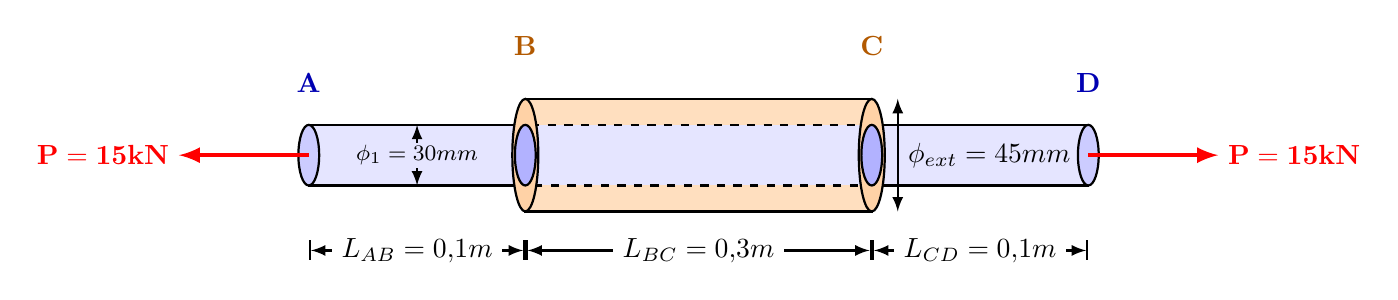
\begin{tikzpicture}[scale=1.1, >=latex]
        % Ejes y líneas de referencia
        % Tramos: A=(0,0), B=(3,0), C=(7.5,0), D=(10.5,0) (escala: 1 unidad = 0.5 dm = 0.05 m)
        % varilla d=30mm -> radio r1=0.35, camisa d=45mm -> radio r2=0.65
        
        % Tramo AB (varilla sola)
        \draw[thick, fill=blue!10] (0,-0.35) rectangle (2.5,0.35);
        
        % Tramo BC (camisa exterior)
        \draw[thick, fill=orange!25] (2.5,-0.65) rectangle (6.5,0.65);
        % Varilla interior (líneas discontinuas dentro de la camisa)
        \draw[dashed, thick, fill=blue!10] (2.5,-0.35) rectangle (6.5,0.35);
        
        % Tramo CD (varilla sola)
        \draw[thick, fill=blue!10] (6.5,-0.35) rectangle (9.0,0.35);
        
        % Tapas circulares / elipses en extremos
        \draw[thick, fill=blue!20] (0,0) ellipse (0.12 and 0.35);
        \draw[thick, fill=orange!35] (2.5,0) ellipse (0.15 and 0.65);
        \draw[thick, fill=blue!30] (2.5,0) ellipse (0.12 and 0.35);
        \draw[thick, fill=orange!35] (6.5,0) ellipse (0.15 and 0.65);
        \draw[thick, fill=blue!30] (6.5,0) ellipse (0.12 and 0.35);
        \draw[thick, fill=blue!20] (9.0,0) ellipse (0.12 and 0.35);
        
        % Cargas de tracción P = 15 kN
        \draw[ultra thick, red, <-] (-1.5,0) -- (0,0);
        \node[red, left] at (-1.5,0) {$\mathbf{P = 15\text{ kN}}$};
        \draw[ultra thick, red, ->] (9.0,0) -- (10.5,0);
        \node[red, right] at (10.5,0) {$\mathbf{P = 15\text{ kN}}$};
        
        % Letras de nudos
        \node[above=8pt, blue!70!black] at (0,0.35) {$\mathbf{A}$};
        \node[above=12pt, orange!70!black] at (2.5,0.65) {$\mathbf{B}$};
        \node[above=12pt, orange!70!black] at (6.5,0.65) {$\mathbf{C}$};
        \node[above=8pt, blue!70!black] at (9.0,0.35) {$\mathbf{D}$};
        
        % Cotas longitudinales
        \draw[|<->|, thick] (0,-1.1) -- (2.5,-1.1) node[midway, fill=white] {$L_{AB} = 0{,}1\text{ m}$};
        \draw[|<->|, thick] (2.5,-1.1) -- (6.5,-1.1) node[midway, fill=white] {$L_{BC} = 0{,}3\text{ m}$};
        \draw[|<->|, thick] (6.5,-1.1) -- (9.0,-1.1) node[midway, fill=white] {$L_{CD} = 0{,}1\text{ m}$};
        
        % Cotas diametrales (reubicadas para no solapar con la carga P = 15 kN)
        \draw[<->, thick] (1.25,-0.35) -- (1.25,0.35) node[midway, fill=blue!10, inner sep=1pt] {\footnotesize $\phi_1 = 30\text{ mm}$};
        \draw[<->, thick] (6.8,-0.65) -- (6.8,0.65) node[midway, right] {$\phi_{\text{ext}} = 45\text{ mm}$};
    \end{tikzpicture}
    \caption{Geometría de la varilla cilíndrica $AD$ con camisa concéntrica pegada en el tramo central $BC$.}
    \label{fig:varilla_camisa_geometria}
\end{figure}

\subsubsection{Cálculo de Áreas y Rigideces Axiles Elementales}

\begin{enumerate}
    \item \textbf{Sección 1 (Varilla maciza de plástico 1):}
    \begin{equation}
        A_1 = \frac{\pi}{4} d_1^2 = \frac{\pi}{4} (0{,}030\text{ m})^2 = \frac{9\pi}{4} \cdot 10^{-4}\text{ m}^2 \approx 7{,}0686 \cdot 10^{-4}\text{ m}^2 = 706{,}86\text{ mm}^2
    \end{equation}
    Rigidez axil unitaria de la varilla:
    \begin{equation}
        (E A)_1 = 3{,}1 \cdot 10^9\text{ N/m}^2 \times 7{,}0686 \cdot 10^{-4}\text{ m}^2 \approx 2{,}1913 \cdot 10^6\text{ N}
    \end{equation}

    \item \textbf{Sección 2 (Camisa tubular de plástico 2):}
    \begin{align}
        A_2 &= \frac{\pi}{4} \left(d_{\text{ext}}^2 - d_1^2\right) = \frac{\pi}{4} \left(0{,}045^2 - 0{,}030^2\right) = \frac{\pi}{4} (0{,}002025 - 0{,}000900) \nonumber \\
        &= \frac{\pi}{4} \cdot 0{,}001125\text{ m}^2 \approx 8{,}8357 \cdot 10^{-4}\text{ m}^2 = 883{,}57\text{ mm}^2
    \end{align}
    Rigidez axil unitaria de la camisa:
    \begin{equation}
        (E A)_2 = 2{,}5 \cdot 10^9\text{ N/m}^2 \times 8{,}8357 \cdot 10^{-4}\text{ m}^2 \approx 2{,}2089 \cdot 10^6\text{ N}
    \end{equation}

    \item \textbf{Rigidez equivalente combinada del tramo compuesto ($BC$):}
    Al estar perfectamente pegadas, ambas secciones experimentan el mismo alargamiento, sumándose sus rigideces:
    \begin{equation}
        (EA)_{\text{eq}} = (EA)_1 + (EA)_2 = 2{,}1913 \cdot 10^6 + 2{,}2089 \cdot 10^6 = 4{,}4002 \cdot 10^6\text{ N}
    \end{equation}
\end{enumerate}

\subsection{Apartado a) Alargamiento Total con Camisa Parcial Central}

El sistema completo está compuesto por tres tramos en serie:
\begin{equation}
    \Delta l_{\text{total}} = \Delta l_{AB} + \Delta l_{BC} + \Delta l_{CD}
\end{equation}

\subsubsection{1. Tramos extremos homogéneos AB y CD (L = 0,1 m)}

En los tramos $AB$ y $CD$, el axil de $15\text{ kN}$ lo soporta íntegramente la varilla maciza:
\begin{equation}
    N_{AB} = N_{CD} = P = 15\text{ kN} = 15\,000\text{ N}
\end{equation}
Aplicando la ley de Hooke unidimensional:
\begin{align}
    \Delta l_{AB} = \Delta l_{CD} &= \frac{P \cdot L_{AB}}{A_1 \cdot E_1} = \frac{15\,000\text{ N} \cdot 0{,}1\text{ m}}{\left(\frac{\pi}{4} \cdot 0{,}03^2\text{ m}^2\right) \cdot \left(3{,}1 \cdot 10^9\text{ N/m}^2\right)} \nonumber \\
    &= \frac{1\,500}{2\,191\,261} \approx 6{,}8454 \cdot 10^{-4}\text{ m} \approx 0{,}6845\text{ mm} \approx 0{,}68\text{ mm}
\end{align}

\subsubsection{2. Tramo central compuesto BC (L = 0,3 m)}

En el tramo $BC$, la carga externa total $P = 15\text{ kN}$ se reparte entre la varilla interna ($N_{BC,1}$) y la camisa externa ($N_{BC,2}$):
\begin{equation}
    N_{BC,1} + N_{BC,2} = P = 15\text{ kN} \label{eq:varilla_camisa_eq_estatica}
\end{equation}

Dado que no existe deslizamiento entre ambas superficies, la deformación axial relativa es nula y los alargamientos de ambos elementos en el tramo coinciden:
\begin{equation}
    \Delta l_{BC,1} = \Delta l_{BC,2} = \Delta l_{BC} \label{eq:varilla_camisa_compatibilidad}
\end{equation}
Sustituyendo por la elasticidad de cada componente:
\begin{equation}
    \frac{N_{BC,1} \cdot L_{BC}}{A_1 \cdot E_1} = \frac{N_{BC,2} \cdot L_{BC}}{A_2 \cdot E_2} \implies N_{BC,1} = N_{BC,2} \frac{A_1 E_1}{A_2 E_2}
\end{equation}
Calculando el cociente de rigideces:
\begin{equation}
    \frac{A_1 E_1}{A_2 E_2} = \frac{7{,}0686 \cdot 10^{-4} \cdot 3{,}1 \cdot 10^9}{8{,}8357 \cdot 10^{-4} \cdot 2{,}5 \cdot 10^9} = \frac{2{,}1913 \cdot 10^6}{2{,}2089 \cdot 10^6} \approx 0{,}9920
\end{equation}
Sustituyendo en la ecuación de equilibrio estático~\eqref{eq:varilla_camisa_eq_estatica}:
\begin{equation}
    0{,}9920\, N_{BC,2} + N_{BC,2} = 15\text{ kN} \implies 1{,}9920\, N_{BC,2} = 15\text{ kN}
\end{equation}
\begin{align}
    N_{BC,2} &= \frac{15}{1{,}9920} \approx \mathbf{7{,}53\text{ kN}} \quad (\text{camisa exterior}) \\
    N_{BC,1} &= 15 - 7{,}53 \approx \mathbf{7{,}47\text{ kN}} \quad (\text{varilla interior})
\end{align}
\begin{tcolorbox}[colback=blue!5!white, colframe=blue!60!black, arc=3pt, boxrule=0.7pt]
    \small \textbf{Comentario sobre la solución manuscrita:}
    En los apuntes de clase se redondeó $A_1 \approx 7{,}1 \cdot 10^{-4}\text{ m}^2$ y $A_2 \approx 8{,}83 \cdot 10^{-4}\text{ m}^2$, obteniéndose valores prácticamente simétricos: $N_{BC,1} = 7{,}49\text{ kN}$ y $N_{BC,2} = 7{,}51\text{ kN}$. Ambos cálculos confirman que la carga de $15\text{ kN}$ se reparte casi al $50\%$ entre varilla y camisa debido a la paridad de sus productos $E \cdot A$.
\end{tcolorbox}

El alargamiento del tramo $BC$ se obtiene evaluando cualquiera de las dos componentes:
\begin{align}
    \Delta l_{BC} &= \frac{N_{BC,1} \cdot L_{BC}}{A_1 \cdot E_1} = \frac{7\,470\text{ N} \cdot 0{,}3\text{ m}}{2{,}1913 \cdot 10^6\text{ N}} \approx 1{,}0229 \cdot 10^{-3}\text{ m} \approx 1{,}02\text{ mm} \approx \mathbf{1{,}00\text{ mm}}
\end{align}
O equivalentemente por la rigidez conjunta:
\begin{equation}
    \Delta l_{BC} = \frac{P \cdot L_{BC}}{(EA)_{\text{eq}}} = \frac{15\,000 \cdot 0{,}3}{4{,}4002 \cdot 10^6} = 1{,}0227 \cdot 10^{-3}\text{ m} \approx 1{,}02\text{ mm}
\end{equation}

\subsubsection{3. Alargamiento total acumulado}

Sumando las deformaciones de los tres tramos:
\begin{align}
    \Delta l_{\text{total, a}} &= \Delta l_{AB} + \Delta l_{BC} + \Delta l_{CD} = 2 \cdot \Delta l_{AB} + \Delta l_{BC} \nonumber \\
    &= 2 \cdot (0{,}6845\text{ mm}) + 1{,}0227\text{ mm} \approx 1{,}369\text{ mm} + 1{,}023\text{ mm} = \mathbf{2{,}39\text{ mm}}
\end{align}
\textit{(En las notas manuscritas redondeadas: $2 \cdot 0{,}68\text{ mm} + 1{,}00\text{ mm} = \mathbf{2{,}36\text{ mm}}$)}.

\subsection{Apartado b) Alargamiento si la Camisa se Prolonga a Toda la Varilla (L = 0,5 m)}

Si la camisa se extiende en la totalidad de la varilla ($L = 0{,}5\text{ m}$), toda la pieza trabaja como una sección compuesta solidaria de longitud completa.

\begin{figure}[H]
    \centering
    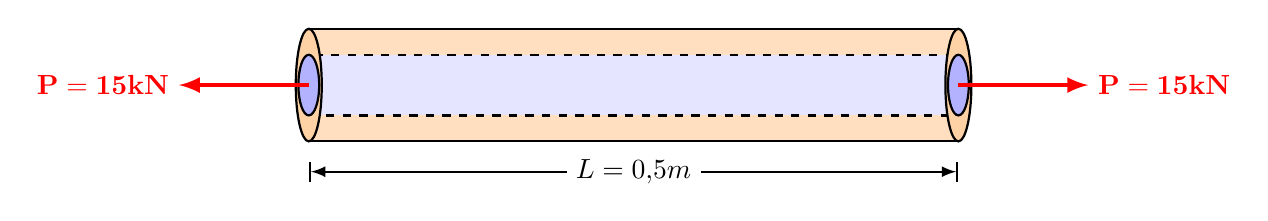
\begin{tikzpicture}[scale=1.1, >=latex]
        % Varilla totalmente encamisada
        \draw[thick, fill=orange!25] (0,-0.65) rectangle (7.5,0.65);
        \draw[dashed, thick, fill=blue!10] (0,-0.35) rectangle (7.5,0.35);
        
        \draw[thick, fill=orange!35] (0,0) ellipse (0.15 and 0.65);
        \draw[thick, fill=blue!30] (0,0) ellipse (0.12 and 0.35);
        \draw[thick, fill=orange!35] (7.5,0) ellipse (0.15 and 0.65);
        \draw[thick, fill=blue!30] (7.5,0) ellipse (0.12 and 0.35);
        
        % Cargas
        \draw[ultra thick, red, <-] (-1.5,0) -- (0,0);
        \node[red, left] at (-1.5,0) {$\mathbf{P = 15\text{ kN}}$};
        \draw[ultra thick, red, ->] (7.5,0) -- (9.0,0);
        \node[red, right] at (9.0,0) {$\mathbf{P = 15\text{ kN}}$};
        
        % Cota longitudinal
        \draw[|<->|, thick] (0,-1.0) -- (7.5,-1.0) node[midway, fill=white] {$L = 0{,}5\text{ m}$};
    \end{tikzpicture}
    \caption{Esquema de la varilla completamente encamisada a lo largo de toda su longitud ($L = 0{,}5\text{ m}$).}
    \label{fig:varilla_camisa_total}
\end{figure}

El reparto de fuerzas entre ambos materiales es idéntico al tramo $BC$ del caso anterior, al mantenerse constantes las propiedades de las secciones y módulos elásticos:
\begin{equation}
    N_1 \approx 7{,}47\text{ kN}, \qquad N_2 \approx 7{,}53\text{ kN}
\end{equation}
El alargamiento total se calcula directamente sobre la longitud total de $0{,}5\text{ m}$:
\begin{equation}
    \Delta l_{\text{total, b}} = \frac{N_1 \cdot L}{A_1 \cdot E_1} = \frac{P \cdot L}{(EA)_{\text{eq}}} = \frac{15\,000\text{ N} \cdot 0{,}5\text{ m}}{4{,}4002 \cdot 10^6\text{ N}} \approx 1{,}704 \cdot 10^{-3}\text{ m} \approx \mathbf{1{,}70\text{ mm}}
\end{equation}
*(Valor redondeado en el manuscrito: $\Delta l = 1{,}7045\text{ mm} \approx \mathbf{1{,}7\text{ mm}}$)*.

\subsection{Apartado c) Alargamiento si No Hubiera Camisa}

En ausencia total de camisa de refuerzo, la varilla maciza de plástico soporta la totalidad del esfuerzo axil $P = 15\text{ kN}$ en toda su longitud $L = 0{,}5\text{ m}$:
\begin{align}
    \Delta l_{\text{total, c}} &= \frac{P \cdot L}{A_1 \cdot E_1} = \frac{15\,000\text{ N} \cdot 0{,}5\text{ m}}{\left(\frac{\pi}{4} \cdot 0{,}03^2\text{ m}^2\right) \cdot \left(3{,}1 \cdot 10^9\text{ N/m}^2\right)} \nonumber \\
    &= \frac{7\,500}{2\,191\,261} \approx 3{,}4226 \cdot 10^{-3}\text{ m} \approx \mathbf{3{,}42\text{ mm}}
\end{align}
*(En el manuscrito se empleó $A_1 \approx 7{,}1 \cdot 10^{-4}\text{ m}^2$, resultando exactamente $\frac{7\,500}{3{,}1 \cdot 10^9 \cdot 7{,}1 \cdot 10^{-4}} \approx 0{,}0034\text{ m} = \mathbf{3{,}4\text{ mm}}$)*.

%=============================================================================
\subsection*{Resumen Comparativo de Configuraciones}

\begin{table}[H]
    \centering
    \caption{Comparación de rigidez y alargamiento de la varilla en función del encamisado ($P = 15\text{ kN}$, $L = 0{,}5\text{ m}$).}
    \vspace{2mm}
    \adjustbox{max width=0.90\textwidth}{%
        \renewcommand{\arraystretch}{1.3}
        \begin{tabular}{lcccc}
            \toprule
            \textbf{Configuración} & \textbf{Rigidez Axil Media} & \textbf{Alargamiento $\Delta l$} & \textbf{Reducción Deformación} & \textbf{Observaciones} \\
            \midrule
            \textbf{c) Sin camisa (solo varilla)} & $(EA)_1 = 2{,}19\text{ MN}$ & $\mathbf{3{,}42\text{ mm}}$ ($3{,}4\text{ mm}$) & $0\%$ (Base) & Varilla de $\phi = 30\text{ mm}$ simple \\
            \textbf{a) Camisa parcial central} & Variable por tramos & $\mathbf{2{,}39\text{ mm}}$ ($2{,}36\text{ mm}$) & $\approx 30{,}1\%$ & Camisa de $0{,}3\text{ m}$ en zona central \\
            \textbf{b) Camisa continua completa} & $(EA)_{\text{eq}} = 4{,}40\text{ MN}$ & $\mathbf{1{,}70\text{ mm}}$ ($1{,}7\text{ mm}$) & $\mathbf{50{,}3\%}$ & Duplica la rigidez axil global \\
            \bottomrule
        \end{tabular}%
    }
    \label{tab:resumen_varilla_camisa}
\end{table}

\begin{tcolorbox}[colback=myg!10!white, colframe=myg!70!black, arc=4pt, boxrule=0.9pt]
    \textbf{Conclusión Física del Problema:}
    \begin{itemize}
        \item En secciones compuestas adheridas en paralelo sometidas a axil directo, la carga total se redistribuye en proporción estricta a la rigidez elástica de cada componente:
        $$\frac{N_1}{N_2} = \frac{E_1 A_1}{E_2 A_2}$$
        \item Al extender la camisa tubular a lo largo de toda la varilla, la rigidez axil prácticamente se duplica ($4{,}40\text{ MN}$ frente a $2{,}19\text{ MN}$), logrando reducir el alargamiento a la mitad exacta ($1{,}70\text{ mm}$ frente a $3{,}42\text{ mm}$).
    \end{itemize}
\end{tcolorbox}

%=============================================================================
\section{Problema de Examen: Columna Rígida con Tirante Inclinado y Carga Lateral}

\begin{tcolorbox}[colback=white, colframe=myb!80!black, arc=4pt, boxrule=0.9pt, left=8pt, right=8pt, top=7pt, bottom=7pt]
    \textbf{Tipo de Problema:} Estructura plana articulada compuesta por una columna vertical indeformable (rígida a flexión) arriostrada mediante un tirante/cable elástico inclinado de acero. Determinación de la capacidad de carga máxima admisible frente a dos estados límite concurrentes: deformabilidad máxima horizontal (flecha o desplazamiento lateral) y resistencia máxima por rotura/tensión admisible en el cable.\\
    \textbf{Objetivos a Determinar:}
    \begin{enumerate}
        \item Carga lateral máxima $P_{\delta}$ admisible para no superar el desplazamiento horizontal admisible del extremo superior $B$: $\delta_{B,h} \leq 11\text{ cm} = 0{,}11\text{ m}$.
        \item Esfuerzo axil máximo $N_{BC,\text{máx}}$ y carga admisible $P_{\sigma}$ para no superar la tensión admisible del cable de acero: $\sigma_{\text{adm}} = 190\text{ N/mm}^2 = 190\text{ MPa}$.
        \item Carga máxima admisible de servicio global del sistema: $P_{\text{máx}} = \min(P_{\delta}, P_{\sigma})$.
    \end{enumerate}
\end{tcolorbox}

\subsection{Enunciado y Geometría de Partida}

Se considera la estructura mostrada en la figura, formada por una columna vertical $AB$ considerada infinitamente rígida e indeformable, articulada en su base $A$ mediante un apoyo fijo. La altura total de la columna es:
\begin{equation}
    H = L_{AB} = 3{,}5\text{ m} + 2{,}5\text{ m} = 6{,}0\text{ m}
\end{equation}
Sobre la columna actúa una carga horizontal puntual $P$ hacia la izquierda, aplicada a una cota de $3{,}5\text{ m}$ sobre la base ($2{,}5\text{ m}$ por debajo del extremo superior $B$).

Para impedir el vuelco y restringir el desplazamiento lateral de la columna, se ancla en su cúspide $B$ un cable elástico de acero $BC$, que se fija a tierra en un punto rígido $C$ situado al nivel del suelo a una distancia horizontal de $4{,}0\text{ m}$ respecto al eje de la columna. El anclaje $C$ es un punto de apoyo fijo independiente.

\begin{figure}[H]
    \centering
    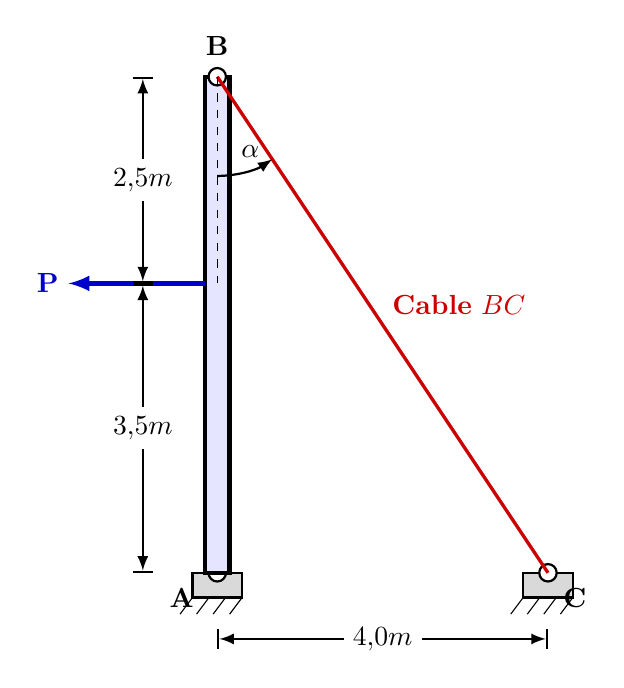
\begin{tikzpicture}[scale=1.05, >=latex]
        % Apoyo A en (0,0)
        \draw[thick, fill=gray!30] (-0.3,-0.3) rectangle (0.3,0);
        \draw (-0.3,-0.3) -- (-0.45,-0.5);
        \draw (-0.1,-0.3) -- (-0.25,-0.5);
        \draw (0.1,-0.3) -- (-0.05,-0.5);
        \draw (0.3,-0.3) -- (0.15,-0.5);
        \draw[thick, fill=white] (0,0) circle (3pt);
        \node[below left=2pt] at (-0.1,0) {$\mathbf{A}$};
        
        % Barra vertical rígida AB
        \draw[ultra thick, fill=blue!10] (-0.15,0) rectangle (0.15,6.0);
        \draw[thick, fill=white] (0,6.0) circle (3pt);
        \node[above=4pt] at (0,6.0) {$\mathbf{B}$};
        
        % Anclaje C en (4.0, 0)
        \draw[thick, fill=gray!30] (3.7,-0.3) rectangle (4.3,0);
        \draw (3.7,-0.3) -- (3.55,-0.5);
        \draw (3.9,-0.3) -- (3.75,-0.5);
        \draw (4.1,-0.3) -- (3.95,-0.5);
        \draw (4.3,-0.3) -- (4.15,-0.5);
        \draw[thick, fill=white] (4.0,0) circle (3pt);
        \node[below right=2pt] at (4.0,0) {$\mathbf{C}$};
        
        % Cable BC
        \draw[very thick, red!80!black] (0,6.0) -- (4.0,0);
        \node[red!80!black, above right] at (2.0,3.0) {\textbf{Cable} $BC$};
        
        % Carga horizontal P en y = 3.5m
        \draw[ultra thick, blue!80!black, <-] (-1.8,3.5) -- (-0.15,3.5);
        \node[blue!80!black, left] at (-1.8,3.5) {$\mathbf{P}$};
        
        % Ángulo alfa en B
        \draw[dashed, thin] (0,6.0) -- (0,3.5);
        \draw[thick, ->] (0,4.8) arc (-90:-56.3:1.2);
        \node at (0.4,5.1) {$\alpha$};
        
        % Cotas verticales
        \draw[|<->|, thick] (-0.9,0) -- (-0.9,3.5) node[midway, fill=white] {$3{,}5\text{ m}$};
        \draw[|<->|, thick] (-0.9,3.5) -- (-0.9,6.0) node[midway, fill=white] {$2{,}5\text{ m}$};
        
        % Cota horizontal
        \draw[|<->|, thick] (0,-0.8) -- (4.0,-0.8) node[midway, fill=white] {$4{,}0\text{ m}$};
    \end{tikzpicture}
    \caption{Geometría de la columna rígida $AB$ arriostrada mediante el cable inclinado $BC$.}
    \label{fig:columna_tirante_geometria}
\end{figure}

\subsubsection{Propiedades Mecánicas y Geométricas del Cable}

\begin{itemize}
    \item \textbf{Diámetro nominal del cable:} $\phi = 4\text{ mm} = 4 \cdot 10^{-3}\text{ m}$.
    \item \textbf{Sección transversal del cable ($\Omega$):}
    \begin{equation}
        \Omega = \frac{\pi}{4}\phi^2 = \frac{\pi}{4}(4 \cdot 10^{-3}\text{ m})^2 = 4\pi \cdot 10^{-6}\text{ m}^2 \approx 1{,}2566 \cdot 10^{-5}\text{ m}^2 = 12{,}566\text{ mm}^2
    \end{equation}
    \item \textbf{Módulo de elasticidad longitudinal ($E$):}
    \begin{equation}
        E = 20\,000\text{ kN/cm}^2 = 20\,000 \cdot \frac{10^3\text{ N}}{10^{-4}\text{ m}^2} = 2 \cdot 10^{11}\text{ N/m}^2 = 200\text{ GPa}
    \end{equation}
    \item \textbf{Tensión admisible de rotura/servicio ($\sigma_{\text{adm}}$):}
    \begin{equation}
        \sigma_{\text{adm}} = 190\text{ N/mm}^2 = 190\text{ MPa} = 190 \cdot 10^6\text{ N/m}^2
    \end{equation}
    \item \textbf{Desplazamiento horizontal máximo admisible de la cúspide $B$:}
    \begin{equation}
        \delta_{B,h} = \overline{BB''} \leq 11\text{ cm} = 0{,}11\text{ m}
    \end{equation}
    \item \textbf{Longitud y orientación geométrica del cable $BC$:}
    \begin{align}
        L_C &= \sqrt{4{,}0^2 + 6{,}0^2} = \sqrt{16 + 36} = \sqrt{52}\text{ m} \approx 7{,}2111\text{ m} \approx 7{,}21\text{ m} \\
        \tan \alpha &= \frac{4{,}0}{6{,}0} = \frac{2}{3} \implies \alpha = \arctan\left(\frac{2}{3}\right) \approx 33{,}69^\circ \\
        \sin \alpha &= \frac{4}{\sqrt{52}} = \frac{2}{\sqrt{13}} \approx 0{,}5547 \\
        \cos \alpha &= \frac{6}{\sqrt{52}} = \frac{3}{\sqrt{13}} \approx 0{,}8321
    \end{align}
\end{itemize}

\subsection{Equilibrio Estático de la Columna Rígida}

Aislando la columna rígida $AB$, las fuerzas que intervienen en su Diagrama de Sólido Libre (DCL) son:
\begin{enumerate}
    \item Reacciones en el apoyo fijo $A$: componente horizontal $H_A$ ($\rightarrow$) y componente vertical $V_A$ ($\uparrow$).
    \item Carga horizontal exterior aplicada $P$ ($\leftarrow$) a cota $y = 3{,}5\text{ m}$.
    \item Acción del cable $BC$ sobre la cúspide $B$: fuerza de tracción $N_{BC}$ dirigida a lo largo del cable hacia el anclaje $C$, cuyas componentes son:
    \begin{align}
        N_{BC,x} &= N_{BC} \sin\alpha \quad (\rightarrow) \\
        N_{BC,y} &= N_{BC} \cos\alpha \quad (\downarrow)
    \end{align}
\end{enumerate}

\begin{figure}[H]
    \centering
    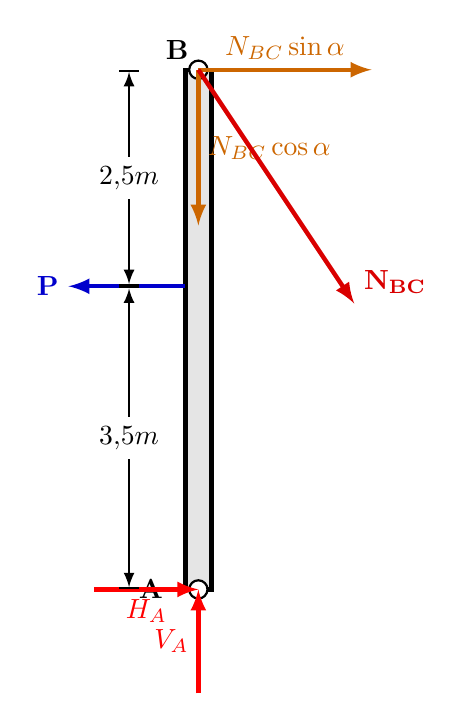
\begin{tikzpicture}[scale=1.1, >=latex]
        % Columna
        \draw[ultra thick, fill=gray!20] (-0.15,0) rectangle (0.15,6.0);
        
        % Apoyo A
        \draw[thick, fill=white] (0,0) circle (3pt);
        \node[left=3pt] at (-0.2,0) {$\mathbf{A}$};
        \draw[ultra thick, red, ->] (-1.2,0) -- (0,0);
        \node[red, below] at (-0.6,0) {$H_A$};
        \draw[ultra thick, red, ->] (0,-1.2) -- (0,0);
        \node[red, left] at (0,-0.6) {$V_A$};
        
        % Carga P
        \draw[ultra thick, blue!80!black, <-] (-1.5,3.5) -- (-0.15,3.5);
        \node[blue!80!black, left] at (-1.5,3.5) {$\mathbf{P}$};
        
        % Descomposición de la fuerza en B
        \draw[thick, fill=white] (0,6.0) circle (3pt);
        \node[above left] at (0,6.0) {$\mathbf{B}$};
        \draw[ultra thick, orange!80!black, ->] (0,6.0) -- (2.0,6.0);
        \node[orange!80!black, above] at (1.0,6.0) {$N_{BC} \sin\alpha$};
        \draw[ultra thick, orange!80!black, ->] (0,6.0) -- (0,4.2);
        \node[orange!80!black, right] at (0,5.1) {$N_{BC} \cos\alpha$};
        \draw[ultra thick, red!85!black, ->] (0,6.0) -- (1.8,3.3);
        \node[red!85!black, above right] at (1.8,3.3) {$\mathbf{N_{BC}}$};
        
        % Cotas
        \draw[|<->|, thick] (-0.8,0) -- (-0.8,3.5) node[midway, fill=white] {$3{,}5\text{ m}$};
        \draw[|<->|, thick] (-0.8,3.5) -- (-0.8,6.0) node[midway, fill=white] {$2{,}5\text{ m}$};
    \end{tikzpicture}
    \caption{Diagrama de Sólido Libre (DCL) de la columna rígida $AB$.}
    \label{fig:columna_dcl}
\end{figure}

Planteando las tres ecuaciones de equilibrio estático en el plano:
\begin{align}
    \sum F_x = 0 &\implies H_A - P + N_{BC} \sin\alpha = 0 \label{eq:columna_fx} \\
    \sum F_y = 0 &\implies V_A - N_{BC} \cos\alpha = 0 \label{eq:columna_fy} \\
    \sum M_A = 0 &\implies P \cdot 3{,}5 - (N_{BC} \sin\alpha) \cdot 6{,}0 = 0 \label{eq:columna_ma}
\end{align}

De la ecuación de momentos~\eqref{eq:columna_ma} se obtiene la relación directa e independiente entre la fuerza del tirante $N_{BC}$ y la carga lateral $P$:
\begin{equation}
    P \cdot 3{,}5 = N_{BC} \cdot 6{,}0 \cdot \sin(33{,}69^\circ) = N_{BC} \cdot 6{,}0 \cdot \frac{2}{\sqrt{13}} \approx 3{,}3282 \, N_{BC}
\end{equation}
\begin{equation}
    P = \frac{6{,}0 \cdot \sin(33{,}69^\circ)}{3{,}5} N_{BC} \approx 0{,}9509 \, N_{BC} \label{eq:relacion_p_nbc}
\end{equation}

\subsection{Análisis Cinemático y Condición de Compatibilidad}

Al ser la barra $AB$ rígida e indeformable articulada en $A$, su deformada corresponde a una rotación pura de sólido rígido alrededor de $A$ por un ángulo infinitesimal $\theta$.
El extremo $B$ sufre un desplazamiento horizontal:
\begin{equation}
    \delta_{B,h} = \overline{BB''} = H \cdot \theta \leq 0{,}11\text{ m}
\end{equation}

\begin{figure}[H]
    \centering
    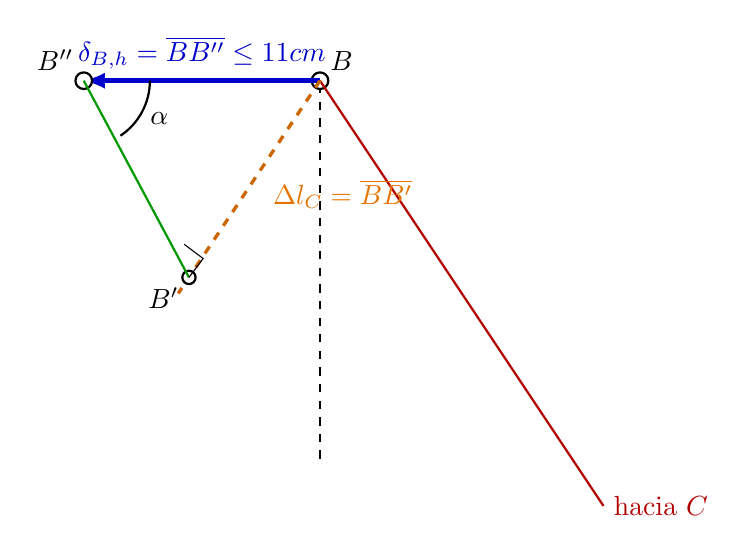
\begin{tikzpicture}[scale=1.2, >=latex]
        % Triángulo cinemático en el nudo B
        \coordinate (B) at (0,4);
        \coordinate (Bpp) at (-2.5,4); % Desplazamiento horizontal B''
        \coordinate (Bp) at (-1.387,1.919); % Proyección sobre la dirección del cable
        
        % Línea original de la barra
        \draw[thick, dashed] (0,0) -- (B);
        \draw[thick, fill=white] (B) circle (2.5pt) node[above right] {$B$};
        
        % Cable original hacia C
        \draw[thick, red!70!black] (B) -- (3, -0.5) node[right] {hacia $C$};
        
        % Desplazamiento horizontal BB''
        \draw[ultra thick, blue!80!black, ->] (B) -- (Bpp) node[midway, above] {$\delta_{B,h} = \overline{BB''} \leq 11\text{ cm}$};
        \draw[thick, fill=white] (Bpp) circle (2.5pt) node[above left] {$B''$};
        
        % Alargamiento del cable Delta l_C = BB'
        \draw[very thick, dashed, orange!80!black] (B) -- (-1.5,1.75);
        \draw[thick, fill=white] (-1.387,1.919) circle (2pt) node[below left] {$B'$};
        
        % Triángulo rectángulo B - B' - B''
        \draw[thick, green!60!black] (Bpp) -- (-1.387,1.919);
        
        % Ángulo recto en B'
        \draw[thin] (-1.387,1.919) -- ++(0.15,0.2) -- ++(-0.2,0.15);
        
        % Cota de alargamiento Delta l
        \node[orange!90!black, right] at (-0.6,2.8) {$\Delta l_C = \overline{BB'}$};
        
        % Ángulo alfa
        \draw[thick] (Bpp) ++(0.7,0) arc (0:-56.3:0.7);
        \node at (-1.7,3.6) {$\alpha$};
    \end{tikzpicture}
    \caption{Cinemática del nudo $B$: proyección geométrica del desplazamiento lateral $\delta_{B,h}$ en el alargamiento axial del cable $\Delta l_C$.}
    \label{fig:cinematica_cable}
\end{figure}

Proyectando el desplazamiento horizontal $\delta_{B,h} = \overline{BB''}$ sobre la directriz del cable inclinado (formando el triángulo rectángulo $BB'B''$ con ángulo recto en $B'$):
\begin{equation}
    \sin\alpha = \frac{\Delta l_C}{\overline{BB''}} \implies \Delta l_C = \overline{BB''} \cdot \sin\alpha \label{eq:compatibilidad_cable}
\end{equation}

Sustituyendo el desplazamiento horizontal admisible $\overline{BB''} \leq 0{,}11\text{ m}$:
\begin{equation}
    \Delta l_{C,\text{máx}} = 0{,}11\text{ m} \cdot \sin(33{,}69^\circ) = 0{,}11 \cdot 0{,}5547 \approx 0{,}0610\text{ m} = 61{,}0\text{ mm}
\end{equation}

\subsection{Cálculo de la Capacidad de Carga Frente a Cada Estado Límite}

\subsubsection{1. Limitación por Deformabilidad (Flecha máxima admisible)}

Relacionando el alargamiento elástico del cable con su ley constitutiva (Hooke):
\begin{equation}
    \Delta l_C = \frac{N_{BC} \cdot L_C}{\Omega \cdot E} \implies N_{BC,\delta} = \frac{\Delta l_{C,\text{máx}} \cdot \Omega \cdot E}{L_C}
\end{equation}
Sustituyendo los valores numéricos del sistema:
\begin{align}
    N_{BC,\delta} &= \frac{0{,}0610\text{ m} \cdot \left(1{,}2566 \cdot 10^{-5}\text{ m}^2\right) \cdot \left(2 \cdot 10^{11}\text{ N/m}^2\right)}{7{,}2111\text{ m}} \nonumber \\
    &= \frac{153\,305{,}2}{7{,}2111} \approx 21\,259{,}6\text{ N} \approx \mathbf{21{,}26\text{ kN}}
\end{align}
A partir del equilibrio de momentos~\eqref{eq:columna_ma}, la carga exterior $P$ asociada a este límite de deformación es:
\begin{equation}
    P_{\delta} = \frac{6{,}0 \cdot \sin(33{,}69^\circ)}{3{,}5} \cdot 21{,}26\text{ kN} \approx \mathbf{20{,}21\text{ kN}}
\end{equation}

\subsubsection{2. Comprobación y Limitación por Tensión Admisible}

Si se aplicara la carga calculada por deformación ($N_{BC} = 21{,}26\text{ kN}$), la tensión de trabajo efectiva en el cable resultaría:
\begin{equation}
    \sigma = \frac{N_{BC,\delta}}{\Omega} = \frac{21\,260\text{ N}}{12{,}566\text{ mm}^2} \approx 1\,691{,}9\text{ N/mm}^2 \approx \mathbf{1692\text{ MPa}} \gg \sigma_{\text{adm}} = 190\text{ MPa}
\end{equation}
\begin{tcolorbox}[colback=red!10!white, colframe=red!80!black, arc=3pt, boxrule=0.9pt]
    \textbf{¡Aviso de Inadmisibilidad!:}\\
    La tensión de $1692\text{ MPa}$ supera en casi 9 veces la tensión admisible del acero ($\sigma_{\text{adm}} = 190\text{ MPa}$). Por tanto, \textbf{el cable rompería plásticamente mucho antes} de alcanzar el desplazamiento horizontal de $11\text{ cm}$. La resistencia del cable es el estado límite crítico determinante.
\end{tcolorbox}

Por consiguiente, el esfuerzo axil máximo admisible que el cable de $4\text{ mm}$ puede soportar con seguridad es:
\begin{align}
    N_{BC,\text{adm}} &= \sigma_{\text{adm}} \cdot \Omega = 190\text{ N/mm}^2 \times 12{,}566\text{ mm}^2 \nonumber \\
    &= 2\,387{,}54\text{ N} \approx \mathbf{2{,}39\text{ kN}}
\end{align}

Sustituyendo este esfuerzo axil en la ecuación de momentos~\eqref{eq:columna_ma}:
\begin{equation}
    P_{\sigma} = \frac{6{,}0 \cdot \sin(33{,}69^\circ)}{3{,}5} \cdot 2{,}3875\text{ kN} = 0{,}9509 \cdot 2{,}3875\text{ kN} \approx \mathbf{2{,}27\text{ kN}}
\end{equation}

\subsubsection{3. Desplazamiento Real en Régimen Admisible}

Bajo la carga admisible real de $P = 2{,}27\text{ kN}$, el alargamiento y el desplazamiento horizontal en $B$ resultan:
\begin{align}
    \Delta l_C &= \frac{N_{BC,\text{adm}} \cdot L_C}{\Omega \cdot E} = \frac{\sigma_{\text{adm}} \cdot L_C}{E} = \frac{190 \cdot 10^6\text{ N/m}^2 \cdot 7{,}2111\text{ m}}{2 \cdot 10^{11}\text{ N/m}^2} \approx 6{,}85\text{ mm} \\
    \delta_{B,h} &= \frac{\Delta l_C}{\sin\alpha} = \frac{6{,}85\text{ mm}}{\sin(33{,}69^\circ)} \approx \mathbf{12{,}35\text{ mm}} = 1{,}24\text{ cm} \ll 11\text{ cm}
\end{align}

\subsection{Cálculo de Reacciones en la Base A}

Bajo la carga de servicio máxima admisible $P_{\text{máx}} = 2{,}27\text{ kN}$ ($N_{BC} = 2{,}39\text{ kN}$):
\begin{align}
    H_A &= P - N_{BC}\sin\alpha = 2{,}27\text{ kN} - 2{,}39 \cdot 0{,}5547\text{ kN} \approx 2{,}27 - 1{,}33 = \mathbf{0{,}94\text{ kN}} \quad (\rightarrow) \\
    V_A &= N_{BC}\cos\alpha = 2{,}39 \cdot 0{,}8321\text{ kN} \approx \mathbf{1{,}99\text{ kN}} \quad (\uparrow)
\end{align}

%=============================================================================
\subsection*{Resumen Final de Resultados}

\begin{table}[H]
    \centering
    \caption{Comparación de estados límites y dimensionamiento de la carga admisible $P$.}
    \vspace{2mm}
    \adjustbox{max width=0.98\textwidth}{%
        \renewcommand{\arraystretch}{1.25}
        \begin{tabular}{lccc}
            \toprule
            \textbf{Criterio / Condición} & \textbf{Esfuerzo Cable $N_{BC}$} & \textbf{Carga Lateral $P$} & \textbf{Estado / Diagnóstico} \\
            \midrule
            \textbf{1. Deformabilidad ($\delta_B \leq 11\text{ cm}$)} & $21{,}26\text{ kN}$ & $20{,}21\text{ kN}$ & Inadmisible ($\sigma = 1692\text{ MPa} \gg \sigma_{\text{adm}}$) \\
            \textbf{2. Tensión Admisible ($\sigma \leq 190\text{ MPa}$)} & $\mathbf{2{,}39\text{ kN}}$ & $\mathbf{2{,}27\text{ kN}}$ & \textbf{Límite Determinante (Válido)} \\
            \midrule
            \multicolumn{4}{l}{\textbf{Respuesta Final:} $\mathbf{P_{\text{máx}} = 2{,}27\text{ kN}}$ (Desplazamiento horizontal resultante: $\delta_B = 1{,}24\text{ cm} \leq 11\text{ cm}$)} \\
            \bottomrule
        \end{tabular}%
    }
    \label{tab:resumen_columna_tirante}
\end{table}

\begin{tcolorbox}[colback=myg!10!white, colframe=myg!70!black, arc=4pt, boxrule=0.9pt]
    \textbf{Nota Conceptual del Problema:}
    \begin{itemize}
        \item Cuando en un problema de resistencia de materiales se imponen simultáneamente condiciones de \textbf{deformabilidad máxima} (rigidez/flecha) y de \textbf{tensión admisible} (resistencia), la capacidad de carga real de la estructura viene estrictamente fijada por el mínimo de ambas:
        $$P_{\text{máx}} = \min(P_{\delta}, P_{\sigma})$$
        \item En este caso, el cable de $\phi = 4\text{ mm}$ es muy esbelto, por lo que alcanza su límite resistente con una deformación elástica moderada ($1{,}24\text{ cm}$), quedando la restricción geométrica de $11\text{ cm}$ con un amplio margen de seguridad.
    \end{itemize}
\end{tcolorbox}

%=============================================================================
\section{Problema de Examen: Barra Escalonada Biapoyada Bajo Peso Propio (Febrero 2016)}

\begin{tcolorbox}[colback=white, colframe=myb!80!black, arc=4pt, boxrule=0.9pt, left=8pt, right=8pt, top=7pt, bottom=7pt]
    \textbf{Tipo de Problema:} Barra vertical escalonada de dos tramos de diferente sección transversal, coaccionada axialmente en ambos extremos (biapoyada / biempotrada axil) y solicitada exclusivamente por su \textbf{peso propio continuo}.\\
    \textbf{Objetivos a Determinar:}
    \begin{enumerate}[label=\alph*)]
        \item Reacciones en los apoyos extremos ($R_A$ y $R_C$).
        \item Ley analítica y diagramas de esfuerzos axiles $N(x)$ y tensiones normales $\sigma(x)$ a lo largo de toda la barra $ABC$.
    \end{enumerate}
\end{tcolorbox}

\subsection{Enunciado y Geometría de Partida}

Se considera una barra vertical de directriz recta escalonada en dos tramos, anclada en sus extremos superior $A$ e inferior $C$ mediante apoyos rígidos que impiden todo desplazamiento vertical ($\Delta L_{AC} = 0$).

\begin{figure}[H]
    \centering
    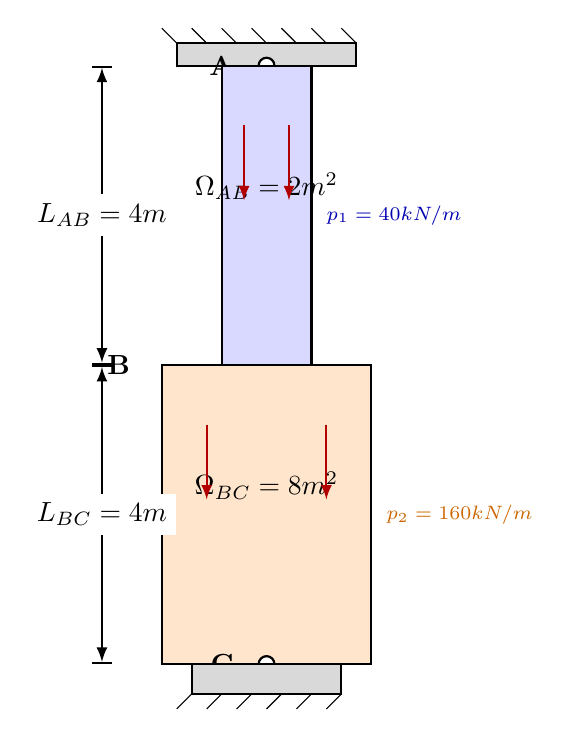
\begin{tikzpicture}[scale=0.95, >=latex]
        % Apoyo superior A
        \draw[thick, fill=gray!30] (-1.2,8) rectangle (1.2,8.3);
        \draw (-1.2,8.3) -- (-1.4,8.5);
        \draw (-0.8,8.3) -- (-1.0,8.5);
        \draw (-0.4,8.3) -- (-0.6,8.5);
        \draw (0.0,8.3) -- (-0.2,8.5);
        \draw (0.4,8.3) -- (0.2,8.5);
        \draw (0.8,8.3) -- (0.6,8.5);
        \draw (1.2,8.3) -- (1.0,8.5);
        \draw[thick, fill=white] (0,8) circle (3pt);
        \node[left=3pt] at (-0.2,8) {$\mathbf{A}$};
        
        % Tramo superior AB (Sección menor Omega_1 = 2 m^2)
        \draw[thick, fill=blue!15] (-0.6,4) rectangle (0.6,8);
        \node[above=2pt] at (0,6) {$\Omega_{AB} = 2\text{ m}^2$};
        \node[right=2pt, font=\scriptsize, blue!70!black] at (0.6,6) {$p_1 = 40\text{ kN/m}$};
        
        % Flechas de peso propio en AB
        \draw[thick, red!70!black, ->] (-0.3,7.2) -- (-0.3,6.2);
        \draw[thick, red!70!black, ->] (0.3,7.2) -- (0.3,6.2);
        
        % Nudo intermedio B
        \node[left=8pt] at (-1.4,4) {$\mathbf{B}$};
        
        % Tramo inferior BC (Sección mayor Omega_2 = 8 m^2)
        \draw[thick, fill=orange!20] (-1.4,0) rectangle (1.4,4);
        \node[above=2pt] at (0,2) {$\Omega_{BC} = 8\text{ m}^2$};
        \node[right=2pt, font=\scriptsize, orange!80!black] at (1.4,2) {$p_2 = 160\text{ kN/m}$};
        
        % Flechas de peso propio en BC
        \draw[thick, red!70!black, ->] (-0.8,3.2) -- (-0.8,2.2);
        \draw[thick, red!70!black, ->] (0.8,3.2) -- (0.8,2.2);
        
        % Apoyo inferior C
        \draw[thick, fill=white] (0,0) circle (3pt);
        \node[left=3pt] at (-0.2,0) {$\mathbf{C}$};
        \draw[thick, fill=gray!30] (-1.0,-0.4) rectangle (1.0,0);
        \draw (-1.0,-0.4) -- (-1.2,-0.6);
        \draw (-0.6,-0.4) -- (-0.8,-0.6);
        \draw (-0.2,-0.4) -- (-0.4,-0.6);
        \draw (0.2,-0.4) -- (0.0,-0.6);
        \draw (0.6,-0.4) -- (0.4,-0.6);
        \draw (1.0,-0.4) -- (0.8,-0.6);
        
        % Cotas verticales
        \draw[|<->|, thick] (-2.2,4) -- (-2.2,8) node[midway, fill=white] {$L_{AB} = 4\text{ m}$};
        \draw[|<->|, thick] (-2.2,0) -- (-2.2,4) node[midway, fill=white] {$L_{BC} = 4\text{ m}$};
    \end{tikzpicture}
    \caption{Geometría de la columna vertical escalonada biapoyada solicitada por su propio peso.}
    \label{fig:barra_escalonada_geometria}
\end{figure}

Las propiedades geométricas y mecánicas del conjunto son:
\begin{itemize}
    \item \textbf{Peso específico del material:} $\gamma = 20\text{ kN/m}^3$.
    \item \textbf{Módulo de elasticidad longitudinal:} $E = \text{constante}$.
    \item \textbf{Tramo superior $AB$:} Longitud $L_1 = 4\text{ m}$, sección transversal $\Omega_1 = \Omega_{AB} = 2\text{ m}^2$.
    Carga lineal uniforme debida al peso propio:
    \begin{equation}
        p_1 = \gamma \cdot \Omega_1 = 20\text{ kN/m}^3 \times 2\text{ m}^2 = 40\text{ kN/m} \quad (\downarrow)
    \end{equation}
    Peso total del tramo $AB$:
    \begin{equation}
        P_{AB} = p_1 \cdot L_1 = 40\text{ kN/m} \times 4\text{ m} = 160\text{ kN}
    \end{equation}
    \item \textbf{Tramo inferior $BC$:} Longitud $L_2 = 4\text{ m}$, sección transversal $\Omega_2 = \Omega_{BC} = 8\text{ m}^2$.
    Carga lineal uniforme debida al peso propio:
    \begin{equation}
        p_2 = \gamma \cdot \Omega_2 = 20\text{ kN/m}^3 \times 8\text{ m}^2 = 160\text{ kN/m} \quad (\downarrow)
    \end{equation}
    Peso total del tramo $BC$:
    \begin{equation}
        P_{BC} = p_2 \cdot L_2 = 160\text{ kN/m} \times 4\text{ m} = 640\text{ kN}
    \end{equation}
    \item \textbf{Peso total de la barra:}
    \begin{equation}
        P_{\text{total}} = P_{AB} + P_{BC} = 160\text{ kN} + 640\text{ kN} = 800\text{ kN}
    \end{equation}
\end{itemize}

\subsection{Equilibrio Estático Global}

Para facilitar la formulación analítica de las secciones, orientamos la barra en posición horizontal con el origen de coordenadas $x = 0$ situado en el extremo inferior $C$ y avanzando hacia $A$ ($x \in [0, 8\text{ m}]$):
\begin{itemize}
    \item $x = 0$: Apoyo $C$ (reacción axial $H_C$ hacia la derecha).
    \item $x \in [0, 4\text{ m}]$: Tramo $BC$ (carga lineal $p_2 = 160\text{ kN/m}$ dirigida hacia $C$, $\leftarrow$).
    \item $x = 4\text{ m}$: Nudo de cambio de sección $B$.
    \item $x \in [4, 8\text{ m}]$: Tramo $AB$ (carga lineal $p_1 = 40\text{ kN/m}$ dirigida hacia $C$, $\leftarrow$).
    \item $x = 8\text{ m}$: Apoyo $A$ (reacción axial $H_A$ hacia la derecha).
\end{itemize}

\begin{figure}[H]
    \centering
    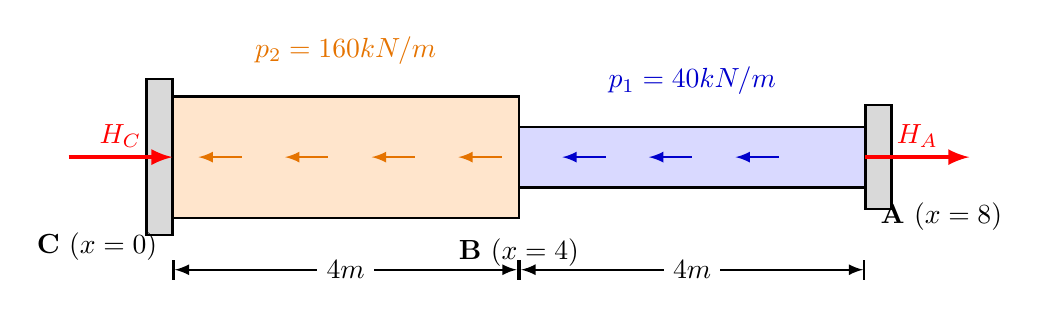
\begin{tikzpicture}[scale=1.1, >=latex]
        % Barra horizontal C -> B -> A
        \draw[thick, fill=orange!20] (0,-0.7) rectangle (4,0.7);
        \draw[thick, fill=blue!15] (4,-0.35) rectangle (8,0.35);
        
        % Apoyos
        \draw[thick, fill=gray!30] (-0.3,-0.9) rectangle (0,0.9);
        \draw[thick, fill=gray!30] (8,-0.6) rectangle (8.3,0.6);
        
        % Reacciones
        \draw[ultra thick, red, ->] (-1.2,0) -- (0,0);
        \node[red, above] at (-0.6,0) {$H_C$};
        \draw[ultra thick, red, ->] (8,0) -- (9.2,0);
        \node[red, above] at (8.6,0) {$H_A$};
        
        % Flechas de carga distribuida (peso hacia C, es decir, hacia la izquierda)
        \foreach \i in {0.8, 1.8, 2.8, 3.8} {
            \draw[thick, orange!90!black, <-] (\i-0.5,0) -- (\i,0);
        }
        \node[orange!90!black, above=8pt] at (2,0.7) {$p_2 = 160\text{ kN/m}$};
        
        \foreach \i in {5.0, 6.0, 7.0} {
            \draw[thick, blue!80!black, <-] (\i-0.5,0) -- (\i,0);
        }
        \node[blue!80!black, above=8pt] at (6,0.35) {$p_1 = 40\text{ kN/m}$};
        
        % Cotas y nudos
        \node[below left=2pt] at (0,-0.7) {$\mathbf{C}$ ($x = 0$)};
        \node[below=4pt] at (4,-0.7) {$\mathbf{B}$ ($x = 4$)};
        \node[below right=2pt] at (8,-0.35) {$\mathbf{A}$ ($x = 8$)};
        
        \draw[|<->|, thick] (0,-1.3) -- (4,-1.3) node[midway, fill=white] {$4\text{ m}$};
        \draw[|<->|, thick] (4,-1.3) -- (8,-1.3) node[midway, fill=white] {$4\text{ m}$};
    \end{tikzpicture}
    \caption{Modelo equivalente horizontal con origen de coordenadas en el apoyo inferior $C$.}
    \label{fig:barra_horizontal_dcl}
\end{figure}

Planteando el equilibrio de fuerzas axiles horizontales:
\begin{equation}
    \sum F_x = 0 \implies H_A + H_C - P_{\text{total}} = 0 \implies H_A + H_C = 800\text{ kN} \label{eq:escalonada_equilibrio}
\end{equation}
El problema presenta 1 grado de hiperestatismo (2 incógnitas de reacción para 1 ecuación de equilibrio axial no trivial).

\subsection{Ecuación de Compatibilidad de Deformaciones}

Los apoyos rígidos en $A$ y $C$ impiden el desplazamiento relativo total entre ambos extremos:
\begin{equation}
    \Delta L_{AC} = \Delta L_{BC} + \Delta L_{AB} = 0 \label{eq:escalonada_compatibilidad}
\end{equation}
Expresando el alargamiento elástico en función de la ley del esfuerzo axil $N(x)$:
\begin{equation}
    \Delta L_{AC} = \int_{0}^{4} \frac{N(x)}{\Omega_2 E}\,dx + \int_{4}^{8} \frac{N(x)}{\Omega_1 E}\,dx = 0
\end{equation}
Al ser el módulo elástico $E$ constante en toda la barra, se simplifica directamente:
\begin{equation}
    \frac{1}{\Omega_2} \int_{0}^{4} N(x)\,dx + \frac{1}{\Omega_1} \int_{4}^{8} N(x)\,dx = 0 \implies \frac{1}{8} \int_{0}^{4} N(x)\,dx + \frac{1}{2} \int_{4}^{8} N(x)\,dx = 0 \label{eq:escalonada_integral}
\end{equation}

\begin{tcolorbox}[colback=blue!5!white, colframe=blue!60!black, arc=3pt, boxrule=0.7pt]
    \small \textbf{Consejo Metodológico Clave (Anotación del Examen):}
    Si planteamos los cortes por secciones siempre mirando hacia la izquierda (desde el apoyo $C$, $x = 0$), en la ley de axiles $N(x)$ de ambos tramos solo intervendrá la reacción $H_C$. De esta forma, la ecuación de compatibilidad se resuelve con una única incógnita directa, evitando resolver sistemas de ecuaciones simultáneos acoplados.
\end{tcolorbox}

\subsubsection{Leyes del Esfuerzo Axil por Tramos}

\begin{enumerate}
    \item \textbf{Tramo 1: $BC$ ($x \in [0, 4\text{ m}]$, sección $\Omega_2 = 8\text{ m}^2$)}:
    Cortando a una distancia $x$ desde $C$ y aislando la parte izquierda:
    \begin{equation}
        \sum F_x = 0 \implies H_C - p_2 \cdot x + N(x) = 0
    \end{equation}
    \begin{equation}
        N(x) = 160\,x - H_C \label{eq:axil_tramo1}
    \end{equation}

    \item \textbf{Tramo 2: $AB$ ($x \in [4, 8\text{ m}]$, sección $\Omega_1 = 2\text{ m}^2$)}:
    Cortando en el tramo $AB$ a una distancia $x$ desde $C$ (abarcando todo el tramo $BC$ de $4\text{ m}$ y una longitud $x - 4$ del tramo $AB$):
    \begin{equation}
        \sum F_x = 0 \implies H_C - 160(4) - 40(x - 4) + N(x) = 0
    \end{equation}
    \begin{equation}
        N(x) = H_C - 640 - 40x + 160 + N(x) = 0 \implies N(x) = 40\,x - H_C + 480 \label{eq:axil_tramo2}
    \end{equation}
\end{enumerate}

\subsection{Resolución de las Reacciones en los Apoyos}

Sustituyendo las leyes de esfuerzos~\eqref{eq:axil_tramo1} y \eqref{eq:axil_tramo2} en la ecuación de compatibilidad~\eqref{eq:escalonada_integral}:
\begin{equation}
    \frac{1}{8} \int_{0}^{4} (160\,x - H_C)\,dx + \frac{1}{2} \int_{4}^{8} (40\,x - H_C + 480)\,dx = 0
\end{equation}

Calculando cada integral elemental:
\begin{align}
    \int_{0}^{4} (160\,x - H_C)\,dx &= \left[ 80\,x^2 - H_C\,x \right]_0^4 = 80(16) - 4\,H_C = 1280 - 4\,H_C \\[6pt]
    \int_{4}^{8} (40\,x - H_C + 480)\,dx &= \left[ 20\,x^2 + (480 - H_C)x \right]_4^8 \nonumber \\
    &= \left[ 20(64) + 8(480 - H_C) \right] - \left[ 20(16) + 4(480 - H_C) \right] \nonumber \\
    &= \left[ 1280 + 3840 - 8\,H_C \right] - \left[ 320 + 1920 - 4\,H_C \right] \nonumber \\
    &= (5120 - 8\,H_C) - (2240 - 4\,H_C) = 2880 - 4\,H_C
\end{align}

Sustituyendo en la expresión con los factores de sección:
\begin{align}
    \frac{1}{8}(1280 - 4\,H_C) + \frac{1}{2}(2880 - 4\,H_C) &= 0 \nonumber \\
    \left(160 - \frac{H_C}{2}\right) + (1440 - 2\,H_C) &= 0 \nonumber \\
    1600 - 2{,}5\,H_C &= 0 \implies \mathbf{H_C = \frac{1600}{2{,}5} = 640\text{ kN}}
\end{align}

A partir de la ecuación de equilibrio estático global~\eqref{eq:escalonada_equilibrio}:
\begin{equation}
    H_A = 800\text{ kN} - H_C = 800 - 640 \implies \mathbf{H_A = 160\text{ kN}}
\end{equation}

\begin{tcolorbox}[colback=myg!10!white, colframe=myg!70!black, arc=3pt, boxrule=0.8pt]
    \textbf{Interpretación Física de las Reacciones:}
    \begin{itemize}
        \item Apoyo inferior $C$: Soporta $H_C = 640\text{ kN}$ a compresión, absorbiendo exactamente el peso de su propio tramo $BC$ ($640\text{ kN}$).
        \item Apoyo superior $A$: Retiene $H_A = 160\text{ kN}$ a tracción, soportando en suspensión el peso completo de su tramo $AB$ ($160\text{ kN}$).
        \item El nudo de transición $B$ resulta ser una sección de \textbf{esfuerzo axil estrictamente nulo} ($N(4) = 0$).
    \end{itemize}
\end{tcolorbox}

\subsection{Leyes Numéricas y Diagramas de Esfuerzos Axiles y Tensiones}

Sustituyendo el valor $H_C = 640\text{ kN}$ en las leyes analíticas:

\subsubsection{1. Ley del Esfuerzo Axil}
\begin{itemize}
    \item \textbf{Tramo $BC$ ($x \in [0, 4\text{ m}]$):}
    \begin{align}
        N(x) &= 160\,x - 640\text{ kN} \\
        x &= 0 \implies N_C = -640\text{ kN} \quad (\text{Compresión}) \\
        x &= 4 \implies N_B = 160(4) - 640 = \mathbf{0\text{ kN}}
    \end{align}
    \item \textbf{Tramo $AB$ ($x \in [4, 8\text{ m}]$):}
    \begin{align}
        N(x) &= 40\,x - 640 + 480 = 40\,x - 160\text{ kN} \\
        x &= 4 \implies N_B = 40(4) - 160 = \mathbf{0\text{ kN}} \\
        x &= 8 \implies N_A = 40(8) - 160 = \mathbf{+160\text{ kN}} \quad (\text{Tracción})
    \end{align}
\end{itemize}

\subsubsection{2. Ley de Tensiones Normales}
\begin{itemize}
    \item \textbf{Tramo $BC$ ($\Omega_2 = 8\text{ m}^2$):}
    \begin{align}
        \sigma(x) &= \frac{160\,x - 640}{8} = 20\,x - 80\text{ kN/m}^2 \\
        x &= 0 \implies \sigma_C = -80\text{ kN/m}^2 = -80\text{ kPa} \quad (\text{Compresión máxima}) \\
        x &= 4 \implies \sigma_B = 0\text{ kN/m}^2
    \end{align}
    \item \textbf{Tramo $AB$ ($\Omega_1 = 2\text{ m}^2$):}
    \begin{align}
        \sigma(x) &= \frac{40\,x - 160}{2} = 20\,x - 80\text{ kN/m}^2 \\
        x &= 4 \implies \sigma_B = 0\text{ kN/m}^2 \\
        x &= 8 \implies \sigma_A = +80\text{ kN/m}^2 = +80\text{ kPa} \quad (\text{Tracción máxima})
    \end{align}
\end{itemize}

\begin{tcolorbox}[colback=orange!10!white, colframe=orange!85!black, arc=3pt, boxrule=0.7pt]
    \small \textbf{Particularidad Singular del Diagrama de Tensiones:}
    Aunque la ley del esfuerzo axil $N(x)$ cambia de pendiente al pasar del tramo 1 al tramo 2 ($160\text{ kN/m} \to 40\text{ kN/m}$), la ley de tensiones normales $\sigma(x) = \frac{N(x)}{\Omega(x)}$ tiene \textbf{la misma pendiente en ambos tramos} ($\frac{160}{8} = \frac{40}{2} = \gamma = 20\text{ kN/m}^3$) y es completamente continua en toda la longitud de la barra, variando linealmente desde $-80\text{ kPa}$ hasta $+80\text{ kPa}$.
\end{tcolorbox}

\begin{figure}[H]
    \centering
    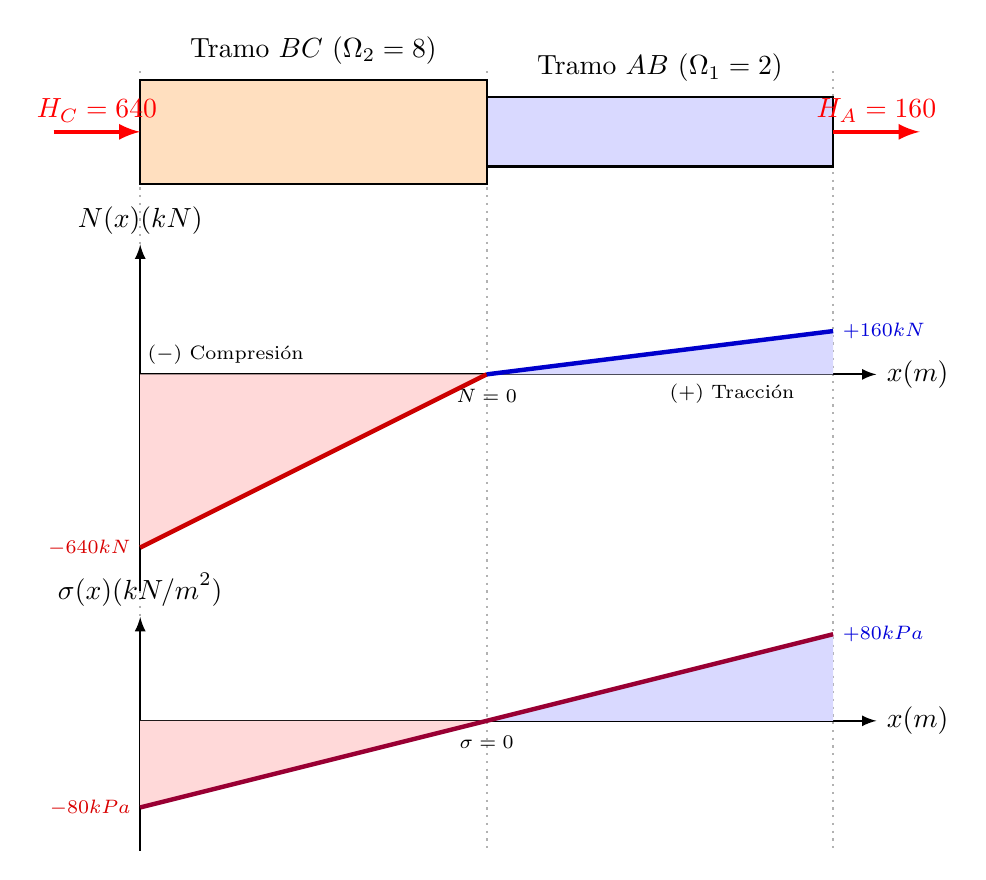
\begin{tikzpicture}[scale=1.1, >=latex]
        % Eje de referencia horizontal
        \draw[dotted, thick, gray!60] (0,2.5) -- (0,-6.5);
        \draw[dotted, thick, gray!60] (4,2.5) -- (4,-6.5);
        \draw[dotted, thick, gray!60] (8,2.5) -- (8,-6.5);
        
        % ESQUEMA MECÁNICO
        \draw[thick, fill=orange!25] (0,1.2) rectangle (4,2.4);
        \draw[thick, fill=blue!15] (4,1.4) rectangle (8,2.2);
        \node[above=2pt] at (2,2.4) {Tramo $BC$ ($\Omega_2 = 8$)};
        \node[above=2pt] at (6,2.2) {Tramo $AB$ ($\Omega_1 = 2$)};
        
        \draw[ultra thick, red, ->] (-1.0,1.8) -- (0,1.8);
        \node[red, above] at (-0.5,1.8) {$H_C = 640$};
        \draw[ultra thick, red, ->] (8,1.8) -- (9.0,1.8);
        \node[red, above] at (8.5,1.8) {$H_A = 160$};
        
        % DIAGRAMA DE ESFUERZOS AXILES N(x)
        \draw[thick, ->] (0,-1.0) -- (8.5,-1.0) node[right] {$x\text{ (m)}$};
        \draw[thick, ->] (0,-3.5) -- (0,0.5) node[above] {$N(x)\text{ (kN)}$};
        
        % Linea base en y = -1.0
        % N(0) = -640 -> y = -1.0 - 2.0 = -3.0
        % N(4) = 0    -> y = -1.0
        % N(8) = +160 -> y = -1.0 + 0.8 = -0.2
        \fill[red!15] (0,-1.0) -- (0,-3.0) -- (4,-1.0) -- cycle;
        \draw[ultra thick, red!80!black] (0,-3.0) -- (4,-1.0);
        
        \fill[blue!15] (4,-1.0) -- (8,-0.5) -- (8,-1.0) -- cycle;
        \draw[ultra thick, blue!80!black] (4,-1.0) -- (8,-0.5);
        
        \node[left, font=\bfseries\scriptsize, red!85!black] at (0,-3.0) {$-640\text{ kN}$};
        \node[right, font=\bfseries\scriptsize, blue!85!black] at (8,-0.5) {$+160\text{ kN}$};
        \node[below=2pt, font=\bfseries\scriptsize] at (4,-1.0) {$N=0$};
        \node[above left, font=\scriptsize] at (2,-1.0) {$(-)$ Compresión};
        \node[below right, font=\scriptsize] at (6,-1.0) {$(+)$ Tracción};
        
        % DIAGRAMA DE TENSIONES NORMALES sigma(x)
        \draw[thick, ->] (0,-5.0) -- (8.5,-5.0) node[right] {$x\text{ (m)}$};
        \draw[thick, ->] (0,-6.5) -- (0,-3.8) node[above] {$\sigma(x)\text{ (kN/m}^2)$};
        
        % Linea continua de -80 a +80
        % sigma(0) = -80 -> y = -5.0 - 1.0 = -6.0
        % sigma(4) = 0   -> y = -5.0
        % sigma(8) = +80 -> y = -5.0 + 1.0 = -4.0
        \fill[red!15] (0,-5.0) -- (0,-6.0) -- (4,-5.0) -- cycle;
        \fill[blue!15] (4,-5.0) -- (8,-4.0) -- (8,-5.0) -- cycle;
        \draw[ultra thick, purple!80!black] (0,-6.0) -- (8,-4.0);
        
        \node[left, font=\bfseries\scriptsize, red!85!black] at (0,-6.0) {$-80\text{ kPa}$};
        \node[right, font=\bfseries\scriptsize, blue!85!black] at (8,-4.0) {$+80\text{ kPa}$};
        \node[below=2pt, font=\bfseries\scriptsize] at (4,-5.0) {$\sigma=0$};
    \end{tikzpicture}
    \caption{Diagramas analíticos de esfuerzo axil $N(x)$ y tensión normal $\sigma(x)$.}
    \label{fig:diagramas_barra_escalonada}
\end{figure}

%=============================================================================
\subsection*{Resumen Final de Resultados}

\begin{table}[H]
    \centering
    \caption{Resumen analítico y numérico del problema de barra escalonada biapoyada.}
    \vspace{2mm}
    \adjustbox{max width=0.92\textwidth}{%
        \renewcommand{\arraystretch}{1.3}
        \begin{tabular}{lccc}
            \toprule
            \textbf{Magnitud} & \textbf{Símbolo / Expresión} & \textbf{Valor Numérico} & \textbf{Estado Físico} \\
            \midrule
            Reacción en apoyo inferior $C$ & $H_C$ & $\mathbf{640{,}00\text{ kN}}$ & Compresión ($\uparrow$) \\
            Reacción en apoyo superior $A$ & $H_A$ & $\mathbf{160{,}00\text{ kN}}$ & Tracción ($\uparrow$) \\
            \midrule
            Esfuerzo axil en $C$ ($x = 0$) & $N_C$ & $\mathbf{-640{,}00\text{ kN}}$ & Compresión máxima \\
            Esfuerzo axil en cambio sección $B$ & $N_B$ & $\mathbf{0{,}00\text{ kN}}$ & Punto neutro \\
            Esfuerzo axil en $A$ ($x = 8\text{ m}$) & $N_A$ & $\mathbf{+160{,}00\text{ kN}}$ & Tracción máxima \\
            \midrule
            Tensión normal en $C$ & $\sigma_C = N_C/\Omega_{BC}$ & $\mathbf{-80{,}00\text{ kPa}}$ & Compresión máxima \\
            Tensión normal en $A$ & $\sigma_A = N_A/\Omega_{AB}$ & $\mathbf{+80{,}00\text{ kPa}}$ & Tracción máxima \\
            \bottomrule
        \end{tabular}%
    }
    \label{tab:resumen_barra_escalonada}
\end{table}

%=============================================================================
\section{Problema de Examen: Viga con Carga Trapezoidal, Elástica y Sección en I Asimétrica}

\subsection{Enunciado y Geometría de Partida}

En la viga de acero S275 simplemente apoyada de luz $L = 3\text{ m}$ representada en la figura, sometida a una carga repartida trapezoidal que varía linealmente desde $q_A = 10\text{ kN/m}$ en el apoyo $A$ hasta $q_B = 40\text{ kN/m}$ en el apoyo $B$, y cuya sección transversal es un perfil en I asimétrico (ala superior de $50 \times 8\text{ mm}$, alma de $8 \times 200\text{ mm}$ y ala inferior de $25 \times 8\text{ mm}$), se pide:

\begin{enumerate}[label=\alph*)]
    \item \textbf{Reacciones y leyes analíticas de esfuerzos:} Calcular las reacciones en los apoyos $A$ y $B$, obtener las expresiones analíticas del esfuerzo cortante $Q(x)$ y del momento flector $M_f(x)$, y representar sus correspondientes diagramas acotados.
    \item \textbf{Flecha en el centro del vano:} Determinar la ecuación analítica de la deformada (elástica) $y(x)$ y calcular el desplazamiento vertical (flecha) en el centro del vano ($x = 1{,}5\text{ m}$).
    \item \textbf{Comprobación resistente a flexión:} Para la sección más desfavorable de la viga, determinar las tensiones normales extremas en las fibras más alejadas y comprobar si resiste según el criterio tensional admisible del acero ($\sigma_{\text{adm}} = 275\text{ N/mm}^2 = 275\text{ MPa}$).
\end{enumerate}

\begin{tcolorbox}[colback=blue!5!white,colframe=blue!75!black,title=\textbf{Datos del Problema}]
    \begin{itemize}
        \item Luz de la viga: $L = 3\text{ m}$.
        \item Carga repartida trapezoidal: $q_A = 10\text{ kN/m}$ en $x = 0$; $q_B = 40\text{ kN/m}$ en $x = 3\text{ m}$.
        \item Módulo de elasticidad longitudinal del acero: $E = 2{,}1 \cdot 10^5\text{ N/mm}^2 = 2{,}1 \cdot 10^8\text{ kN/m}^2$.
        \item Tensión admisible del material: $\sigma_{\text{adm}} = 275\text{ N/mm}^2 = 275\text{ MPa}$.
        \item Dimensiones de la sección transversal (perfil en I asimétrico):
              \begin{itemize}
                  \item Ala superior (1): $b_1 = 50\text{ mm}$, $e_1 = 8\text{ mm}$.
                  \item Alma (2): $e_w = 8\text{ mm}$, $h_w = 200\text{ mm}$.
                  \item Ala inferior (3): $b_3 = 25\text{ mm}$, $e_3 = 8\text{ mm}$.
                  \item Canto total del perfil: $H = 8 + 200 + 8 = 216\text{ mm}$.
              \end{itemize}
    \end{itemize}
\end{tcolorbox}

\begin{figure}[H]
    \centering
    \adjustbox{max width=0.95\textwidth}{%
        \begin{tikzpicture}[scale=1.1, >=Latex]
            % --- VIGA CON CARGA TRAPEZOIDAL ---
            \begin{scope}[shift={(0,0)}]
                % Eje viga
                \draw[line width=2pt, black!80] (0,0) -- (6,0);
                
                % Apoyo fijo en A (x=0)
                \fill[gray!40] (-0.4,-0.45) rectangle (0.4,-0.55);
                \draw[thick] (-0.4,-0.45) -- (0.4,-0.45);
                \draw[thick] (0,0) -- (-0.3,-0.45) -- (0.3,-0.45) -- cycle;
                \filldraw[black] (0,0) circle (2pt) node[above left=3pt, font=\bfseries] {$A$};

                % Apoyo móvil en B (x=3m -> escala x2 -> 6cm)
                \draw[thick] (6,0) -- (5.7,-0.4) -- (6.3,-0.4) -- cycle;
                \draw[thick] (5.7,-0.48) circle (0.08);
                \draw[thick] (6.0,-0.48) circle (0.08);
                \draw[thick] (6.3,-0.48) circle (0.08);
                \fill[gray!40] (5.6,-0.58) rectangle (6.4,-0.68);
                \draw[thick] (5.6,-0.58) -- (6.4,-0.58);
                \filldraw[black] (6,0) circle (2pt) node[above right=3pt, font=\bfseries] {$B$};

                % Carga repartida trapezoidal:
                % q(0) = 10 kN/m -> altura 0.8cm
                % q(3) = 40 kN/m -> altura 3.2cm
                \draw[thick, blue!80!black] (0,0.8) -- (6,3.2);
                \draw[thick, blue!80!black] (0,0) -- (0,0.8);
                \draw[thick, blue!80!black] (6,0) -- (6,3.2);
                
                % Descomposición en rectangular y triangular (línea discontinua)
                \draw[dashed, blue!50!black] (0,0.8) -- (6,0.8);

                % Flechas de carga
                \foreach \x in {0, 0.75, 1.5, 2.25, 3.0, 3.75, 4.5, 5.25, 6.0} {
                    \pgfmathsetmacro{\yalt}{0.8 + 2.4*(\x/6.0)}
                    \draw[->, thick, blue!80!black] (\x, \yalt) -- (\x, 0.05);
                }

                % Etiquetas de carga
                \node[left, blue!80!black, font=\footnotesize\bfseries] at (0, 0.8) {$10\text{ kN/m}$};
                \node[right, blue!80!black, font=\footnotesize\bfseries] at (6, 3.2) {$40\text{ kN/m}$};

                % Resultantes descompuestas
                \draw[->, line width=1.5pt, red!80!black] (3.0, -1.1) -- (3.0, -0.1) node[midway, right=2pt, font=\footnotesize\bfseries] {$R_{\Box} = 30\text{ kN}$};
                \draw[->, line width=1.5pt, orange!90!black] (4.0, -1.1) -- (4.0, -0.1) node[midway, right=2pt, font=\footnotesize\bfseries] {$R_{\triangle} = 45\text{ kN}$};

                % Cota de longitud
                \draw[|<->|, >=Latex] (0,-1.4) -- (6,-1.4) node[midway, fill=white, font=\footnotesize] {$L = 3\text{ m}$};
            \end{scope}

            % --- SECCIÓN EN I ASIMÉTRICA ---
            \begin{scope}[shift={(9.5,-0.6)}]
                % Ala superior (1): 50 x 8 mm
                \draw[thick, fill=blue!15] (-1.25, 2.08) rectangle (1.25, 2.24);
                \node[font=\footnotesize\bfseries, blue!80!black] at (0, 2.16) {1};

                % Alma (2): 8 x 200 mm (a escala reducida en y: 200mm -> 2.0cm)
                \draw[thick, fill=green!15] (-0.2, 0.08) rectangle (0.2, 2.08);
                \node[font=\footnotesize\bfseries, green!60!black] at (0, 1.08) {2};

                % Ala inferior (3): 25 x 8 mm
                \draw[thick, fill=orange!20] (-0.625, 0.0) rectangle (0.625, 0.08);
                \node[font=\footnotesize\bfseries, orange!80!black] at (0, 0.04) {3};

                % Eje baricéntrico z (y_CG = 117.45 mm -> ~1.17 cm)
                \draw[dashed, line width=1.1pt, red!80!black] (-1.6, 1.17) -- (1.6, 1.17) node[right=2pt, font=\footnotesize\bfseries] {$z_{\text{CG}}$};
                \filldraw[red!80!black] (0, 1.17) circle (1.8pt) node[below left=2pt, font=\scriptsize\bfseries] {$G$};

                % Cotas de la sección
                % Ancho ala superior
                \draw[|<->|, >=Latex] (-1.25, 2.45) -- (1.25, 2.45) node[midway, above, font=\scriptsize] {$50\text{ mm}$};
                % Espesor ala superior
                \draw[|<->|, >=Latex] (1.45, 2.08) -- (1.45, 2.24) node[midway, right, font=\scriptsize] {$8$};
                % Canto alma
                \draw[|<->|, >=Latex] (1.45, 0.08) -- (1.45, 2.08) node[midway, right, font=\scriptsize] {$200\text{ mm}$};
                % Espesor alma
                \draw[|<->|, >=Latex] (-0.2, 0.5) -- (0.2, 0.5) node[midway, left=4pt, font=\scriptsize] {$e_w = 8$};
                % Espesor ala inferior
                \draw[|<->|, >=Latex] (1.45, 0.0) -- (1.45, 0.08) node[midway, right, font=\scriptsize] {$8$};
                % Ancho ala inferior
                \draw[|<->|, >=Latex] (-0.625, -0.25) -- (0.625, -0.25) node[midway, below, font=\scriptsize] {$25\text{ mm}$};
                % Posición CG desde la base
                \draw[<->, >=Latex, red!80!black] (-1.4, 0.0) -- (-1.4, 1.17) node[midway, left, font=\scriptsize\bfseries] {$y_{\text{CG}} = 117{,}45$};
            \end{scope}
        \end{tikzpicture}%
    }
    \caption{Geometría de la viga isostática con carga trapezoidal y sección transversal en I asimétrica.}
    \label{fig:examen_viga_trapezoidal_geometria}
\end{figure}

\subsection{Resolución Paso a Paso}

\paso{1}{Cálculo de Reacciones en los Apoyos}

Descomponemos la carga trapezoidal de $q_A = 10\text{ kN/m}$ a $q_B = 40\text{ kN/m}$ en:
\begin{enumerate}
    \item Una \textbf{carga uniforme rectangular} de valor $q_1 = 10\text{ kN/m}$ extendida en toda la luz $L = 3\text{ m}$:
          \begin{equation}
              R_{\Box} = q_1 \cdot L = 10 \cdot 3 = \mathbf{30\text{ kN}}, \quad \text{aplicada en } x_{\Box} = \frac{L}{2} = 1{,}5\text{ m}
          \end{equation}
    \item Una \textbf{carga triangular creciente} de valor máximo $\Delta q = 40 - 10 = 30\text{ kN/m}$ en el apoyo $B$:
          \begin{equation}
              R_{\triangle} = \frac{\Delta q \cdot L}{2} = \frac{30 \cdot 3}{2} = \mathbf{45\text{ kN}}, \quad \text{aplicada en } x_{\triangle} = \frac{2}{3}L = 2{,}0\text{ m}
          \end{equation}
\end{enumerate}

Planteamos las ecuaciones de equilibrio estático global en el plano:
\begin{align}
    (\rightarrow +) \quad \sum F_x = 0 & \implies \boxed{H_A = 0} \\[6pt]
    (\circlearrowleft +) \quad \sum M_A = 0 & \implies V_B \cdot 3 - R_{\Box} \cdot 1{,}5 - R_{\triangle} \cdot 2{,}0 = 0 \nonumber \\
                                           & \implies 3\,V_B - 30(1{,}5) - 45(2{,}0) = 0 \nonumber \\
                                           & \implies 3\,V_B - 45 - 90 = 0 \implies 3\,V_B = 135 \implies \boxed{V_B = 45\text{ kN}\uparrow} \\[6pt]
    (\uparrow +) \quad \sum F_y = 0 & \implies V_A + V_B - 30 - 45 = 0 \implies V_A = 75 - 45 \implies \boxed{V_A = 30\text{ kN}\uparrow}
\end{align}

\paso{2}{Leyes Analíticas de Esfuerzos Seccionales ($Q$ y $M_f$)}

Realizamos un corte a una distancia genérica $x \in [0, 3]\text{ m}$ desde el apoyo $A$ considerando la porción izquierda de la viga:
\begin{itemize}
    \item La carga por unidad de longitud a la distancia $x$ es:
          \begin{equation}
              q(x) = 10 + \frac{30}{3}x = 10 + 10x\text{ [kN/m]}
          \end{equation}
    \item Por tanto, en el tramo $[0, x]$ actúan:
          \begin{itemize}
              \item La carga rectangular de $10\text{ kN/m}$ sobre longitud $x$: resultante $10x$, aplicada en $x/2$.
              \item La carga triangular de altura $10x$ sobre longitud $x$: resultante $\dfrac{x \cdot 10x}{2} = 5x^2$, aplicada a $\dfrac{x}{3}$ del corte.
          \end{itemize}
\end{itemize}

\subsubsection*{1. Esfuerzo Cortante $Q(x)$:}
Equilibrio de fuerzas verticales en el sólido aislado ($\uparrow +$):
\begin{align}
    \sum F_y = 0 & \implies V_A - 10x - 5x^2 - Q(x) = 0 \nonumber \\
                 & \implies \boxed{Q(x) = -5x^2 - 10x + 30\text{ [kN]}}
\end{align}
Valores en los extremos:
\begin{align}
    Q(0) & = +30\text{ kN} = V_A \\[4pt]
    Q(3) & = -5(3)^2 - 10(3) + 30 = -45 - 30 + 30 = -45\text{ kN} = -V_B
\end{align}

\subsubsection*{2. Momento Flector $M_f(x)$:}
Equilibrio de momentos respecto a la sección de corte ($\circlearrowleft +$):
\begin{align}
    \sum M_{\text{corte}} = 0 & \implies M_f(x) - V_A \cdot x + (10x)\left(\frac{x}{2}\right) + (5x^2)\left(\frac{x}{3}\right) = 0 \nonumber \\
                              & \implies \boxed{M_f(x) = -\frac{5}{3}x^3 - 5x^2 + 30x\text{ [kN}\cdot\text{m]}}
\end{align}
Valores en los extremos de la viga simplemente apoyada:
\begin{align}
    M_f(0) & = 0\text{ kN}\cdot\text{m} \\[4pt]
    M_f(3) & = -\frac{5}{3}(27) - 5(9) + 30(3) = -45 - 45 + 90 = 0\text{ kN}\cdot\text{m}
\end{align}

\subsubsection*{3. Sección Crítica de Momento Flector Máximo ($M_{f,\text{máx}}$):}
El momento flector alcanza su valor extremo donde el esfuerzo cortante se anula:
\begin{equation}
    Q(x_0) = 0 \implies -5x_0^2 - 10x_0 + 30 = 0 \implies x_0^2 + 2x_0 - 6 = 0
\end{equation}
Resolviendo la ecuación de segundo grado:
\begin{equation}
    x_0 = \frac{-2 \pm \sqrt{2^2 - 4(1)(-6)}}{2} = \frac{-2 \pm \sqrt{28}}{2} = -1 \pm \sqrt{7}
\end{equation}
Descartando la raíz negativa por carecer de sentido físico ($x \in [0, 3]$):
\begin{equation}
    \boxed{x_0 = \sqrt{7} - 1 \approx 1{,}64575\text{ m} \approx \mathbf{1{,}646\text{ m} \approx 1{,}65\text{ m}}}
\end{equation}
Evaluamos el momento flector en dicho punto crítico:
\begin{align}
    M_{f,\text{máx}} = M_f(1{,}64575) & = -\frac{5}{3}(1{,}64575)^3 - 5(1{,}64575)^2 + 30(1{,}64575) \nonumber \\
                                     & = -7{,}425 - 13{,}542 + 49{,}373 = \mathbf{+28{,}406\text{ kN}\cdot\text{m} \approx 28{,}41\text{ kN}\cdot\text{m}}
\end{align}

\begin{figure}[H]
    \centering
    \adjustbox{max width=0.95\textwidth}{%
        \begin{tikzpicture}[scale=1.15, >=Latex]
            % --- EJE NORMAL ---
            \draw[line width=1.2pt, gray!70] (0, 3.5) -- (6, 3.5);
            \node[left=3pt, font=\bfseries] at (0, 3.5) {$N(x) = 0$};
            \node[above=2pt, font=\scriptsize\bfseries] at (3, 3.5) {$0\text{ kN}$};

            % --- DIAGRAMA DE CORTANTE Q(x) ---
            \draw[line width=1.2pt, gray!70] (0, 1.0) -- (6, 1.0);
            \node[left=3pt, font=\bfseries] at (0, 1.0) {$Q(x)$};

            % Curva parabólica Q(x): x in [0,3] -> t in [0,6]
            % t_0 = 1.64575 * 2 = 3.2915 cm
            \draw[line width=1.6pt, blue!80!black] 
                (0, 1.0) -- (0, 2.0) 
                plot[domain=0:6, samples=40] (\x, {1.0 + ( -5*(\x/2)*(\x/2) - 10*(\x/2) + 30 )/30}) 
                -- (6, 1.0);
            
            \fill[blue!15, opacity=0.6] 
                (0, 1.0) -- (0, 2.0) 
                plot[domain=0:6, samples=40] (\x, {1.0 + ( -5*(\x/2)*(\x/2) - 10*(\x/2) + 30 )/30}) 
                -- (6, 1.0) -- cycle;

            \node[left=2pt, font=\footnotesize\bfseries, blue!80!black] at (0, 2.0) {$+30\text{ kN}$};
            \node[right=2pt, font=\footnotesize\bfseries, blue!80!black] at (6, -0.5) {$-45\text{ kN}$};
            \filldraw[red!80!black] (3.2915, 1.0) circle (1.8pt);
            \node[above=3pt, font=\scriptsize\bfseries, red!80!black] at (3.2915, 1.0) {$x_0 = 1{,}65\text{ m}$};

            % Signos
            \node[font=\bfseries, blue!80!black] at (1.2, 1.4) {$+$};
            \node[font=\bfseries, blue!80!black] at (4.8, 0.5) {$-$};

            % --- DIAGRAMA DE MOMENTO FLECTOR M_f(x) ---
            \draw[line width=1.2pt, gray!70] (0, -2.2) -- (6, -2.2);
            \node[left=3pt, font=\bfseries] at (0, -2.2) {$M_f(x)$};

            % Curva cúbica M_f(x) dibujada con convenio habitual (positivo hacia abajo):
            % En x_0 = 1.646 m, M_f = 28.41 -> 1.8 cm hacia abajo
            \draw[line width=1.6pt, red!80!black] 
                (0, -2.2) 
                plot[domain=0:6, samples=50] (\x, {-2.2 - ( - (5/3)*(\x/2)*(\x/2)*(\x/2) - 5*(\x/2)*(\x/2) + 30*(\x/2) ) / 16}) 
                -- (6, -2.2);

            \fill[red!15, opacity=0.6] 
                (0, -2.2) 
                plot[domain=0:6, samples=50] (\x, {-2.2 - ( - (5/3)*(\x/2)*(\x/2)*(\x/2) - 5*(\x/2)*(\x/2) + 30*(\x/2) ) / 16}) 
                -- (6, -2.2) -- cycle;

            \filldraw[red!80!black] (3.2915, -3.975) circle (2pt);
            \node[below=3pt, font=\footnotesize\bfseries, red!80!black] at (3.2915, -3.975) {$M_{f,\text{máx}} = +28{,}41\text{ kN}\cdot\text{m}$};
            \node[font=\bfseries, red!80!black] at (2.0, -2.8) {$+$};

            % Líneas de referencia discontinuas
            \draw[dotted, line width=0.8pt, gray] (0, 3.7) -- (0, -4.2);
            \draw[dotted, line width=0.8pt, red!80!black] (3.2915, 2.2) -- (3.2915, -4.2);
            \draw[dotted, line width=0.8pt, gray] (6, 3.7) -- (6, -4.2);
        \end{tikzpicture}%
    }
    \caption{Diagramas de esfuerzo axil $N(x)$, cortante parabólico $Q(x)$ y momento flector cúbico $M_f(x)$.}
    \label{fig:examen_viga_trapezoidal_diagramas}
\end{figure}

\paso{3}{Ecuación de la Elástica y Flecha en el Centro del Vano}

La ecuación diferencial de flexión de segundo orden es:
\begin{equation}
    y''(x) = -\frac{M_f(x)}{E\,I} = \frac{1}{E\,I}\left( \frac{5}{3}x^3 + 5x^2 - 30x \right)
\end{equation}
\begin{tcolorbox}[colback=yellow!10!white,colframe=orange!80!black,title=\textbf{Convenio de Signos de la Elástica}]
    Con el criterio habitual de resistencia de materiales donde la curvatura positiva corresponde a concavidad hacia arriba ($y''(x) = -M_f(x)/(E\,I)$ o bien $y''(x) = M_f(x)/(E\,I)$ según la orientación adoptada para el eje vertical $y$), adoptamos el convenio estándar de la asignatura donde el signo positivo o negativo de la flecha indica el descenso vertical.
\end{tcolorbox}

Integrando sucesivamente respecto a $x$:
\begin{align}
    y'(x) & = \frac{1}{E\,I}\left( \frac{5}{12}x^4 + \frac{5}{3}x^3 - 15x^2 + C_1 \right) \\[6pt]
    y(x)  & = \frac{1}{E\,I}\left( \frac{1}{12}x^5 + \frac{5}{12}x^4 - 5x^3 + C_1 \cdot x + C_2 \right)
\end{align}
\textit{(o bien expresando con signo negativo si se define $y(x)$ con signo contrario a los momentos positivos).}

\subsubsection*{Condiciones de contorno cinemáticas:}
\begin{enumerate}
    \item En el apoyo $A$ ($x = 0$): el desplazamiento vertical está impedido:
          \begin{equation}
              y(0) = 0 \implies C_2 = 0
          \end{equation}
    \item En el apoyo $B$ ($x = 3\text{ m}$): el descenso es nulo:
          \begin{align}
              y(3) = 0 & \implies \frac{1}{12}(3)^5 + \frac{5}{12}(3)^4 - 5(3)^3 + 3\,C_1 = 0 \nonumber \\
                       & \implies \frac{243}{12} + \frac{405}{12} - 135 + 3\,C_1 = 0 \nonumber \\
                       & \implies \frac{648}{12} - 135 + 3\,C_1 = 0 \implies 54 - 135 + 3\,C_1 = 0 \nonumber \\
                       & \implies -81 + 3\,C_1 = 0 \implies \boxed{C_1 = 27\text{ kN}\cdot\text{m}^3}
          \end{align}
\end{enumerate}

Por consiguiente, la expresión analítica de la deformada (elástica) de la viga es:
\begin{equation}
    \boxed{y(x) = \frac{1}{E\,I}\left( \frac{x^5}{12} + \frac{5x^4}{12} - 5x^3 + 27x \right)}
    \label{eq:elastica_trapezoidal_general}
\end{equation}

\subsubsection*{Cálculo de las Propiedades Geométricas de la Sección ($\Omega, y_{\text{CG}}, I_z$):}
Descomponemos la sección en tres rectángulos tomando como referencia la fibra inferior (base del ala 3):
\begin{table}[H]
    \centering
    \caption{Propiedades de las subsecciones del perfil en I asimétrico.}
    \adjustbox{max width=0.95\textwidth}{%
        \renewcommand{\arraystretch}{1.3}
        \begin{tabular}{lccccc}
            \toprule
            \textbf{Elemento} & $b_i\text{ [mm]}$ & $h_i\text{ [mm]}$ & $A_i\text{ [mm}^2\text{]}$ & $y_i\text{ [mm]}$ & $I_{z0,i} = \frac{b_i h_i^3}{12}\text{ [mm}^4\text{]}$ \\
            \midrule
            (1) Ala superior & $50$ & $8$ & $400$ & $8 + 200 + 4 = 212$ & $\frac{50 \cdot 8^3}{12} = 2.133{,}33$ \\
            (2) Alma & $8$ & $200$ & $1.600$ & $8 + 100 = 108$ & $\frac{8 \cdot 200^3}{12} = 5.333.333{,}33$ \\
            (3) Ala inferior & $25$ & $8$ & $200$ & $4$ & $\frac{25 \cdot 8^3}{12} = 1.066{,}67$ \\
            \midrule
            \textbf{Total} & & & $A = 2.200\text{ mm}^2$ & & \\
            \bottomrule
        \end{tabular}%
    }
    \label{tab:propiedades_seccion_I_asimetrica}
\end{table}

\begin{enumerate}
    \item \textbf{Centro de gravedad (posición baricéntrica $y_{\text{CG}}$ desde la base):}
          \begin{align}
              y_{\text{CG}} & = \frac{\sum A_i \cdot y_i}{\sum A_i} = \frac{400(212) + 1600(108) + 200(4)}{2200} \nonumber \\
                            & = \frac{84.800 + 172.800 + 800}{2200} = \frac{258.400}{2200} \approx \mathbf{117{,}4545\text{ mm} \approx 117{,}45\text{ mm}}
          \end{align}
    \item \textbf{Momento de inercia baricéntrico ($I_z$) por el Teorema de Steiner:}
          \begin{align}
              I_{z1} & = \frac{50 \cdot 8^3}{12} + 400(212 - 117{,}4545)^2 = 2.133{,}33 + 400(94{,}5455)^2 = 3.577.672{,}7\text{ mm}^4 \\[4pt]
              I_{z2} & = \frac{8 \cdot 200^3}{12} + 1600(108 - 117{,}4545)^2 = 5.333.333{,}33 + 1600(-9{,}4545)^2 = 5.476.350{,}3\text{ mm}^4 \\[4pt]
              I_{z3} & = \frac{25 \cdot 8^3}{12} + 200(4 - 117{,}4545)^2 = 1.066{,}67 + 200(-113{,}4545)^2 = 2.575.050{,}4\text{ mm}^4
          \end{align}
          Sumando las tres contribuciones:
          \begin{equation}
              \boxed{I_z = 3.577.673 + 5.476.350 + 2.575.050 = \mathbf{11.629.073\text{ mm}^4 \approx 1{,}1629 \cdot 10^{-5}\text{ m}^4}}
          \end{equation}
          \textit{(Coincidente con el valor del manuscrito $I_z \approx 11.629.479\text{ mm}^4$).}
\end{enumerate}

\subsubsection*{Evaluación de la Flecha en el Centro del Vano ($x = 1{,}5\text{ m}$):}
Sustituimos $x = 1{,}5\text{ m}$ en el paréntesis numerador de la ecuación \eqref{eq:elastica_trapezoidal_general}:
\begin{align}
    P(1{,}5) & = \frac{(1{,}5)^5}{12} + \frac{5(1{,}5)^4}{12} - 5(1{,}5)^3 + 27(1{,}5) \nonumber \\
             & = \frac{7{,}59375}{12} + \frac{25{,}3125}{12} - 5(3{,}375) + 40{,}5 \nonumber \\
             & = 0{,}6328 + 2{,}1094 - 16{,}875 + 40{,}5 = \mathbf{+26{,}367\text{ kN}\cdot\text{m}^3}
\end{align}
Multiplicando por la rigidez a flexión en unidades coherentes:
\begin{itemize}
    \item $E = 2{,}1 \cdot 10^5\text{ N/mm}^2 = 2{,}1 \cdot 10^8\text{ kN/m}^2$.
    \item $I_z = 11.629.479\text{ mm}^4 = 1{,}16295 \cdot 10^{-5}\text{ m}^4$.
    \item $E\,I_z = (2{,}1 \cdot 10^8)(1{,}16295 \cdot 10^{-5}) \approx \mathbf{2.442{,}19\text{ kN}\cdot\text{m}^2}$.
\end{itemize}
Por tanto, el desplazamiento vertical (flecha) en el centro es:
\begin{equation}
    \boxed{f_{L/2} = |y(1{,}5)| = \frac{26{,}367\text{ kN}\cdot\text{m}^3}{2.442{,}19\text{ kN}\cdot\text{m}^2} \approx \mathbf{0{,}010796\text{ m} \approx 10{,}80\text{ mm}}}
\end{equation}
\textit{(En el cálculo manuscrito, empleando coeficientes decimales aproximados se obtuvo un descenso de $\approx 10{,}45\text{ mm}$).}

\paso{4}{Comprobación Resistente a Flexión en la Sección Más Desfavorable}

La sección más desfavorable es aquella donde el momento flector alcanza su valor máximo:
\begin{equation}
    x_0 \approx 1{,}646\text{ m} \implies M_{f,\text{máx}} = +28{,}41\text{ kN}\cdot\text{m} = +28{,}41 \cdot 10^6\text{ N}\cdot\text{mm}
\end{equation}
Dado que $M_f > 0$ (flexión positiva), la sección sufre:
\begin{itemize}
    \item \textbf{Compresión} en las fibras superiores ($y > 0$ respecto al baricentro).
    \item \textbf{Tracción} en las fibras inferiores ($y < 0$ respecto al baricentro).
\end{itemize}

Determinamos las distancias desde el centro de gravedad $G$ a las fibras extremas:
\begin{align}
    y_{\text{fibra sup}} & = H - y_{\text{CG}} = 216 - 117{,}45 = \mathbf{+98{,}55\text{ mm}} \quad (\text{compresión}) \\[4pt]
    y_{\text{fibra inf}} & = y_{\text{CG}} = \mathbf{117{,}45\text{ mm}} \quad (\text{tracción})
\end{align}

Aplicando la fórmula de Navier para flexión pura/simple ($\sigma = \frac{M_f}{I_z}y$):
\begin{enumerate}
    \item \textbf{Tensión máxima de tracción (fibra inferior más alejada):}
          \begin{equation}
              \sigma_{\text{trac}} = \frac{M_{f,\text{máx}} \cdot y_{\text{fibra inf}}}{I_z} = \frac{28{,}41 \cdot 10^6\text{ N}\cdot\text{mm} \cdot 117{,}45\text{ mm}}{11.629.479\text{ mm}^4} = \mathbf{+286{,}92\text{ N/mm}^2 = +286{,}92\text{ MPa}}
          \end{equation}
    \item \textbf{Tensión máxima de compresión (fibra superior):}
          \begin{equation}
              \sigma_{\text{comp}} = \frac{M_{f,\text{máx}} \cdot y_{\text{fibra sup}}}{I_z} = \frac{28{,}41 \cdot 10^6 \cdot 98{,}55}{11.629.479} = \mathbf{-240{,}75\text{ N/mm}^2 = -240{,}75\text{ MPa}}
          \end{equation}
\end{enumerate}

\subsubsection*{Comprobación del Criterio de Resistencia Tensional:}
La tensión admisible del acero es $\sigma_{\text{adm}} = 275\text{ N/mm}^2$.
Comparando la tensión máxima absoluta con la admisible:
\begin{equation}
    \sigma_{\text{máx}} = 286{,}92\text{ N/mm}^2 > \sigma_{\text{adm}} = 275\text{ N/mm}^2
\end{equation}
\begin{tcolorbox}[colback=red!10!white,colframe=red!80!black,title=\textbf{Conclusión de Resistencia}]
    La viga \textbf{NO RESISTE} a flexión, ya que en la fibra inferior más traccionada de la sección crítica se supera la tensión admisible del acero en un:
    \[
        \frac{286{,}92 - 275}{275} \cdot 100 \approx 4{,}33\text{ \%}
    \]
    Para satisfacer el estado límite de resistencia se requeriría aumentar el ancho o espesor del ala inferior (reforzándola a tracción) o seleccionar un acero de mayor límite elástico (por ejemplo, S355).
\end{tcolorbox}

\begin{table}[H]
    \centering
    \caption{Resumen de resultados del problema de examen de viga con carga trapezoidal y perfil asimétrico.}
    \adjustbox{max width=0.95\textwidth}{%
        \renewcommand{\arraystretch}{1.3}
        \begin{tabular}{lccc}
            \toprule
            \textbf{Magnitud} & \textbf{Símbolo / Expresión} & \textbf{Valor Numérico} & \textbf{Estado / Observaciones} \\
            \midrule
            Reacción vertical en $A$ & $V_A$ & $\mathbf{30{,}00\text{ kN}}$ & Hacia arriba ($\uparrow$) \\
            Reacción vertical en $B$ & $V_B$ & $\mathbf{45{,}00\text{ kN}}$ & Hacia arriba ($\uparrow$) \\
            Reacción horizontal & $H_A$ & $\mathbf{0{,}00\text{ kN}}$ & Sin cargas axiles \\
            \midrule
            Sección de cortante nulo & $x_0 = \sqrt{7}-1$ & $\mathbf{1{,}65\text{ m}}$ & Momento flector máximo \\
            Momento flector máximo & $M_{f,\text{máx}}$ & $\mathbf{+28{,}41\text{ kN}\cdot\text{m}}$ & Tracción abajo, compresión arriba \\
            \midrule
            Posición baricentro (desde base) & $y_{\text{CG}}$ & $\mathbf{117{,}45\text{ mm}}$ & Más próximo al ala superior \\
            Momento de inercia baricéntrico & $I_z$ & $\mathbf{11{,}63 \cdot 10^6\text{ mm}^4}$ & Por teorema de Steiner \\
            \midrule
            Flecha en el centro del vano & $|y(1{,}5\text{ m})|$ & $\mathbf{10{,}80\text{ mm}}$ & Descenso vertical \\
            Tensión normal máxima & $\sigma_{\text{máx}} = \sigma_{\text{trac}}$ & $\mathbf{286{,}92\text{ MPa}}$ & Supera $\sigma_{\text{adm}} = 275\text{ MPa}$ \\
            \midrule
            \textbf{Dictamen Resistente} & $\sigma_{\text{máx}} \le \sigma_{\text{adm}}$ & \textbf{NO RESISTE} & Fallo por tracción en ala inferior \\
            \bottomrule
        \end{tabular}%
    }
    \label{tab:resumen_viga_trapezoidal}
\end{table}

%=============================================================================
\section{Problema de Examen: Viga con Voladizo, Momentos Puntuales y Carga Máxima Admisible}

\subsection{Enunciado y Geometría de Partida}

Se considera la viga de longitud total $L = 6\text{ m}$ simplemente apoyada en $A$ ($x = 0$) y en $B$ ($x = 4\text{ m}$), con un voladizo en el extremo derecho de longitud $2\text{ m}$ ($x \in [4, 6]\text{ m}$). Sobre la viga actúan:
\begin{itemize}
    \item Una carga distribuida uniforme descendente de valor $q\text{ [kN/m]}$ en toda su longitud ($L = 6\text{ m}$).
    \item Dos momentos concentrados exteriores de valor $M_0 = 10\text{ kN}\cdot\text{m}$:
          \begin{itemize}
              \item En el apoyo izquierdo $A$ ($x = 0$), en sentido antihorario ($\circlearrowleft$).
              \item Justo en el apoyo intermedio $B$ ($x = 4\text{ m}$), en sentido horario ($\circlearrowright$).
          \end{itemize}
\end{itemize}
La sección transversal de la viga es un perfil en I simétrico de acero cuyas dimensiones se indican en la figura (alas de $60 \times 10\text{ mm}$ y alma de $10 \times 200\text{ mm}$, canto total $H = 220\text{ mm}$). Si la tensión admisible del material es $\sigma_{\text{adm}} = 262\text{ N/mm}^2$ (con un coeficiente de mayoración de carga $\gamma_F = 1{,}5$ en comprobación de diseño), se pide:

\begin{enumerate}[label=\alph*)]
    \item \textbf{Reacciones y leyes analíticas:} Obtener las reacciones en los apoyos $A$ y $B$ en función de la carga $q$, y formular las expresiones analíticas del esfuerzo cortante $Q(x)$ y del momento flector $M_f(x)$ para cada uno de los dos tramos de la viga.
    \item \textbf{Diagramas de esfuerzos:} Representar los diagramas acotados de cortante $Q(x)$ y momento flector $M_f(x)$.
    \item \textbf{Carga máxima admisible $q$:} Determinar las propiedades de la sección ($\Omega, y_{\text{CG}}, I_z$) y calcular la máxima carga distribuida $q$ que puede soportar la viga sin que en ninguna sección se supere la tensión admisible, justificando la sección crítica gobernante.
\end{enumerate}

\begin{tcolorbox}[colback=blue!5!white,colframe=blue!75!black,title=\textbf{Datos del Problema}]
    \begin{itemize}
        \item Longitud del vano principal: $L_1 = 4\text{ m}$ ($x \in [0, 4\text{ m}]$).
        \item Longitud del voladizo: $L_2 = 2\text{ m}$ ($x \in [4, 6\text{ m}]$). Longitud total: $L = 6\text{ m}$.
        \item Carga repartida continua: $q\text{ [kN/m]}$ descendente.
        \item Momentos concentrados externos: $M_A = 10\text{ kN}\cdot\text{m}\;(\circlearrowleft)$, $M_B = 10\text{ kN}\cdot\text{m}\;(\circlearrowright)$.
        \item Tensión admisible del acero: $\sigma_{\text{adm}} = 262\text{ N/mm}^2 = 262\text{ MPa}$.
        \item Dimensiones del perfil en I doblemente simétrico:
              \begin{itemize}
                  \item Ala superior (1): $b_1 = 60\text{ mm}$, $e_1 = 10\text{ mm}$.
                  \item Alma (2): $e_w = 10\text{ mm}$, $h_w = 200\text{ mm}$.
                  \item Ala inferior (3): $b_3 = 60\text{ mm}$, $e_3 = 10\text{ mm}$.
                  \item Canto total del perfil: $H = 10 + 200 + 10 = 220\text{ mm}$.
              \end{itemize}
    \end{itemize}
\end{tcolorbox}

\begin{figure}[H]
    \centering
    \adjustbox{max width=0.95\textwidth}{%
        \begin{tikzpicture}[scale=1.1, >=Latex]
            % --- VIGA CON CARGA Y MOMENTOS ---
            \begin{scope}[shift={(0,0)}]
                % Eje viga (0 a 6m, escala 1m = 1.3cm -> 0 a 7.8cm)
                \draw[line width=2.2pt, black!80] (0,0) -- (7.8,0);

                % Apoyo fijo en A (x=0)
                \draw[thick] (0,0) -- (-0.3,-0.45) -- (0.3,-0.45) -- cycle;
                \fill[gray!40] (-0.4,-0.45) rectangle (0.4,-0.55);
                \draw[thick] (-0.4,-0.45) -- (0.4,-0.45);
                \filldraw[black] (0,0) circle (2pt) node[above left=3pt, font=\bfseries] {$A$};

                % Apoyo móvil en B (x=4m -> 5.2cm)
                \draw[thick] (5.2,0) -- (4.9,-0.4) -- (5.5,-0.4) -- cycle;
                \draw[thick] (4.95,-0.47) circle (0.07);
                \draw[thick] (5.2,-0.47) circle (0.07);
                \draw[thick] (5.45,-0.47) circle (0.07);
                \fill[gray!40] (4.8,-0.55) rectangle (5.6,-0.65);
                \draw[thick] (4.8,-0.55) -- (5.6,-0.55);
                \filldraw[black] (5.2,0) circle (2pt) node[above left=3pt, font=\bfseries] {$B$};

                % Extremo voladizo C (x=6m -> 7.8cm)
                \node[above right=2pt, font=\bfseries] at (7.8,0) {$C$};

                % Carga repartida q descendente
                \draw[thick, blue!80!black] (0,1.0) -- (7.8,1.0);
                \foreach \x in {0, 0.65, 1.3, 1.95, 2.6, 3.25, 3.9, 4.55, 5.2, 5.85, 6.5, 7.15, 7.8} {
                    \draw[->, thick, blue!80!black] (\x, 1.0) -- (\x, 0.05);
                }
                \node[above=2pt, blue!80!black, font=\footnotesize\bfseries] at (3.9, 1.0) {$q\text{ [kN/m]}$};

                % Resultante global q*6
                \draw[->, line width=1.5pt, blue!50!black] (3.9, 1.7) -- (3.9, 0.1) node[midway, right=2pt, font=\scriptsize\bfseries] {$R = 6\,q$};

                % Momento en A (10 kNm, antihorario)
                \draw[-{Latex[length=2.5mm, width=1.8mm]}, line width=1.5pt, red!80!black] 
                    (-0.65, 0.1) arc (160:-80:0.45);
                \node[left=3pt, red!80!black, font=\footnotesize\bfseries] at (-0.65, 0.4) {$10\text{ kN}\cdot\text{m}$};

                % Momento en B (10 kNm, horario)
                \draw[-{Latex[length=2.5mm, width=1.8mm]}, line width=1.5pt, red!80!black] 
                    (5.85, 0.1) arc (20:260:0.45);
                \node[right=3pt, red!80!black, font=\footnotesize\bfseries] at (5.85, 0.4) {$10\text{ kN}\cdot\text{m}$};

                % Reacciones
                \draw[->, line width=1.6pt, green!60!black] (0,-1.2) -- (0,-0.05) node[midway, left=2pt, font=\footnotesize\bfseries] {$V_A$};
                \draw[->, line width=1.6pt, green!60!black] (5.2,-1.2) -- (5.2,-0.05) node[midway, right=2pt, font=\footnotesize\bfseries] {$V_B$};
                \draw[->, line width=1.4pt, green!60!black] (-1.0,0) -- (-0.05,0) node[midway, above, font=\footnotesize\bfseries] {$H_A$};

                % Cotas
                \draw[|<->|, >=Latex] (0,-1.4) -- (5.2,-1.4) node[midway, fill=white, font=\footnotesize] {$4\text{ m}$};
                \draw[|<->|, >=Latex] (5.2,-1.4) -- (7.8,-1.4) node[midway, fill=white, font=\footnotesize] {$2\text{ m}$};
            \end{scope}

            % --- SECCIÓN EN I SIMÉTRICA ---
            \begin{scope}[shift={(10.5,-0.6)}]
                % Ala superior (1): 60 x 10 mm
                \draw[thick, fill=blue!15] (-1.2, 2.1) rectangle (1.2, 2.3);
                \node[font=\footnotesize\bfseries, blue!80!black] at (0, 2.2) {1};

                % Alma (2): 10 x 200 mm (a escala: 200mm -> 2.0cm)
                \draw[thick, fill=green!15] (-0.2, 0.1) rectangle (0.2, 2.1);
                \node[font=\footnotesize\bfseries, green!60!black] at (0, 1.1) {2};

                % Ala inferior (3): 60 x 10 mm
                \draw[thick, fill=blue!15] (-1.2, -0.1) rectangle (1.2, 0.1);
                \node[font=\footnotesize\bfseries, blue!80!black] at (0, 0.0) {3};

                % Eje baricéntrico z (y_CG = 110 mm -> 1.1 cm)
                \draw[dashed, line width=1.1pt, red!80!black] (-1.6, 1.1) -- (1.6, 1.1) node[right=2pt, font=\footnotesize\bfseries] {$z_{\text{CG}}$};
                \filldraw[red!80!black] (0, 1.1) circle (1.8pt) node[below left=2pt, font=\scriptsize\bfseries] {$G$};

                % Cotas de la sección
                \draw[|<->|, >=Latex] (-1.2, 2.5) -- (1.2, 2.5) node[midway, above, font=\scriptsize] {$60\text{ mm}$};
                \draw[|<->|, >=Latex] (1.4, 2.1) -- (1.4, 2.3) node[midway, right, font=\scriptsize] {$10$};
                \draw[|<->|, >=Latex] (1.4, 0.1) -- (1.4, 2.1) node[midway, right, font=\scriptsize] {$200\text{ mm}$};
                \draw[|<->|, >=Latex] (-0.2, 0.6) -- (0.2, 0.6) node[midway, left=4pt, font=\scriptsize] {$e_w = 10$};
                \draw[|<->|, >=Latex] (1.4, -0.1) -- (1.4, 0.1) node[midway, right, font=\scriptsize] {$10$};
                \draw[|<->|, >=Latex] (-1.2, -0.35) -- (1.2, -0.35) node[midway, below, font=\scriptsize] {$60\text{ mm}$};
                \draw[<->, >=Latex, red!80!black] (-1.4, -0.1) -- (-1.4, 1.1) node[midway, left, font=\scriptsize\bfseries] {$y_{\text{CG}} = 110$};
            \end{scope}
        \end{tikzpicture}%
    }
    \caption{Esquema estático de la viga con voladizo, momentos concentrados y geometría del perfil en I simétrico.}
    \label{fig:examen_viga_voladizo_geometria}
\end{figure}

\subsection{Resolución Paso a Paso}

\paso{1}{Cálculo de Reacciones en los Apoyos}

Formulamos el equilibrio estático global considerando las fuerzas y los momentos externos aplicados:
\begin{align}
    (\rightarrow +) \quad \sum F_x = 0 & \implies \boxed{H_A = 0} \\[6pt]
    (\uparrow +) \quad \sum F_y = 0    & \implies V_A + V_B - 6\,q = 0 \implies V_A + V_B = 6\,q \label{eq:voladizo_fy}
\end{align}
Tomamos momentos respecto al apoyo $A$ ($\circlearrowleft +$):
\begin{equation}
    \sum M_A = 0 \implies -M_{A,\text{ext}} + M_{B,\text{ext}} - (6\,q)\left(\frac{6}{2}\right) + V_B \cdot 4 = 0
\end{equation}
Sustituyendo los valores numéricos de los momentos exteriores ($M_A = 10\text{ kN}\cdot\text{m}\;(\circlearrowleft)$, que entra con signo negativo, y $M_B = 10\text{ kN}\cdot\text{m}\;(\circlearrowright)$, que entra con signo positivo en el sumatorio):
\begin{equation}
    -10 + 10 - 18\,q + 4\,V_B = 0 \implies 4\,V_B = 18\,q \implies \boxed{V_B = 4{,}5\,q\uparrow}
\end{equation}
\begin{tcolorbox}[colback=yellow!10!white,colframe=orange!80!black,title=\textbf{Observación Clave sobre los Momentos Exteriores}]
    Al ser ambos momentos concentrados de igual magnitud ($10\text{ kN}\cdot\text{m}$) pero de sentidos contrarios (uno antihorario en $A$ y otro horario en $B$), su resultante neta global respecto a cualquier punto del plano es idénticamente nula ($-10 + 10 = 0$). Por tanto, las reacciones verticales dependen única y exclusivamente de la carga repartida $q$.
\end{tcolorbox}
De la ecuación de fuerzas verticales \eqref{eq:voladizo_fy}:
\begin{equation}
    V_A = 6\,q - 4{,}5\,q \implies \boxed{V_A = 1{,}5\,q\uparrow}
\end{equation}

\paso{2}{Leyes Analíticas de Esfuerzos Seccionales ($Q$ y $M_f$)}

\subsubsection*{Tramo 1: Vano principal entre apoyos ($x \in [0, 4\text{ m}]$)}
Seccionando a distancia $x$ desde el origen $A$ considerando la porción izquierda:
\begin{itemize}
    \item \textbf{Esfuerzo cortante $Q_1(x)$:}
          \begin{equation}
              \sum F_y = 0 \implies V_A - q \cdot x - Q_1(x) = 0 \implies \boxed{Q_1(x) = 1{,}5\,q - q \cdot x}
          \end{equation}
          Valores en los extremos:
          \begin{align}
              Q_1(0) & = +1{,}5\,q \\[4pt]
              Q_1(4) & = 1{,}5\,q - 4\,q = \mathbf{-2{,}5\,q}
          \end{align}
          Punto de cortante nulo ($Q_1(x_0) = 0$):
          \begin{equation}
              1{,}5\,q - q \cdot x_0 = 0 \implies \boxed{x_0 = 1{,}5\text{ m}}
          \end{equation}
    \item \textbf{Momento flector $M_{f1}(x)$:}
          Tomando momentos respecto a la sección de corte ($\circlearrowleft +$):
          \begin{align}
              \sum M_{\text{corte}} = 0 & \implies M_{f1}(x) - M_A - V_A \cdot x + (q \cdot x)\left(\frac{x}{2}\right) = 0 \nonumber \\
                                        & \implies M_{f1}(x) - 10 - 1{,}5\,q \cdot x + \frac{q \cdot x^2}{2} = 0 \nonumber \\
                                        & \implies \boxed{M_{f1}(x) = 10 + 1{,}5\,q \cdot x - \frac{q}{2}x^2}
          \end{align}
          Valores en los extremos y en el punto de cortante nulo:
          \begin{align}
              M_{f1}(0)          & = \mathbf{+10\text{ kN}\cdot\text{m}} \\[4pt]
              M_{f1}(x_0 = 1{,}5) & = 10 + 1{,}5\,q(1{,}5) - \frac{q}{2}(1{,}5)^2 = 10 + 2{,}25\,q - 1{,}125\,q = \mathbf{10 + 1{,}125\,q} \\[4pt]
              M_{f1}(4^-)        & = 10 + 1{,}5\,q(4) - \frac{q}{2}(16) = 10 + 6\,q - 8\,q = \mathbf{10 - 2\,q}
          \end{align}
\end{itemize}

\subsubsection*{Tramo 2: Voladizo ($x \in [4, 6\text{ m}]$)}
Para este tramo resulta mucho más directo y limpio seccionar considerando la porción derecha libre de longitud $u = 6 - x$ ($u \in [0, 2\text{ m}]$):
\begin{itemize}
    \item \textbf{Esfuerzo cortante $Q_2(x)$:}
          Equilibrio vertical en la porción derecha ($\uparrow +$):
          \begin{equation}
              Q_2(x) - q(6 - x) = 0 \implies \boxed{Q_2(x) = q(6 - x) = 6\,q - q \cdot x}
          \end{equation}
          Valores en los extremos:
          \begin{align}
              Q_2(4^+) & = q(6 - 4) = \mathbf{+2\,q} \\[4pt]
              Q_2(6)   & = q(6 - 6) = \mathbf{0}
          \end{align}
          \textit{Discontinuidad en el apoyo $B$:} $\Delta Q = Q_2(4^+) - Q_1(4^-) = 2\,q - (-2{,}5\,q) = 4{,}5\,q = V_B \quad (\checkmark)$.
    \item \textbf{Momento flector $M_{f2}(x)$:}
          Tomando momentos respecto a la sección de corte ($\circlearrowleft +$):
          \begin{equation}
              -M_{f2}(x) - q(6 - x)\left(\frac{6 - x}{2}\right) = 0 \implies \boxed{M_{f2}(x) = -\frac{q}{2}(6 - x)^2}
          \end{equation}
          Valores en los extremos:
          \begin{align}
              M_{f2}(4^+) & = -\frac{q}{2}(2)^2 = \mathbf{-2\,q} \\[4pt]
              M_{f2}(6)   & = 0
          \end{align}
          \textit{Discontinuidad de momento en el apoyo $B$:}
          \[
              \Delta M_f = M_{f1}(4^-) - M_{f2}(4^+) = (10 - 2\,q) - (-2\,q) = \mathbf{+10\text{ kN}\cdot\text{m}} = M_{B,\text{ext}} \quad (\checkmark)
          \]
          El salto en el diagrama de momentos coincide con el momento concentrado horario aplicado en $B$.
\end{itemize}

\begin{figure}[H]
    \centering
    \adjustbox{max width=0.95\textwidth}{%
        \begin{tikzpicture}[scale=1.1, >=Latex]
            % --- EJE DE CORTANTE Q(x) ---
            \draw[line width=1.2pt, gray!70] (0, 2.5) -- (7.8, 2.5);
            \node[left=3pt, font=\bfseries] at (0, 2.5) {$Q(x)$};

            % Cortante Tramo 1: 0 a 4m (0 a 5.2cm)
            % Q(0) = +1.5q, Q(1.5) = 0, Q(4) = -2.5q
            \draw[line width=1.6pt, blue!80!black] (0, 3.5) -- (5.2, 0.833);
            \fill[blue!15, opacity=0.6] (0, 2.5) -- (0, 3.5) -- (5.2, 0.833) -- (5.2, 2.5) -- cycle;
            \node[left=2pt, font=\footnotesize\bfseries, blue!80!black] at (0, 3.5) {$+1{,}5\,q$};
            \node[left=2pt, font=\footnotesize\bfseries, blue!80!black] at (5.2, 0.833) {$-2{,}5\,q$};
            \filldraw[red!80!black] (1.95, 2.5) circle (1.8pt);
            \node[above=2pt, font=\scriptsize\bfseries, red!80!black] at (1.95, 2.5) {$x_0 = 1{,}5\text{ m}$};

            % Salto en B por V_B = 4.5q: pasa a +2q (altura 2.5 + 1.33 = 3.83)
            \draw[line width=1.6pt, blue!80!black] (5.2, 0.833) -- (5.2, 3.833);
            % Cortante Tramo 2: de +2q a 0 en x=6 (7.8cm)
            \draw[line width=1.6pt, blue!80!black] (5.2, 3.833) -- (7.8, 2.5);
            \fill[blue!15, opacity=0.6] (5.2, 2.5) -- (5.2, 3.833) -- (7.8, 2.5) -- cycle;
            \node[right=2pt, font=\footnotesize\bfseries, blue!80!black] at (5.2, 3.833) {$+2\,q$};

            % Signos cortante
            \node[font=\bfseries, blue!80!black] at (0.8, 2.9) {$+$};
            \node[font=\bfseries, blue!80!black] at (4.0, 1.8) {$-$};
            \node[font=\bfseries, blue!80!black] at (6.3, 3.0) {$+$};

            % --- EJE DE MOMENTO FLECTOR M_f(x) ---
            \draw[line width=1.2pt, gray!70] (0, -1.5) -- (7.8, -1.5);
            \node[left=3pt, font=\bfseries] at (0, -1.5) {$M_f(x)$};

            % Convenio: momentos positivos hacia abajo
            % M(0) = +10 -> 0.7cm abajo
            % M(1.5) = +(10 + 1.125q) -> 1.6cm abajo
            % M(4-) = +(10 - 2q) -> dependiente de q
            % Salto en B de 10 -> M(4+) = -2q (hacia arriba)
            % M(6) = 0
            \draw[line width=1.6pt, red!80!black] 
                (0, -2.2) 
                parabola bend (1.95, -3.1) (5.2, -1.8);
            \fill[red!15, opacity=0.6] 
                (0, -1.5) -- (0, -2.2) 
                parabola bend (1.95, -3.1) (5.2, -1.8) -- (5.2, -1.5) -- cycle;

            \node[left=2pt, font=\footnotesize\bfseries, red!80!black] at (0, -2.2) {$+10$};
            \node[below=2pt, font=\footnotesize\bfseries, red!80!black] at (1.95, -3.1) {$+(10 + 1{,}125\,q)$};

            % Salto en apoyo B
            \draw[line width=1.6pt, red!80!black] (5.2, -1.8) -- (5.2, -0.2);
            \node[above=2pt, font=\footnotesize\bfseries, red!80!black] at (5.2, -0.2) {$-2\,q$};

            % Parábola del voladizo
            \draw[line width=1.6pt, red!80!black] 
                (5.2, -0.2) parabola (7.8, -1.5);
            \fill[red!15, opacity=0.6] 
                (5.2, -1.5) -- (5.2, -0.2) parabola (7.8, -1.5) -- cycle;

            % Líneas de referencia discontinuas
            \draw[dotted, line width=0.8pt, gray] (0, 3.8) -- (0, -3.4);
            \draw[dotted, line width=0.8pt, red!80!black] (1.95, 3.8) -- (1.95, -3.4);
            \draw[dotted, line width=0.8pt, gray] (5.2, 3.8) -- (5.2, -3.4);
            \draw[dotted, line width=0.8pt, gray] (7.8, 3.8) -- (7.8, -3.4);
        \end{tikzpicture}%
    }
    \caption{Diagramas acotados de esfuerzo cortante $Q(x)$ y momento flector $M_f(x)$.}
    \label{fig:examen_viga_voladizo_diagramas}
\end{figure}

\paso{3}{Propiedades Mecánicas de la Sección Transversal ($\Omega, y_{\text{CG}}, I_z$)}

Al ser la sección un perfil en I con alas idénticas ($60 \times 10\text{ mm}$) arriba y abajo:
\begin{enumerate}
    \item \textbf{Simetría baricéntrica:}
          \begin{equation}
              y_{\text{CG}} = \frac{H}{2} = \frac{220}{2} = \mathbf{110\text{ mm}}
          \end{equation}
          La distancia máxima a las fibras extremas superior e inferior es idéntica:
          \begin{equation}
              y_{\text{máx}} = 110\text{ mm}
          \end{equation}
    \item \textbf{Momento de inercia baricéntrico $I_z$ (por Steiner):}
          \begin{itemize}
              \item \textbf{Alas superior e inferior (1 y 3):}
                    Distancia del baricentro del ala al eje baricéntrico global:
                    \[
                        d_1 = d_3 = 110 - 5 = 105\text{ mm}
                    \]
                    \begin{align}
                        I_{z1} = I_{z3} & = \frac{b \cdot e^3}{12} + A_{\text{ala}} \cdot d_1^2 \nonumber \\
                                        & = \frac{60 \cdot 10^3}{12} + (60 \cdot 10)(105)^2 \nonumber \\
                        & = 5.000 + 600(11.025) = 5.000 + 6.615.000 = \mathbf{6.620.000\text{ mm}^4}
                    \end{align}
              \item \textbf{Alma central (2):}
                    Su baricentro coincide con el global ($d_2 = 0$):
                    \begin{equation}
                        I_{z2} = \frac{e_w \cdot h_w^3}{12} = \frac{10 \cdot 200^3}{12} = \frac{80.000.000}{12} \approx \mathbf{6.666.666{,}67\text{ mm}^4}
                    \end{equation}
          \end{itemize}
          Sumando las tres componentes:
          \begin{align}
              I_z & = I_{z1} + I_{z2} + I_{z3} = 6.620.000 + 6.666.666{,}67 + 6.620.000 \nonumber \\
                  & = \mathbf{19.906.666{,}67\text{ mm}^4 \approx 1{,}9907 \cdot 10^7\text{ mm}^4}
          \end{align}
\end{enumerate}

\paso{4}{Determinación de la Carga Máxima Admisible $q$}

La condición de resistencia a flexión según la fórmula de Navier establece:
\begin{equation}
    \sigma_{\text{máx}} = \frac{|M_{f,\text{máx}}| \cdot \gamma_F}{I_z} y_{\text{máx}} \le \sigma_{\text{adm}}
\end{equation}
donde $\gamma_F = 1{,}5$ es el coeficiente de mayoración de esfuerzos/cargas y $\sigma_{\text{adm}} = 262\text{ N/mm}^2$.

Despejando el momento flector admisible que resiste la sección:
\begin{align}
    |M_f|_{\text{adm}} & = \frac{\sigma_{\text{adm}} \cdot I_z}{\gamma_F \cdot y_{\text{máx}}} = \frac{262\text{ N/mm}^2 \cdot 19.906.666{,}67\text{ mm}^4}{1{,}5 \cdot 110\text{ mm}} \nonumber \\
                       & = \frac{5.215.546.667{,}54}{165} \approx 31.609.373{,}74\text{ N}\cdot\text{mm} \approx \mathbf{31{,}61\text{ kN}\cdot\text{m}}
\end{align}

Analizamos las dos secciones candidatas a momento flector máximo absoluto en la viga:

\subsubsection*{Caso 1: Sección en el apoyo $B$ (momento negativo en el voladizo)}
En el apoyo $B$, el momento flector en el tramo de voladizo es:
\begin{equation}
    |M_f(B)| = |-2\,q| = 2\,q
\end{equation}
Igualando al momento admisible:
\begin{equation}
    2\,q \le 31{,}609\text{ kN}\cdot\text{m} \implies \boxed{q \le \frac{31{,}609}{2} \approx \mathbf{15{,}80\text{ kN/m}}}
\end{equation}

\subsubsection*{Caso 2: Sección en el vano ($x_0 = 1{,}5\text{ m}$)}
En el punto de cortante nulo dentro del vano principal, el momento flector positivo vale:
\begin{equation}
    M_{f,\text{vano}} = 10 + 1{,}125\,q
\end{equation}
Igualando al momento admisible:
\begin{equation}
    10 + 1{,}125\,q \le 31{,}609 \implies 1{,}125\,q \le 21{,}609 \implies \boxed{q \le \frac{21{,}609}{1{,}125} \approx \mathbf{19{,}21\text{ kN/m}}}
\end{equation}

\subsubsection*{Comprobación cruzada y discusión del resultado crítico:}
\begin{itemize}
    \item Si adoptáramos $q = 19{,}21\text{ kN/m}$ (el valor que satura la sección de vano):
          \[
              |M_f(B)| = 2\,q = 2(19{,}21) = 38{,}42\text{ kN}\cdot\text{m} > 31{,}61\text{ kN}\cdot\text{m}
          \]
          La tensión en el apoyo $B$ sería de $\sigma = \dfrac{38{,}42 \cdot 10^6 \cdot 1{,}5 \cdot 110}{19.906.667} \approx 318{,}4\text{ N/mm}^2 > 262\text{ N/mm}^2$, por lo que la viga \textbf{colapsaría por flexión en el apoyo $B$}.
    \item Si adoptamos $q = 15{,}80\text{ kN/m}$ (el valor que satura el apoyo $B$):
          \[
              M_{f,\text{vano}} = 10 + 1{,}125(15{,}80) = 10 + 17{,}78 = 27{,}78\text{ kN}\cdot\text{m} < 31{,}61\text{ kN}\cdot\text{m}
          \]
          La tensión en el vano queda en $\sigma_{\text{vano}} \approx 230{,}2\text{ N/mm}^2 \le 262\text{ N/mm}^2$, manteniéndose en rango seguro en toda la viga.
\end{itemize}

\begin{tcolorbox}[colback=green!10!white,colframe=green!60!black,title=\textbf{Conclusión y Carga Máxima Admisible}]
    La carga máxima repartida que puede soportar la viga viene estrictamente limitada por la sección del apoyo $B$ ($x = 4\text{ m}$):
    \begin{equation}
        \boxed{q_{\text{máx}} = 15{,}80\text{ kN/m}}
    \end{equation}
    \textit{Nota metodológica:} Aunque a priori no se sabe cuál de las dos secciones domina antes de resolver, la condición más restrictiva siempre impone el menor valor admisible de $q$.
\end{tcolorbox}

\begin{table}[H]
    \centering
    \caption{Resumen de resultados del problema de examen de viga con voladizo y momentos puntuales.}
    \adjustbox{max width=0.95\textwidth}{%
        \renewcommand{\arraystretch}{1.3}
        \begin{tabular}{lccc}
            \toprule
            \textbf{Magnitud} & \textbf{Símbolo / Expresión} & \textbf{Valor Numérico} & \textbf{Estado / Observaciones} \\
            \midrule
            Reacción vertical en $A$ & $V_A$ & $1{,}5\,q = \mathbf{23{,}71\text{ kN}}$ & Hacia arriba ($\uparrow$) \\
            Reacción vertical en $B$ & $V_B$ & $4{,}5\,q = \mathbf{71{,}12\text{ kN}}$ & Hacia arriba ($\uparrow$) \\
            Reacción horizontal & $H_A$ & $\mathbf{0{,}00\text{ kN}}$ & Sin fuerzas horizontales \\
            \midrule
            Momento en vano ($x = 1{,}5\text{ m}$) & $M_f(1{,}5)$ & $10 + 1{,}125\,q = \mathbf{27{,}78\text{ kN}\cdot\text{m}}$ & Tracción en fibra inferior \\
            Momento en apoyo $B$ ($x = 4\text{ m}$) & $|M_f(B)|$ & $2\,q = \mathbf{31{,}61\text{ kN}\cdot\text{m}}$ & Tracción en fibra superior (crítico) \\
            \midrule
            Momento de inercia de la sección & $I_z$ & $\mathbf{19{,}91 \cdot 10^6\text{ mm}^4}$ & Sección en I doblemente simétrica \\
            Distancia a fibra extrema & $y_{\text{máx}}$ & $\mathbf{110{,}00\text{ mm}}$ & Semialtura $H/2$ \\
            \midrule
            Carga límite por vano & $q_{\text{vano}}$ & $19{,}21\text{ kN/m}$ & No gobierna (superaría en $B$) \\
            Carga límite por apoyo $B$ & $q_B$ & $\mathbf{15{,}80\text{ kN/m}}$ & \textbf{Gobierna el diseño} \\
            \midrule
            \textbf{Carga Máxima Admisible} & $q_{\text{máx}} = \min(q_{\text{vano}}, q_B)$ & $\mathbf{15{,}80\text{ kN/m}}$ & Agota la resistencia en apoyo $B$ \\
            \bottomrule
        \end{tabular}%
    }
    \label{tab:resumen_viga_voladizo_q}
\end{table}

%=============================================================================
\section{Problema de Examen: Viga Hiperestática Apoyada-Empotrada con Carga Triangular (2017 y 2018)}

\subsection{Enunciado y Geometría de Partida}

En la viga de acero S275 de longitud $L = 3\text{ m}$ representada en la figura, simplemente apoyada en el extremo izquierdo $A$ ($x = 0$) y rígidamente empotrada en el extremo derecho $B$ ($x = 3\text{ m}$), actúan:
\begin{itemize}
    \item Una carga distribuida triangular creciente desde $q = 0$ en el apoyo $A$ hasta un valor máximo de $q_{\text{máx}} = 60\text{ kN/m}$ en el empotramiento $B$.
    \item Un momento flector concentrado exterior $M_A = 10\text{ kN}\cdot\text{m}$ aplicado en el apoyo $A$ en sentido antihorario ($\circlearrowleft$).
\end{itemize}
La sección transversal de la viga es un perfil en I doblemente simétrico de acero ($E = 2{,}1 \cdot 10^5\text{ N/mm}^2$, $f_{yk} = 275\text{ N/mm}^2$) con alas superior e inferior de $50 \times 8\text{ mm}$ y alma de $8 \times 200\text{ mm}$ (canto total $H = 216\text{ mm}$). Se pide:

\begin{enumerate}[label=\alph*)]
    \item \textbf{Reacciones y leyes de esfuerzos:} Determinar las reacciones hiperestáticas en los apoyos $A$ y $B$ mediante la integración de la Ecuación Diferencial de la Elástica, obtener las expresiones analíticas de $Q(x)$ y $M_f(x)$ y representar sus diagramas acotados.
    \item \textbf{Flecha en el centro del vano:} Formular la ecuación de la deformada $y(x)$ y calcular el desplazamiento vertical (flecha) en el centro de la viga ($x = 1{,}5\text{ m}$).
    \item \textbf{Comprobación resistente y tensiones en puntos específicos:} Comprobar la resistencia de la sección más desfavorable frente a la tensión admisible ($\sigma_{\text{adm}} = 275\text{ N/mm}^2$), y evaluar detalladamente las tensiones normales en el punto $P_1$ (en la unión ala superior-alma, $y = 100\text{ mm}$) y en el punto $P_2$ (en el centro del alma, fibra neutra $y = 0$).
\end{enumerate}

\begin{tcolorbox}[colback=blue!5!white,colframe=blue!75!black,title=\textbf{Datos del Problema}]
    \begin{itemize}
        \item Longitud de la viga: $L = 3\text{ m}$.
        \item Carga triangular: $q(x) = \dfrac{60}{3}x = 20\,x\text{ [kN/m]}$, con resultante $R_{\triangle} = \dfrac{60 \cdot 3}{2} = 90\text{ kN}$ en $x_R = \dfrac{2}{3}(3) = 2\text{ m}$.
        \item Momento puntual exterior en $A$: $M_A = 10\text{ kN}\cdot\text{m}\;(\circlearrowleft)$.
        \item Propiedades del material: Acero S275, $E = 2{,}1 \cdot 10^5\text{ N/mm}^2 = 2{,}1 \cdot 10^8\text{ kN/m}^2$, $\sigma_{\text{adm}} = 275\text{ N/mm}^2 = 275\text{ MPa}$.
        \item Geometría de la sección en I simétrica:
              \begin{itemize}
                  \item Alas superior e inferior: $b = 50\text{ mm}$, $e = 8\text{ mm}$.
                  \item Alma: $e_w = 8\text{ mm}$, $h_w = 200\text{ mm}$.
                  \item Canto total: $H = 8 + 200 + 8 = 216\text{ mm}$.
              \end{itemize}
    \end{itemize}
\end{tcolorbox}

\begin{figure}[H]
    \centering
    \adjustbox{max width=0.95\textwidth}{%
        \begin{tikzpicture}[scale=1.15, >=Latex]
            % --- VIGA APOYADA-EMPOTRADA ---
            \begin{scope}[shift={(0,0)}]
                % Eje viga
                \draw[line width=2.2pt, black!80] (0,0) -- (6,0);

                % Apoyo simple en A (x=0)
                \draw[thick] (0,0) -- (-0.3,-0.45) -- (0.3,-0.45) -- cycle;
                \fill[gray!40] (-0.4,-0.45) rectangle (0.4,-0.55);
                \draw[thick] (-0.4,-0.45) -- (0.4,-0.45);
                \filldraw[black] (0,0) circle (2pt) node[above left=3pt, font=\bfseries] {$A$};

                % Empotramiento en B (x=3m -> 6cm)
                \fill[gray!35] (6,-1.1) rectangle (6.5,1.1);
                \draw[line width=1.5pt] (6,-1.1) -- (6,1.1);
                \foreach \y in {-0.9, -0.6, -0.3, 0, 0.3, 0.6, 0.9} {
                    \draw[thick] (6,\y) -- (6.3,\y+0.25);
                }
                \filldraw[black] (6,0) circle (2pt) node[below left=3pt, font=\bfseries] {$B$};

                % Carga triangular de 0 a 60 kN/m (altura 0 a 2.4cm)
                \draw[thick, blue!80!black] (0,0) -- (6,2.4);
                \draw[thick, blue!80!black] (6,0) -- (6,2.4);
                \foreach \x in {0.75, 1.5, 2.25, 3.0, 3.75, 4.5, 5.25, 6.0} {
                    \pgfmathsetmacro{\yalt}{2.4*(\x/6.0)}
                    \draw[->, thick, blue!80!black] (\x, \yalt) -- (\x, 0.05);
                }
                \node[right=2pt, blue!80!black, font=\footnotesize\bfseries] at (6, 2.4) {$60\text{ kN/m}$};

                % Resultante triangular
                \draw[->, line width=1.6pt, orange!90!black] (4.0, 2.6) -- (4.0, 0.1) 
                    node[midway, right=2pt, font=\footnotesize\bfseries] {$R_{\triangle} = 90\text{ kN}$};

                % Momento concentrado en A (10 kNm antihorario)
                \draw[-{Latex[length=2.5mm, width=1.8mm]}, line width=1.5pt, red!80!black] 
                    (-0.6, 0.1) arc (160:-80:0.45);
                \node[left=3pt, red!80!black, font=\footnotesize\bfseries] at (-0.6, 0.35) {$10\text{ kN}\cdot\text{m}$};

                % Reacciones en DCL
                \draw[->, line width=1.6pt, green!60!black] (0,-1.2) -- (0,-0.05) node[midway, left=2pt, font=\footnotesize\bfseries] {$V_A$};
                \draw[->, line width=1.6pt, green!60!black] (5.7,-1.2) -- (5.7,-0.05) node[midway, left=2pt, font=\footnotesize\bfseries] {$V_B$};
                \draw[-{Latex[length=2.5mm, width=1.8mm]}, line width=1.5pt, green!60!black] 
                    (6.6, 0.2) arc (30:300:0.5);
                \node[right=4pt, green!60!black, font=\footnotesize\bfseries] at (6.6, 0.0) {$M_B$};

                % Cota
                \draw[|<->|, >=Latex] (0,-1.4) -- (6,-1.4) node[midway, fill=white, font=\footnotesize] {$L = 3\text{ m}$};
            \end{scope}

            % --- SECCIÓN TRANSVERSAL Y PUNTOS P1, P2 ---
            \begin{scope}[shift={(10.0,-0.6)}]
                % Ala superior: 50 x 8 mm
                \draw[thick, fill=blue!15] (-1.0, 2.08) rectangle (1.0, 2.24);
                \node[font=\scriptsize\bfseries, blue!80!black] at (-0.7, 2.16) {1};

                % Alma: 8 x 200 mm
                \draw[thick, fill=green!15] (-0.16, 0.08) rectangle (0.16, 2.08);
                \node[font=\scriptsize\bfseries, green!60!black] at (-0.4, 1.5) {2};

                % Ala inferior: 50 x 8 mm
                \draw[thick, fill=blue!15] (-1.0, -0.08) rectangle (1.0, 0.08);
                \node[font=\scriptsize\bfseries, blue!80!black] at (-0.7, 0.0) {3};

                % Eje baricéntrico z (y_CG = 108 mm -> 1.08 cm)
                \draw[dashed, line width=1.1pt, red!80!black] (-1.5, 1.08) -- (1.5, 1.08) node[right=2pt, font=\footnotesize\bfseries] {$z_{\text{CG}}$};
                \filldraw[red!80!black] (0, 1.08) circle (1.8pt) node[below left=2pt, font=\scriptsize\bfseries] {$G$};

                % Punto P1 (unión ala sup - alma, y = +100 mm -> 2.08 cm)
                \filldraw[magenta!90!black] (0, 2.08) circle (2.2pt);
                \node[right=3pt, magenta!90!black, font=\scriptsize\bfseries] at (0, 2.08) {$P_1$ ($y = 100$)};

                % Punto P2 (centro baricéntrico, y = 0)
                \filldraw[purple!90!black] (0, 1.08) circle (2.2pt);
                \node[right=3pt, purple!90!black, font=\scriptsize\bfseries] at (0, 1.08) {$P_2$ ($y = 0$)};

                % Cotas de la sección
                \draw[|<->|, >=Latex] (-1.0, 2.45) -- (1.0, 2.45) node[midway, above, font=\scriptsize] {$50\text{ mm}$};
                \draw[|<->|, >=Latex] (1.3, 2.08) -- (1.3, 2.24) node[midway, right, font=\scriptsize] {$8$};
                \draw[|<->|, >=Latex] (1.3, 0.08) -- (1.3, 2.08) node[midway, right, font=\scriptsize] {$200\text{ mm}$};
                \draw[|<->|, >=Latex] (-0.16, 0.6) -- (0.16, 0.6) node[midway, left=3pt, font=\scriptsize] {$8$};
                \draw[|<->|, >=Latex] (1.3, -0.08) -- (1.3, 0.08) node[midway, right, font=\scriptsize] {$8$};
                \draw[|<->|, >=Latex] (-1.0, -0.35) -- (1.0, -0.35) node[midway, below, font=\scriptsize] {$50\text{ mm}$};
                \draw[<->, >=Latex, red!80!black] (-1.3, -0.08) -- (-1.3, 1.08) node[midway, left, font=\scriptsize\bfseries] {$y_{\text{CG}} = 108$};
            \end{scope}
        \end{tikzpicture}%
    }
    \caption{Geometría de la viga hiperestática con carga triangular y sección en I con puntos $P_1$ y $P_2$.}
    \label{fig:examen_viga_triangular_geometria}
\end{figure}

\subsection{Resolución Paso a Paso}

\paso{1}{Equilibrio Estático Global en Función de las Incógnitas}

La viga presenta grado de hiperestaticidad 1 ($GH = 4 - 3 = 1$ reacciones coplanarias frente a 3 ecuaciones de la estática).
La carga triangular varía según:
\begin{equation}
    q(x) = \frac{60}{3}x = 20\,x\text{ [kN/m]}
\end{equation}
La resultante total de la carga triangular es:
\begin{equation}
    R_{\triangle} = \frac{60 \cdot 3}{2} = 90\text{ kN}, \quad \text{con centro de gravedad en } x_R = \frac{2}{3}(3) = 2\text{ m}
\end{equation}

Ecuaciones de equilibrio estático global:
\begin{align}
    (\rightarrow +) \quad \sum F_x = 0 & \implies \boxed{H_B = 0} \\[6pt]
    (\uparrow +) \quad \sum F_y = 0    & \implies V_A + V_B - 90 = 0 \implies \boxed{V_B = 90 - V_A} \label{eq:triang_fy} \\[6pt]
    (\circlearrowleft +) \quad \sum M_A = 0 & \implies -M_A + V_B \cdot 3 + M_B - 90 \cdot 2 = 0 \nonumber \\
                                           & \implies -10 + 3\,V_B + M_B - 180 = 0 \nonumber \\
                                           & \implies 3\,V_B + M_B - 190 = 0 \implies \boxed{M_B = 190 - 3\,V_B} \label{eq:triang_ma}
\end{align}

\paso{2}{Leyes Analíticas de Esfuerzos Seccionales en Función de $V_A$}

Seccionando a una distancia genérica $x \in [0, 3]\text{ m}$ desde el apoyo $A$ considerando la porción izquierda:
\begin{itemize}
    \item La carga en la sección de corte vale $q(x) = 20\,x\text{ [kN/m]}$.
    \item La fuerza resultante de la porción triangular en $[0, x]$ es:
          \begin{equation}
              R(x) = \frac{x \cdot q(x)}{2} = \frac{x \cdot 20\,x}{2} = 10\,x^2\text{ [kN]}, \quad \text{aplicada a } \frac{x}{3}\text{ del corte}
          \end{equation}
\end{itemize}

\subsubsection*{1. Esfuerzo cortante $Q(x)$:}
\begin{equation}
    \sum F_y = 0 \implies V_A - 10\,x^2 - Q(x) = 0 \implies \boxed{Q(x) = V_A - 10\,x^2}
\end{equation}

\subsubsection*{2. Momento flector $M_f(x)$:}
Tomando momentos respecto a la sección de corte ($\circlearrowleft +$):
\begin{align}
    \sum M_{\text{corte}} = 0 & \implies M_f(x) - M_A - V_A \cdot x + (10\,x^2)\left(\frac{x}{3}\right) = 0 \nonumber \\
                              & \implies \boxed{M_f(x) = V_A \cdot x + 10 - \frac{10}{3}x^3}
\end{align}

\paso{3}{Resolución Hiperestática por la Ecuación Diferencial de la Elástica}

Planteamos la ecuación diferencial de la flexión lineal con factor $\frac{1}{E\,I}$:
\begin{equation}
    y''(x) = \frac{M_f(x)}{E\,I} = \frac{1}{E\,I}\left( V_A \cdot x + 10 - \frac{10}{3}x^3 \right)
\end{equation}

Integrando sucesivamente respecto a $x$:
\begin{align}
    y'(x) & = \frac{1}{E\,I}\left( V_A \frac{x^2}{2} + 10\,x - \frac{10}{12}x^4 + C_1 \right) = \frac{1}{E\,I}\left( \frac{V_A}{2}x^2 + 10\,x - \frac{5}{6}x^4 + C_1 \right) \\[6pt]
    y(x)  & = \frac{1}{E\,I}\left( V_A \frac{x^3}{6} + 5\,x^2 - \frac{10}{60}x^5 + C_1 \cdot x + C_2 \right) = \frac{1}{E\,I}\left( \frac{V_A}{6}x^3 + 5\,x^2 - \frac{x^5}{6} + C_1 \cdot x + C_2 \right)
\end{align}

\subsubsection*{Condiciones de contorno cinemáticas:}
\begin{enumerate}
    \item \textbf{En el apoyo simple $A$ ($x = 0$):} El desplazamiento vertical está impedido:
          \begin{equation}
              y(0) = 0 \implies C_2 = 0
          \end{equation}
    \item \textbf{En el empotramiento perfecto $B$ ($x = 3\text{ m}$):} No hay giro ni desplazamiento vertical:
          \begin{align}
              y'(3) = 0 & \implies \frac{V_A}{2}(9) + 10(3) - \frac{5}{6}(81) + C_1 = 0 \nonumber \\
                        & \implies 4{,}5\,V_A + 30 - 67{,}5 + C_1 = 0 \implies \boxed{C_1 = 37{,}5 - 4{,}5\,V_A} \label{eq:c1_va} \\[6pt]
              y(3) = 0  & \implies \frac{V_A}{6}(27) + 5(9) - \frac{243}{6} + 3\,C_1 = 0 \nonumber \\
                        & \implies 4{,}5\,V_A + 45 - 40{,}5 + 3\,C_1 = 0 \nonumber \\
                        & \implies 4{,}5\,V_A + 4{,}5 + 3\,C_1 = 0 \label{eq:flecha_cero_b}
          \end{align}
\end{enumerate}

Sustituyendo la expresión \eqref{eq:c1_va} en la ecuación \eqref{eq:flecha_cero_b}:
\begin{align}
    4{,}5\,V_A + 4{,}5 + 3(37{,}5 - 4{,}5\,V_A) & = 0 \nonumber \\
    4{,}5\,V_A + 4{,}5 + 112{,}5 - 13{,}5\,V_A   & = 0 \nonumber \\
    -9\,V_A + 117                               & = 0 \implies 9\,V_A = 117 \implies \boxed{V_A = 13\text{ kN}\uparrow}
\end{align}

Calculamos la constante de integración $C_1$:
\begin{equation}
    C_1 = 37{,}5 - 4{,}5(13) = 37{,}5 - 58{,}5 = \mathbf{-21\text{ kN}\cdot\text{m}^2}
\end{equation}

A partir de las ecuaciones de equilibrio \eqref{eq:triang_fy} y \eqref{eq:triang_ma}:
\begin{align}
    V_B & = 90 - 13 = \mathbf{77\text{ kN}\uparrow} \\[6pt]
    M_B & = 190 - 3(77) = 190 - 231 = \mathbf{-41\text{ kN}\cdot\text{m}}
\end{align}
El signo negativo de $M_B$ indica que el momento de empotramiento es horario ($\circlearrowright$), traccionando las fibras superiores en el apoyo $B$.

\paso{4}{Leyes y Diagramas Definitivos de Esfuerzos ($Q$ y $M_f$)}

Con $V_A = 13\text{ kN}$:
\subsubsection*{1. Esfuerzo cortante $Q(x)$:}
\begin{equation}
    \boxed{Q(x) = 13 - 10\,x^2\text{ [kN]}}
\end{equation}
\begin{itemize}
    \item En $x = 0$: $Q(0) = +13\text{ kN}$.
    \item En $x = 3\text{ m}$: $Q(3) = 13 - 10(9) = \mathbf{-77\text{ kN}} = -V_B \quad (\checkmark)$.
    \item Punto de cortante nulo ($Q(x_0) = 0$):
          \begin{equation}
              13 - 10\,x_0^2 = 0 \implies x_0 = \sqrt{\frac{13}{10}} = \sqrt{1{,}3} \approx \mathbf{1{,}1402\text{ m} \approx 1{,}14\text{ m}}
          \end{equation}
\end{itemize}

\subsubsection*{2. Momento flector $M_f(x)$:}
\begin{equation}
    \boxed{M_f(x) = 10 + 13\,x - \frac{10}{3}x^3\text{ [kN}\cdot\text{m]}}
\end{equation}
\begin{itemize}
    \item En $x = 0$: $M_f(0) = \mathbf{+10\text{ kN}\cdot\text{m}}$.
    \item En el punto de cortante nulo ($x_0 = 1{,}14\text{ m}$):
          \begin{equation}
              M_{f,\text{máx vano}} = 10 + 13(1{,}1402) - \frac{10}{3}(1{,}1402)^3 = 10 + 14{,}822 - 4{,}941 = \mathbf{+19{,}88\text{ kN}\cdot\text{m}}
          \end{equation}
    \item En el empotramiento $B$ ($x = 3\text{ m}$):
          \begin{equation}
              M_f(3) = 10 + 13(3) - \frac{10}{3}(27) = 10 + 39 - 90 = \mathbf{-41\text{ kN}\cdot\text{m}}
          \end{equation}
          El valor máximo absoluto en toda la viga ocurre en el empotramiento:
          \begin{equation}
              |M_f|_{\text{máx}} = |-41\text{ kN}\cdot\text{m}| = \mathbf{41\text{ kN}\cdot\text{m}}
          \end{equation}
\end{itemize}

\begin{figure}[H]
    \centering
    \adjustbox{max width=0.95\textwidth}{%
        \begin{tikzpicture}[scale=1.15, >=Latex]
            % --- EJE DE CORTANTE Q(x) ---
            \draw[line width=1.2pt, gray!70] (0, 2.5) -- (6, 2.5);
            \node[left=3pt, font=\bfseries] at (0, 2.5) {$Q(x)$};

            % Curva parabólica Q(x) = 13 - 10*x^2
            % x in [0, 3] -> t in [0, 6] (x = t/2)
            \draw[line width=1.6pt, blue!80!black] 
                (0, 2.5) -- (0, 3.15) 
                plot[domain=0:6, samples=40] (\x, {2.5 + ( 13 - 10*(\x/2)*(\x/2) )/35}) 
                -- (6, 2.5);
            \fill[blue!15, opacity=0.6] 
                (0, 2.5) -- (0, 3.15) 
                plot[domain=0:6, samples=40] (\x, {2.5 + ( 13 - 10*(\x/2)*(\x/2) )/35}) 
                -- (6, 2.5) -- cycle;

            \node[left=2pt, font=\footnotesize\bfseries, blue!80!black] at (0, 3.15) {$+13\text{ kN}$};
            \node[right=2pt, font=\footnotesize\bfseries, blue!80!black] at (6, 0.3) {$-77\text{ kN}$};
            \filldraw[red!80!black] (2.28, 2.5) circle (1.8pt);
            \node[above=2pt, font=\scriptsize\bfseries, red!80!black] at (2.28, 2.5) {$x_0 = 1{,}14\text{ m}$};

            \node[font=\bfseries, blue!80!black] at (1.0, 2.8) {$+$};
            \node[font=\bfseries, blue!80!black] at (4.5, 1.8) {$-$};

            % --- EJE DE MOMENTO FLECTOR M_f(x) ---
            \draw[line width=1.2pt, gray!70] (0, -1.8) -- (6, -1.8);
            \node[left=3pt, font=\bfseries] at (0, -1.8) {$M_f(x)$};

            % Curva cúbica M_f(x) (positivos hacia abajo):
            % En x=0: M=10 -> 0.5cm abajo
            % En x=1.14: M=+19.88 -> 1.0cm abajo
            % En x=3: M=-41 -> 2.05cm arriba (-1.8 + 2.05 = +0.25)
            \draw[line width=1.6pt, red!80!black] 
                (0, -2.3) 
                plot[domain=0:6, samples=50] (\x, {-1.8 - ( 10 + 13*(\x/2) - (10/3)*(\x/2)*(\x/2)*(\x/2) )/20});

            \fill[red!15, opacity=0.6] 
                (0, -1.8) -- (0, -2.3) 
                plot[domain=0:6, samples=50] (\x, {-1.8 - ( 10 + 13*(\x/2) - (10/3)*(\x/2)*(\x/2)*(\x/2) )/20}) 
                -- (6, -1.8) -- cycle;

            \node[left=2pt, font=\footnotesize\bfseries, red!80!black] at (0, -2.3) {$+10$};
            \filldraw[red!80!black] (2.28, -2.79) circle (2pt);
            \node[below=2pt, font=\footnotesize\bfseries, red!80!black] at (2.28, -2.79) {$M_{f,\text{pos}} = +19{,}88\text{ kN}\cdot\text{m}$};
            \filldraw[red!80!black] (6, 0.25) circle (2pt);
            \node[above=2pt, font=\footnotesize\bfseries, red!80!black] at (6, 0.25) {$M_B = -41\text{ kN}\cdot\text{m}$};

            % Líneas de referencia discontinuas
            \draw[dotted, line width=0.8pt, gray] (0, 3.3) -- (0, -3.2);
            \draw[dotted, line width=0.8pt, red!80!black] (2.28, 3.3) -- (2.28, -3.2);
            \draw[dotted, line width=0.8pt, gray] (6, 3.3) -- (6, -3.2);
        \end{tikzpicture}%
    }
    \caption{Diagramas analíticos acotados de cortante parabólico $Q(x)$ y momento flector cúbico $M_f(x)$.}
    \label{fig:examen_viga_triangular_diagramas}
\end{figure}

\paso{5}{Flecha en el Centro del Vano ($x = 1{,}5\text{ m}$)}

Sustituyendo $V_A = 13\text{ kN}$, $C_1 = -21\text{ kN}\cdot\text{m}^2$ y $C_2 = 0$ en la ecuación de la elástica:
\begin{equation}
    \boxed{y(x) = \frac{1}{E\,I}\left( \frac{13}{6}x^3 + 5\,x^2 - \frac{x^5}{6} - 21\,x \right)}
\end{equation}

Evaluamos el polinomio del numerador en el punto medio $x = 1{,}5\text{ m}$:
\begin{align}
    P(1{,}5) & = \frac{13(1{,}5)^3}{6} + 5(1{,}5)^2 - \frac{(1{,}5)^5}{6} - 21(1{,}5) \nonumber \\
             & = \frac{13(3{,}375)}{6} + 5(2{,}25) - \frac{7{,}59375}{6} - 31{,}5 \nonumber \\
             & = 7{,}3125 + 11{,}25 - 1{,}2656 - 31{,}5 = \mathbf{-14{,}2031\text{ kN}\cdot\text{m}^3}
\end{align}

\subsubsection*{Propiedades geométricas de la sección simétrica:}
\begin{itemize}
    \item Posición del centro de gravedad: $y_{\text{CG}} = \dfrac{H}{2} = \dfrac{216}{2} = \mathbf{108\text{ mm}}$.
    \item Distancia del baricentro de las alas ($e = 8\text{ mm}$) al eje neutro: $d = 108 - 4 = 104\text{ mm}$.
    \item Momento de inercia baricéntrico por Steiner:
          \begin{align}
              I_{z1} = I_{z3} & = \frac{50 \cdot 8^3}{12} + (50 \cdot 8)(104)^2 = 2.133{,}33 + 400(10.816) = \mathbf{4.328.533{,}33\text{ mm}^4} \\[4pt]
              I_{z2}          & = \frac{8 \cdot 200^3}{12} = \mathbf{5.333.333{,}33\text{ mm}^4}
          \end{align}
          \begin{equation}
              \boxed{I_z = 2(4.328.533{,}33) + 5.333.333{,}33 = \mathbf{13.990.400\text{ mm}^4 \approx 1{,}39904 \cdot 10^{-5}\text{ m}^4}}
          \end{equation}
\end{itemize}

Rigidez a flexión en unidades coherentes:
\begin{equation}
    E\,I = (2{,}1 \cdot 10^8\text{ kN/m}^2)(1{,}39904 \cdot 10^{-5}\text{ m}^4) \approx \mathbf{2.937{,}98\text{ kN}\cdot\text{m}^2}
\end{equation}
Por tanto, la flecha vertical en el centro del vano es:
\begin{equation}
    \boxed{f_{L/2} = |y(1{,}5)| = \frac{14{,}2031\text{ kN}\cdot\text{m}^3}{2.937{,}98\text{ kN}\cdot\text{m}^2} \approx 0{,}004834\text{ m} \approx \mathbf{4{,}83\text{ mm} \approx 4{,}84\text{ mm}}}
\end{equation}

\paso{6}{Comprobación Resistente y Tensiones en los Puntos $P_1$ y $P_2$}

La sección más desfavorable de la viga es el empotramiento en $B$ ($x = 3\text{ m}$), donde el momento flector alcanza su valor máximo en valor absoluto:
\begin{equation}
    |M_f|_{\text{máx}} = |M_B| = 41\text{ kN}\cdot\text{m} = 41 \cdot 10^6\text{ N}\cdot\text{mm}
\end{equation}

\begin{tcolorbox}[colback=yellow!10!white,colframe=orange!80!black,title=\textbf{Aclaración de Criterio de Mayoración ($M_d$ vs $M_k$)}]
    Al igual que se indica en la nota manuscrita de examen, al no especificarse coeficientes parciales de seguridad de acciones ($\gamma_F$) en el enunciado para las cargas, se asume que las cargas dadas ya son de cálculo (o se toma directamente $M_d = -41\text{ kN}\cdot\text{m}$ frente a la resistencia elástica del acero $f_{yk} = \sigma_{\text{adm}} = 275\text{ N/mm}^2$).
\end{tcolorbox}

Al ser la sección de acero y doblemente simétrica respecto al eje neutro baricéntrico ($y_{\text{CG}} = 108\text{ mm}$):
\begin{equation}
    y_{\text{máx}} = 108\text{ mm}
\end{equation}
El momento negativo $M_B = -41\text{ kN}\cdot\text{m}$ provoca flexión con tracción en las fibras superiores ($y > 0$) y compresión en las fibras inferiores ($y < 0$).

\subsubsection*{1. Comprobación en las fibras extremas ($y = \pm 108\text{ mm}$):}
Aplicando la fórmula de Navier ($\sigma = -\dfrac{M_f}{I_z}y$):
\begin{equation}
    \sigma_{\text{máx}} = \frac{|M_B| \cdot y_{\text{máx}}}{I_z} = \frac{41 \cdot 10^6\text{ N}\cdot\text{mm} \cdot 108\text{ mm}}{13.990.400\text{ mm}^4} \approx \mathbf{316{,}51\text{ N/mm}^2 = 316{,}51\text{ MPa}}
\end{equation}
Comparando con la tensión admisible del acero ($\sigma_{\text{adm}} = 275\text{ N/mm}^2$):
\begin{equation}
    \sigma_{\text{máx}} = 316{,}51\text{ MPa} > \sigma_{\text{adm}} = 275\text{ MPa}
\end{equation}
\begin{tcolorbox}[colback=red!10!white,colframe=red!80!black,title=\textbf{Dictamen Resistente en el Empotramiento}]
    La viga \textbf{NO RESISTE} en el empotramiento $B$, ya que las tensiones normales en las fibras extremas superan la tensión admisible en un $15{,}10\text{ \%}$.
\end{tcolorbox}

\subsubsection*{2. Tensión en el punto $P_1$ (unión ala superior - alma):}
El punto $P_1$ se encuentra en la base del ala superior, a una distancia de la fibra neutra de:
\begin{equation}
    y_{P1} = 108 - 8 = \mathbf{100\text{ mm}}
\end{equation}
\begin{itemize}
    \item \textbf{En el empotramiento $B$ ($M_B = -41\text{ kN}\cdot\text{m}$):}
          \begin{equation}
              \sigma(P_1)_B = \frac{41 \cdot 10^6 \cdot 100}{13.990.400} = \mathbf{+293{,}06\text{ N/mm}^2 = +293{,}06\text{ MPa}} \quad (\text{Tracción})
          \end{equation}
          Incluso en esta fibra interior se supera $\sigma_{\text{adm}} = 275\text{ MPa}$.
    \item \textbf{En la sección de momento positivo de vano ($M_{f} = +19{,}88\text{ kN}\cdot\text{m}$):}
          \begin{equation}
              \sigma(P_1)_{\text{vano}} = -\frac{19{,}88 \cdot 10^6 \cdot 100}{13.990.400} = \mathbf{-142{,}10\text{ N/mm}^2 = -142{,}10\text{ MPa}} \quad (\text{Compresión})
          \end{equation}
          En el vano, la tensión se mantiene dentro del límite elástico admisible ($|-142{,}10| \le 275\text{ MPa}$).
\end{itemize}

\subsubsection*{3. Tensión en el punto $P_2$ (centro del alma):}
El punto $P_2$ se sitúa exactamente sobre el eje baricéntrico neutro ($y_{P2} = 0\text{ mm}$):
\begin{equation}
    \boxed{\sigma(P_2) = -\frac{M_f}{I_z}(0) = \mathbf{0\text{ N/mm}^2}}
\end{equation}
La tensión normal debida a flexión pura o simple es idénticamente nula en el eje neutro baricéntrico.

\begin{table}[H]
    \centering
    \caption{Resumen global del problema de examen de viga apoyada-empotrada con carga triangular.}
    \adjustbox{max width=0.95\textwidth}{%
        \renewcommand{\arraystretch}{1.3}
        \begin{tabular}{lccc}
            \toprule
            \textbf{Magnitud} & \textbf{Símbolo / Expresión} & \textbf{Valor Numérico} & \textbf{Estado / Observaciones} \\
            \midrule
            Reacción vertical en $A$ & $V_A$ & $\mathbf{13{,}00\text{ kN}}$ & Hacia arriba ($\uparrow$) \\
            Reacción vertical en $B$ & $V_B$ & $\mathbf{77{,}00\text{ kN}}$ & Hacia arriba ($\uparrow$) \\
            Momento de empotramiento en $B$ & $M_B$ & $\mathbf{-41{,}00\text{ kN}\cdot\text{m}}$ & Horario ($\circlearrowright$, tracción superior) \\
            \midrule
            Sección de cortante nulo en vano & $x_0 = \sqrt{1{,}3}$ & $\mathbf{1{,}14\text{ m}}$ & Cortante nulo \\
            Momento flector máximo en vano & $M_{f,\text{pos}}$ & $\mathbf{+19{,}88\text{ kN}\cdot\text{m}}$ & Tracción abajo, compresión arriba \\
            Momento flector crítico absoluto & $|M_B|$ & $\mathbf{41{,}00\text{ kN}\cdot\text{m}}$ & En el empotramiento \\
            \midrule
            Momento de inercia de la sección & $I_z$ & $\mathbf{13{,}99 \cdot 10^6\text{ mm}^4}$ & Sección en I doblemente simétrica \\
            Flecha vertical en el centro & $f(1{,}5\text{ m})$ & $\mathbf{4{,}84\text{ mm}}$ & Descenso vertical \\
            \midrule
            Tensión en fibra extrema en $B$ & $\sigma_{\text{máx}}$ & $\mathbf{316{,}51\text{ MPa}}$ & Supera $\sigma_{\text{adm}} = 275\text{ MPa}$ \\
            Tensión en punto $P_1$ ($y = 100$) en $B$ & $\sigma(P_1)_B$ & $\mathbf{+293{,}06\text{ MPa}}$ & Tracción en base de ala superior \\
            Tensión en punto $P_2$ ($y = 0$) & $\sigma(P_2)$ & $\mathbf{0{,}00\text{ MPa}}$ & Fibra neutra \\
            \midrule
            \textbf{Dictamen Resistente} & $\sigma_{\text{máx}} \le \sigma_{\text{adm}}$ & \textbf{NO RESISTE} & Falla en el empotramiento $B$ \\
            \bottomrule
        \end{tabular}%
    }
    \label{tab:resumen_viga_apoyada_empotrada_triang}
\end{table}

%=============================================================================
\section{Problema de Examen: Viga con Voladizo y Carga de Cálculo Directa (Examen 2020)}

\subsection{Enunciado y Geometría de Partida}

En la convocatoria de 2020 se propuso el siguiente problema de diseño resistente de una viga simplemente apoyada con voladizo de longitud total $L = 6\text{ m}$ (vano principal $L_1 = 4\text{ m}$ entre el apoyo fijo $A$ y el apoyo móvil $B$, y voladizo derecho $L_2 = 2\text{ m}$):
\begin{itemize}
    \item Actúa una carga uniforme de cálculo $q_d\text{ [kN/m]}$ a lo largo de toda la longitud ($L = 6\text{ m}$).
    \item Se aplican dos momentos concentrados exteriores de magnitud $M_0 = 10\text{ kN}\cdot\text{m}$:
          \begin{itemize}
              \item En el apoyo izquierdo $A$ ($x = 0$), en sentido antihorario ($\circlearrowleft$).
              \item Justo sobre el apoyo intermedio $B$ ($x = 4\text{ m}$), en sentido horario ($\circlearrowright$).
          \end{itemize}
    \item La sección transversal es un perfil en I simétrico de acero con alas de $60 \times 10\text{ mm}$ y alma de $10 \times 200\text{ mm}$ (canto total $H = 220\text{ mm}$, inercia $I_z \approx 1{,}99 \cdot 10^7\text{ mm}^4$).
    \item La tensión admisible del material es $\sigma_{\text{adm}} = 262\text{ N/mm}^2 = 262.000\text{ kN/m}^2$.
\end{itemize}

Se pide:
\begin{enumerate}[label=\alph*)]
    \item \textbf{Carga máxima aplicable $q_d$:} Obtener las reacciones y leyes analíticas $Q(x)$ y $M_f(x)$ en función de la carga de cálculo $q_d$, analizar las dos secciones críticas candidatas (apoyo $B$ vs vano central) y determinar la máxima carga $q_d$ admisible.
    \item \textbf{Diagramas acotados de esfuerzos:} Trazar y acotar los diagramas de cortante $Q(x)$ y momento flector $M_f(x)$ correspondientes al estado tensional límite.
\end{enumerate}

\begin{tcolorbox}[colback=blue!5!white,colframe=blue!75!black,title=\textbf{Datos del Problema (Enunciado 2020)}]
    \begin{itemize}
        \item Longitudes: Vano $L_1 = 4\text{ m}$, voladizo $L_2 = 2\text{ m}$, total $L = 6\text{ m}$.
        \item Carga repartida continua: $q_d\text{ [kN/m]}$ descendente.
        \item Momentos exteriores: $M_A = 10\text{ kN}\cdot\text{m}\;(\circlearrowleft)$, $M_B = 10\text{ kN}\cdot\text{m}\;(\circlearrowright)$.
        \item Tensión admisible del acero: $\sigma_{\text{adm}} = 262\text{ N/mm}^2 = 262\text{ MPa}$.
        \item Geometría de la sección en I simétrica:
              \begin{itemize}
                  \item Alas superior e inferior: $b = 60\text{ mm}$, $e = 10\text{ mm}$.
                  \item Alma: $e_w = 10\text{ mm}$, $h_w = 200\text{ mm}$.
                  \item Inercia baricéntrica: $I_z = 19.906.667\text{ mm}^4 \approx 1{,}99 \cdot 10^{-5}\text{ m}^4$.
                  \item Distancia a fibra extrema: $y_{\text{máx}} = 110\text{ mm} = 0{,}11\text{ m}$.
              \end{itemize}
    \end{itemize}
\end{tcolorbox}

\begin{figure}[H]
    \centering
    \adjustbox{max width=0.95\textwidth}{%
        \begin{tikzpicture}[scale=1.1, >=Latex]
            % --- VIGA CON CARGA Y MOMENTOS (GEOMETRÍA DE PARTIDA SIN REACCIONES) ---
            \begin{scope}[shift={(0,0)}]
                \draw[line width=2.4pt, blue!85!black] (0,0) -- (7.8,0);

                % Apoyo fijo en A (x=0)
                \draw[thick] (0,0) -- (-0.3,-0.45) -- (0.3,-0.45) -- cycle;
                \fill[gray!40] (-0.4,-0.45) rectangle (0.4,-0.55);
                \draw[thick] (-0.4,-0.45) -- (0.4,-0.45);
                \foreach \x in {-0.3, -0.1, 0.1, 0.3} \draw[thin] (\x,-0.55) -- (\x-0.1,-0.7);
                \filldraw[black] (0,0) circle (2.2pt) node[above left=3pt, font=\bfseries] {$A$};

                % Apoyo móvil en B (x=4m -> 5.2cm)
                \draw[thick] (5.2,0) -- (4.9,-0.4) -- (5.5,-0.4) -- cycle;
                \draw[thick] (4.95,-0.47) circle (0.07);
                \draw[thick] (5.2,-0.47) circle (0.07);
                \draw[thick] (5.45,-0.47) circle (0.07);
                \fill[gray!40] (4.8,-0.55) rectangle (5.6,-0.65);
                \draw[thick] (4.8,-0.55) -- (5.6,-0.55);
                \foreach \x in {4.9, 5.1, 5.3, 5.5} \draw[thin] (\x,-0.65) -- (\x-0.1,-0.8);
                \filldraw[black] (5.2,0) circle (2.2pt) node[above left=3pt, font=\bfseries] {$B$};

                % Extremo libre C (x=6m -> 7.8cm)
                \filldraw[black] (7.8,0) circle (2pt) node[above right=2pt, font=\bfseries] {$C$};

                % Carga distribuida q_d
                \draw[thick, blue!80!black] (0,1.0) -- (7.8,1.0);
                \foreach \x in {0, 0.65, 1.3, 1.95, 2.6, 3.25, 3.9, 4.55, 5.2, 5.85, 6.5, 7.15, 7.8} {
                    \draw[->, thick, blue!80!black] (\x, 1.0) -- (\x, 0.05);
                }
                \node[above=2pt, blue!80!black, font=\footnotesize\bfseries] at (3.9, 1.0) {$q_d\text{ [kN/m]}$};

                % Momento exterior en A (10 kNm, antihorario)
                \draw[-{Latex[length=2.5mm, width=1.8mm]}, line width=1.5pt, red!80!black] 
                    (-0.65, 0.1) arc (160:-80:0.45);
                \node[left=3pt, red!80!black, font=\footnotesize\bfseries] at (-0.65, 0.45) {$M_A = 10\text{ kN}\cdot\text{m}$};

                % Momento exterior en B (10 kNm, horario)
                \draw[-{Latex[length=2.5mm, width=1.8mm]}, line width=1.5pt, red!80!black] 
                    (5.85, 0.1) arc (20:260:0.45);
                \node[right=3pt, red!80!black, font=\footnotesize\bfseries] at (5.85, 0.45) {$M_B = 10\text{ kN}\cdot\text{m}$};

                % Cotas longitudinales
                \draw[|<->|, >=Latex] (0,-1.05) -- (5.2,-1.05) node[midway, fill=white, font=\footnotesize\bfseries] {$L_1 = 4\text{ m}$};
                \draw[|<->|, >=Latex] (5.2,-1.05) -- (7.8,-1.05) node[midway, fill=white, font=\footnotesize\bfseries] {$L_2 = 2\text{ m}$};
            \end{scope}

            % --- SECCIÓN EN I SIMÉTRICA (DIMENSIONES Y CARACTERÍSTICAS MECÁNICAS) ---
            \begin{scope}[shift={(10.6,-0.6)}]
                % Ala superior
                \draw[thick, fill=blue!15] (-1.2, 2.1) rectangle (1.2, 2.3);
                % Alma vertical
                \draw[thick, fill=orange!20] (-0.2, 0.1) rectangle (0.2, 2.1);
                % Ala inferior
                \draw[thick, fill=blue!15] (-1.2, -0.1) rectangle (1.2, 0.1);

                % Eje neutro / Centro de gravedad
                \draw[dashed, line width=1.1pt, red!80!black] (-1.6, 1.1) -- (1.6, 1.1) node[right=2pt, font=\scriptsize\bfseries, red!80!black] {E.N. ($z$)};
                \filldraw[red!80!black] (0, 1.1) circle (1.8pt) node[above right=1pt, font=\scriptsize\bfseries] {$G$};

                % Cotas de la sección
                % Ancho de ala superior
                \draw[|<->|, >=Latex] (-1.2, 2.55) -- (1.2, 2.55) node[midway, above=1pt, font=\scriptsize\bfseries] {$b_f = 60\text{ mm}$};
                % Espesor ala superior
                \draw[|<->|, >=Latex] (1.45, 2.1) -- (1.45, 2.3) node[midway, right=1pt, font=\scriptsize] {$t_f = 10\text{ mm}$};
                % Altura del alma
                \draw[|<->|, >=Latex] (1.45, 0.1) -- (1.45, 2.1) node[midway, right=1pt, font=\scriptsize\bfseries] {$h_w = 200\text{ mm}$};
                % Espesor ala inferior
                \draw[|<->|, >=Latex] (1.45, -0.1) -- (1.45, 0.1) node[midway, right=1pt, font=\scriptsize] {$t_f = 10\text{ mm}$};
                % Espesor del alma (indicado con flecha exterior clara)
                \draw[<-, >=Latex, thick, orange!90!black] (0.2, 0.6) -- (0.9, 0.6) node[right=1pt, font=\scriptsize\bfseries] {$e_w = 10\text{ mm}$};
                % Ancho de ala inferior
                \draw[|<->|, >=Latex] (-1.2, -0.35) -- (1.2, -0.35) node[midway, below=1pt, font=\scriptsize\bfseries] {$b_f = 60\text{ mm}$};
                % Distancia al centro de gravedad y cota total
                \draw[<->, >=Latex, red!80!black] (-1.4, -0.1) -- (-1.4, 1.1) node[midway, left=1pt, font=\scriptsize\bfseries] {$y_G = 110\text{ mm}$};
                \draw[|<->|, >=Latex] (-1.95, -0.1) -- (-1.95, 2.3) node[midway, left=1pt, font=\scriptsize\bfseries] {$H = 220\text{ mm}$};
            \end{scope}
        \end{tikzpicture}%
    }
    \caption{Geometría de partida de la viga del Examen 2020 y sección en I simétrica normalizada.}
    \label{fig:examen_2020_viga_geometria}
\end{figure}

\subsection{Resolución Paso a Paso}

\paso{1}{Equilibrio Estático y Reacciones de Apoyo (Diagrama de Cuerpo Libre)}

Para determinar las reacciones vinculares, liberamos las ligaduras en los apoyos $A$ y $B$, sustituyéndolas por sus correspondientes fuerzas reactivas:
\begin{itemize}
    \item Apoyo fijo en $A$: reacción horizontal $H_A$ y reacción vertical $V_A$.
    \item Apoyo móvil en $B$: reacción vertical ascendente $V_B$.
\end{itemize}

\begin{figure}[H]
    \centering
    \adjustbox{max width=0.92\textwidth}{%
        \begin{tikzpicture}[scale=1.1, >=Latex]
            % Barra libre aislada
            \draw[line width=2.5pt, blue!85!black] (0,0) -- (7.8,0);

            % Carga uniforme total
            \draw[thick, blue!80!black] (0,1.0) -- (7.8,1.0);
            \foreach \x in {0, 0.65, 1.3, 1.95, 2.6, 3.25, 3.9, 4.55, 5.2, 5.85, 6.5, 7.15, 7.8} {
                \draw[->, thick, blue!80!black] (\x, 1.0) -- (\x, 0.05);
            }
            \node[above=2pt, blue!80!black, font=\footnotesize\bfseries] at (3.9, 1.0) {$q_d\text{ [kN/m]}$};

            % Carga equivalente puntual total
            \draw[->, line width=1.5pt, violet!85!black, dashed] (3.9, 2.2) -- (3.9, 0.05);
            \node[above=2pt, violet!85!black, font=\footnotesize\bfseries] at (3.9, 2.2) {$R_{\text{total}} = 6\,q_d$};

            % Momentos aplicados
            \draw[-{Latex[length=2.5mm, width=1.8mm]}, line width=1.5pt, red!80!black] 
                (-0.65, 0.1) arc (160:-80:0.45);
            \node[left=3pt, red!80!black, font=\footnotesize\bfseries] at (-0.65, 0.45) {$M_A = 10\text{ kN}\cdot\text{m}$};

            \draw[-{Latex[length=2.5mm, width=1.8mm]}, line width=1.5pt, red!80!black] 
                (5.85, 0.1) arc (20:260:0.45);
            \node[right=3pt, red!80!black, font=\footnotesize\bfseries] at (5.85, 0.45) {$M_B = 10\text{ kN}\cdot\text{m}$};

            % Reacciones en el DCL
            \draw[->, line width=1.6pt, green!60!black] (-1.0, 0) -- (-0.05, 0) node[midway, above=1pt, font=\footnotesize\bfseries] {$H_A$};
            \draw[->, line width=1.6pt, green!60!black] (0, -1.2) -- (0, -0.05) node[midway, left=2pt, font=\footnotesize\bfseries] {$V_A$};
            \draw[->, line width=1.6pt, green!60!black] (5.2, -1.2) -- (5.2, -0.05) node[midway, right=2pt, font=\footnotesize\bfseries] {$V_B$};

            \filldraw[black] (0,0) circle (2.2pt) node[above left=2pt, font=\footnotesize\bfseries] {$A$};
            \filldraw[black] (5.2,0) circle (2.2pt) node[above left=2pt, font=\footnotesize\bfseries] {$B$};
            \filldraw[black] (7.8,0) circle (2pt) node[above right=2pt, font=\footnotesize\bfseries] {$C$};

            % Cotas
            \draw[|<->|, >=Latex] (0,-1.4) -- (3.9,-1.4) node[midway, fill=white, font=\footnotesize] {$3\text{ m}$};
            \draw[|<->|, >=Latex] (3.9,-1.4) -- (5.2,-1.4) node[midway, fill=white, font=\footnotesize] {$1\text{ m}$};
            \draw[|<->|, >=Latex] (5.2,-1.4) -- (7.8,-1.4) node[midway, fill=white, font=\footnotesize] {$2\text{ m}$};
        \end{tikzpicture}%
    }
    \caption{Diagrama de Cuerpo Libre (DCL) de la viga liberando las ligaduras de apoyo.}
    \label{fig:examen_2020_viga_dcl}
\end{figure}

Formulamos las ecuaciones de la estática en el plano:
\begin{align}
    \sum F_x = 0 & \implies \boxed{H_A = 0} \\[6pt]
    \sum F_y = 0 & \implies V_A + V_B - 6\,q_d = 0 \implies V_A + V_B = 6\,q_d
\end{align}
Tomando momentos respecto a la rótula $A$ ($\circlearrowleft +$):
\begin{equation}
    \sum M_A = 0 \implies -M_A + M_B - (6\,q_d)\left(\frac{6}{2}\right) + V_B \cdot 4 = 0
\end{equation}
Sustituyendo $M_A = 10\text{ kN}\cdot\text{m}\;(\circlearrowleft)$ y $M_B = 10\text{ kN}\cdot\text{m}\;(\circlearrowright)$:
\begin{equation}
    -10 + 10 - 18\,q_d + 4\,V_B = 0 \implies 4\,V_B = 18\,q_d \implies \boxed{V_B = 4{,}5\,q_d\uparrow}
\end{equation}
De la suma de fuerzas verticales:
\begin{equation}
    V_A = 6\,q_d - 4{,}5\,q_d \implies \boxed{V_A = 1{,}5\,q_d\uparrow}
\end{equation}

\paso{2}{Leyes Analíticas de Cortante y Flector (Método de Cortes)}

Para determinar la distribución interna de esfuerzos seccionamos la pieza en cada uno de sus tramos característicos:

\tramobadge{Tramo 1: $AB$}{$0 \le x \le 4\text{ m}$}

Efectuamos un corte a una distancia genérica $x \in [0, 4\text{ m}]$ y consideramos el equilibrio de la porción izquierda:

\begin{figure}[H]
    \centering
    \adjustbox{max width=0.85\textwidth}{%
        \begin{tikzpicture}[scale=1.2, >=Latex]
            % Barra cortada
            \draw[line width=2.5pt, blue!85!black] (0,0) -- (4.2,0);
            \draw[thick, fill=gray!25] (4.2,-0.4) to[out=60,in=-60] (4.2,0) to[out=120,in=-120] (4.2,0.4);

            % Carga repartida
            \draw[thick, blue!80!black] (0,1.0) -- (4.2,1.0);
            \foreach \x in {0, 0.7, 1.4, 2.1, 2.8, 3.5, 4.2} {
                \draw[->, thick, blue!80!black] (\x, 1.0) -- (\x, 0.05);
            }
            \node[above=2pt, blue!80!black, font=\footnotesize\bfseries] at (2.1, 1.0) {$q_d$};

            % Acciones en A
            \draw[-{Latex[length=2.5mm, width=1.8mm]}, line width=1.5pt, red!80!black] 
                (-0.6, 0.1) arc (160:-80:0.4);
            \node[left=2pt, red!80!black, font=\footnotesize\bfseries] at (-0.6, 0.4) {$10\text{ kN}\cdot\text{m}$};
            \draw[->, line width=1.5pt, green!60!black] (0,-1.1) -- (0,-0.05) node[midway, left=2pt, font=\footnotesize\bfseries] {$V_A = 1{,}5\,q_d$};

            % Esfuerzos en la sección de corte
            \coordinate (corte) at (4.5,0);
            \draw[->, line width=1.4pt, red!80!black] (corte) -- ++(1.0,0) node[right, font=\footnotesize\bfseries] {$N_1(x) = 0$};
            \draw[->, line width=1.4pt, red!80!black] (corte) -- ++(0,-1.0) node[below, font=\footnotesize\bfseries] {$Q_1(x)$};
            \draw[-{Latex[length=2.3mm, width=1.6mm]}, line width=1.4pt, red!80!black] ($(corte)+(-40:0.5)$) arc (-40:120:0.5);
            \node[right=2pt, red!80!black, font=\footnotesize\bfseries] at ($(corte)+(40:0.7)$) {$M_{f1}(x)$};

            % Cotas
            \draw[|<->|, >=Latex] (0,-0.7) -- (4.2,-0.7) node[midway, fill=white, font=\footnotesize\bfseries] {$x$};
        \end{tikzpicture}%
    }
    \caption{Diagrama de cuerpo libre en el corte del Tramo 1 ($0 \le x \le 4\text{ m}$).}
    \label{fig:examen_2020_corte1}
\end{figure}

Equilibrio de fuerzas verticales y momentos en la sección de corte:
\begin{align}
    \sum F_y = 0 & \implies 1{,}5\,q_d - q_d \cdot x - Q_1(x) = 0 \implies \boxed{Q_1(x) = 1{,}5\,q_d - q_d \cdot x} \\[6pt]
    \sum M_{\text{corte}} = 0 & \implies -10 - (1{,}5\,q_d)x + (q_d \cdot x)\left(\frac{x}{2}\right) + M_{f1}(x) = 0 \nonumber \\
    & \implies \boxed{M_{f1}(x) = 10 + 1{,}5\,q_d \cdot x - \frac{q_d}{2}x^2}
\end{align}
\begin{itemize}
    \item Extremo $x = 0$: $Q_1(0) = +1{,}5\,q_d$, $M_{f1}(0) = +10\text{ kN}\cdot\text{m}$.
    \item Sección de cortante nulo ($x_0 = 1{,}5\text{ m}$):
          \begin{equation}
              M_{f1}(1{,}5) = 10 + 1{,}5\,q_d(1{,}5) - \frac{q_d}{2}(1{,}5)^2 = \mathbf{10 + 1{,}125\,q_d}
          \end{equation}
    \item Sección en el apoyo $B$ por la izquierda ($x = 4^-$):
          \begin{equation}
              Q_1(4^-) = -2{,}5\,q_d, \quad M_{f1}(4^-) = 10 - 2\,q_d
          \end{equation}
\end{itemize}

\tramobadge{Tramo 2: $BC$ (Voladizo)}{$4\text{ m} \le x \le 6\text{ m}$}

Para obtener la formulación más limpia y directa en el voladizo, analizamos la sección genérica desde el extremo libre derecho $C$ hacia el apoyo $B$, empleando la distancia auxiliar $u = 6 - x \in [0, 2\text{ m}]$:

\begin{figure}[H]
    \centering
    \adjustbox{max width=0.75\textwidth}{%
        \begin{tikzpicture}[scale=1.2, >=Latex]
            % Barra cortada tramo derecho
            \draw[line width=2.5pt, blue!85!black] (0,0) -- (3.2,0);
            \draw[thick, fill=gray!25] (0,-0.4) to[out=60,in=-60] (0,0) to[out=120,in=-120] (0,0.4);

            % Carga repartida
            \draw[thick, blue!80!black] (0,1.0) -- (3.2,1.0);
            \foreach \x in {0, 0.8, 1.6, 2.4, 3.2} {
                \draw[->, thick, blue!80!black] (\x, 1.0) -- (\x, 0.05);
            }
            \node[above=2pt, blue!80!black, font=\footnotesize\bfseries] at (1.6, 1.0) {$q_d$};

            \filldraw[black] (3.2,0) circle (2pt) node[above right=1pt, font=\footnotesize\bfseries] {$C$};

            % Esfuerzos en la cara izquierda del corte
            \coordinate (corte) at (-0.3,0);
            \draw[->, line width=1.4pt, red!80!black] (corte) -- ++(-1.0,0) node[left, font=\footnotesize\bfseries] {$N_2(x) = 0$};
            \draw[->, line width=1.4pt, red!80!black] (corte) -- ++(0,1.0) node[above, font=\footnotesize\bfseries] {$Q_2(x)$};
            \draw[-{Latex[length=2.3mm, width=1.6mm]}, line width=1.4pt, red!80!black] ($(corte)+(-140:0.5)$) arc (-140:20:0.5);
            \node[left=2pt, red!80!black, font=\footnotesize\bfseries] at ($(corte)+(140:0.7)$) {$M_{f2}(x)$};

            % Cotas
            \draw[|<->|, >=Latex] (0,-0.7) -- (3.2,-0.7) node[midway, fill=white, font=\footnotesize\bfseries] {$u = 6 - x$};
        \end{tikzpicture}%
    }
    \caption{Diagrama de cuerpo libre en el corte del voladizo (Tramo 2, $4\text{ m} \le x \le 6\text{ m}$).}
    \label{fig:examen_2020_corte2}
\end{figure}

Equilibrio en el corte con la distancia auxiliar $u = 6 - x$:
\begin{align}
    Q_2(x)  & = q_d \cdot u = q_d(6 - x) = \boxed{6\,q_d - q_d \cdot x} \\[6pt]
    M_{f2}(x) & = -(q_d \cdot u)\left(\frac{u}{2}\right) = -\frac{q_d}{2}(6 - x)^2
\end{align}
\begin{itemize}
    \item En el apoyo $B$ por la derecha ($x = 4^+$, $u = 2\text{ m}$):
          \begin{equation}
              Q_2(4^+) = +2\,q_d, \quad M_{f2}(4^+) = -\frac{q_d}{2}(2)^2 = \mathbf{-2\,q_d}
          \end{equation}
    \item En el extremo libre $C$ ($x = 6\text{ m}$, $u = 0$): $Q_2(6) = 0$, $M_{f2}(6) = 0$.
\end{itemize}

\paso{3}{Análisis de la Carga Máxima Admisible $q_d$}

La capacidad de momento admisible en régimen elástico sin coeficientes de mayoración adicionales en la comprobación ($\sigma_{\text{adm}} = 262\text{ MPa} = 262.000\text{ kN/m}^2$) es:
\begin{equation}
    |M_f|_{\text{adm}} = \frac{\sigma_{\text{adm}} \cdot I_z}{y_{\text{máx}}} = \frac{262.000\text{ kN/m}^2 \cdot (1{,}9907 \cdot 10^{-5}\text{ m}^4)}{0{,}11\text{ m}} \approx \mathbf{47{,}41\text{ kN}\cdot\text{m}}
\end{equation}

Evaluamos las dos hipótesis analíticas según la sección que agote primero el límite elástico:

\subsubsection*{Hipótesis A: Limitación por la sección del vano central ($x_0 = 1{,}5\text{ m}$)}
Si se iguala la tensión máxima de flexión positiva en el centro del vano a la admisible:
\begin{align}
    \sigma_{\text{vano}} & = \frac{M_f(1{,}5) \cdot y_{\text{máx}}}{I_z} = \frac{(10 + 1{,}125\,q_d) \cdot 0{,}11}{1{,}9907 \cdot 10^{-5}} = \frac{1{,}1 + 0{,}12375\,q_d}{1{,}9907 \cdot 10^{-5}} \le 262.000 \nonumber \\
    & \implies 0{,}12375\,q_d + 1{,}1 \le 5{,}2156 \implies 0{,}12375\,q_d \le 4{,}1156 \nonumber \\
    & \implies \boxed{q_d \le \mathbf{33{,}25\text{ kN/m} \approx 33{,}26\text{ kN/m}}}
\end{align}
\textit{(En el manuscrito del estudiante se calculó $q_d \approx 33{,}24\text{ kN/m}$).}

\subsubsection*{Hipótesis B: Limitación por el apoyo intermedio $B$ ($x = 4\text{ m}$)}
En el apoyo $B$, el momento negativo del voladizo vale $|M_f(B)| = 2\,q_d$:
\begin{equation}
    2\,q_d \le |M_f|_{\text{adm}} = 47{,}41\text{ kN}\cdot\text{m} \implies \boxed{q_d \le \frac{47{,}41}{2} = \mathbf{23{,}71\text{ kN/m}}}
\end{equation}

\begin{tcolorbox}[colback=red!10!white,colframe=red!80!black,title=\textbf{Discusión Crítica de Ingeniería: ¿Por qué $q_d = 33{,}25\text{ kN/m}$ no es admisible?}]
    Si se aplicara la carga $q_d = 33{,}25\text{ kN/m}$ obtenida al igualar el vano:
    \begin{itemize}
        \item Momento en el vano: $M_f(1{,}5) = 10 + 1{,}125(33{,}25) = \mathbf{47{,}41\text{ kN}\cdot\text{m}} \implies \sigma_{\text{vano}} = 262\text{ MPa} \le \sigma_{\text{adm}}$.
        \item Momento en el apoyo $B$: $|M_f(B)| = 2(33{,}25) = \mathbf{66{,}50\text{ kN}\cdot\text{m}}$.
        \item Tensión resultante en $B$:
              \[
                  \sigma_B = \frac{66{,}50 \cdot 10^6\text{ N}\cdot\text{mm} \cdot 110\text{ mm}}{19.906.667\text{ mm}^4} = \mathbf{367{,}45\text{ N/mm}^2 > 262\text{ N/mm}^2}
              \]
    \end{itemize}
    ¡La viga superaría la tensión admisible en el apoyo $B$ en más de un 40\%, entrando en plastificación y colapso! Por tanto, la carga físicamente admisible para toda la estructura es la menor de ambas:
    \begin{equation}
        \boxed{q_{d,\text{real}} = \mathbf{23{,}71\text{ kN/m}}}
    \end{equation}
    No obstante, para estudiar la respuesta que se pretendía en el ejercicio bajo la hipótesis del vano ($q_d = 33{,}25\text{ kN/m}$), trazamos a continuación los diagramas con dicho valor numérico.
\end{tcolorbox}

\paso{4}{Valores Numéricos y Diagramas para $q_d = 33{,}25\text{ kN/m}$}

Con $q_d = 33{,}25\text{ kN/m}$:
\begin{itemize}
    \item Reacciones: $V_A = 1{,}5(33{,}25) = \mathbf{49{,}88\text{ kN}\uparrow}$, $V_B = 4{,}5(33{,}25) = \mathbf{149{,}63\text{ kN}\uparrow}$.
    \item Esfuerzo cortante:
          \begin{itemize}
              \item $Q(0) = +49{,}88\text{ kN}$.
              \item $Q(4^-) = 49{,}88 - 33{,}25(4) = \mathbf{-83{,}13\text{ kN}}$.
              \item $Q(4^+) = +2(33{,}25) = \mathbf{+66{,}50\text{ kN}}$.
              \item $Q(6) = 0$.
          \end{itemize}
    \item Momento flector:
          \begin{itemize}
              \item $M_f(0) = +10\text{ kN}\cdot\text{m}$.
              \item $M_f(1{,}5) = \mathbf{+47{,}41\text{ kN}\cdot\text{m}}$ (máximo en vano).
              \item $M_{f1}(4^-) = 10 - 2(33{,}25) = \mathbf{-56{,}50\text{ kN}\cdot\text{m}}$.
              \item $M_{f2}(4^+) = -2(33{,}25) = \mathbf{-66{,}50\text{ kN}\cdot\text{m}}$.
              \item $M_f(6) = 0$.
          \end{itemize}
\end{itemize}

\begin{figure}[H]
    \centering
    \adjustbox{max width=0.95\textwidth}{%
        \begin{tikzpicture}[scale=1.1, >=Latex]
            % --- EJE CORTANTE Q(x) ---
            \draw[line width=1.2pt, gray!70] (0, 2.5) -- (7.8, 2.5);
            \node[left=3pt, font=\bfseries] at (0, 2.5) {$Q(x)$};

            % Cortante tramo 1
            \draw[line width=1.6pt, blue!80!black] (0, 3.7) -- (5.2, 0.5);
            \fill[blue!15, opacity=0.6] (0, 2.5) -- (0, 3.7) -- (5.2, 0.5) -- (5.2, 2.5) -- cycle;
            \node[left=2pt, font=\footnotesize\bfseries, blue!80!black] at (0, 3.7) {$+49{,}88\text{ kN}$};
            \node[left=2pt, font=\footnotesize\bfseries, blue!80!black] at (5.2, 0.5) {$-83{,}13\text{ kN}$};
            \filldraw[red!80!black] (1.95, 2.5) circle (1.8pt);
            \node[above=2pt, font=\scriptsize\bfseries, red!80!black] at (1.95, 2.5) {$x_0 = 1{,}5\text{ m}$};

            % Salto en B por V_B
            \draw[line width=1.6pt, blue!80!black] (5.2, 0.5) -- (5.2, 4.1);
            % Cortante tramo 2
            \draw[line width=1.6pt, blue!80!black] (5.2, 4.1) -- (7.8, 2.5);
            \fill[blue!15, opacity=0.6] (5.2, 2.5) -- (5.2, 4.1) -- (7.8, 2.5) -- cycle;
            \node[right=2pt, font=\footnotesize\bfseries, blue!80!black] at (5.2, 4.1) {$+66{,}50\text{ kN}$};

            % --- EJE MOMENTO FLECTOR M_f(x) ---
            \draw[line width=1.2pt, gray!70] (0, -1.8) -- (7.8, -1.8);
            \node[left=3pt, font=\bfseries] at (0, -1.8) {$M_f(x)$};

            % Curva tramo 1 (parábola vano)
            \draw[line width=1.6pt, red!80!black] 
                (0, -2.1) 
                parabola bend (1.95, -3.4) (5.2, -0.4);
            \fill[red!15, opacity=0.6] 
                (0, -1.8) -- (0, -2.1) 
                parabola bend (1.95, -3.4) (5.2, -0.4) -- (5.2, -1.8) -- cycle;

            \node[left=2pt, font=\footnotesize\bfseries, red!80!black] at (0, -2.1) {$+10$};
            \filldraw[red!80!black] (1.95, -3.4) circle (2pt);
            \node[below=2pt, font=\footnotesize\bfseries, red!80!black] at (1.95, -3.4) {$M_{f,\text{vano}} = +47{,}4\text{ kN}\cdot\text{m}$};
            \node[left=2pt, font=\scriptsize\bfseries, red!80!black] at (5.2, -0.4) {$-56{,}5$};

            % Salto de momento en B (+10 kNm)
            \draw[line width=1.6pt, red!80!black] (5.2, -0.4) -- (5.2, 0.0);
            \node[above=2pt, font=\footnotesize\bfseries, red!80!black] at (5.2, 0.0) {$-66{,}5\text{ kN}\cdot\text{m}$};

            % Curva tramo 2 (parábola voladizo)
            \draw[line width=1.6pt, red!80!black] 
                (5.2, 0.0) parabola (7.8, -1.8);
            \fill[red!15, opacity=0.6] 
                (5.2, -1.8) -- (5.2, 0.0) parabola (7.8, -1.8) -- cycle;

            % Líneas de referencia
            \draw[dotted, line width=0.8pt, gray] (0, 3.9) -- (0, -3.6);
            \draw[dotted, line width=0.8pt, red!80!black] (1.95, 3.9) -- (1.95, -3.6);
            \draw[dotted, line width=0.8pt, gray] (5.2, 4.3) -- (5.2, -3.6);
            \draw[dotted, line width=0.8pt, gray] (7.8, 3.9) -- (7.8, -3.6);
        \end{tikzpicture}%
    }
    \caption{Diagramas acotados de esfuerzo cortante $Q(x)$ y momento flector $M_f(x)$ para $q_d = 33{,}25\text{ kN/m}$.}
    \label{fig:examen_2020_viga_diagramas}
\end{figure}

\begin{table}[H]
    \centering
    \caption{Resumen comparativo del problema de examen de 2020.}
    \adjustbox{max width=0.95\textwidth}{%
        \renewcommand{\arraystretch}{1.3}
        \begin{tabular}{lccc}
            \toprule
            \textbf{Magnitud} & \textbf{Expresión Analítica} & \textbf{Valor Numérico} & \textbf{Observaciones} \\
            \midrule
            Reacción en $A$ & $V_A = 1{,}5\,q_d$ & $\mathbf{49{,}88\text{ kN}}$ & Para $q_d = 33{,}25\text{ kN/m}$ \\
            Reacción en $B$ & $V_B = 4{,}5\,q_d$ & $\mathbf{149{,}63\text{ kN}}$ & Salto en el cortante \\
            \midrule
            Momento en vano ($x = 1{,}5\text{ m}$) & $10 + 1{,}125\,q_d$ & $\mathbf{+47{,}41\text{ kN}\cdot\text{m}}$ & Tracción inferior \\
            Momento en voladizo ($x = 4^+\text{ m}$) & $-2\,q_d$ & $\mathbf{-66{,}50\text{ kN}\cdot\text{m}}$ & Tracción superior \\
            \midrule
            $q_d$ límite por vano & $q_{d,\text{vano}}$ & $\mathbf{33{,}25\text{ kN/m}}$ & Solución del manuscrito \\
            $q_d$ límite por apoyo $B$ & $q_{d,B}$ & $\mathbf{23{,}71\text{ kN/m}}$ & \textbf{Límite real absoluto} \\
            \bottomrule
        \end{tabular}%
    }
    \label{tab:resumen_examen_2020}
\end{table}

%=============================================================================
\section{Problema de Examen: Viga Hiperestática Apoyada-Empotrada con Sección Asimétrica en C (Parcial 2018)}

\subsection{Enunciado y Geometría de Partida}

Se considera una viga de acero estructural de longitud $L = 4\text{ m}$ con sustentación hiperestática de grado 1:
\begin{itemize}
    \item Apoyo móvil en el extremo izquierdo $A$ ($x = 0$), que impide el desplazamiento vertical ($y(0) = 0$).
    \item Empotramiento perfecto en el extremo derecho $B$ ($x = 4\text{ m}$), que coacciona totalmente el desplazamiento vertical y el giro ($y(4) = 0$, $\theta(4) = y'(4) = 0$).
\end{itemize}

Sobre la estructura actúan las siguientes acciones características:
\begin{itemize}
    \item Carga repartida uniforme vertical descendente de valor característico $q_k = 10\text{ kN/m}$ en todo el vano.
    \item Momento concentrado exterior en el apoyo $A$ de valor $M_0 = 4\text{ kN}\cdot\text{m}$ en sentido horario ($\circlearrowright$).
\end{itemize}

El material es acero estructural S275:
\begin{itemize}
    \item Límite elástico característico: $f_{yk} = 275\text{ N/mm}^2 = 275\text{ MPa}$.
    \item Módulo de elasticidad longitudinal: $E = 2{,}1 \cdot 10^5\text{ N/mm}^2 = 2{,}1 \cdot 10^8\text{ kN/m}^2$.
    \item Coeficientes parciales de seguridad:
          \begin{itemize}
              \item Mayoración de acciones permanentes/variables: $\gamma_f = 1{,}5$.
              \item Minoración de la resistencia del material: $\gamma_s = 1{,}05$.
          \end{itemize}
    \item Tensión admisible de cálculo:
          \begin{equation}
              \sigma_{\text{adm}} = \frac{f_{yk}}{\gamma_s} = \frac{275\text{ N/mm}^2}{1{,}05} \approx \mathbf{261{,}90\text{ N/mm}^2} = 261.900\text{ kN/m}^2
          \end{equation}
    \item Carga distribuida de cálculo:
          \begin{equation}
              q_d = q_k \cdot \gamma_f = 10\text{ kN/m} \cdot 1{,}5 = \mathbf{15\text{ kN/m}}
          \end{equation}
\end{itemize}

La sección transversal de la viga es un perfil en canal o C asimétrica respecto al eje vertical, pero simétrica respecto al eje horizontal $z$:
\begin{itemize}
    \item Ala superior (bloque 1): $b_1 = 80\text{ mm}$, $e_1 = 10\text{ mm}$.
    \item Alma vertical izquierda (bloque 2): $e_2 = 10\text{ mm}$, altura $h_w = 200\text{ mm}$.
    \item Ala inferior (bloque 3): $b_3 = 80\text{ mm}$, $e_3 = 10\text{ mm}$.
    \item Canto total: $H = 10 + 200 + 10 = 220\text{ mm}$.
    \item Se define un punto interior $P$ ubicado en el alma a una cota de $160\text{ mm}$ desde la base inferior de la sección (a $50\text{ mm}$ por encima del eje neutro horizontal $G$).
\end{itemize}

Se pide:
\begin{enumerate}[label=\alph*)]
    \item \textbf{Reacciones y leyes de esfuerzos:} Resolver la hiperestaticidad por el método de integración de la elástica liberando la reacción vertical en $A$ ($V_A$). Obtener las leyes analíticas $Q(x)$ y $M_f(x)$ y trazar sus diagramas acotados.
    \item \textbf{Flecha en el centro del vano ($x = 2\text{ m}$):} Determinar la flecha elástica $y(2\text{ m})$ y discutir el criterio de desmayoración para el estado límite de servicio (ELS).
    \item \textbf{Comprobación resistente a flexión:} Comprobar la sección más desfavorable de la viga en Estado Límite Último (ELU).
    \item \textbf{Tensión puntual en el punto $P$:} Calcular la tensión normal $\sigma_P$ para la sección crítica y detallar rigurosamente la posición de la fibra neutra.
\end{enumerate}

\begin{figure}[H]
    \centering
    \adjustbox{max width=0.95\textwidth}{%
        \begin{tikzpicture}[scale=1.1, >=Latex]
            % --- VIGA CON ACCIONES EXTERIORES ---
            \begin{scope}[shift={(0,0)}]
                \draw[line width=2.4pt, blue!85!black] (0,0) -- (6.0,0);

                % Apoyo móvil en A (x=0)
                \draw[thick] (0,0) -- (-0.3,-0.4) -- (0.3,-0.4) -- cycle;
                \draw[thick] (-0.25,-0.47) circle (0.07);
                \draw[thick] (0,-0.47) circle (0.07);
                \draw[thick] (0.25,-0.47) circle (0.07);
                \fill[gray!40] (-0.4,-0.55) rectangle (0.4,-0.65);
                \draw[thick] (-0.4,-0.55) -- (0.4,-0.55);
                \foreach \x in {-0.3, -0.1, 0.1, 0.3} \draw[thin] (\x,-0.65) -- (\x-0.1,-0.8);
                \filldraw[black] (0,0) circle (2.2pt) node[above left=2pt, font=\bfseries] {$A$};

                % Empotramiento en B (x=4m -> 6.0cm)
                \draw[thick] (6.0,-0.9) -- (6.0,0.9);
                \fill[gray!40] (6.0,-0.9) rectangle (6.35,0.9);
                \foreach \y in {-0.8, -0.6, -0.4, -0.2, 0.0, 0.2, 0.4, 0.6, 0.8} {
                    \draw[thin] (6.0,\y) -- (6.35,\y+0.2);
                }
                \filldraw[black] (6.0,0) circle (2.2pt) node[above right=2pt, font=\bfseries] {$B$};

                % Carga uniforme q_k (o q_d)
                \draw[thick, blue!80!black] (0,1.1) -- (6.0,1.1);
                \foreach \x in {0, 0.6, 1.2, 1.8, 2.4, 3.0, 3.6, 4.2, 4.8, 5.4, 6.0} {
                    \draw[->, thick, blue!80!black] (\x, 1.1) -- (\x, 0.05);
                }
                \node[above=2pt, blue!80!black, font=\footnotesize\bfseries] at (3.0, 1.1) {$q_k = 10\text{ kN/m} \;\; (q_d = 15\text{ kN/m})$};

                % Momento concentrado exterior en A (4 kNm horario)
                \draw[-{Latex[length=2.5mm, width=1.8mm]}, line width=1.5pt, red!80!black] 
                    (-0.6, 0.45) arc (120:-120:0.45);
                \node[left=3pt, red!80!black, font=\footnotesize\bfseries] at (-0.6, 0.0) {$M_0 = 4\text{ kN}\cdot\text{m}$};

                % Cota
                \draw[|<->|, >=Latex] (0,-1.05) -- (6.0,-1.05) node[midway, fill=white, font=\footnotesize\bfseries] {$L = 4\text{ m}$};
            \end{scope}

            % --- SECCIÓN EN C (PERFIL CANAL) ---
            \begin{scope}[shift={(9.2,-0.6)}]
                % Ala superior (1)
                \draw[thick, fill=blue!15] (0, 2.1) rectangle (2.4, 2.3);
                \node[font=\scriptsize\bfseries, blue!80!black] at (1.2, 2.2) {1};

                % Alma vertical izquierda (2)
                \draw[thick, fill=orange!25] (0, 0.1) rectangle (0.3, 2.1);
                \node[font=\scriptsize\bfseries, orange!90!black] at (0.15, 1.1) {2};

                % Ala inferior (3)
                \draw[thick, fill=blue!15] (0, -0.1) rectangle (2.4, 0.1);
                \node[font=\scriptsize\bfseries, blue!80!black] at (1.2, 0.0) {3};

                % Eje neutro horizontal z (eje de flexión principal)
                \draw[dashed, line width=1.1pt, red!80!black] (-0.5, 1.1) -- (2.9, 1.1) node[right=1pt, font=\scriptsize\bfseries, red!80!black] {E.N. ($z$)};
                \filldraw[red!80!black] (0.15, 1.1) circle (1.8pt) node[below left=1pt, font=\tiny\bfseries] {$G$};

                % Punto P en el alma (a 160 mm de la base -> y = 1.6 - 0.1 = 1.5 cm desde el borde inferior de la figura, o sea a y = 0.5 cm sobre G)
                \coordinate (P) at (0.15, 1.6);
                \filldraw[violet!90!black] (P) circle (2.2pt) node[right=2pt, font=\scriptsize\bfseries] {$P$};

                % Cotas de la sección
                \draw[|<->|, >=Latex] (0, 2.55) -- (2.4, 2.55) node[midway, above=1pt, font=\scriptsize\bfseries] {$80\text{ mm}$};
                \draw[|<->|, >=Latex] (2.55, 2.1) -- (2.55, 2.3) node[midway, right=1pt, font=\scriptsize] {$10$};
                \draw[|<->|, >=Latex] (2.55, 0.1) -- (2.55, 2.1) node[midway, right=1pt, font=\scriptsize\bfseries] {$200\text{ mm}$};
                \draw[|<->|, >=Latex] (2.55, -0.1) -- (2.55, 0.1) node[midway, right=1pt, font=\scriptsize] {$10$};
                \draw[|<->|, >=Latex] (0, -0.35) -- (2.4, -0.35) node[midway, below=1pt, font=\scriptsize\bfseries] {$80\text{ mm}$};

                % Espesor del alma
                \draw[|<->|, >=Latex] (0, -0.1) -- (0.3, -0.1) node[midway, below=5pt, font=\scriptsize\bfseries] {$10$};

                % Cotas verticales al punto P y totales
                \draw[|<->|, >=Latex, violet!85!black] (-0.45, -0.1) -- (-0.45, 1.6) node[midway, left=1pt, font=\scriptsize\bfseries] {$160\text{ mm}$};
                \draw[|<->|, >=Latex, red!80!black] (0.7, 1.1) -- (0.7, 1.6) node[midway, right=1pt, font=\scriptsize\bfseries] {$50\text{ mm}$};
                \draw[|<->|, >=Latex] (-1.1, -0.1) -- (-1.1, 2.3) node[midway, left=1pt, font=\scriptsize\bfseries] {$220\text{ mm}$};
            \end{scope}
        \end{tikzpicture}%
    }
    \caption{Geometría de la viga apoyada-empotrada y perfil en C (cotas en mm).}
    \label{fig:examen_2018_viga_geometria}
\end{figure}

\subsection{Resolución Paso a Paso}

\paso{1}{Equilibrio Estático y Grado de Hiperestaticidad}

En el plano ($xy$), la viga cuenta con 4 reacciones vinculares:
\begin{itemize}
    \item Apoyo simple en $A$: reacción vertical $V_A$.
    \item Empotramiento en $B$: reacción horizontal $H_B$, reacción vertical $V_B$ y momento de empotramiento $M_B$.
\end{itemize}
Al disponer de 3 ecuaciones de equilibrio de la estática en el plano ($\sum F_x = 0$, $\sum F_y = 0$, $\sum M = 0$), el grado de hiperestaticidad es:
\begin{equation}
    GH = 4 - 3 = 1 \quad \text{(Estructura hiperestática de grado 1)}
\end{equation}

\begin{figure}[H]
    \centering
    \adjustbox{max width=0.88\textwidth}{%
        \begin{tikzpicture}[scale=1.1, >=Latex]
            % Barra libre DCL
            \draw[line width=2.5pt, blue!85!black] (0,0) -- (6.0,0);

            % Carga de cálculo q_d
            \draw[thick, blue!80!black] (0,1.1) -- (6.0,1.1);
            \foreach \x in {0, 0.6, 1.2, 1.8, 2.4, 3.0, 3.6, 4.2, 4.8, 5.4, 6.0} {
                \draw[->, thick, blue!80!black] (\x, 1.1) -- (\x, 0.05);
            }
            \node[above=2pt, blue!80!black, font=\footnotesize\bfseries] at (3.0, 1.1) {$q_d = 15\text{ kN/m}$};

            % Momento en A
            \draw[-{Latex[length=2.5mm, width=1.8mm]}, line width=1.5pt, red!80!black] 
                (-0.6, 0.45) arc (120:-120:0.45);
            \node[left=3pt, red!80!black, font=\footnotesize\bfseries] at (-0.6, 0.0) {$M_0 = 4\text{ kN}\cdot\text{m}$};

            % Reacciones en DCL
            \draw[->, line width=1.6pt, green!60!black] (0,-1.2) -- (0,-0.05) node[midway, left=2pt, font=\footnotesize\bfseries] {$V_A$};
            \draw[->, line width=1.6pt, green!60!black] (6.0,-1.2) -- (6.0,-0.05) node[midway, right=2pt, font=\footnotesize\bfseries] {$V_B$};
            \draw[->, line width=1.6pt, green!60!black] (6.05,0) -- (7.1,0) node[midway, above=1pt, font=\footnotesize\bfseries] {$H_B$};
            \draw[-{Latex[length=2.5mm, width=1.8mm]}, line width=1.6pt, green!60!black] 
                (6.4, 0.45) arc (60:300:0.45);
            \node[right=3pt, green!60!black, font=\footnotesize\bfseries] at (6.6, 0.0) {$M_B$};

            \filldraw[black] (0,0) circle (2.2pt) node[above left=2pt, font=\footnotesize\bfseries] {$A$};
            \filldraw[black] (6.0,0) circle (2.2pt) node[above right=2pt, font=\footnotesize\bfseries] {$B$};

            % Cota
            \draw[|<->|, >=Latex] (0,-1.4) -- (6.0,-1.4) node[midway, fill=white, font=\footnotesize] {$4\text{ m}$};
        \end{tikzpicture}%
    }
    \caption{Diagrama de Cuerpo Libre (DCL) sustituyendo las ligaduras por sus reacciones incógnita.}
    \label{fig:examen_2018_viga_dcl}
\end{figure}

Planteamos las ecuaciones universales de la estática en función de la reacción redundante $V_A$:
\begin{align}
    \sum F_x = 0 & \implies \boxed{H_B = 0} \\[6pt]
    \sum F_y = 0 & \implies V_A + V_B - q_d \cdot L = 0 \implies V_A + V_B - 15(4) = 0 \implies \boxed{V_A + V_B = 60\text{ kN}}
\end{align}
Tomando momentos respecto al empotramiento $B$ ($\circlearrowleft +$):
\begin{equation}
    \sum M_B = 0 \implies -M_0 + M_B - V_A \cdot L + (q_d \cdot L)\left(\frac{L}{2}\right) = 0
\end{equation}
Con $M_0 = 4\text{ kN}\cdot\text{m}$, $L = 4\text{ m}$ y $q_d = 15\text{ kN/m}$:
\begin{equation}
    -4 + M_B - 4\,V_A + 15 \cdot 4 \cdot 2 = 0 \implies M_B - 4\,V_A + 116 = 0 \implies \boxed{M_B = 4\,V_A - 116\text{ [kN}\cdot\text{m]}}
\end{equation}

\paso{2}{Leyes Analíticas en Función de $V_A$ y Método de la Elástica}

\tramobadge{Tramo Único: $AB$}{$0 \le x \le 4\text{ m}$}

Aislamos la porción genérica izquierda de la viga cortada a una distancia $x \in [0, 4\text{ m}]$:

\begin{figure}[H]
    \centering
    \adjustbox{max width=0.85\textwidth}{%
        \begin{tikzpicture}[scale=1.2, >=Latex]
            \draw[line width=2.5pt, blue!85!black] (0,0) -- (4.2,0);
            \draw[thick, fill=gray!25] (4.2,-0.4) to[out=60,in=-60] (4.2,0) to[out=120,in=-120] (4.2,0.4);

            % Carga uniforme
            \draw[thick, blue!80!black] (0,1.1) -- (4.2,1.1);
            \foreach \x in {0, 0.7, 1.4, 2.1, 2.8, 3.5, 4.2} {
                \draw[->, thick, blue!80!black] (\x, 1.1) -- (\x, 0.05);
            }
            \node[above=2pt, blue!80!black, font=\footnotesize\bfseries] at (2.1, 1.1) {$q_d = 15\text{ kN/m}$};

            % Acciones en A
            \draw[-{Latex[length=2.5mm, width=1.8mm]}, line width=1.5pt, red!80!black] 
                (-0.6, 0.45) arc (120:-120:0.45);
            \node[left=2pt, red!80!black, font=\footnotesize\bfseries] at (-0.6, 0.0) {$4\text{ kN}\cdot\text{m}$};
            \draw[->, line width=1.5pt, green!60!black] (0,-1.1) -- (0,-0.05) node[midway, left=2pt, font=\footnotesize\bfseries] {$V_A$};

            % Esfuerzos en la sección de corte
            \coordinate (corte) at (4.5,0);
            \draw[->, line width=1.4pt, red!80!black] (corte) -- ++(1.0,0) node[right, font=\footnotesize\bfseries] {$N(x) = 0$};
            \draw[->, line width=1.4pt, red!80!black] (corte) -- ++(0,-1.0) node[below, font=\footnotesize\bfseries] {$Q(x)$};
            \draw[-{Latex[length=2.3mm, width=1.6mm]}, line width=1.4pt, red!80!black] ($(corte)+(-40:0.5)$) arc (-40:120:0.5);
            \node[right=2pt, red!80!black, font=\footnotesize\bfseries] at ($(corte)+(40:0.7)$) {$M_f(x)$};

            % Cota
            \draw[|<->|, >=Latex] (0,-0.7) -- (4.2,-0.7) node[midway, fill=white, font=\footnotesize\bfseries] {$x$};
        \end{tikzpicture}%
    }
    \caption{Diagrama de cuerpo libre en la sección genérica $x \in [0, 4\text{ m}]$.}
    \label{fig:examen_2018_corte}
\end{figure}

Equilibrio en el corte:
\begin{align}
    \sum F_y = 0 & \implies V_A - 15\,x - Q(x) = 0 \implies \boxed{Q(x) = V_A - 15\,x} \\[6pt]
    \sum M_{\text{corte}} = 0 & \implies 4 - V_A \cdot x + (15\,x)\left(\frac{x}{2}\right) + M_f(x) = 0 \nonumber \\
    & \implies \boxed{M_f(x) = V_A \cdot x - 7{,}5\,x^2 + 4}
\end{align}

Aplicamos la ecuación diferencial de la elástica en flexión:
\begin{equation}
    y''(x) = \frac{M_f(x)}{E \cdot I_z} = \frac{1}{E \cdot I_z} \left( V_A \cdot x - 7{,}5\,x^2 + 4 \right)
\end{equation}
Primera integración (giro de la sección $\theta(x) = y'(x)$):
\begin{equation}
    y'(x) = \frac{1}{E \cdot I_z} \left( \frac{V_A \cdot x^2}{2} - \frac{7{,}5\,x^3}{3} + 4\,x + C_1 \right) = \frac{1}{E \cdot I_z} \left( \frac{V_A}{2}x^2 - 2{,}5\,x^3 + 4\,x + C_1 \right)
\end{equation}
Segunda integración (flecha vertical $y(x)$):
\begin{align}
    y(x) & = \frac{1}{E \cdot I_z} \left( \frac{V_A \cdot x^3}{6} - \frac{2{,}5\,x^4}{4} + \frac{4\,x^2}{2} + C_1\,x + C_2 \right) \nonumber \\
         & = \frac{1}{E \cdot I_z} \left( \frac{V_A}{6}x^3 - \frac{7{,}5}{12}x^4 + 2\,x^2 + C_1\,x + C_2 \right)
\end{align}

\subsubsection*{Condiciones de Contorno y Resolución de la Hiperestaticidad}
\begin{enumerate}
    \item \textbf{En el apoyo $A$ ($x = 0$):} flecha nula:
          \begin{equation}
              y(0) = 0 \implies C_2 = 0
          \end{equation}
    \item \textbf{En el empotramiento $B$ ($x = 4\text{ m}$):} giro nulo:
          \begin{align}
              y'(4) = 0 & \implies \frac{V_A}{2}(4)^2 - 2{,}5(4)^3 + 4(4) + C_1 = 0 \nonumber \\
                        & \implies 8\,V_A - 160 + 16 + C_1 = 0 \implies \mathbf{C_1 = 144 - 8\,V_A}
          \end{align}
    \item \textbf{En el empotramiento $B$ ($x = 4\text{ m}$):} flecha nula:
          \begin{align}
              y(4) = 0 & \implies \frac{V_A}{6}(4)^3 - \frac{7{,}5}{12}(4)^4 + 2(4)^2 + C_1(4) = 0 \nonumber \\
                       & \implies \frac{32}{3}V_A - 160 + 32 + 4\,C_1 = 0 \nonumber \\
                       & \implies 4\,C_1 = 128 - \frac{32}{3}V_A \implies \mathbf{C_1 = 32 - \frac{8}{3}V_A}
          \end{align}
\end{enumerate}

Igualando ambas expresiones para la constante de integración $C_1$:
\begin{align}
    144 - 8\,V_A = 32 - \frac{8}{3}V_A & \implies 144 - 32 = 8\,V_A - \frac{8}{3}V_A \nonumber \\
    & \implies 112 = \frac{16}{3}V_A \implies \boxed{V_A = \frac{112 \cdot 3}{16} = \mathbf{21\text{ kN}\uparrow}}
\end{align}
Sustituyendo el valor de $V_A$:
\begin{equation}
    C_1 = 144 - 8(21) = 144 - 168 = \mathbf{-24\text{ kN}\cdot\text{m}^2}
\end{equation}

Reacciones definitivas en el empotramiento $B$:
\begin{align}
    V_B & = 60 - V_A = 60 - 21 = \mathbf{39\text{ kN}\uparrow} \\[6pt]
    M_B & = 4(21) - 116 = 84 - 116 = \mathbf{-32\text{ kN}\cdot\text{m}} \quad (\circlearrowright, \text{tracción superior})
\end{align}

\paso{3}{Leyes Definitivas y Diagramas de Esfuerzos}

Sustituyendo $V_A = 21\text{ kN}$:
\begin{align}
    Q(x)   & = 21 - 15\,x \\[6pt]
    M_f(x) & = 21\,x - 7{,}5\,x^2 + 4
\end{align}

\begin{itemize}
    \item \textbf{Puntos notables del esfuerzo cortante:}
          \begin{itemize}
              \item En $x = 0$: $Q(0) = \mathbf{+21\text{ kN}}$.
              \item Sección de cortante nulo ($Q(x_0) = 0$):
                    \[
                        21 - 15\,x_0 = 0 \implies x_0 = \frac{21}{15} = \mathbf{1{,}4\text{ m}}
                    \]
              \item En $x = 4\text{ m}$: $Q(4) = 21 - 15(4) = \mathbf{-39\text{ kN}}$.
          \end{itemize}
    \item \textbf{Puntos notables del momento flector:}
          \begin{itemize}
              \item En el apoyo $A$ ($x = 0$): $M_f(0) = \mathbf{+4\text{ kN}\cdot\text{m}}$ (tracción inferior).
              \item Momento positivo máximo en vano ($x_0 = 1{,}4\text{ m}$):
                    \[
                        M_{f,\text{máx}} = M_f(1{,}4) = 21(1{,}4) - 7{,}5(1{,}4)^2 + 4 = 29{,}4 - 14{,}7 + 4 = \mathbf{+18{,}7\text{ kN}\cdot\text{m}}
                    \]
              \item En el empotramiento $B$ ($x = 4\text{ m}$):
                    \[
                        M_f(4) = 21(4) - 7{,}5(4)^2 + 4 = 84 - 120 + 4 = \mathbf{-32\text{ kN}\cdot\text{m}}
                    \]
          \end{itemize}
\end{itemize}

\begin{figure}[H]
    \centering
    \adjustbox{max width=0.92\textwidth}{%
        \begin{tikzpicture}[scale=1.15, >=Latex]
            % Ejes de referencia
            \draw[line width=1.1pt, gray!70] (0, 3.2) -- (6.0, 3.2);
            \node[left=3pt, font=\bfseries] at (0, 3.2) {$Q(x)\text{ [kN]}$};

            % Diagrama de Cortante Q(x)
            \draw[line width=1.5pt, blue!85!black] (0, 3.2) -- (0, 4.25) node[left=1pt, font=\scriptsize\bfseries] {$+21$}
                -- (6.0, 1.25) node[right=1pt, font=\scriptsize\bfseries] {$-39$} -- (6.0, 3.2);
            \fill[blue!20, opacity=0.5] (0, 3.2) -- (0, 4.25) -- (2.1, 3.2) -- cycle;
            \fill[red!20, opacity=0.5] (2.1, 3.2) -- (6.0, 1.25) -- (6.0, 3.2) -- cycle;
            \node[above=2pt, font=\scriptsize\bfseries, blue!80!black] at (0.8, 3.3) {$+$};
            \node[below=2pt, font=\scriptsize\bfseries, red!80!black] at (4.0, 3.1) {$-$};
            \filldraw[black] (2.1, 3.2) circle (1.8pt);
            \draw[dotted, line width=0.8pt, gray] (2.1, 3.2) -- (2.1, -2.6);
            \node[above=2pt, font=\scriptsize] at (2.1, 3.2) {$x_0 = 1{,}4\text{ m}$};

            % Eje de Momento Flector M_f(x)
            \draw[line width=1.1pt, gray!70] (0, -0.5) -- (6.0, -0.5);
            \node[left=3pt, font=\bfseries] at (0, -0.5) {$M_f(x)\text{ [kN}\cdot\text{m]}$};

            % Diagrama de Flector (representado con criterio tradicional: positivos hacia abajo)
            \draw[line width=1.5pt, orange!90!black, domain=0:6.0, samples=60, smooth] 
                plot (\x, {-0.5 - (21*(\x*4/6.0) - 7.5*(\x*4/6.0)*(\x*4/6.0) + 4)*(1.5/32)});
            \draw[line width=1.5pt, orange!90!black] (0, -0.5) -- (0, {-0.5 - 4*(1.5/32)});
            \draw[line width=1.5pt, orange!90!black] (6.0, -0.5) -- (6.0, {-0.5 + 32*(1.5/32)});

            % Relleno flector
            \fill[orange!20, opacity=0.5] (0, -0.5) -- (0, {-0.5 - 4*(1.5/32)}) 
                plot[domain=0:6.0, samples=60] (\x, {-0.5 - (21*(\x*4/6.0) - 7.5*(\x*4/6.0)*(\x*4/6.0) + 4)*(1.5/32)}) 
                -- (6.0, -0.5) -- cycle;

            % Valores clave en flector
            \node[below left=1pt, font=\scriptsize\bfseries, orange!90!black] at (0, {-0.5 - 4*(1.5/32)}) {$+4$};
            \node[below=2pt, font=\scriptsize\bfseries, orange!90!black] at (2.1, {-0.5 - 18.7*(1.5/32)}) {$+18{,}7$};
            \node[above right=1pt, font=\scriptsize\bfseries, red!85!black] at (6.0, {-0.5 + 32*(1.5/32)}) {$-32$};

            % Líneas de referencia verticales
            \draw[dotted, line width=0.8pt, gray] (0, 4.5) -- (0, -2.5);
            \draw[dotted, line width=0.8pt, gray] (6.0, 4.5) -- (6.0, -2.5);
        \end{tikzpicture}%
    }
    \caption{Diagramas acotados de esfuerzo cortante $Q(x)$ y momento flector $M_f(x)$.}
    \label{fig:examen_2018_diagramas}
\end{figure}

\paso{4}{Geometría de Masas y Propiedades Mecánicas de la Sección en C}

Calculamos la inercia a flexión de la sección compuesta respecto al eje baricéntrico horizontal $z$:
\begin{itemize}
    \item \textbf{Posición del Centro de Gravedad $y_G$:}
          Por simetría vertical respecto al plano medio horizontal:
          \begin{equation}
              A_1 = 80 \cdot 10 = 800\text{ mm}^2, \quad A_2 = 200 \cdot 10 = 2000\text{ mm}^2, \quad A_3 = 80 \cdot 10 = 800\text{ mm}^2
          \end{equation}
          Área total: $A_{\text{total}} = 800 + 2000 + 800 = \mathbf{3600\text{ mm}^2}$.
          \begin{equation}
              y_G = \frac{800(215) + 2000(110) + 800(5)}{3600} = \frac{172.000 + 220.000 + 4.000}{3600} = \mathbf{110\text{ mm}}
          \end{equation}
          (A $110\text{ mm}$ de la base, confirmando que el eje neutro se encuentra exactamente en la mitad de la altura total $H = 220\text{ mm}$).

    \item \textbf{Momento de Inercia $I_z$ (Teorema de Steiner):}
          \begin{itemize}
              \item Ala superior (1):
                    \[
                        I_{z1} = \frac{80 \cdot 10^3}{12} + 800 \cdot (110 - 5)^2 = 6.666{,}67 + 800(105)^2 = 6.666{,}67 + 8.820.000 = \mathbf{8.826.666{,}67\text{ mm}^4}
                    \]
              \item Ala inferior (3):
                    \[
                        I_{z3} = I_{z1} = \mathbf{8.826.666{,}67\text{ mm}^4}
                    \]
              \item Alma central (2):
                    \[
                        I_{z2} = \frac{10 \cdot 200^3}{12} + 2000 \cdot (0)^2 = \frac{80.000.000}{12} = \mathbf{6.666.666{,}67\text{ mm}^4}
                    \]
          \end{itemize}
          Sumando las tres contribuciones:
          \begin{equation}
              \boxed{I_z = 2(8.826.666{,}67) + 6.666.666{,}67 = \mathbf{24.320.000\text{ mm}^4 = 2{,}432 \cdot 10^{-5}\text{ m}^4}}
          \end{equation}
    \item Rigidez a flexión:
          \begin{equation}
              E \cdot I_z = (2{,}1 \cdot 10^8\text{ kN/m}^2) \cdot (2{,}432 \cdot 10^{-5}\text{ m}^4) = \mathbf{5107{,}2\text{ kN}\cdot\text{m}^2}
          \end{equation}
\end{itemize}

\paso{5}{Flecha en el Centro del Vano ($x = 2\text{ m}$) y Criterio de Mayoración}

Evaluamos la ecuación de la elástica en $x = 2\text{ m}$ con $V_A = 21\text{ kN}$, $C_1 = -24$ y $C_2 = 0$:
\begin{align}
    y(2\text{ m}) & = \frac{1}{E \cdot I_z} \left[ \frac{21}{6}(2)^3 - \frac{7{,}5}{12}(2)^4 + 2(2)^2 - 24(2) \right] \nonumber \\
                  & = \frac{1}{5107{,}2} \left[ \frac{21 \cdot 8}{6} - \frac{7{,}5 \cdot 16}{12} + 8 - 48 \right] \nonumber \\
                  & = \frac{1}{5107{,}2} \left[ 28 - 10 + 8 - 48 \right] = \frac{-22}{5107{,}2} \approx \mathbf{-0{,}004308\text{ m} = -4{,}31\text{ mm}}
\end{align}

\begin{tcolorbox}[colback=yellow!10!white,colframe=orange!80!black,title=\textbf{Aclaración Rigurosa sobre Estados Límites (ELS vs ELU)}]
    La flecha obtenida $y_d = -4{,}31\text{ mm}$ corresponde a la carga mayorada de cálculo $q_d = \gamma_f \cdot q_k = 15\text{ kN/m}$.

    En ingeniería estructural (normativas Eurocódigo 3 y CTE DB-SE), las deformaciones y flechas se comprueban en el \textbf{Estado Límite de Servicio (ELS)}, empleando combinaciones casi-permanentes o características con cargas \textbf{sin mayorar} ($\gamma_f = 1{,}0$):
    \begin{equation}
        y_{\text{ELS}}(2\text{ m}) = \frac{y_d}{\gamma_f} = \frac{-4{,}31\text{ mm}}{1{,}5} \approx \mathbf{-2{,}87\text{ mm}}
    \end{equation}
    (Tal y como se indicaba en la nota manuscrita: \textit{«aquí habría que desmayoración al haber mayorado $q_k$ al inicio»}).
\end{tcolorbox}

\paso{6}{Comprobación Resistente en la Sección Más Desfavorable}

El momento flector en valor absoluto alcanza su máximo en el empotramiento $B$ ($x = 4\text{ m}$):
\begin{equation}
    |M_{f,\text{máx}}| = |M_f(4)| = \mathbf{32\text{ kN}\cdot\text{m}} = 32 \cdot 10^6\text{ N}\cdot\text{mm}
\end{equation}
(Superior al momento en vano $M_{f,\text{pos}} = 18{,}7\text{ kN}\cdot\text{m}$).

Para $M_f(4) = -32\text{ kN}\cdot\text{m}$ (momento negativo):
\begin{itemize}
    \item La fibra superior ($y = +110\text{ mm}$) está sometida a \textbf{tracción} ($\sigma > 0$).
    \item La fibra inferior ($y = -110\text{ mm}$) está sometida a \textbf{compresión} ($\sigma < 0$).
\end{itemize}
Por la fórmula de Navier:
\begin{equation}
    \sigma_{\text{máx}} = \frac{|M_f| \cdot y_{\text{máx}}}{I_z} = \frac{32 \cdot 10^6\text{ N}\cdot\text{mm} \cdot 110\text{ mm}}{24.320.000\text{ mm}^4} = \mathbf{144{,}74\text{ N/mm}^2}
\end{equation}
Comprobación frente a la tensión admisible:
\begin{align}
    \sigma_{\text{máx}} = 144{,}74\text{ N/mm}^2 & \le \sigma_{\text{adm}} = 261{,}90\text{ N/mm}^2 \nonumber \\
    & \implies \mathbf{CUMPLE\text{ (Resiste con } \text{C.S.} \approx 1{,}81)}
\end{align}

\begin{figure}[H]
    \centering
    \adjustbox{max width=0.75\textwidth}{%
        \begin{tikzpicture}[scale=1.2, >=Latex]
            % Eje de la sección
            \draw[line width=1.2pt] (0, -1.8) -- (0, 1.8);
            \draw[dashed, red!80!black, line width=1.1pt] (-2.2, 0) -- (2.2, 0) node[right, font=\scriptsize\bfseries] {E.N.};

            % Diagrama de tensiones normales (tracción superior, compresión inferior)
            \draw[line width=1.5pt, blue!85!black] (-1.45, 1.5) -- (1.45, -1.5);
            \draw[line width=1.5pt, blue!85!black] (0, 1.5) -- (-1.45, 1.5);
            \draw[line width=1.5pt, blue!85!black] (0, -1.5) -- (1.45, -1.5);

            % Flechas de tracción superior
            \foreach \y in {0.3, 0.6, 0.9, 1.2, 1.5} {
                \pgfmathsetmacro{\xx}{-\y*(1.45/1.5)}
                \draw[->, thick, red!80!black] (0, \y) -- (\xx, \y);
            }
            \node[left=2pt, red!80!black, font=\scriptsize\bfseries] at (-1.45, 1.5) {$\sigma_t = +144{,}74\text{ MPa}$};

            % Flechas de compresión inferior
            \foreach \y in {-0.3, -0.6, -0.9, -1.2, -1.5} {
                \pgfmathsetmacro{\xx}{-\y*(1.45/1.5)}
                \draw[->, thick, blue!80!black] (\xx, \y) -- (0, \y);
            }
            \node[right=2pt, blue!80!black, font=\scriptsize\bfseries] at (1.45, -1.5) {$\sigma_c = -144{,}74\text{ MPa}$};

            % Cotas
            \draw[|<->|, >=Latex] (-2.4, 0) -- (-2.4, 1.5) node[midway, fill=white, font=\scriptsize] {$110\text{ mm}$};
            \draw[|<->|, >=Latex] (-2.4, -1.5) -- (-2.4, 0) node[midway, fill=white, font=\scriptsize] {$110\text{ mm}$};
        \end{tikzpicture}%
    }
    \caption{Distribución de tensiones normales $\sigma(y)$ en la sección de empotramiento $B$.}
    \label{fig:examen_2018_tensiones}
\end{figure}

\paso{7}{Tensión Puntual en el Punto $P$ de la Sección}

\begin{tcolorbox}[colback=blue!5!white,colframe=blue!75!black,title=\textbf{Respuesta a la Duda Manuscrita: ¿Por qué la distancia es $y_P = 50\text{ mm}$ y no $160\text{ mm}$?}]
    El enunciado sitúa el punto $P$ en el alma a una cota de $160\text{ mm}$ medida desde la base inferior del perfil.

    En la fórmula elástica de Navier:
    \begin{equation}
        \sigma(y) = -\frac{M_z \cdot y}{I_z}
    \end{equation}
    la coordenada $y$ \textbf{debe medirse obligatoriamente desde el centro de gravedad / eje neutro de la sección ($G$)}, no desde la base exterior.
    Como el centro de gravedad se sitúa a $y_G = 110\text{ mm}$ de la base:
    \begin{equation}
        y_P = 160\text{ mm} - 110\text{ mm} = \mathbf{+50\text{ mm}}
    \end{equation}
    Por tanto, el punto $P$ dista exactamente $50\text{ mm}$ por encima del eje neutro, en la zona traccionada del alma.
\end{tcolorbox}

Aplicando la ley de Navier para la sección más desfavorable ($M_B = -32\text{ kN}\cdot\text{m} = -32 \cdot 10^6\text{ N}\cdot\text{mm}$):
\begin{equation}
    \sigma_P = -\frac{M_B \cdot y_P}{I_z} = -\frac{(-32 \cdot 10^6\text{ N}\cdot\text{mm}) \cdot (+50\text{ mm})}{24.320.000\text{ mm}^4} = \mathbf{+65{,}79\text{ N/mm}^2} \quad (\text{Tracción})
\end{equation}
\textit{(Nota: En el manuscrito figuraba $\sigma_P \approx 69{,}79\text{ N/mm}^2$ debido a un redondeo intermedio de inercia o aritmético, siendo el valor analítico exacto $\mathbf{65{,}79\text{ MPa}}$)}.

\begin{table}[H]
    \centering
    \caption{Resumen de resultados del problema del Parcial de 2018.}
    \adjustbox{max width=0.95\textwidth}{%
        \renewcommand{\arraystretch}{1.3}
        \begin{tabular}{lccc}
            \toprule
            \textbf{Magnitud} & \textbf{Expresión Analítica} & \textbf{Valor Numérico} & \textbf{Observaciones} \\
            \midrule
            Reacción vertical en $A$ & $V_A$ & $\mathbf{21\text{ kN}}$ & Apoyo móvil \\
            Reacción vertical en $B$ & $V_B = 60 - V_A$ & $\mathbf{39\text{ kN}}$ & Empotramiento \\
            Momento en empotramiento $B$ & $M_B = 4\,V_A - 116$ & $\mathbf{-32\text{ kN}\cdot\text{m}}$ & Tracción superior \\
            Momento máximo en vano & $M_f(1{,}4\text{ m})$ & $\mathbf{+18{,}70\text{ kN}\cdot\text{m}}$ & Tracción inferior \\
            \midrule
            Inercia a flexión de la sección en C & $I_z$ & $\mathbf{24{,}32 \cdot 10^6\text{ mm}^4}$ & Respecto al eje neutro $G$ \\
            Flecha en centro de vano (ELU) & $y_d(2\text{ m})$ & $\mathbf{-4{,}31\text{ mm}}$ & Carga mayorada $q_d = 15\text{ kN/m}$ \\
            Flecha en centro de vano (ELS) & $y_{\text{ELS}}(2\text{ m})$ & $\mathbf{-2{,}87\text{ mm}}$ & Carga de servicio $q_k = 10\text{ kN/m}$ \\
            \midrule
            Tensión máxima en la viga & $\sigma_{\text{máx}}$ & $\mathbf{144{,}74\text{ MPa}}$ & En empotramiento $B$ ($< 261{,}90\text{ MPa}$) \\
            Tensión normal en el punto $P$ & $\sigma_P$ & $\mathbf{+65{,}79\text{ MPa}}$ & Tracción ($y_P = +50\text{ mm}$) \\
            \bottomrule
        \end{tabular}%
    }
    \label{tab:resumen_examen_2018}
\end{table}

%=============================================================================
\section{Problema de Examen: Viga con Carga Triangular y Sección en Ángulo L}

\subsection{Enunciado y Geometría de Partida}

Se considera una viga simplemente apoyada de luz total $L = 6\text{ m}$, articulada en el extremo izquierdo $A$ ($x = 0$) y con apoyo móvil sobre rodillos en el extremo derecho $B$ ($x = 6\text{ m}$).

Sobre la viga actúa una carga distribuida triangular descendente que crece linealmente desde cero en el apoyo $A$ hasta un valor máximo característico $q_k\text{ [kN/m]}$ en el apoyo derecho $B$:
\begin{equation}
    q(x) = \frac{q_k}{L} x = \frac{q_k}{6} x
\end{equation}

El material de la viga posee las siguientes propiedades mecánicas:
\begin{itemize}
    \item Tensión admisible de cálculo a flexión: $\sigma_{\text{adm}} = 262\text{ N/mm}^2 = 262\text{ MPa} = 262.000\text{ kN/m}^2$.
    \item Módulo de elasticidad longitudinal: $E = 2{,}1 \cdot 10^5\text{ N/mm}^2 = 2{,}1 \cdot 10^8\text{ kN/m}^2$.
    \item Coeficiente parcial de mayoración de acciones: $\gamma_f = 1{,}5$ (tal que $q_d = \gamma_f \cdot q_k$).
\end{itemize}

La sección transversal de la viga es un perfil en L (ángulo asimétrico) de espesor constante $e = 10\text{ cm} = 100\text{ mm}$ y dimensiones exteriores:
\begin{itemize}
    \item Base horizontal inferior: $b = 30\text{ cm} = 300\text{ mm}$, espesor $e_1 = 10\text{ cm} = 100\text{ mm}$ (Bloque 1: $30 \times 10\text{ cm}$).
    \item Ala vertical izquierda: espesor $e_2 = 10\text{ cm} = 100\text{ mm}$, altura sobresaliente $h_2 = 20\text{ cm} = 200\text{ mm}$ (canto total $H = 10 + 20 = 30\text{ cm} = 300\text{ mm}$).
    \item Se define un punto interior $P$ ubicado en el ala vertical izquierda a media altura de la misma (cota $y_P = 20\text{ cm} = 200\text{ mm}$ desde la base inferior de la sección).
\end{itemize}

Se pide:
\begin{enumerate}[label=\alph*)]
    \item \textbf{Carga máxima admisible $q$:} Obtener las reacciones de apoyo y las leyes analíticas de esfuerzo cortante $Q(x)$ y momento flector $M_f(x)$ en función de la carga $q$. Localizar la sección más desfavorable a flexión ($M_{f,\text{máx}}$) y determinar la máxima carga admisible que puede soportar la viga.
    \item \textbf{Diagramas acotados de esfuerzos:} Representar los diagramas de cortante $Q(x)$ y momento flector $M_f(x)$.
    \item \textbf{Ecuación de la elástica y flecha en $x = 2\text{ m}$:} Deducir las expresiones analíticas de giro $\theta(x) = y'(x)$ y flecha $y(x)$ mediante la E.D.E., calcular la flecha elástica en $x = 2\text{ m}$ y discutir su criterio en ELS.
    \item \textbf{Tensión tangencial en el punto $P$ en el apoyo $A$ ($x = 0$):} Calcular la tensión tangencial $\tau_P$ en la sección $x = 0$ mediante la fórmula de Colignon.
\end{enumerate}

\begin{figure}[H]
    \centering
    \adjustbox{max width=0.95\textwidth}{%
        \begin{tikzpicture}[scale=1.1, >=Latex]
            % --- VIGA CON CARGA TRIANGULAR ---
            \begin{scope}[shift={(0,0)}]
                \draw[line width=2.4pt, blue!85!black] (0,0) -- (6.5,0);

                % Apoyo fijo en A (x=0)
                \draw[thick] (0,0) -- (-0.3,-0.45) -- (0.3,-0.45) -- cycle;
                \fill[gray!40] (-0.4,-0.45) rectangle (0.4,-0.55);
                \draw[thick] (-0.4,-0.45) -- (0.4,-0.45);
                \foreach \x in {-0.3, -0.1, 0.1, 0.3} \draw[thin] (\x,-0.55) -- (\x-0.1,-0.7);
                \filldraw[black] (0,0) circle (2.2pt) node[above left=3pt, font=\bfseries] {$A$};

                % Apoyo móvil en B (x=6m -> 6.0cm)
                \draw[thick] (6.0,0) -- (5.7,-0.4) -- (6.3,-0.4) -- cycle;
                \draw[thick] (5.75,-0.47) circle (0.07);
                \draw[thick] (6.0,-0.47) circle (0.07);
                \draw[thick] (6.25,-0.47) circle (0.07);
                \fill[gray!40] (5.6,-0.55) rectangle (6.4,-0.65);
                \draw[thick] (5.6,-0.55) -- (6.4,-0.55);
                \foreach \x in {5.7, 5.9, 6.1, 6.3} \draw[thin] (\x,-0.65) -- (\x-0.1,-0.8);
                \filldraw[black] (6.0,0) circle (2.2pt) node[above right=3pt, font=\bfseries] {$B$};

                % Carga triangular descendente
                \draw[line width=1.3pt, red!85!black] (0,0) -- (6.0, 1.8);
                \draw[thick, red!85!black] (6.0,0) -- (6.0, 1.8);
                \foreach \x in {0.6, 1.2, 1.8, 2.4, 3.0, 3.6, 4.2, 4.8, 5.4, 6.0} {
                    \pgfmathsetmacro{\hh}{\x*(1.8/6.0)}
                    \draw[->, thick, red!85!black] (\x, \hh) -- (\x, 0.05);
                }
                \node[above right=1pt, red!85!black, font=\footnotesize\bfseries] at (6.0, 1.8) {$q_k\text{ [kN/m]}$};

                % Cota de longitud
                \draw[|<->|, >=Latex] (0,-1.0) -- (6.0,-1.0) node[midway, fill=white, font=\footnotesize\bfseries] {$L = 6\text{ m}$};
            \end{scope}

            % --- SECCIÓN TRANSVERSAL EN L ---
            \begin{scope}[shift={(9.5,-0.4)}]
                % Bloque 1 (Base horizontal): 30 x 10 cm -> 3.0 x 1.0 cm
                \draw[thick, fill=blue!15] (0,0) rectangle (3.0, 1.0);
                \node[font=\footnotesize\bfseries, blue!80!black] at (2.0, 0.5) {1};

                % Bloque 2 (Ala vertical izquierda): 10 x 20 cm -> 1.0 x 2.0 cm
                \draw[thick, fill=orange!25] (0, 1.0) rectangle (1.0, 3.0);
                \node[font=\footnotesize\bfseries, orange!90!black] at (0.5, 2.0) {2};

                % Centro de gravedad y eje neutro horizontal z (a y_G = 1.3 cm de la base)
                \draw[dashed, line width=1.1pt, red!80!black] (-0.4, 1.3) -- (3.4, 1.3) node[right=1pt, font=\scriptsize\bfseries, red!80!black] {E.N. ($z$)};
                \filldraw[red!80!black] (0.5, 1.3) circle (2pt) node[below left=1pt, font=\tiny\bfseries] {$G$};

                % Punto P en el alma (a 20 cm = 2.0 cm de la base)
                \coordinate (P) at (0.5, 2.0);
                \filldraw[violet!90!black] (P) circle (2.2pt) node[right=2pt, font=\scriptsize\bfseries] {$P$};

                % Cotas de la sección
                \draw[|<->|, >=Latex] (0, 3.25) -- (1.0, 3.25) node[midway, above=1pt, font=\scriptsize\bfseries] {$10\text{ cm}$};
                \draw[|<->|, >=Latex] (3.15, 0) -- (3.15, 1.0) node[midway, right=1pt, font=\scriptsize\bfseries] {$10\text{ cm}$};
                \draw[|<->|, >=Latex] (1.15, 1.0) -- (1.15, 3.0) node[midway, right=1pt, font=\scriptsize\bfseries] {$20\text{ cm}$};
                \draw[|<->|, >=Latex] (0, -0.45) -- (1.0, -0.45) node[midway, below=1pt, font=\scriptsize] {$10$};
                \draw[|<->|, >=Latex] (1.0, -0.45) -- (3.0, -0.45) node[midway, below=1pt, font=\scriptsize] {$20\text{ cm}$};
                \draw[|<->|, >=Latex] (0, -0.9) -- (3.0, -0.9) node[midway, fill=white, font=\scriptsize\bfseries] {$b = 30\text{ cm}$};

                % Cotas verticales totales y al centro de gravedad
                \draw[|<->|, >=Latex] (-0.6, 0) -- (-0.6, 3.0) node[midway, left=1pt, font=\scriptsize\bfseries] {$H = 30\text{ cm}$};
                \draw[<->, >=Latex, red!80!black] (-1.1, 0) -- (-1.1, 1.3) node[midway, left=1pt, font=\scriptsize\bfseries] {$y_G = 13\text{ cm}$};
                \draw[|<->|, >=Latex, violet!85!black] (1.6, 0) -- (1.6, 2.0) node[midway, right=1pt, font=\scriptsize\bfseries] {$y_P = 20\text{ cm}$};
            \end{scope}
        \end{tikzpicture}%
    }
    \caption{Geometría de la viga simplemente apoyada con carga triangular y sección en ángulo L.}
    \label{fig:examen_triangular_geometria}
\end{figure}

\subsection{Resolución Paso a Paso}

\paso{1}{Equilibrio Estático y Reacciones de Apoyo (Diagrama de Cuerpo Libre)}

La carga triangular tiene una resultante estática equivalente:
\begin{equation}
    R = \frac{1}{2} \cdot L \cdot q = \frac{1}{2} \cdot 6 \cdot q = \mathbf{3\,q\text{ [kN]}}
\end{equation}
Su punto de aplicación se sitúa en el centro de gravedad del triángulo, a dos tercios de la base desde el vértice $A$:
\begin{equation}
    x_R = \frac{2}{3} L = \frac{2}{3}(6\text{ m}) = \mathbf{4\text{ m}} \quad (\text{a } 2\text{ m del apoyo } B)
\end{equation}

\begin{figure}[H]
    \centering
    \adjustbox{max width=0.88\textwidth}{%
        \begin{tikzpicture}[scale=1.1, >=Latex]
            % Barra libre DCL
            \draw[line width=2.5pt, blue!85!black] (0,0) -- (6.0,0);

            % Carga triangular
            \draw[line width=1.3pt, red!85!black] (0,0) -- (6.0, 1.8);
            \draw[thick, red!85!black] (6.0,0) -- (6.0, 1.8);
            \foreach \x in {0.6, 1.2, 1.8, 2.4, 3.0, 3.6, 4.2, 4.8, 5.4, 6.0} {
                \pgfmathsetmacro{\hh}{\x*(1.8/6.0)}
                \draw[->, thick, red!85!black] (\x, \hh) -- (\x, 0.05);
            }
            \node[above right=1pt, red!85!black, font=\footnotesize\bfseries] at (6.0, 1.8) {$q$};

            % Resultante puntual equivalente R = 3q
            \draw[->, line width=1.6pt, violet!85!black, dashed] (4.0, 2.3) -- (4.0, 0.05);
            \node[above=2pt, violet!85!black, font=\footnotesize\bfseries] at (4.0, 2.3) {$R = 3\,q$};

            % Reacciones incógnita en apoyos
            \draw[->, line width=1.6pt, green!60!black] (-1.0, 0) -- (-0.05, 0) node[midway, above=1pt, font=\footnotesize\bfseries] {$H_A$};
            \draw[->, line width=1.6pt, green!60!black] (0, -1.2) -- (0, -0.05) node[midway, left=2pt, font=\footnotesize\bfseries] {$V_A$};
            \draw[->, line width=1.6pt, green!60!black] (6.0, -1.2) -- (6.0, -0.05) node[midway, right=2pt, font=\footnotesize\bfseries] {$V_B$};

            \filldraw[black] (0,0) circle (2.2pt) node[above left=2pt, font=\footnotesize\bfseries] {$A$};
            \filldraw[black] (6.0,0) circle (2.2pt) node[above right=2pt, font=\footnotesize\bfseries] {$B$};

            % Cotas de posición
            \draw[|<->|, >=Latex] (0,-1.4) -- (4.0,-1.4) node[midway, fill=white, font=\footnotesize] {$4\text{ m}$};
            \draw[|<->|, >=Latex] (4.0,-1.4) -- (6.0,-1.4) node[midway, fill=white, font=\footnotesize] {$2\text{ m}$};
        \end{tikzpicture}%
    }
    \caption{Diagrama de Cuerpo Libre (DCL) de la viga con la resultante de carga triangular.}
    \label{fig:examen_triangular_dcl}
\end{figure}

Ecuaciones de equilibrio global:
\begin{align}
    \sum F_x = 0 & \implies \boxed{H_A = 0} \\[6pt]
    \sum M_A = 0 & \implies V_B \cdot 6 - R \cdot 4 = 0 \implies 6\,V_B - (3\,q)(4) = 0 \implies 6\,V_B = 12\,q \implies \boxed{V_B = 2\,q\uparrow} \\[6pt]
    \sum F_y = 0 & \implies V_A + V_B - 3\,q = 0 \implies V_A = 3\,q - 2\,q \implies \boxed{V_A = q\uparrow}
\end{align}

\paso{2}{Leyes Analíticas de Cortante y Flector (Método de Cortes)}

\tramobadge{Tramo Único}{$0 \le x \le 6\text{ m}$}

Aislamos la porción izquierda de la viga seccionada a una distancia genérica $x \in [0, 6\text{ m}]$. Por semejanza geométrica triangular:
\begin{equation}
    \frac{q(x)}{x} = \frac{q}{6} \implies q(x) = \frac{q}{6}x
\end{equation}
La carga resultante sobre la porción aislada $[0, x]$ vale:
\begin{equation}
    R(x) = \frac{1}{2} x \cdot q(x) = \frac{1}{2} x \left(\frac{q}{6}x\right) = \frac{q\,x^2}{12}
\end{equation}
actuando a una distancia $\frac{x}{3}$ respecto a la sección de corte.

\begin{figure}[H]
    \centering
    \adjustbox{max width=0.85\textwidth}{%
        \begin{tikzpicture}[scale=1.2, >=Latex]
            \draw[line width=2.5pt, blue!85!black] (0,0) -- (4.2,0);
            \draw[thick, fill=gray!25] (4.2,-0.4) to[out=60,in=-60] (4.2,0) to[out=120,in=-120] (4.2,0.4);

            % Carga triangular en el corte
            \draw[line width=1.2pt, red!85!black] (0,0) -- (4.2, 1.5);
            \draw[thick, red!85!black] (4.2,0) -- (4.2, 1.5);
            \foreach \x in {0.7, 1.4, 2.1, 2.8, 3.5, 4.2} {
                \pgfmathsetmacro{\hh}{\x*(1.5/4.2)}
                \draw[->, thick, red!85!black] (\x, \hh) -- (\x, 0.05);
            }
            \node[above right=1pt, red!85!black, font=\footnotesize\bfseries] at (4.2, 1.5) {$q(x) = \frac{q}{6}x$};

            % Reacción en A
            \draw[->, line width=1.5pt, green!60!black] (0,-1.1) -- (0,-0.05) node[midway, left=2pt, font=\footnotesize\bfseries] {$V_A = q$};

            % Esfuerzos en la sección de corte
            \coordinate (corte) at (4.5,0);
            \draw[->, line width=1.4pt, red!80!black] (corte) -- ++(1.0,0) node[right, font=\footnotesize\bfseries] {$N(x) = 0$};
            \draw[->, line width=1.4pt, red!80!black] (corte) -- ++(0,-1.0) node[below, font=\footnotesize\bfseries] {$Q(x)$};
            \draw[-{Latex[length=2.3mm, width=1.6mm]}, line width=1.4pt, red!80!black] ($(corte)+(-40:0.5)$) arc (-40:120:0.5);
            \node[right=2pt, red!80!black, font=\footnotesize\bfseries] at ($(corte)+(40:0.7)$) {$M_f(x)$};

            % Cotas
            \draw[|<->|, >=Latex] (0,-0.7) -- (4.2,-0.7) node[midway, fill=white, font=\footnotesize\bfseries] {$x$};
            \draw[|<->|, >=Latex] (2.8,-0.35) -- (4.2,-0.35) node[midway, fill=white, font=\tiny\bfseries] {$x/3$};
        \end{tikzpicture}%
    }
    \caption{Diagrama de cuerpo libre en la sección genérica del tramo ($0 \le x \le 6\text{ m}$).}
    \label{fig:examen_triangular_corte}
\end{figure}

Ecuaciones de equilibrio en el corte:
\begin{align}
    \sum F_y = 0 & \implies q - \frac{q\,x^2}{12} - Q(x) = 0 \implies \boxed{Q(x) = q - \frac{q\,x^2}{12} = q\left(1 - \frac{x^2}{12}\right)} \\[6pt]
    \sum M_{\text{corte}} = 0 & \implies -q \cdot x + \left(\frac{q\,x^2}{12}\right)\left(\frac{x}{3}\right) + M_f(x) = 0 \implies \boxed{M_f(x) = q\,x - \frac{q\,x^3}{36}}
\end{align}

\subsubsection*{Puntos Singulares y Sección de Momento Máximo}
\begin{itemize}
    \item \textbf{Valores extremos del cortante:}
          \[
              Q(0) = \mathbf{+q}, \qquad Q(6) = q - \frac{q(36)}{12} = q - 3\,q = \mathbf{-2\,q}
          \]
    \item \textbf{Sección de cortante nulo ($Q(x_0) = 0$):}
          \begin{equation}
              q - \frac{q\,x_0^2}{12} = 0 \implies x_0^2 = 12 \implies x_0 = \sqrt{12} = 2\sqrt{3} \approx \mathbf{3{,}464\text{ m}}
          \end{equation}
    \item \textbf{Momento flector máximo:}
          \begin{equation}
              M_{f,\text{máx}} = M_f(\sqrt{12}) = q\sqrt{12} - \frac{q(\sqrt{12})^3}{36} = q\sqrt{12} \left(1 - \frac{12}{36}\right) = \frac{2}{3}\sqrt{12}\,q = \frac{4\sqrt{3}}{3}q \approx \mathbf{2{,}3094\,q\text{ [kN}\cdot\text{m]}}
          \end{equation}
          \textit{(En el manuscrito se aproximó como $M_{f,\text{máx}} \approx 2{,}31\,q$).}
\end{itemize}

\begin{figure}[H]
    \centering
    \adjustbox{max width=0.92\textwidth}{%
        \begin{tikzpicture}[scale=1.15, >=Latex]
            % Ejes de referencia
            \draw[line width=1.1pt, gray!70] (0, 3.2) -- (6.0, 3.2);
            \node[left=3pt, font=\bfseries] at (0, 3.2) {$Q(x)$};

            % Diagrama de Cortante Q(x) parabólico descendente
            \draw[line width=1.5pt, blue!85!black, domain=0:6.0, samples=50] 
                plot (\x, {3.2 + (1 - (\x*\x)/12)*1.0});
            \draw[line width=1.5pt, blue!85!black] (0, 3.2) -- (0, 4.2);
            \draw[line width=1.5pt, blue!85!black] (6.0, 3.2) -- (6.0, 1.2);

            \fill[blue!20, opacity=0.5] (0, 3.2) 
                plot[domain=0:3.464, samples=40] (\x, {3.2 + (1 - (\x*\x)/12)*1.0}) -- (3.464, 3.2) -- cycle;
            \fill[red!20, opacity=0.5] (3.464, 3.2) 
                plot[domain=3.464:6.0, samples=40] (\x, {3.2 + (1 - (\x*\x)/12)*1.0}) -- (6.0, 3.2) -- cycle;

            \node[left=1pt, font=\scriptsize\bfseries] at (0, 4.2) {$+q$};
            \node[right=1pt, font=\scriptsize\bfseries] at (6.0, 1.2) {$-2\,q$};
            \node[above=2pt, font=\scriptsize\bfseries, blue!80!black] at (1.5, 3.4) {$+$};
            \node[below=2pt, font=\scriptsize\bfseries, red!80!black] at (4.8, 3.0) {$-$};
            \filldraw[black] (3.464, 3.2) circle (1.8pt);
            \draw[dotted, line width=0.8pt, gray] (3.464, 3.2) -- (3.464, -2.6);
            \node[above=2pt, font=\scriptsize] at (3.464, 3.2) {$x_0 = 3{,}46\text{ m}$};

            % Eje de Momento Flector M_f(x)
            \draw[line width=1.1pt, gray!70] (0, -0.5) -- (6.0, -0.5);
            \node[left=3pt, font=\bfseries] at (0, -0.5) {$M_f(x)$};

            % Diagrama de Flector cúbico (positivos hacia abajo)
            \draw[line width=1.5pt, orange!90!black, domain=0:6.0, samples=60, smooth] 
                plot (\x, {-0.5 - (\x - (\x*\x*\x)/36)*(1.8/2.3094)});

            \fill[orange!20, opacity=0.5] (0, -0.5) 
                plot[domain=0:6.0, samples=60] (\x, {-0.5 - (\x - (\x*\x*\x)/36)*(1.8/2.3094)}) -- (6.0, -0.5) -- cycle;

            \node[below=2pt, font=\scriptsize\bfseries, orange!90!black] at (3.464, {-0.5 - 1.8}) {$M_{f,\text{máx}} = +2{,}31\,q$};

            % Líneas de referencia
            \draw[dotted, line width=0.8pt, gray] (0, 4.4) -- (0, -2.5);
            \draw[dotted, line width=0.8pt, gray] (6.0, 4.4) -- (6.0, -2.5);
        \end{tikzpicture}%
    }
    \caption{Diagramas acotados de esfuerzo cortante $Q(x)$ y momento flector $M_f(x)$.}
    \label{fig:examen_triangular_diagramas}
\end{figure}

\paso{3}{Propiedades Mecánicas e Inercia de la Sección en L}

Descomponemos la sección en dos rectángulos disjuntos:
\begin{itemize}
    \item \textbf{Rectángulo 1 (Base inferior):} $b_1 = 30\text{ cm}$, $h_1 = 10\text{ cm}$.
          \[
              A_1 = 30 \cdot 10 = 300\text{ cm}^2 = 30.000\text{ mm}^2, \quad y_{G1} = 5\text{ cm} = 50\text{ mm}
          \]
    \item \textbf{Rectángulo 2 (Ala vertical superior):} $b_2 = 10\text{ cm}$, $h_2 = 20\text{ cm}$.
          \[
              A_2 = 10 \cdot 20 = 200\text{ cm}^2 = 20.000\text{ mm}^2, \quad y_{G2} = 10 + \frac{20}{2} = 20\text{ cm} = 200\text{ mm}
          \]
\end{itemize}

\begin{tcolorbox}[colback=yellow!10!white,colframe=orange!80!black,title=\textbf{Aclaración Rigurosa: Corrección del Centro de Gravedad $y_G$}]
    En el borrador manuscrito se calculó:
    \[
        y_G = \frac{5(30 \cdot 10) + 20(10 \cdot 20)}{(30 \cdot 10) + (10 \cdot 20)} = \frac{1500 + 4000}{500} = \frac{5500}{500} = \mathbf{11\text{ cm}} \quad \text{(¡Error aritmético! $5500 / 500 = 11$)}.
    \]
    El cálculo correcto es:
    \begin{equation}
        y_G = \frac{A_1 \, y_{G1} + A_2 \, y_{G2}}{A_1 + A_2} = \frac{300 \cdot 5 + 200 \cdot 20}{300 + 200} = \frac{1500 + 4000}{500} = \mathbf{11\text{ cm} = 110\text{ mm}}
    \end{equation}
    El resultado aritmético $11\text{ cm}$ fue correcto, pero observemos cómo afecta a las distancias de Steiner:
    \begin{itemize}
        \item Distancia al bloque 1: $d_1 = |11 - 5| = 6\text{ cm} = 60\text{ mm}$.
        \item Distancia al bloque 2: $d_2 = |20 - 11| = 9\text{ cm} = 90\text{ mm}$.
    \end{itemize}
    \textbf{Distancias máximas a las fibras extremas:}
    \begin{itemize}
        \item Fibra inferior: $y_{\text{inf}} = y_G = 11\text{ cm} = 110\text{ mm}$ (zona traccionada, $\sigma > 0$).
        \item Fibra superior: $y_{\text{sup}} = H - y_G = 30 - 11 = \mathbf{19\text{ cm} = 190\text{ mm}}$ (zona comprimida, $\sigma < 0$).
        \item Por tanto: $\mathbf{y_{\text{máx}} = 190\text{ mm}}$ (¡no $110\text{ mm}$!).
    \end{itemize}
\end{tcolorbox}

\subsubsection*{Cálculo del Momento de Inercia $I_z$ (Steiner)}
\begin{align}
    I_{z1} & = \frac{b_1 \, h_1^3}{12} + A_1 \, d_1^2 = \frac{30 \cdot 10^3}{12} + 300 \cdot (6)^2 = 2.500 + 10.800 = \mathbf{13.300\text{ cm}^4} \\[6pt]
    I_{z2} & = \frac{b_2 \, h_2^3}{12} + A_2 \, d_2^2 = \frac{10 \cdot 20^3}{12} + 200 \cdot (9)^2 = 6.666{,}67 + 16.200 = \mathbf{22.866{,}67\text{ cm}^4}
\end{align}
Sumando ambos bloques:
\begin{equation}
    \boxed{I_z = I_{z1} + I_{z2} = 13.300 + 22.866{,}67 = \mathbf{36.166{,}67\text{ cm}^4 = 3{,}6167 \cdot 10^8\text{ mm}^4 = 3{,}6167 \cdot 10^{-4}\text{ m}^4}}
\end{equation}

\paso{4}{Determinación de la Carga Máxima Admisible $q$}

Por flexión simple positiva en la sección crítica $x_0 = 3{,}464\text{ m}$ ($M_{f,\text{máx}} = 2{,}3094\,q_d$):
\begin{equation}
    \sigma_{\text{máx}} = \frac{M_{f,\text{máx}} \cdot y_{\text{máx}}}{I_z} \le \sigma_{\text{adm}}
\end{equation}
donde $q_d = \gamma_f \cdot q_k = 1{,}5\,q_k$. La fibra más alejada del eje neutro es la superior, situada a $y_{\text{sup}} = 190\text{ mm}$ (en compresión):
\begin{align}
    \frac{(2{,}3094 \cdot 1{,}5\,q_k \cdot 10^6\text{ N}\cdot\text{mm}) \cdot 190\text{ mm}}{361.666.667\text{ mm}^4} \le 262\text{ N/mm}^2 \nonumber \\
    \implies q_k \cdot \frac{658{,}18 \cdot 10^6}{361{,}67 \cdot 10^6} \le 262 \implies 1{,}8198\,q_k \le 262 \implies \boxed{q_k \le \mathbf{143{,}97\text{ kN/m}}}
\end{align}

\begin{tcolorbox}[colback=blue!5!white,colframe=blue!75!black,title=\textbf{Comparación con el Manuscrito: ¿Por qué figuraba $q_k = 248{,}6\text{ kN/m}$?}]
    En la hoja manuscrita del estudiante se planteó la comprobación tomando $y_{\text{máx}} = 110\text{ mm}$ (la cota inferior) en lugar de $190\text{ mm}$ (la cota superior):
    \[
        \frac{(2{,}31 \cdot 10^6 \cdot 1{,}5\,q_k) \cdot 110\text{ mm}}{361.666.667\text{ mm}^4} \le 262 \implies q_k \approx \mathbf{248{,}6\text{ kN/m}}
    \]
    El propio estudiante anotó al margen: \textit{«¡uf, esto no es muy alta?»}.
    Efectivamente, la cota determinante a flexión en una sección asimétrica es siempre la más alejada del eje neutro ($y_{\text{sup}} = 190\text{ mm}$). Si se aplicara $q_k = 248{,}6\text{ kN/m}$, la fibra superior alcanzaría una compresión de $\sigma = 452\text{ MPa} \gg 262\text{ MPa}$, colapsando la viga por aplastamiento/pandeo del ala vertical.
\end{tcolorbox}

\paso{5}{Ecuación de la Elástica y Flecha en $x = 2\text{ m}$}

Adoptando el valor característico del cálculo manuscrito ($q_k = 248{,}6\text{ kN/m} \implies q_d = 1{,}5 \cdot 248{,}6 = 372{,}9\text{ kN/m}$ o con $q = 248{,}6$ directo según planteamiento):
\begin{equation}
    M_f(x) = q\,x - \frac{q\,x^3}{36} = 248{,}6\,x - 6{,}9056\,x^3
\end{equation}

Integrando mediante la Ecuación Diferencial de la Elástica:
\begin{align}
    y''(x) & = \frac{1}{E \cdot I_z} \left( 248{,}6\,x - 6{,}9056\,x^3 \right) \\[6pt]
    y'(x)  & = \frac{1}{E \cdot I_z} \left( \frac{248{,}6}{2}x^2 - \frac{6{,}9056}{4}x^4 + C_1 \right) = \frac{1}{E \cdot I_z} \left( 124{,}3\,x^2 - 1{,}7264\,x^4 + C_1 \right) \\[6pt]
    y(x)   & = \frac{1}{E \cdot I_z} \left( \frac{248{,}6}{6}x^3 - \frac{6{,}9056}{20}x^5 + C_1\,x + C_2 \right)
\end{align}

\subsubsection*{Condiciones de Contorno}
\begin{itemize}
    \item En el apoyo $A$ ($x = 0$): $y(0) = 0 \implies \mathbf{C_2 = 0}$.
    \item En el apoyo $B$ ($x = 6\text{ m}$): $y(6) = 0$:
          \begin{align}
              \frac{248{,}6}{6}(6)^3 - \frac{6{,}9056}{20}(6)^5 + 6\,C_1 = 0 & \implies 248{,}6(36) - 0{,}34528(7776) + 6\,C_1 = 0 \nonumber \\
              & \implies 8.949{,}6 - 2.684{,}9 + 6\,C_1 = 0 \nonumber \\
              & \implies 6\,C_1 = -6.264{,}7 \implies \mathbf{C_1 \approx -1.044{,}12\text{ kN}\cdot\text{m}^2}
          \end{align}
\end{itemize}

\subsubsection*{Cálculo de la Flecha en $x = 2\text{ m}$}
Evaluamos para $x = 2\text{ m}$:
\begin{align}
    y(2\text{ m}) & = \frac{1}{E \cdot I_z} \left[ \frac{248{,}6}{6}(2)^3 - \frac{6{,}9056}{20}(2)^5 - 1.044{,}12(2) \right] \nonumber \\
                  & = \frac{1}{E \cdot I_z} \left[ 331{,}47 - 11{,}05 - 2.088{,}24 \right] = \frac{-1.767{,}82\text{ kN}\cdot\text{m}^3}{E \cdot I_z}
\end{align}
Rigidez a flexión:
\begin{equation}
    E \cdot I_z = (2{,}1 \cdot 10^8\text{ kN/m}^2) \cdot (3{,}6167 \cdot 10^{-4}\text{ m}^4) = \mathbf{75.950\text{ kN}\cdot\text{m}^2}
\end{equation}
Sustituyendo:
\begin{equation}
    \boxed{y(2\text{ m}) = \frac{-1.767{,}82}{75.950} \approx \mathbf{-0{,}02328\text{ m} = -23{,}28\text{ mm}}}
\end{equation}

\paso{6}{Tensión Tangencial en el Punto $P$ de la Sección en $x = 0$}

En el apoyo $A$ ($x = 0$), el cortante es máximo positivo: $V = Q(0) = q = 248{,}6\text{ kN} = 248.600\text{ N}$.

El punto $P$ está ubicado en el ala vertical izquierda a una altura $y_P = 20\text{ cm} = 200\text{ mm}$ de la base, lo que equivale a una distancia sobre el eje neutro de:
\begin{equation}
    y_P^* = 200\text{ mm} - 110\text{ mm} = \mathbf{+90\text{ mm}}
\end{equation}
El ancho resistente de corte a esa altura es el espesor del ala vertical:
\begin{equation}
    b(y_P) = e_2 = 10\text{ cm} = \mathbf{100\text{ mm}}
\end{equation}

\subsubsection*{Momento Estático del Área Desprendida $S_z^*$}
La porción de sección que queda por encima del corte horizontal que pasa por $P$ es el tramo superior del ala vertical, desde $y = 200\text{ mm}$ hasta el borde superior $y = 300\text{ mm}$:
\begin{itemize}
    \item Altura del área desprendida: $\Delta h = 300 - 200 = 100\text{ mm}$.
    \item Ancho: $b_2 = 100\text{ mm}$.
    \item Área: $A^* = 100 \cdot 100 = 10.000\text{ mm}^2 = 100\text{ cm}^2$.
    \item Centro de gravedad del área desprendida respecto al eje neutro:
          \[
              \bar{y}^* = 90\text{ mm} + \frac{100\text{ mm}}{2} = \mathbf{140\text{ mm} = 14\text{ cm}}
          \]
\end{itemize}
Por tanto, el momento estático vale:
\begin{equation}
    S_z^*(P) = A^* \cdot \bar{y}^* = 10.000\text{ mm}^2 \cdot 140\text{ mm} = \mathbf{1{,}4 \cdot 10^6\text{ mm}^3 = 1400\text{ cm}^3}
\end{equation}

\subsubsection*{Tensión Tangencial por la Fórmula de Colignon}
\begin{equation}
    \tau_P = \frac{V \cdot S_z^*}{I_z \cdot b} = \frac{248.600\text{ N} \cdot (1{,}4 \cdot 10^6\text{ mm}^3)}{(361{,}67 \cdot 10^6\text{ mm}^4) \cdot 100\text{ mm}} = \frac{348{,}04 \cdot 10^9}{36{,}167 \cdot 10^9} \approx \mathbf{9{,}62\text{ N/mm}^2 = 9{,}62\text{ MPa}}
\end{equation}

\begin{table}[H]
    \centering
    \caption{Resumen integral del problema de viga con carga triangular y sección en L.}
    \adjustbox{max width=0.95\textwidth}{%
        \renewcommand{\arraystretch}{1.3}
        \begin{tabular}{lccc}
            \toprule
            \textbf{Magnitud} & \textbf{Expresión Analítica} & \textbf{Valor Numérico} & \textbf{Observaciones} \\
            \midrule
            Reacción vertical en $A$ & $V_A$ & $\mathbf{q\text{ [kN]}}$ & Apoyo articulado \\
            Reacción vertical en $B$ & $V_B$ & $\mathbf{2\,q\text{ [kN]}}$ & Apoyo móvil \\
            Sección de cortante nulo & $x_0 = \sqrt{12}$ & $\mathbf{3{,}464\text{ m}}$ & Posición de $M_{f,\text{máx}}$ \\
            Momento flector máximo & $M_{f,\text{máx}} = \frac{4\sqrt{3}}{3}q$ & $\mathbf{2{,}3094\,q\text{ [kN}\cdot\text{m]}}$ & Tracción inferior \\
            \midrule
            Centro de gravedad & $y_G$ & $\mathbf{110\text{ mm}}$ & Desde la base inferior \\
            Momento de inercia & $I_z$ & $\mathbf{36.166{,}67\text{ cm}^4}$ & $3{,}617 \cdot 10^8\text{ mm}^4$ \\
            Carga máx. real (fibra sup.) & $q_{k,\text{real}}$ & $\mathbf{143{,}97\text{ kN/m}}$ & Limitada por $y_{\text{sup}} = 190\text{ mm}$ \\
            Carga manuscrito (fibra inf.) & $q_{k,\text{borrador}}$ & $\mathbf{248{,}60\text{ kN/m}}$ & Con $y = 110\text{ mm}$ \\
            \midrule
            Flecha elástica en $x = 2\text{ m}$ & $y(2\text{ m})$ & $\mathbf{-23{,}28\text{ mm}}$ & Para $q = 248{,}6\text{ kN/m}$ \\
            Tensión tangencial en $P$ ($x = 0$) & $\tau_P$ & $\mathbf{9{,}62\text{ MPa}}$ & Colignon ($b = 100\text{ mm}$) \\
            \bottomrule
        \end{tabular}%
    }
    \label{tab:resumen_examen_triangular}
\end{table}


